% Options for packages loaded elsewhere
\PassOptionsToPackage{unicode}{hyperref}
\PassOptionsToPackage{hyphens}{url}
\PassOptionsToPackage{dvipsnames,svgnames,x11names}{xcolor}
%
\documentclass[
  letterpaper,
  DIV=11,
  numbers=noendperiod]{scrartcl}

\usepackage{amsmath,amssymb}
\usepackage{iftex}
\ifPDFTeX
  \usepackage[T1]{fontenc}
  \usepackage[utf8]{inputenc}
  \usepackage{textcomp} % provide euro and other symbols
\else % if luatex or xetex
  \usepackage{unicode-math}
  \defaultfontfeatures{Scale=MatchLowercase}
  \defaultfontfeatures[\rmfamily]{Ligatures=TeX,Scale=1}
\fi
\usepackage{lmodern}
\ifPDFTeX\else  
    % xetex/luatex font selection
\fi
% Use upquote if available, for straight quotes in verbatim environments
\IfFileExists{upquote.sty}{\usepackage{upquote}}{}
\IfFileExists{microtype.sty}{% use microtype if available
  \usepackage[]{microtype}
  \UseMicrotypeSet[protrusion]{basicmath} % disable protrusion for tt fonts
}{}
\makeatletter
\@ifundefined{KOMAClassName}{% if non-KOMA class
  \IfFileExists{parskip.sty}{%
    \usepackage{parskip}
  }{% else
    \setlength{\parindent}{0pt}
    \setlength{\parskip}{6pt plus 2pt minus 1pt}}
}{% if KOMA class
  \KOMAoptions{parskip=half}}
\makeatother
\usepackage{xcolor}
\setlength{\emergencystretch}{3em} % prevent overfull lines
\setcounter{secnumdepth}{5}
% Make \paragraph and \subparagraph free-standing
\ifx\paragraph\undefined\else
  \let\oldparagraph\paragraph
  \renewcommand{\paragraph}[1]{\oldparagraph{#1}\mbox{}}
\fi
\ifx\subparagraph\undefined\else
  \let\oldsubparagraph\subparagraph
  \renewcommand{\subparagraph}[1]{\oldsubparagraph{#1}\mbox{}}
\fi

\usepackage{color}
\usepackage{fancyvrb}
\newcommand{\VerbBar}{|}
\newcommand{\VERB}{\Verb[commandchars=\\\{\}]}
\DefineVerbatimEnvironment{Highlighting}{Verbatim}{commandchars=\\\{\}}
% Add ',fontsize=\small' for more characters per line
\usepackage{framed}
\definecolor{shadecolor}{RGB}{241,243,245}
\newenvironment{Shaded}{\begin{snugshade}}{\end{snugshade}}
\newcommand{\AlertTok}[1]{\textcolor[rgb]{0.68,0.00,0.00}{#1}}
\newcommand{\AnnotationTok}[1]{\textcolor[rgb]{0.37,0.37,0.37}{#1}}
\newcommand{\AttributeTok}[1]{\textcolor[rgb]{0.40,0.45,0.13}{#1}}
\newcommand{\BaseNTok}[1]{\textcolor[rgb]{0.68,0.00,0.00}{#1}}
\newcommand{\BuiltInTok}[1]{\textcolor[rgb]{0.00,0.23,0.31}{#1}}
\newcommand{\CharTok}[1]{\textcolor[rgb]{0.13,0.47,0.30}{#1}}
\newcommand{\CommentTok}[1]{\textcolor[rgb]{0.37,0.37,0.37}{#1}}
\newcommand{\CommentVarTok}[1]{\textcolor[rgb]{0.37,0.37,0.37}{\textit{#1}}}
\newcommand{\ConstantTok}[1]{\textcolor[rgb]{0.56,0.35,0.01}{#1}}
\newcommand{\ControlFlowTok}[1]{\textcolor[rgb]{0.00,0.23,0.31}{#1}}
\newcommand{\DataTypeTok}[1]{\textcolor[rgb]{0.68,0.00,0.00}{#1}}
\newcommand{\DecValTok}[1]{\textcolor[rgb]{0.68,0.00,0.00}{#1}}
\newcommand{\DocumentationTok}[1]{\textcolor[rgb]{0.37,0.37,0.37}{\textit{#1}}}
\newcommand{\ErrorTok}[1]{\textcolor[rgb]{0.68,0.00,0.00}{#1}}
\newcommand{\ExtensionTok}[1]{\textcolor[rgb]{0.00,0.23,0.31}{#1}}
\newcommand{\FloatTok}[1]{\textcolor[rgb]{0.68,0.00,0.00}{#1}}
\newcommand{\FunctionTok}[1]{\textcolor[rgb]{0.28,0.35,0.67}{#1}}
\newcommand{\ImportTok}[1]{\textcolor[rgb]{0.00,0.46,0.62}{#1}}
\newcommand{\InformationTok}[1]{\textcolor[rgb]{0.37,0.37,0.37}{#1}}
\newcommand{\KeywordTok}[1]{\textcolor[rgb]{0.00,0.23,0.31}{#1}}
\newcommand{\NormalTok}[1]{\textcolor[rgb]{0.00,0.23,0.31}{#1}}
\newcommand{\OperatorTok}[1]{\textcolor[rgb]{0.37,0.37,0.37}{#1}}
\newcommand{\OtherTok}[1]{\textcolor[rgb]{0.00,0.23,0.31}{#1}}
\newcommand{\PreprocessorTok}[1]{\textcolor[rgb]{0.68,0.00,0.00}{#1}}
\newcommand{\RegionMarkerTok}[1]{\textcolor[rgb]{0.00,0.23,0.31}{#1}}
\newcommand{\SpecialCharTok}[1]{\textcolor[rgb]{0.37,0.37,0.37}{#1}}
\newcommand{\SpecialStringTok}[1]{\textcolor[rgb]{0.13,0.47,0.30}{#1}}
\newcommand{\StringTok}[1]{\textcolor[rgb]{0.13,0.47,0.30}{#1}}
\newcommand{\VariableTok}[1]{\textcolor[rgb]{0.07,0.07,0.07}{#1}}
\newcommand{\VerbatimStringTok}[1]{\textcolor[rgb]{0.13,0.47,0.30}{#1}}
\newcommand{\WarningTok}[1]{\textcolor[rgb]{0.37,0.37,0.37}{\textit{#1}}}

\providecommand{\tightlist}{%
  \setlength{\itemsep}{0pt}\setlength{\parskip}{0pt}}\usepackage{longtable,booktabs,array}
\usepackage{calc} % for calculating minipage widths
% Correct order of tables after \paragraph or \subparagraph
\usepackage{etoolbox}
\makeatletter
\patchcmd\longtable{\par}{\if@noskipsec\mbox{}\fi\par}{}{}
\makeatother
% Allow footnotes in longtable head/foot
\IfFileExists{footnotehyper.sty}{\usepackage{footnotehyper}}{\usepackage{footnote}}
\makesavenoteenv{longtable}
\usepackage{graphicx}
\makeatletter
\def\maxwidth{\ifdim\Gin@nat@width>\linewidth\linewidth\else\Gin@nat@width\fi}
\def\maxheight{\ifdim\Gin@nat@height>\textheight\textheight\else\Gin@nat@height\fi}
\makeatother
% Scale images if necessary, so that they will not overflow the page
% margins by default, and it is still possible to overwrite the defaults
% using explicit options in \includegraphics[width, height, ...]{}
\setkeys{Gin}{width=\maxwidth,height=\maxheight,keepaspectratio}
% Set default figure placement to htbp
\makeatletter
\def\fps@figure{htbp}
\makeatother
% definitions for citeproc citations
\NewDocumentCommand\citeproctext{}{}
\NewDocumentCommand\citeproc{mm}{%
  \begingroup\def\citeproctext{#2}\cite{#1}\endgroup}
\makeatletter
 % allow citations to break across lines
 \let\@cite@ofmt\@firstofone
 % avoid brackets around text for \cite:
 \def\@biblabel#1{}
 \def\@cite#1#2{{#1\if@tempswa , #2\fi}}
\makeatother
\newlength{\cslhangindent}
\setlength{\cslhangindent}{1.5em}
\newlength{\csllabelwidth}
\setlength{\csllabelwidth}{3em}
\newenvironment{CSLReferences}[2] % #1 hanging-indent, #2 entry-spacing
 {\begin{list}{}{%
  \setlength{\itemindent}{0pt}
  \setlength{\leftmargin}{0pt}
  \setlength{\parsep}{0pt}
  % turn on hanging indent if param 1 is 1
  \ifodd #1
   \setlength{\leftmargin}{\cslhangindent}
   \setlength{\itemindent}{-1\cslhangindent}
  \fi
  % set entry spacing
  \setlength{\itemsep}{#2\baselineskip}}}
 {\end{list}}
\usepackage{calc}
\newcommand{\CSLBlock}[1]{\hfill\break\parbox[t]{\linewidth}{\strut\ignorespaces#1\strut}}
\newcommand{\CSLLeftMargin}[1]{\parbox[t]{\csllabelwidth}{\strut#1\strut}}
\newcommand{\CSLRightInline}[1]{\parbox[t]{\linewidth - \csllabelwidth}{\strut#1\strut}}
\newcommand{\CSLIndent}[1]{\hspace{\cslhangindent}#1}

\KOMAoption{captions}{tableheading}
\makeatletter
\@ifpackageloaded{tcolorbox}{}{\usepackage[skins,breakable]{tcolorbox}}
\@ifpackageloaded{fontawesome5}{}{\usepackage{fontawesome5}}
\definecolor{quarto-callout-color}{HTML}{909090}
\definecolor{quarto-callout-note-color}{HTML}{0758E5}
\definecolor{quarto-callout-important-color}{HTML}{CC1914}
\definecolor{quarto-callout-warning-color}{HTML}{EB9113}
\definecolor{quarto-callout-tip-color}{HTML}{00A047}
\definecolor{quarto-callout-caution-color}{HTML}{FC5300}
\definecolor{quarto-callout-color-frame}{HTML}{acacac}
\definecolor{quarto-callout-note-color-frame}{HTML}{4582ec}
\definecolor{quarto-callout-important-color-frame}{HTML}{d9534f}
\definecolor{quarto-callout-warning-color-frame}{HTML}{f0ad4e}
\definecolor{quarto-callout-tip-color-frame}{HTML}{02b875}
\definecolor{quarto-callout-caution-color-frame}{HTML}{fd7e14}
\makeatother
\makeatletter
\@ifpackageloaded{caption}{}{\usepackage{caption}}
\AtBeginDocument{%
\ifdefined\contentsname
  \renewcommand*\contentsname{Table of contents}
\else
  \newcommand\contentsname{Table of contents}
\fi
\ifdefined\listfigurename
  \renewcommand*\listfigurename{List of Figures}
\else
  \newcommand\listfigurename{List of Figures}
\fi
\ifdefined\listtablename
  \renewcommand*\listtablename{List of Tables}
\else
  \newcommand\listtablename{List of Tables}
\fi
\ifdefined\figurename
  \renewcommand*\figurename{Figure}
\else
  \newcommand\figurename{Figure}
\fi
\ifdefined\tablename
  \renewcommand*\tablename{Table}
\else
  \newcommand\tablename{Table}
\fi
}
\@ifpackageloaded{float}{}{\usepackage{float}}
\floatstyle{ruled}
\@ifundefined{c@chapter}{\newfloat{codelisting}{h}{lop}}{\newfloat{codelisting}{h}{lop}[chapter]}
\floatname{codelisting}{Listing}
\newcommand*\listoflistings{\listof{codelisting}{List of Listings}}
\makeatother
\makeatletter
\makeatother
\makeatletter
\@ifpackageloaded{caption}{}{\usepackage{caption}}
\@ifpackageloaded{subcaption}{}{\usepackage{subcaption}}
\makeatother
\ifLuaTeX
  \usepackage{selnolig}  % disable illegal ligatures
\fi
\usepackage{bookmark}

\IfFileExists{xurl.sty}{\usepackage{xurl}}{} % add URL line breaks if available
\urlstyle{same} % disable monospaced font for URLs
\hypersetup{
  pdftitle={Downstream Analysis Tutorial},
  pdfauthor={Samuele Soraggi},
  colorlinks=true,
  linkcolor={blue},
  filecolor={Maroon},
  citecolor={Blue},
  urlcolor={Blue},
  pdfcreator={LaTeX via pandoc}}

\title{Downstream Analysis Tutorial}
\author{Samuele Soraggi}
\date{}

\begin{document}
\maketitle

\renewcommand*\contentsname{Table of contents}
{
\hypersetup{linkcolor=}
\setcounter{tocdepth}{3}
\tableofcontents
}
This tutorial will give you the extensive basic commands and
explanations for the single cell analysis of your own dataset.

\begin{itemize}
\item
  The \textbf{first part of the tutorial}
  (Section~\ref{sec-preprocessing}) is focused on \textbf{preprocessing}
  the data, which means primarily filtering and normalizing it.
\item
  The \textbf{second part of the tutorial}
  (Section~\ref{sec-integration}) is focused on \textbf{integrating} all
  sixteen datasets produced from the lab sessions (you will perform this
  integration analysis in groups), identifying cell types and find a
  population of cells expressing the HAR1 gene to analyze different
  conditions of mutant VS wild type Lotus japonicus.
\item
  The \textbf{third part of the tutorial}
  (Section~\ref{sec-geneanalysis}) applies tipycal gene analysis to
  detect genes conserved and differentially expressed between conditions
\item
  The \textbf{fourth part of the tutorial} (Section~\ref{sec-networks})
  pivots around the study of groups of genes co-expressed in the data
  and in specific clusters and conditions
\end{itemize}

The first two parts follow the phylosophy of the best practices
explained in Luecken and Theis (2019) and Heumos et al. (2023). The
third part applies standard statistical tests on the average gene
expressions in subsets of the data. The last part is based pulling cells
transcripts together with different granularities to improve the
statistical power of calculations based on their gene expression (as in
Morabito et al. (2023)).

The tutorial is based on four samples of Lotus Japonicus (two
rhizobia-infected and two wild types) from
\href{https://www.ncbi.nlm.nih.gov/pmc/articles/PMC10630511/pdf/41467_2023_Article_42911.pdf}{Frank
et al. (2023)}. The last section follows some of the
\href{https://smorabit.github.io/hdWGCNA/}{tutorials from hdWGCNA}.

\begin{tcolorbox}[enhanced jigsaw, toprule=.15mm, coltitle=black, colframe=quarto-callout-note-color-frame, colback=white, colbacktitle=quarto-callout-note-color!10!white, opacityback=0, arc=.35mm, breakable, rightrule=.15mm, titlerule=0mm, leftrule=.75mm, bottomtitle=1mm, toptitle=1mm, title={Learning outcomes}, bottomrule=.15mm, left=2mm, opacitybacktitle=0.6]

At the end of this tutorial \textbf{you will be able to use \texttt{R}
to}

\begin{itemize}
\tightlist
\item
  \textbf{Filter} your data selecting specific criteria
\item
  \textbf{Preprocess} your data for advanced analysis
\item
  \textbf{Merge and integrate} datasets and perform \textbf{cross-data
  analysis}
\item
  \textbf{Identify potential cell types} by markers and exploiting other
  datasets
\item
  Perform and elaborate \textbf{differential and conserved} gene
  expression
\item
  Infer \textbf{gene modules} from your data and isolate significant
  ones related to a cell type
\item
  \textbf{Visualize gene modules} and extract their \textbf{gene
  ontology} to draw biological conclusions
\end{itemize}

\end{tcolorbox}

\section{UMI-based single cell data from
microdroplets}\label{umi-based-single-cell-data-from-microdroplets}

The dataset is based on a \textbf{microdroplet-based method from 10X
chromium}. We remember that a microdroplet single cell sequencing
protocol works as follow:

\begin{itemize}
\tightlist
\item
  each cell is isolated together with a barcode bead in a gel/oil
  droplet
\end{itemize}

\begin{figure}

\centering{

\includegraphics[width=6.25in,height=\textheight]{images/droplet.gif}

}

\caption{\label{fig-beads}Isolation of cells and beads into
microdroplets.}

\end{figure}%

\begin{itemize}
\tightlist
\item
  each transcript in the cell is captured via the bead and assigned a
  cell barcode and a transcript unique molecular identifier (UMI)
\item
  3' reverse transcription of mRNA into cDNA is then performed in
  preparation to the PCR amplification
\item
  the cDNA is amplified through PCR cycles
\end{itemize}

\begin{figure}

\centering{

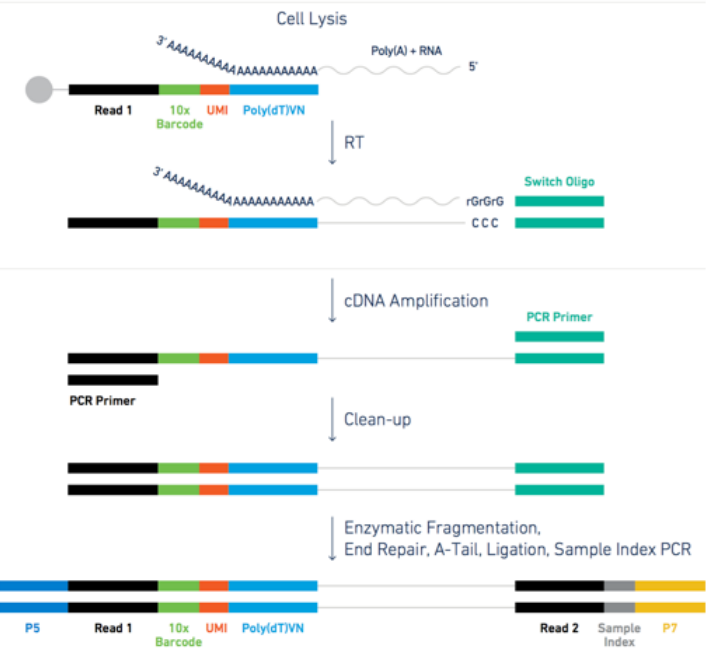
\includegraphics[width=6.25in,height=\textheight]{images/10X.png}

}

\caption{\label{fig-steps}steps for the microdroplet-based single cell
RNA sequencing after isolation.}

\end{figure}%

\subsection{The raw data in practice}\label{the-raw-data-in-practice}

Let's look at a specific read and its UMI and cell barcode. The data is
organized in paired-end reads (written on \texttt{fastq} files), where
the first \texttt{fastq} file contains reads in the following format

\begin{verbatim}
@SRR8363305.1 1 length=26
NTGAAGTGTTAAGACAAGCGTGAACT
+SRR8363305.1 1 length=26
#AAFFJJJJJJJJJJJJJJJJFJJJJ
\end{verbatim}

Here, the first 16 characters \texttt{NTGAAGTGTTAAGACA} represent the
cell barcode, while the last 10 characters \texttt{AGCGTGAACT} are the
transcript UMI tag. The last line represents the quality scores of the
26 characters of barcode+UMI.

The associated second \texttt{fastq} file contains reads of 98nt as the
following

\begin{verbatim}
@SRR8363305.1 1 length=98
NCTAAAGATCACACTAAGGCAACTCATGGAGGGGTCTTCAAAGA
    CCTTGCAAGAAGTACTAACTATGGAGTATCGGCTAAGTCAANCN
    TGTATGAGAT
+SRR8363305.1 1 length=98
#A<77AFJJFAAAJJJ7-7-<7FJ-7----<77--7FAAA--
    <JFFF-7--7<<-F77---FF---7-7A-777777A-<
    -7---#-#A-7-7--7--
\end{verbatim}

The 98nt-long string of characters in the second line is a partial
sequence of the cDNA transcript. Specifically, the 10X chromium protocol
used for sequencing the data is biased towards the 3' end, because the
sequencing is oriented from the 3' to the 5' end of the transcripts. The
last line contains the corresponding quality scores.

\subsection{Alignment and expression
matrix}\label{alignment-and-expression-matrix}

The data is aligned with \texttt{cellranger}, a completely automatized
\href{https://support.10xgenomics.com/single-cell-gene-expression/software/pipelines/latest/what-is-cell-ranger}{pipeline
implemented by 10X} for 10X-genomics data.

Apart from the data, the output contains an interactive document
reporting the quality of the data and a small preliminary UMAP plot and
clustering. In this report it is especially instructive to look at the
\textbf{knee plot}.

The knee plot is created by plotting the number of unique molecular
identifiers (UMIs) or reads against the number of cells sequenced,
sorted in descending order. The UMIs or reads are a measure of the
amount of RNA captured for each cell, and thus a measure of the quality
of the data. The plot typically shows a \textbf{steep slope at the
beginning, followed by a plateau, and then a gradual decrese into a
second slope and a final plateau}.

\begin{itemize}
\tightlist
\item
  The steep slope represents the initial cells that are of \textbf{high
  quality} and have the highest number of UMIs or reads.
\item
  The first plateau represents the cells that have \textbf{lower quality
  data}, and the gradual decrease represents the addition of droplets
  with even lower quality data.
\item
  Usually, beyond the first slope, you have droplets that are
  \textbf{either empty or of so poor quality}, that they are not worth
  keeping for analysis.
\item
  The height of the last plateau gives you an idea of the
  \textbf{presence of ambient RNA} inside droplets. If the last plateau
  is located high up, then the corresponding amount of UMIs consist of
  background ambient RNA which likely pollutes all cells in your data.
\end{itemize}

Below, the knee plot from the \texttt{control\ 1} sample used in this
analysis. You can see that around 10,000 cells with above
\textasciitilde1000 UMIs seems to be coinsidered of decent quality by
\texttt{cellranger} (the part of line coloured in blue). Note that the
last plateau is located at a very low amount of UMIs, meaning there is
not really any relevant contamination from ambient RNA.

\begin{figure}

\centering{

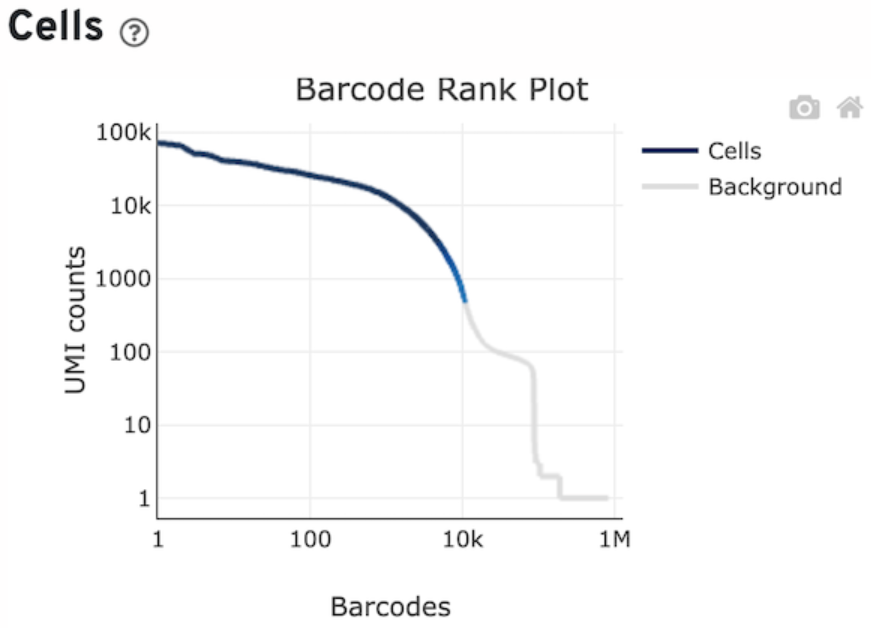
\includegraphics[width=6.25in,height=\textheight]{images/knee.png}

}

\caption{\label{fig-knee}Knee plot of the Control 1 sample of the
tutorial. Note the lower plateau of ambient RNA}

\end{figure}%

\begin{tcolorbox}[enhanced jigsaw, toprule=.15mm, coltitle=black, colframe=quarto-callout-note-color-frame, colback=white, colbacktitle=quarto-callout-note-color!10!white, opacityback=0, arc=.35mm, breakable, rightrule=.15mm, titlerule=0mm, leftrule=.75mm, bottomtitle=1mm, toptitle=1mm, title={Exercise}, bottomrule=.15mm, left=2mm, opacitybacktitle=0.6]

In this same folder you have the document \texttt{web\_summary.html}
that shows you the quality report of your own dataset. \textbf{Take some
time to look at it and explore what it contains} (Click on
\texttt{Trust\ HTML} on the top menu if the html remains blank after
opening it). Get an idea of how many UMIs there are in cells of decent
quality. We will work more on filtering out cells based on their quality
in this tutorial.

\end{tcolorbox}

\begin{tcolorbox}[enhanced jigsaw, toprule=.15mm, coltitle=black, colframe=quarto-callout-tip-color-frame, colback=white, colbacktitle=quarto-callout-tip-color!10!white, opacityback=0, arc=.35mm, breakable, rightrule=.15mm, titlerule=0mm, leftrule=.75mm, bottomtitle=1mm, toptitle=1mm, title=\textcolor{quarto-callout-tip-color}{\faLightbulb}\hspace{0.5em}{Something more about knee plots}, bottomrule=.15mm, left=2mm, opacitybacktitle=0.6]

The background RNA (sequenced together with the transcript coming from
the cell of interest) makes up the \emph{ambient plateau}: the same
background RNA is contained in empty droplets. If your dataset has
extremely few UMI counts in empty droplets, then there is not much
background RNA present - This is the best situation in which you can
find yourself. See Exhibit A in Figure~\ref{fig-bender}.

If you have a dataset where you can identify an \emph{empty droplet
plateau} by eye (Exhibit B in Figure~\ref{fig-bender}), and these empty
droplets have 50 or 100 or several hundred counts, then it can be
advisable to use a specific software to remove the background
transcripts (e.g.~\texttt{CellBender} (Fleming et al. (2023)),
\texttt{SoupX} (Young and Behjati (2020))).

If you have a dataset with so much background RNA that you cannot
identify the \emph{empty droplet plateau} yourself by eye (Exhibit C in
Figure~\ref{fig-bender}), then any software to remove background
transcripts will also likely have a difficult time. Such the algorithms
might be worth a try, but you should \textbf{strongly consider
re-running the experiment, as the knee plot points to a real QC failure}

\begin{figure}[H]

\centering{

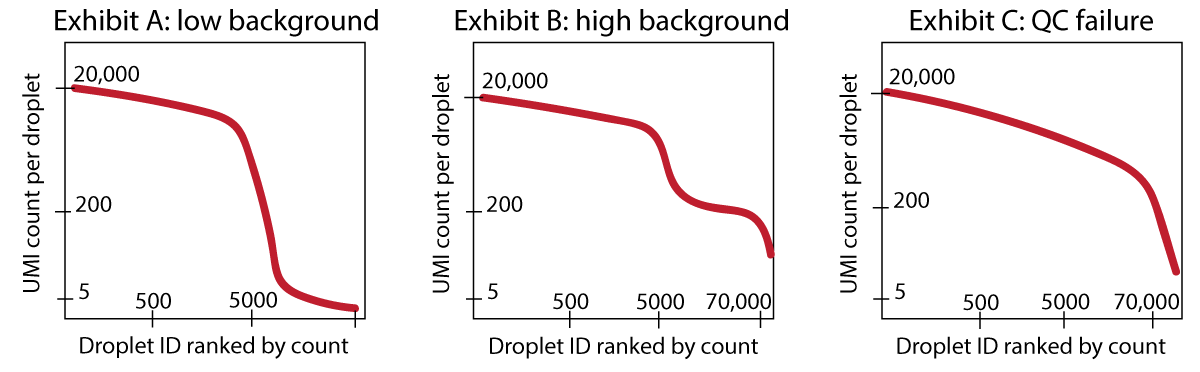
\includegraphics[width=6.25in,height=\textheight]{images/UMI_curve_tropes.png}

}

\caption{\label{fig-bender}Various cases of knee plot you can encounter
from sequenced data. Figure from
\href{https://cellbender.readthedocs.io/}{the webpage of Cellbender.}}

\end{figure}%

\end{tcolorbox}

\section{Preprocessing}\label{sec-preprocessing}

\begin{tcolorbox}[enhanced jigsaw, toprule=.15mm, coltitle=black, colframe=quarto-callout-note-color-frame, colback=white, colbacktitle=quarto-callout-note-color!10!white, opacityback=0, arc=.35mm, breakable, rightrule=.15mm, titlerule=0mm, leftrule=.75mm, bottomtitle=1mm, toptitle=1mm, title=\textcolor{quarto-callout-note-color}{\faInfo}\hspace{0.5em}{Learning outcome}, bottomrule=.15mm, left=2mm, opacitybacktitle=0.6]

We will answer to the following questions:

\begin{itemize}
\tightlist
\item
  How can I \textbf{import single-cell data} into R?
\item
  How are different types of data/information (e.g.~cell information,
  gene information, etc.) \textbf{stored and manipulated}?
\item
  How can I obtain basic \textbf{summary metrics} for cells and genes
  and \textbf{filter the data} accordingly?
\item
  How can I \textbf{visually explore} these metrics?
\end{itemize}

\end{tcolorbox}

We start by loading all the packages necessary for the analysis and
setup a few things

\begin{Shaded}
\begin{Highlighting}[]
\FunctionTok{suppressPackageStartupMessages}\NormalTok{(\{}
\FunctionTok{library}\NormalTok{(SeuratDisk); }
\FunctionTok{library}\NormalTok{(Seurat);}
\FunctionTok{library}\NormalTok{(DoubletFinder);}
\FunctionTok{library}\NormalTok{(parallel);}
\FunctionTok{library}\NormalTok{(multtest);}
\FunctionTok{library}\NormalTok{(metap);}
\FunctionTok{library}\NormalTok{(purrr);}
\FunctionTok{library}\NormalTok{(dplyr);}
\FunctionTok{library}\NormalTok{(stringr);}
\FunctionTok{library}\NormalTok{(tibble);}
\FunctionTok{library}\NormalTok{(ggplot2);}
\FunctionTok{library}\NormalTok{(MAST);}
\FunctionTok{library}\NormalTok{(WGCNA);}
\FunctionTok{library}\NormalTok{(hdWGCNA);}
\FunctionTok{library}\NormalTok{(patchwork);}
\FunctionTok{library}\NormalTok{(doFuture);\})}
\end{Highlighting}
\end{Shaded}

\begin{Shaded}
\begin{Highlighting}[]
\FunctionTok{source}\NormalTok{(}\StringTok{"../Scripts/script.R"}\NormalTok{)}
\end{Highlighting}
\end{Shaded}

\begin{Shaded}
\begin{Highlighting}[]
\FunctionTok{options}\NormalTok{(}\AttributeTok{future.seed=}\ConstantTok{TRUE}\NormalTok{)}
\end{Highlighting}
\end{Shaded}

\begin{Shaded}
\begin{Highlighting}[]
\FunctionTok{plan}\NormalTok{(}\StringTok{"multicore"}\NormalTok{, }\AttributeTok{workers =} \DecValTok{8}\NormalTok{)}
\FunctionTok{options}\NormalTok{(}\AttributeTok{future.globals.maxSize =} \DecValTok{8} \SpecialCharTok{*} \DecValTok{1024}\SpecialCharTok{\^{}}\DecValTok{3}\NormalTok{)}
\end{Highlighting}
\end{Shaded}

\subsection{Import data}\label{import-data}

We import the data reading the matrix files aligned by 10X. Those are
usually contained in a folder with a name of the type
\texttt{aligned\_dataset/outs/filtered\_bc\_matrix}, that 10X Cellranger
creates automatically after the alignment. You will use such a folder
when your own data is aligned. In this tutorial, the aligned data is in
the folder used below. The command for reading the data is simply
\texttt{Read10X}.

\begin{tcolorbox}[enhanced jigsaw, toprule=.15mm, coltitle=black, colframe=quarto-callout-important-color-frame, colback=white, colbacktitle=quarto-callout-important-color!10!white, opacityback=0, arc=.35mm, breakable, rightrule=.15mm, titlerule=0mm, leftrule=.75mm, bottomtitle=1mm, toptitle=1mm, title=\textcolor{quarto-callout-important-color}{\faExclamation}\hspace{0.5em}{Important}, bottomrule=.15mm, left=2mm, opacitybacktitle=0.6]

When using your own data, you need to use the correct folder name below
according to the \texttt{10X} folder structure
\texttt{aligned\_dataset/outs/filtered\_bc\_matrix}.

\end{tcolorbox}

\begin{Shaded}
\begin{Highlighting}[]
\NormalTok{Control1 }\OtherTok{\textless{}{-}} \FunctionTok{Read10X}\NormalTok{(}\StringTok{"../Data/control\_1/"}\NormalTok{)}
\end{Highlighting}
\end{Shaded}

Note that we are loading only one dataset (\texttt{control\_1}, one of
the two control replicates). Another control dataset, and two infected
datasets, have already been preprocessed and will be used later - so
\textbf{we will now focus on the preprocessing of a single dataset}. In
general, when you have multiple datasets, you must preprocess them one
at a time before integrating them together.

What we obtain in the command above is an expression matrix. Look at the
first 10 rows and columns of the matrix (whose rows represent genes and
columns droplets/cells) - the dots are zeros (they are not stored in the
data, which has a compressed format called \texttt{dgCMatrix}), and
\textbf{are the majority of the expression values obtained in scRNA
data!}

\begin{Shaded}
\begin{Highlighting}[]
\NormalTok{Control1[}\DecValTok{1}\SpecialCharTok{:}\DecValTok{10}\NormalTok{,}\DecValTok{1}\SpecialCharTok{:}\DecValTok{10}\NormalTok{]}
\end{Highlighting}
\end{Shaded}

\begin{verbatim}
  [[ suppressing 10 column names ‘AAACCCAAGGGCAGTT-1’, ‘AAACCCAAGTCAGCGA-1’, ‘AAACCCACACTAACCA-1’ ... ]]
\end{verbatim}

\begin{verbatim}
10 x 10 sparse Matrix of class "dgCMatrix"
                                         
LotjaGi0g1v0000100    . . . . . . . . . .
LotjaGi0g1v0000200    . . . . . . . . . .
LotjaGi0g1v0000300    . . . . . . . . . .
LotjaGi0g1v0000400    . . . . . . 1 1 . .
LotjaGi0g1v0000500    . . . . . . . . . .
LotjaGi0g1v0000600    . . . . . . . . . .
LotjaGi0g1v0000700    . . . . . . . . . .
LotjaGi0g1v0000800    . . . . 1 . . . . .
LotjaGi0g1v0000900_LC . . . . . . . . . .
LotjaGi0g1v0001000_LC . . . . . . . . . .
\end{verbatim}

What is the percentage of zeros in this matrix? You can see it for
yourself below - it is a lot, but quite surprisingly we can get a lot of
information from the data!

\begin{Shaded}
\begin{Highlighting}[]
\FunctionTok{cat}\NormalTok{(}\StringTok{"Number of zeros: "}\NormalTok{)}
\NormalTok{zeros }\OtherTok{\textless{}{-}}  \FunctionTok{sum}\NormalTok{(Control1}\SpecialCharTok{==}\DecValTok{0}\NormalTok{)}
\FunctionTok{cat}\NormalTok{( zeros )}
\end{Highlighting}
\end{Shaded}

\begin{verbatim}
Number of zeros: 307060673
\end{verbatim}

\begin{Shaded}
\begin{Highlighting}[]
\FunctionTok{cat}\NormalTok{(}\StringTok{"Number of expression entries: "}\NormalTok{)}
\NormalTok{total }\OtherTok{\textless{}{-}} \FunctionTok{dim}\NormalTok{(Control1)[}\DecValTok{1}\NormalTok{] }\SpecialCharTok{*} \FunctionTok{dim}\NormalTok{(Control1)[}\DecValTok{2}\NormalTok{]}
\FunctionTok{cat}\NormalTok{( total )}
\end{Highlighting}
\end{Shaded}

\begin{verbatim}
Number of expression entries: 329798055
\end{verbatim}

\begin{Shaded}
\begin{Highlighting}[]
\FunctionTok{cat}\NormalTok{(}\StringTok{"Percentage of zeros: "}\NormalTok{)}
\FunctionTok{cat}\NormalTok{( zeros }\SpecialCharTok{/}\NormalTok{ total }\SpecialCharTok{*} \DecValTok{100}\NormalTok{ )}
\end{Highlighting}
\end{Shaded}

\begin{verbatim}
Percentage of zeros: 93.10567
\end{verbatim}

\subsection{Create a single cell object in
Seurat}\label{create-a-single-cell-object-in-seurat}

We use our count matrix to create a Seurat object. A Seurat object
allows you to \textbf{store the count matrix} and future modifications
of it (for example its normalized version), together with
\textbf{information regarding cells and genes} (such as clusters of cell
types) and their \textbf{projections} (such as PCA and tSNE). We will go
through these elements, but first we create the object with
\texttt{CreateSeuratObject}:

\begin{Shaded}
\begin{Highlighting}[]
\NormalTok{Control1\_seurat }\OtherTok{\textless{}{-}} \FunctionTok{CreateSeuratObject}\NormalTok{(}\AttributeTok{counts =}\NormalTok{ Control1, }
                                               \AttributeTok{project =} \StringTok{"Control1\_seurat"}\NormalTok{, }
                                               \AttributeTok{min.cells =} \DecValTok{3}\NormalTok{, }
                                               \AttributeTok{min.features =} \DecValTok{200}\NormalTok{)}
\end{Highlighting}
\end{Shaded}

\begin{verbatim}
Warning message:
“Feature names cannot have underscores ('_'), replacing with dashes ('-')”
Warning message:
“Feature names cannot have underscores ('_'), replacing with dashes ('-')”
\end{verbatim}

The arguments of the command are * \texttt{counts}: the count matrix *
\texttt{project}: a project name * \texttt{min.cells}: a minimum
requirement for genes, in our case saying they must be expressed in at
least 3 cells. If not, they are filtered out already now when creating
the object. * \texttt{min.features}: a minimum requirement for cells.
Cells having less than 200 expressed genes are removed from the
beginning from the data.

Values for the minimum requirements chosen above are standard checks
when running the analysis. Droplets not satisfying those requirements
are of extremely bad quality and not worth carrying on during the
analysis (remember the knee plot).

How many genes and cells have been filtered out?

\begin{Shaded}
\begin{Highlighting}[]
\FunctionTok{cat}\NormalTok{(}\StringTok{"Starting Genes and Cells:}\SpecialCharTok{\textbackslash{}n}\StringTok{"}\NormalTok{)}
\FunctionTok{cat}\NormalTok{( }\FunctionTok{dim}\NormalTok{(Control1) )}

\FunctionTok{cat}\NormalTok{(}\StringTok{"}\SpecialCharTok{\textbackslash{}n}\StringTok{Filtered Genes and Cells:}\SpecialCharTok{\textbackslash{}n}\StringTok{"}\NormalTok{)}
\FunctionTok{cat}\NormalTok{( }\FunctionTok{dim}\NormalTok{(Control1) }\SpecialCharTok{{-}} \FunctionTok{dim}\NormalTok{(Control1\_seurat) )}

\FunctionTok{cat}\NormalTok{(}\StringTok{"}\SpecialCharTok{\textbackslash{}n}\StringTok{Remaining Genes and Cells:}\SpecialCharTok{\textbackslash{}n}\StringTok{"}\NormalTok{)}
\FunctionTok{cat}\NormalTok{( }\FunctionTok{dim}\NormalTok{(Control1\_seurat) )}
\end{Highlighting}
\end{Shaded}

\begin{verbatim}
Starting Genes and Cells:
30585 10783
Filtered Genes and Cells:
6747 11
Remaining Genes and Cells:
23838 10772
\end{verbatim}

We want to use this data later in the analysis with other
\texttt{Control} and \texttt{Infected} datasets. Therefore we add a
\texttt{Condition} to the metadata table, and for this dataset we
establish that each cell is \texttt{Control}.

\begin{tcolorbox}[enhanced jigsaw, toprule=.15mm, coltitle=black, colframe=quarto-callout-important-color-frame, colback=white, colbacktitle=quarto-callout-important-color!10!white, opacityback=0, arc=.35mm, breakable, rightrule=.15mm, titlerule=0mm, leftrule=.75mm, bottomtitle=1mm, toptitle=1mm, title=\textcolor{quarto-callout-important-color}{\faExclamation}\hspace{0.5em}{Important}, bottomrule=.15mm, left=2mm, opacitybacktitle=0.6]

When using your own data, do not forget to \textbf{write the correct
condition label}.

\end{tcolorbox}

\begin{Shaded}
\begin{Highlighting}[]
\NormalTok{Control1\_seurat }\OtherTok{\textless{}{-}} \FunctionTok{AddMetaData}\NormalTok{(}\AttributeTok{object =}\NormalTok{ Control1\_seurat, }
                                        \AttributeTok{metadata =} \StringTok{"Control"}\NormalTok{, }
                                        \AttributeTok{col.name =} \StringTok{"Condition"}\NormalTok{)}
\end{Highlighting}
\end{Shaded}

\subsubsection{Content of a Seurat
Object}\label{content-of-a-seurat-object}

What is contained in the Seurat object? We can use the command
\texttt{str} to list the various \emph{slots} of the object.

\begin{Shaded}
\begin{Highlighting}[]
\FunctionTok{str}\NormalTok{(Control1\_seurat, }\AttributeTok{max.level =} \DecValTok{2}\NormalTok{)}
\end{Highlighting}
\end{Shaded}

\begin{verbatim}
Formal class 'Seurat' [package "SeuratObject"] with 13 slots
  ..@ assays      :List of 1
  ..@ meta.data   :'data.frame':    10772 obs. of  4 variables:
  ..@ active.assay: chr "RNA"
  ..@ active.ident: Factor w/ 1 level "Control1_seurat": 1 1 1 1 1 1 1 1 1 1 ...
  .. ..- attr(*, "names")= chr [1:10772] "AAACCCAAGGGCAGTT-1" "AAACCCAAGTCAGCGA-1" "AAACCCACACTAACCA-1" "AAACCCACATGATCTG-1" ...
  ..@ graphs      : list()
  ..@ neighbors   : list()
  ..@ reductions  : list()
  ..@ images      : list()
  ..@ project.name: chr "Control1_seurat"
  ..@ misc        : list()
  ..@ version     :Classes 'package_version', 'numeric_version'  hidden list of 1
  ..@ commands    : list()
  ..@ tools       : list()
\end{verbatim}

The first slot is called \texttt{assays}, and it contains all the count
matrices we have collected during our analysis when, for example,
normalizing data or doing other transformations of it. Right now we only
have the \texttt{RNA} assay with the raw counts:

\begin{Shaded}
\begin{Highlighting}[]
\NormalTok{Control1\_seurat}\SpecialCharTok{@}\NormalTok{assays}
\end{Highlighting}
\end{Shaded}

\begin{verbatim}
$RNA
Assay data with 23838 features for 10772 cells
First 10 features:
 LotjaGi0g1v0000100, LotjaGi0g1v0000200, LotjaGi0g1v0000300,
LotjaGi0g1v0000400, LotjaGi0g1v0000500, LotjaGi0g1v0000700,
LotjaGi0g1v0000800, LotjaGi0g1v0001100, LotjaGi0g1v0001200,
LotjaGi0g1v0001400 
\end{verbatim}

You can always select which matrix is currently in use for the analysis
by assigning it to \texttt{DefaultAssay()}. The default assay is often
changed automatically by Seurat, for example the normalized assay is
used as default after normalization is performed.

\begin{Shaded}
\begin{Highlighting}[]
\FunctionTok{DefaultAssay}\NormalTok{(}\AttributeTok{object =}\NormalTok{ Control1\_seurat) }\OtherTok{\textless{}{-}} \StringTok{"RNA"}
\end{Highlighting}
\end{Shaded}

\begin{Shaded}
\begin{Highlighting}[]
\FunctionTok{cat}\NormalTok{(}\StringTok{"Your default assay is "}\NormalTok{)}
\FunctionTok{cat}\NormalTok{(}\FunctionTok{DefaultAssay}\NormalTok{(}\AttributeTok{object =}\NormalTok{ Control1\_seurat))}
\end{Highlighting}
\end{Shaded}

\begin{verbatim}
Your default assay is RNA
\end{verbatim}

The second slot is the one that contains the metadata for each cell. It
is easily visualized as a table (the command \texttt{head} shows only
the first 6 rows of the table):

\begin{Shaded}
\begin{Highlighting}[]
\FunctionTok{head}\NormalTok{( Control1\_seurat}\SpecialCharTok{@}\NormalTok{meta.data )}
\end{Highlighting}
\end{Shaded}

A data.frame: 6 × 4

\begin{longtable}[]{@{}
  >{\raggedright\arraybackslash}p{(\columnwidth - 8\tabcolsep) * \real{0.2000}}
  >{\raggedright\arraybackslash}p{(\columnwidth - 8\tabcolsep) * \real{0.2000}}
  >{\raggedright\arraybackslash}p{(\columnwidth - 8\tabcolsep) * \real{0.2000}}
  >{\raggedright\arraybackslash}p{(\columnwidth - 8\tabcolsep) * \real{0.2000}}
  >{\raggedright\arraybackslash}p{(\columnwidth - 8\tabcolsep) * \real{0.2000}}@{}}
\toprule\noalign{}
\begin{minipage}[b]{\linewidth}\raggedright
\end{minipage} & \begin{minipage}[b]{\linewidth}\raggedright
orig.ident \textless fct\textgreater{}
\end{minipage} & \begin{minipage}[b]{\linewidth}\raggedright
nCount\_RNA \textless dbl\textgreater{}
\end{minipage} & \begin{minipage}[b]{\linewidth}\raggedright
nFeature\_RNA \textless int\textgreater{}
\end{minipage} & \begin{minipage}[b]{\linewidth}\raggedright
Condition \textless chr\textgreater{}
\end{minipage} \\
\midrule\noalign{}
\endhead
\bottomrule\noalign{}
\endlastfoot
AAACCCAAGGGCAGTT-1 & Control1\_seurat & 3567 & 1919 & Control \\
AAACCCAAGTCAGCGA-1 & Control1\_seurat & 7015 & 2751 & Control \\
AAACCCACACTAACCA-1 & Control1\_seurat & 1484 & 828 & Control \\
AAACCCACATGATCTG-1 & Control1\_seurat & 20942 & 4711 & Control \\
AAACCCAGTAGCTTGT-1 & Control1\_seurat & 29105 & 5157 & Control \\
AAACCCAGTCTCTCAC-1 & Control1\_seurat & 6115 & 2124 & Control \\
\end{longtable}

The table contains a name for the dataset (\texttt{orig.ident}, useful
to distinguish multiple datasets merged together), how many RNA
transcripts are contained in each cell (\texttt{nCount\_RNA}), the
number of expressed genes in each cell (\texttt{nFeature\_RNA}), and the
\texttt{Condition} (added by us previously). More metadata can be added
along the analysis, and some is added automatically by Seurat when
running specific commands.

The \texttt{assays} and \texttt{meta.data} slots are the most relevant
and useful to know - the other ones are mostly for internal use by
Seurat and we do not go into detail with those.

\subsection{Finding filtering
criteria}\label{finding-filtering-criteria}

We want to look in depth at which droplets do not contain good quality
data, so that we can filter them out. The standard approach - which
works quite well - is to study the \textbf{distribution of various
quality measures and remove doublets} (droplets containing more than one
cell) which can confound the analysis results. We will look at some
plots and decide some threshold, then we will apply them at the end
after looking at all the histograms.

\subsubsection{Quality measure
distributions}\label{quality-measure-distributions}

A first step is to calculate the percentage of mitochondrial and
chloroplastic genes. A high percentage indicates the presence of spilled
material from broken cells. We use the command
\texttt{PercentageFeatureSet} and provide the pattern of the gene ID
which corresponds to mitochondrial and ribosomal genes. The percentages
are saved into the metadata simply by using the double squared brackets
\texttt{{[}{[}}.

\begin{Shaded}
\begin{Highlighting}[]
\NormalTok{Control1\_seurat[[}\StringTok{"percent.mt"}\NormalTok{]] }\OtherTok{\textless{}{-}} \FunctionTok{PercentageFeatureSet}\NormalTok{(Control1\_seurat, }
                                                                 \AttributeTok{pattern =} \StringTok{"LotjaGiM1v"}\NormalTok{)}
\NormalTok{Control1\_seurat[[}\StringTok{"percent.chloroplast"}\NormalTok{]] }\OtherTok{\textless{}{-}} \FunctionTok{PercentageFeatureSet}\NormalTok{(Control1\_seurat, }
                                                                          \AttributeTok{pattern =} \StringTok{"LotjaGiC1v"}\NormalTok{)}
\end{Highlighting}
\end{Shaded}

You can see the new metadata is now added for each cell

\begin{Shaded}
\begin{Highlighting}[]
\FunctionTok{head}\NormalTok{( Control1\_seurat}\SpecialCharTok{@}\NormalTok{meta.data )}
\end{Highlighting}
\end{Shaded}

A data.frame: 6 × 6

\begin{longtable}[]{@{}
  >{\raggedright\arraybackslash}p{(\columnwidth - 12\tabcolsep) * \real{0.1429}}
  >{\raggedright\arraybackslash}p{(\columnwidth - 12\tabcolsep) * \real{0.1429}}
  >{\raggedright\arraybackslash}p{(\columnwidth - 12\tabcolsep) * \real{0.1429}}
  >{\raggedright\arraybackslash}p{(\columnwidth - 12\tabcolsep) * \real{0.1429}}
  >{\raggedright\arraybackslash}p{(\columnwidth - 12\tabcolsep) * \real{0.1429}}
  >{\raggedright\arraybackslash}p{(\columnwidth - 12\tabcolsep) * \real{0.1429}}
  >{\raggedright\arraybackslash}p{(\columnwidth - 12\tabcolsep) * \real{0.1429}}@{}}
\toprule\noalign{}
\begin{minipage}[b]{\linewidth}\raggedright
\end{minipage} & \begin{minipage}[b]{\linewidth}\raggedright
orig.ident \textless fct\textgreater{}
\end{minipage} & \begin{minipage}[b]{\linewidth}\raggedright
nCount\_RNA \textless dbl\textgreater{}
\end{minipage} & \begin{minipage}[b]{\linewidth}\raggedright
nFeature\_RNA \textless int\textgreater{}
\end{minipage} & \begin{minipage}[b]{\linewidth}\raggedright
Condition \textless chr\textgreater{}
\end{minipage} & \begin{minipage}[b]{\linewidth}\raggedright
percent.mt \textless dbl\textgreater{}
\end{minipage} & \begin{minipage}[b]{\linewidth}\raggedright
percent.chloroplast \textless dbl\textgreater{}
\end{minipage} \\
\midrule\noalign{}
\endhead
\bottomrule\noalign{}
\endlastfoot
AAACCCAAGGGCAGTT-1 & Control1\_seurat & 3567 & 1919 & Control &
4.6818054 & 0.02803476 \\
AAACCCAAGTCAGCGA-1 & Control1\_seurat & 7015 & 2751 & Control &
0.7127584 & 0.04276550 \\
AAACCCACACTAACCA-1 & Control1\_seurat & 1484 & 828 & Control & 6.6037736
& 0.06738544 \\
AAACCCACATGATCTG-1 & Control1\_seurat & 20942 & 4711 & Control &
0.4775093 & 0.12415242 \\
AAACCCAGTAGCTTGT-1 & Control1\_seurat & 29105 & 5157 & Control &
0.2954819 & 0.05497337 \\
AAACCCAGTCTCTCAC-1 & Control1\_seurat & 6115 & 2124 & Control &
1.6026165 & 0.01635323 \\
\end{longtable}

\paragraph{Number of transcripts per
cell}\label{number-of-transcripts-per-cell}

We plot a histogram of the number of transcripts per cell in
Figure~\ref{fig-rnacount} below. On the right, we zoom into the
histogram. We want to \textbf{filter out the cells with the lowest
number of transcripts} - often there is a peak we can identify with a
group of low-quality cells. Here we can choose to remove cells with less
than \textasciitilde700 transcripts (some people prefere to do a lighter
filtering, and would for example set a threshold to a lower value). We
remove also \textbf{cells with too many transcripts} that might contain
some weird transcripts - which is also helpful for normalization because
it removes some outlying values. For those we can set a limit to 30000,
where there is a very thin tail in the histogram.

\begin{Shaded}
\begin{Highlighting}[]
\FunctionTok{options}\NormalTok{(}\AttributeTok{repr.plot.width=}\DecValTok{14}\NormalTok{, }\AttributeTok{repr.plot.height=}\DecValTok{5}\NormalTok{)}

\NormalTok{plot1 }\OtherTok{\textless{}{-}} \FunctionTok{ggplot}\NormalTok{(Control1\_seurat}\SpecialCharTok{@}\NormalTok{meta.data, }\FunctionTok{aes}\NormalTok{(}\AttributeTok{x=}\NormalTok{nCount\_RNA)) }\SpecialCharTok{+} 
     \FunctionTok{geom\_histogram}\NormalTok{(}\AttributeTok{fill=}\StringTok{"\#69b3a2"}\NormalTok{, }\AttributeTok{color=}\StringTok{"\#e9ecef"}\NormalTok{, }\AttributeTok{alpha=}\FloatTok{0.9}\NormalTok{)}

\NormalTok{plot2 }\OtherTok{\textless{}{-}} \FunctionTok{ggplot}\NormalTok{(Control1\_seurat}\SpecialCharTok{@}\NormalTok{meta.data, }\FunctionTok{aes}\NormalTok{(}\AttributeTok{x=}\NormalTok{nCount\_RNA)) }\SpecialCharTok{+} 
     \FunctionTok{geom\_histogram}\NormalTok{(}\AttributeTok{fill=}\StringTok{"\#69b3a2"}\NormalTok{, }\AttributeTok{color=}\StringTok{"\#e9ecef"}\NormalTok{, }\AttributeTok{alpha=}\FloatTok{0.9}\NormalTok{) }\SpecialCharTok{+}
     \FunctionTok{xlim}\NormalTok{(}\DecValTok{0}\NormalTok{,}\DecValTok{2000}\NormalTok{)}

\NormalTok{plot1 }\SpecialCharTok{+}\NormalTok{ plot2}
\end{Highlighting}
\end{Shaded}

\begin{verbatim}
`stat_bin()` using `bins = 30`. Pick better value with `binwidth`.
`stat_bin()` using `bins = 30`. Pick better value with `binwidth`.
Warning message:
“Removed 7668 rows containing non-finite values (`stat_bin()`).”
Warning message:
“Removed 2 rows containing missing values (`geom_bar()`).”
\end{verbatim}

\begin{figure}[H]

\centering{

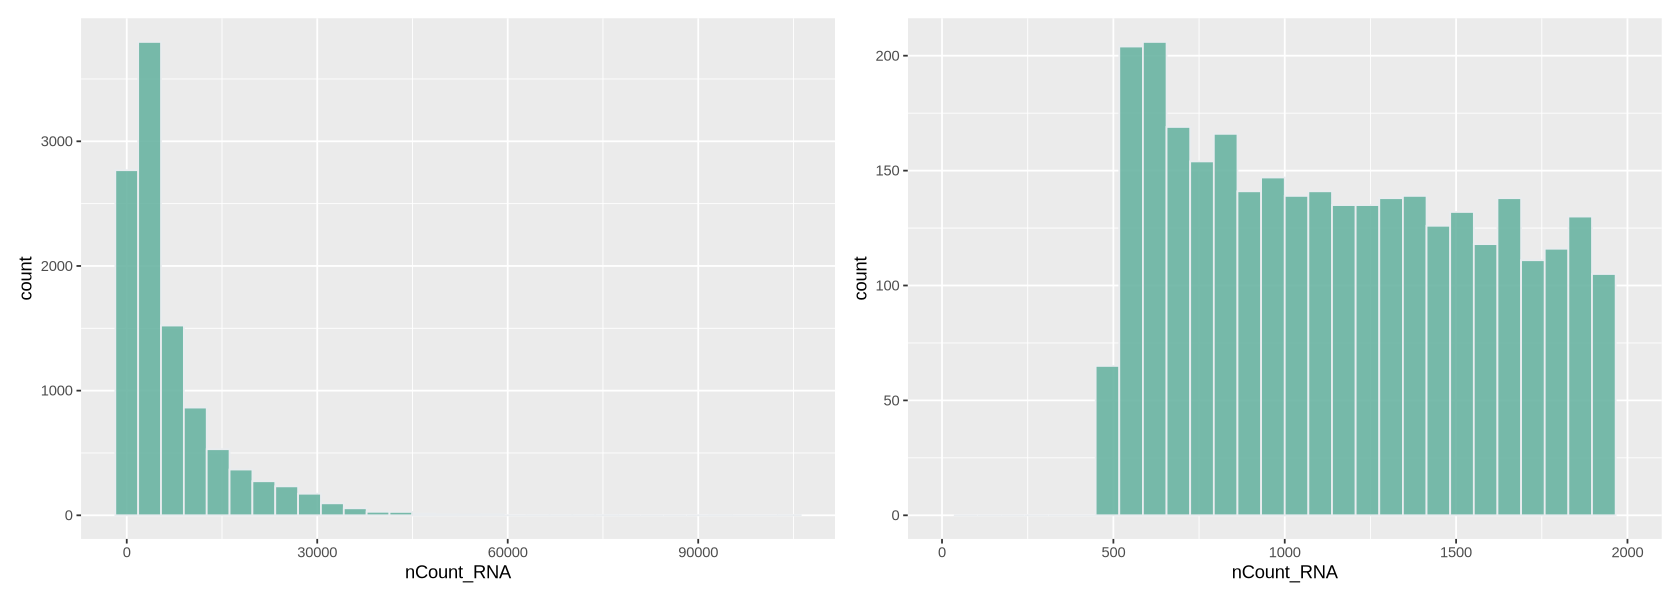
\includegraphics{tutorial-2024_files/figure-pdf/fig-rnacount-output-2.png}

}

\caption{\label{fig-rnacount}Histogram of transcripts per cell (left)
and a zoom onto the histogram (right)}

\end{figure}%

\paragraph{Number of detected genes per
cell}\label{number-of-detected-genes-per-cell}

Here we work similarly to filter out cells based on how many genes are
detected (Figure~\ref{fig-genecounts}). The right-side plot is a zoom
into the histogram. It seems easy to set the thresholds at
\textasciitilde400 and \textasciitilde7000 detected genes.

\begin{Shaded}
\begin{Highlighting}[]
\FunctionTok{options}\NormalTok{(}\AttributeTok{repr.plot.width=}\DecValTok{14}\NormalTok{, }\AttributeTok{repr.plot.height=}\DecValTok{5}\NormalTok{)}

\NormalTok{plot1 }\OtherTok{\textless{}{-}} \FunctionTok{ggplot}\NormalTok{(Control1\_seurat}\SpecialCharTok{@}\NormalTok{meta.data, }\FunctionTok{aes}\NormalTok{(}\AttributeTok{x=}\NormalTok{nFeature\_RNA)) }\SpecialCharTok{+} 
     \FunctionTok{geom\_histogram}\NormalTok{(}\AttributeTok{fill=}\StringTok{"\#69b3a2"}\NormalTok{, }\AttributeTok{color=}\StringTok{"\#e9ecef"}\NormalTok{, }\AttributeTok{alpha=}\FloatTok{0.9}\NormalTok{)}

\NormalTok{plot2 }\OtherTok{\textless{}{-}} \FunctionTok{ggplot}\NormalTok{(Control1\_seurat}\SpecialCharTok{@}\NormalTok{meta.data, }\FunctionTok{aes}\NormalTok{(}\AttributeTok{x=}\NormalTok{nFeature\_RNA)) }\SpecialCharTok{+} 
     \FunctionTok{geom\_histogram}\NormalTok{(}\AttributeTok{fill=}\StringTok{"\#69b3a2"}\NormalTok{, }\AttributeTok{color=}\StringTok{"\#e9ecef"}\NormalTok{, }\AttributeTok{alpha=}\FloatTok{0.9}\NormalTok{) }\SpecialCharTok{+}
     \FunctionTok{xlim}\NormalTok{(}\DecValTok{0}\NormalTok{,}\DecValTok{1000}\NormalTok{)}


\NormalTok{plot1 }\SpecialCharTok{+}\NormalTok{ plot2}
\end{Highlighting}
\end{Shaded}

\begin{verbatim}
`stat_bin()` using `bins = 30`. Pick better value with `binwidth`.
`stat_bin()` using `bins = 30`. Pick better value with `binwidth`.
Warning message:
“Removed 7793 rows containing non-finite values (`stat_bin()`).”
Warning message:
“Removed 2 rows containing missing values (`geom_bar()`).”
\end{verbatim}

\begin{figure}[H]

\centering{

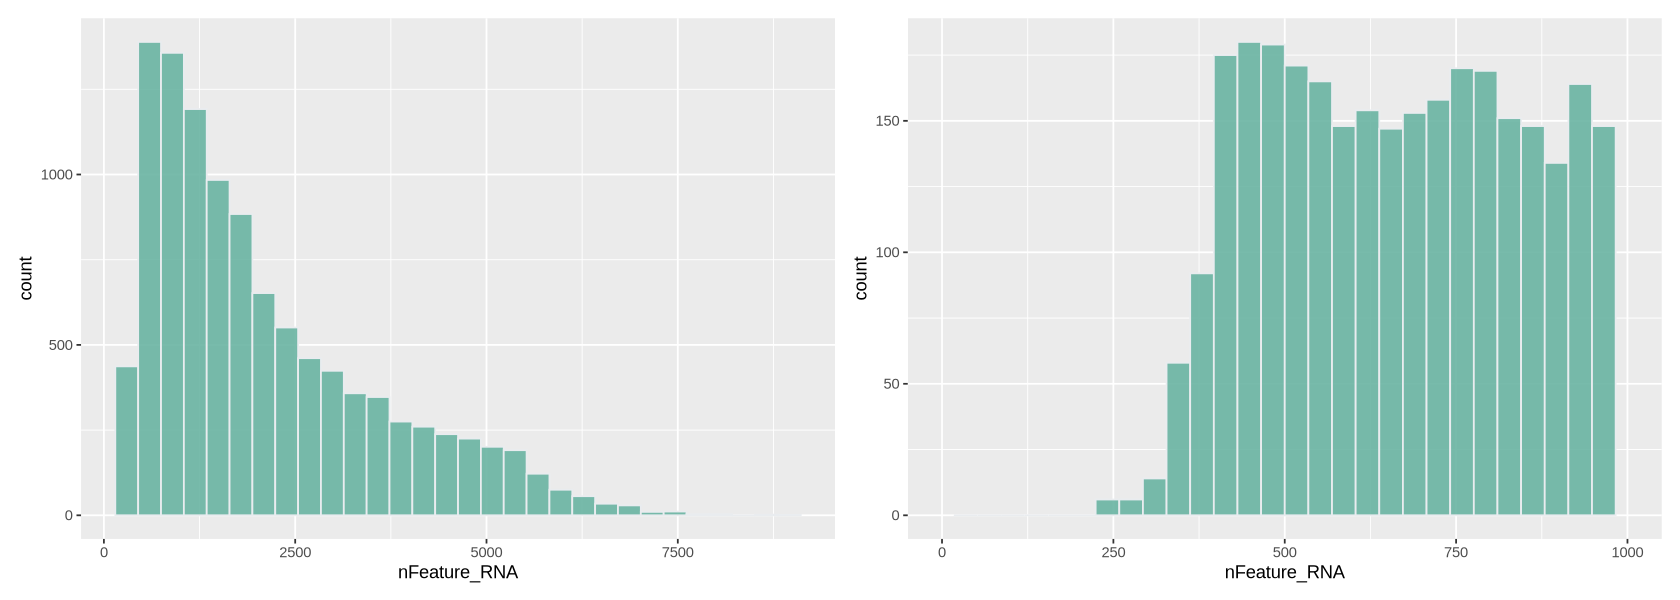
\includegraphics{tutorial-2024_files/figure-pdf/fig-genecounts-output-2.png}

}

\caption{\label{fig-genecounts}Histogram of detected counts per cell
(left) and a zoom onto the histogram (right)}

\end{figure}%

\paragraph{Mitochondrial and Chloroplast
percentages}\label{mitochondrial-and-chloroplast-percentages}

The percentages of mitochondrial and chloroplastic transcripts tells us
the data is of good quality, since most cells have low values of those
(Figure~\ref{fig-mt}). Thresholds are usually set between 5\% and 20\%
in single cell data analysis. In the paper, thresholds were for example
set at 20\%.

\begin{Shaded}
\begin{Highlighting}[]
\FunctionTok{options}\NormalTok{(}\AttributeTok{repr.plot.width=}\DecValTok{14}\NormalTok{, }\AttributeTok{repr.plot.height=}\DecValTok{5}\NormalTok{)}

\NormalTok{plot1 }\OtherTok{\textless{}{-}} \FunctionTok{ggplot}\NormalTok{(Control1\_seurat}\SpecialCharTok{@}\NormalTok{meta.data, }\FunctionTok{aes}\NormalTok{(}\AttributeTok{x=}\NormalTok{percent.mt)) }\SpecialCharTok{+} 
     \FunctionTok{geom\_histogram}\NormalTok{(}\AttributeTok{fill=}\StringTok{"\#69b3a2"}\NormalTok{, }\AttributeTok{color=}\StringTok{"\#e9ecef"}\NormalTok{, }\AttributeTok{alpha=}\FloatTok{0.9}\NormalTok{)}

\NormalTok{plot2 }\OtherTok{\textless{}{-}} \FunctionTok{ggplot}\NormalTok{(Control1\_seurat}\SpecialCharTok{@}\NormalTok{meta.data, }\FunctionTok{aes}\NormalTok{(}\AttributeTok{x=}\NormalTok{percent.chloroplast)) }\SpecialCharTok{+} 
     \FunctionTok{geom\_histogram}\NormalTok{(}\AttributeTok{fill=}\StringTok{"\#69b3a2"}\NormalTok{, }\AttributeTok{color=}\StringTok{"\#e9ecef"}\NormalTok{, }\AttributeTok{alpha=}\FloatTok{0.9}\NormalTok{)}

\NormalTok{plot1 }\SpecialCharTok{+}\NormalTok{ plot2}
\end{Highlighting}
\end{Shaded}

\begin{verbatim}
`stat_bin()` using `bins = 30`. Pick better value with `binwidth`.
`stat_bin()` using `bins = 30`. Pick better value with `binwidth`.
\end{verbatim}

\begin{figure}[H]

\centering{

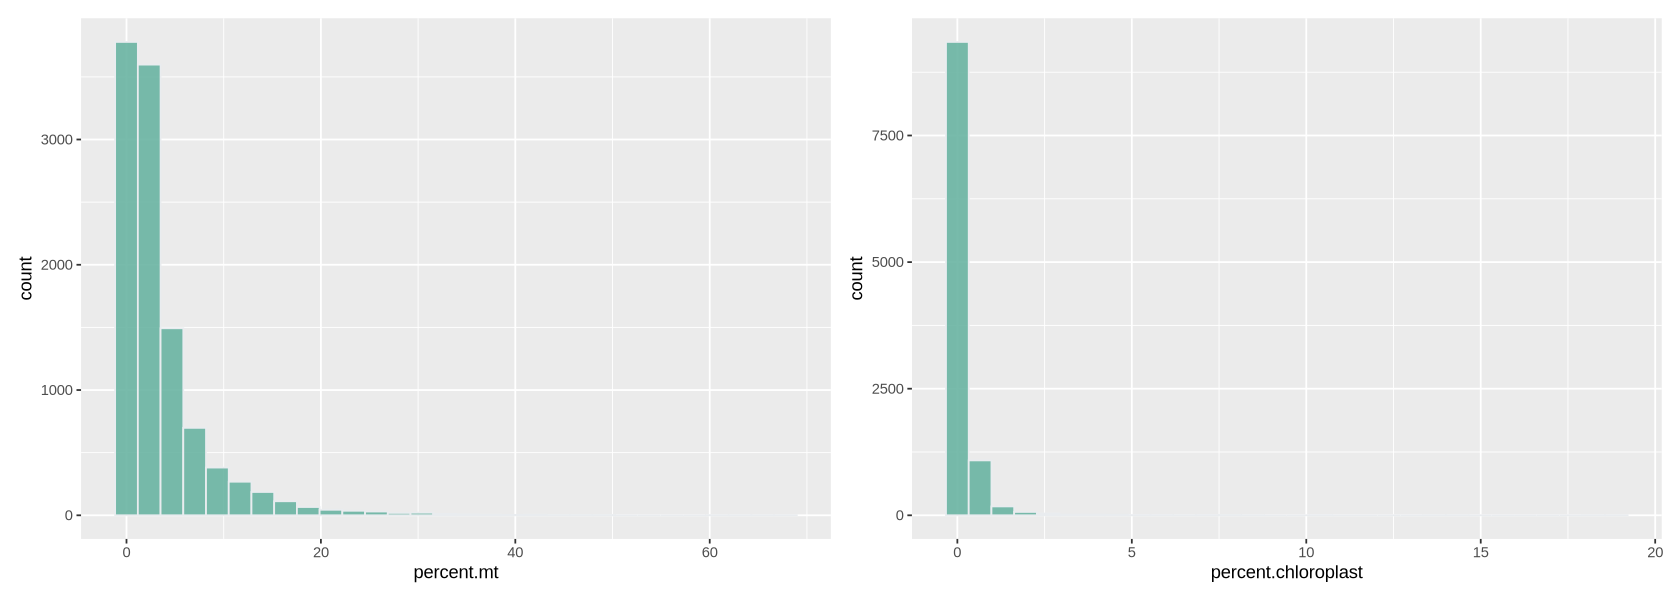
\includegraphics{tutorial-2024_files/figure-pdf/fig-mt-output-2.png}

}

\caption{\label{fig-mt}Histogram of mitochondrial (left) and
chloroplastic (right) percentage of transcripts in each cell}

\end{figure}%

\paragraph{Counts-Features
relationship}\label{counts-features-relationship}

In Figure~\ref{fig-gentra} below, we look at the plot of the number of
transcripts per cell vs the number of detected genes per cell. Usually,
those two measure grow simultaneously. At lower counts the relationship
is quite linear, then becomes a curve, typically bending in favour of
the number of transcripts per cell. You can see below that each dot
(representing a droplet) is coloured by percentage of mitochondria.
Droplets with a high percentage of mitochondrial genes also have very
low amount of transcripts and detected genes, \textbf{confirming that
high mitochondrial content is a measure of low quality}.

\begin{Shaded}
\begin{Highlighting}[]
\FunctionTok{options}\NormalTok{(}\AttributeTok{repr.plot.width=}\DecValTok{14}\NormalTok{, }\AttributeTok{repr.plot.height=}\DecValTok{5}\NormalTok{)}

\NormalTok{meta }\OtherTok{\textless{}{-}}\NormalTok{ Control1\_seurat}\SpecialCharTok{@}\NormalTok{meta.data }\SpecialCharTok{\%\textgreater{}\%} \FunctionTok{arrange}\NormalTok{(percent.mt)}

\NormalTok{plot1 }\OtherTok{\textless{}{-}} \FunctionTok{ggplot}\NormalTok{( meta, }\FunctionTok{aes}\NormalTok{(}\AttributeTok{x=}\NormalTok{nCount\_RNA, }\AttributeTok{y=}\NormalTok{nFeature\_RNA, }\AttributeTok{colour=}\NormalTok{percent.mt)) }\SpecialCharTok{+} 
         \FunctionTok{geom\_point}\NormalTok{(}\AttributeTok{alpha=}\FloatTok{0.75}\NormalTok{, }\AttributeTok{size=}\DecValTok{5}\NormalTok{)}\SpecialCharTok{+}
         \FunctionTok{geom\_smooth}\NormalTok{(}\AttributeTok{se=}\ConstantTok{TRUE}\NormalTok{, }\AttributeTok{method=}\StringTok{"loess"}\NormalTok{)}

\NormalTok{plot1}
\end{Highlighting}
\end{Shaded}

\begin{verbatim}
`geom_smooth()` using formula = 'y ~ x'
Warning message:
“The following aesthetics were dropped during statistical transformation: colour
ℹ This can happen when ggplot fails to infer the correct grouping structure in
  the data.
ℹ Did you forget to specify a `group` aesthetic or to convert a numerical
  variable into a factor?”
\end{verbatim}

\begin{figure}[H]

\centering{

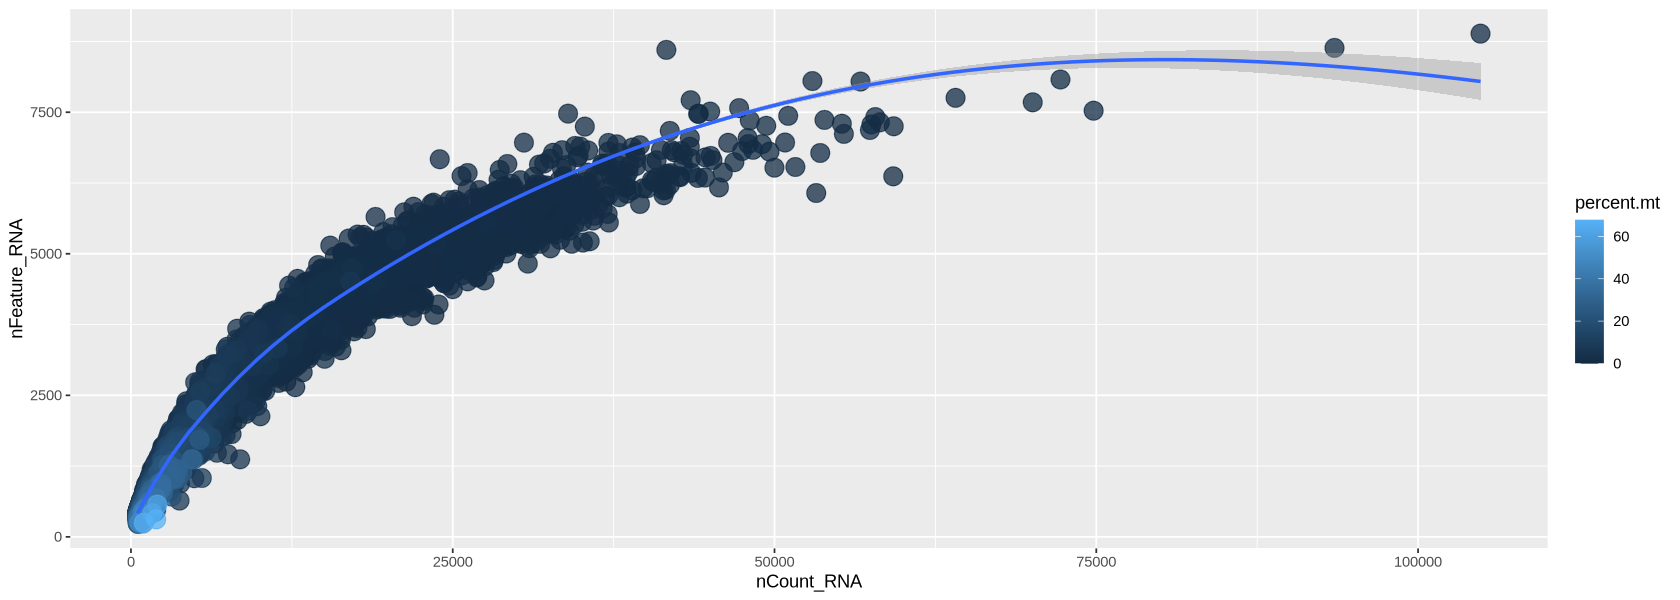
\includegraphics{tutorial-2024_files/figure-pdf/fig-gentra-output-2.png}

}

\caption{\label{fig-gentra}Histogram of the relationship between
detected genes and transcripts per cell, coloured by mitochondrial
content.}

\end{figure}%

In a similar way the chloroplastic genes confirm the pattern of low
quality droplets.

\begin{Shaded}
\begin{Highlighting}[]
\FunctionTok{options}\NormalTok{(}\AttributeTok{repr.plot.width=}\DecValTok{14}\NormalTok{, }\AttributeTok{repr.plot.height=}\DecValTok{5}\NormalTok{)}

\NormalTok{meta }\OtherTok{\textless{}{-}}\NormalTok{ Control1\_seurat}\SpecialCharTok{@}\NormalTok{meta.data }\SpecialCharTok{\%\textgreater{}\%} \FunctionTok{arrange}\NormalTok{(percent.chloroplast)}

\NormalTok{plot1 }\OtherTok{\textless{}{-}} \FunctionTok{ggplot}\NormalTok{( meta, }\FunctionTok{aes}\NormalTok{(}\AttributeTok{x=}\NormalTok{nCount\_RNA, }\AttributeTok{y=}\NormalTok{nFeature\_RNA, }\AttributeTok{colour=}\NormalTok{percent.chloroplast)) }\SpecialCharTok{+} 
         \FunctionTok{geom\_point}\NormalTok{(}\AttributeTok{alpha=}\FloatTok{0.75}\NormalTok{, }\AttributeTok{size=}\DecValTok{5}\NormalTok{)}\SpecialCharTok{+}
         \FunctionTok{geom\_smooth}\NormalTok{(}\AttributeTok{se=}\ConstantTok{TRUE}\NormalTok{, }\AttributeTok{method=}\StringTok{"loess"}\NormalTok{)}

\NormalTok{plot1}
\end{Highlighting}
\end{Shaded}

\begin{verbatim}
`geom_smooth()` using formula = 'y ~ x'
Warning message:
“The following aesthetics were dropped during statistical transformation: colour
ℹ This can happen when ggplot fails to infer the correct grouping structure in
  the data.
ℹ Did you forget to specify a `group` aesthetic or to convert a numerical
  variable into a factor?”
\end{verbatim}

\begin{figure}[H]

\centering{

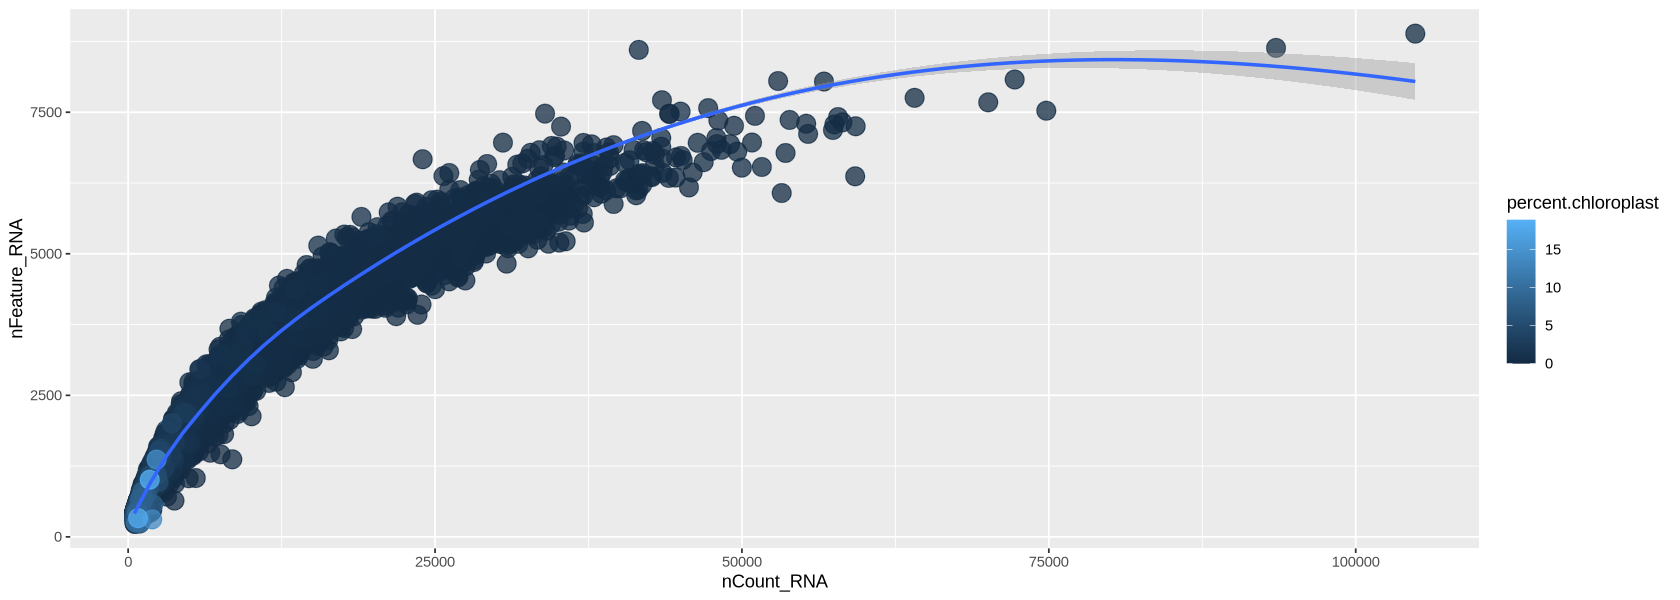
\includegraphics{tutorial-2024_files/figure-pdf/fig-gentrach-output-2.png}

}

\caption{\label{fig-gentrach}Histogram of the relationship between
detected genes and transcripts per cell, coloured by chloroplastic
content.}

\end{figure}%

\subsubsection{Filtering with the chosen
criteria}\label{filtering-with-the-chosen-criteria}

Here we use the command \texttt{subset} and impose the criteria we chose
above looking at the histograms. We set each criteria for keeping cells
of good quality using the names of the features in metadata. We print
those names to remember them.

\begin{Shaded}
\begin{Highlighting}[]
\FunctionTok{cat}\NormalTok{(}\StringTok{"Meta data names:}\SpecialCharTok{\textbackslash{}n}\StringTok{"}\NormalTok{)}
\FunctionTok{cat}\NormalTok{( }\FunctionTok{names}\NormalTok{(Control1\_seurat}\SpecialCharTok{@}\NormalTok{meta.data), }\AttributeTok{sep=}\StringTok{\textquotesingle{}; \textquotesingle{}}\NormalTok{ )}
\end{Highlighting}
\end{Shaded}

\begin{verbatim}
Meta data names:
orig.ident; nCount_RNA; nFeature_RNA; Condition; percent.mt; percent.chloroplast
\end{verbatim}

The filtered object is called \texttt{Control1\_seurat\_filt}

\begin{Shaded}
\begin{Highlighting}[]
\NormalTok{Control1\_seurat\_filt }\OtherTok{\textless{}{-}} \FunctionTok{subset}\NormalTok{(}\AttributeTok{x =}\NormalTok{ Control1\_seurat, }
                                        \AttributeTok{subset =}\NormalTok{ nCount\_RNA }\SpecialCharTok{\textgreater{}} \DecValTok{700} \SpecialCharTok{\&}
\NormalTok{                                                 nCount\_RNA }\SpecialCharTok{\textless{}} \DecValTok{35000} \SpecialCharTok{\&}
\NormalTok{                                                 nFeature\_RNA }\SpecialCharTok{\textgreater{}} \DecValTok{400} \SpecialCharTok{\&} 
\NormalTok{                                                 nFeature\_RNA }\SpecialCharTok{\textless{}} \DecValTok{7000} \SpecialCharTok{\&} 
\NormalTok{                                                 percent.mt }\SpecialCharTok{\textless{}} \DecValTok{5} \SpecialCharTok{\&} 
\NormalTok{                                                 percent.chloroplast }\SpecialCharTok{\textless{}} \DecValTok{5}\NormalTok{)}

\FunctionTok{cat}\NormalTok{(}\StringTok{"Filtered Genes and Cells: "}\NormalTok{)}
\FunctionTok{cat}\NormalTok{( }\FunctionTok{dim}\NormalTok{(Control1\_seurat) }\SpecialCharTok{{-}} \FunctionTok{dim}\NormalTok{(Control1\_seurat\_filt) )}
\FunctionTok{cat}\NormalTok{(}\StringTok{"}\SpecialCharTok{\textbackslash{}n}\StringTok{Remaining Genes and Cells: "}\NormalTok{)}
\FunctionTok{cat}\NormalTok{( }\FunctionTok{dim}\NormalTok{(Control1\_seurat\_filt) )}
\end{Highlighting}
\end{Shaded}

\begin{verbatim}
Filtered Genes and Cells: 0 2762
Remaining Genes and Cells: 23838 8010
\end{verbatim}

Now the transcripts vs genes can be seen in
Figure~\ref{fig-filtrelationship}. The relationship is much more linear
than previously after the removal of extreme values for transcripts and
detected genes.

\begin{Shaded}
\begin{Highlighting}[]
\FunctionTok{options}\NormalTok{(}\AttributeTok{repr.plot.width=}\DecValTok{14}\NormalTok{, }\AttributeTok{repr.plot.height=}\DecValTok{5}\NormalTok{)}

\NormalTok{meta }\OtherTok{\textless{}{-}}\NormalTok{ Control1\_seurat\_filt}\SpecialCharTok{@}\NormalTok{meta.data }\SpecialCharTok{\%\textgreater{}\%} \FunctionTok{arrange}\NormalTok{(percent.mt)}

\NormalTok{plot1 }\OtherTok{\textless{}{-}} \FunctionTok{ggplot}\NormalTok{( meta, }\FunctionTok{aes}\NormalTok{(}\AttributeTok{x=}\NormalTok{nCount\_RNA, }\AttributeTok{y=}\NormalTok{nFeature\_RNA, }\AttributeTok{colour=}\NormalTok{percent.mt)) }\SpecialCharTok{+} 
         \FunctionTok{geom\_point}\NormalTok{(}\AttributeTok{alpha=}\FloatTok{0.75}\NormalTok{, }\AttributeTok{size=}\DecValTok{5}\NormalTok{)}\SpecialCharTok{+}
         \FunctionTok{geom\_smooth}\NormalTok{(}\AttributeTok{se=}\ConstantTok{TRUE}\NormalTok{, }\AttributeTok{method=}\StringTok{"loess"}\NormalTok{)}

\NormalTok{plot1}
\end{Highlighting}
\end{Shaded}

\begin{verbatim}
`geom_smooth()` using formula = 'y ~ x'
Warning message:
“The following aesthetics were dropped during statistical transformation: colour
ℹ This can happen when ggplot fails to infer the correct grouping structure in
  the data.
ℹ Did you forget to specify a `group` aesthetic or to convert a numerical
  variable into a factor?”
\end{verbatim}

\begin{figure}[H]

\centering{

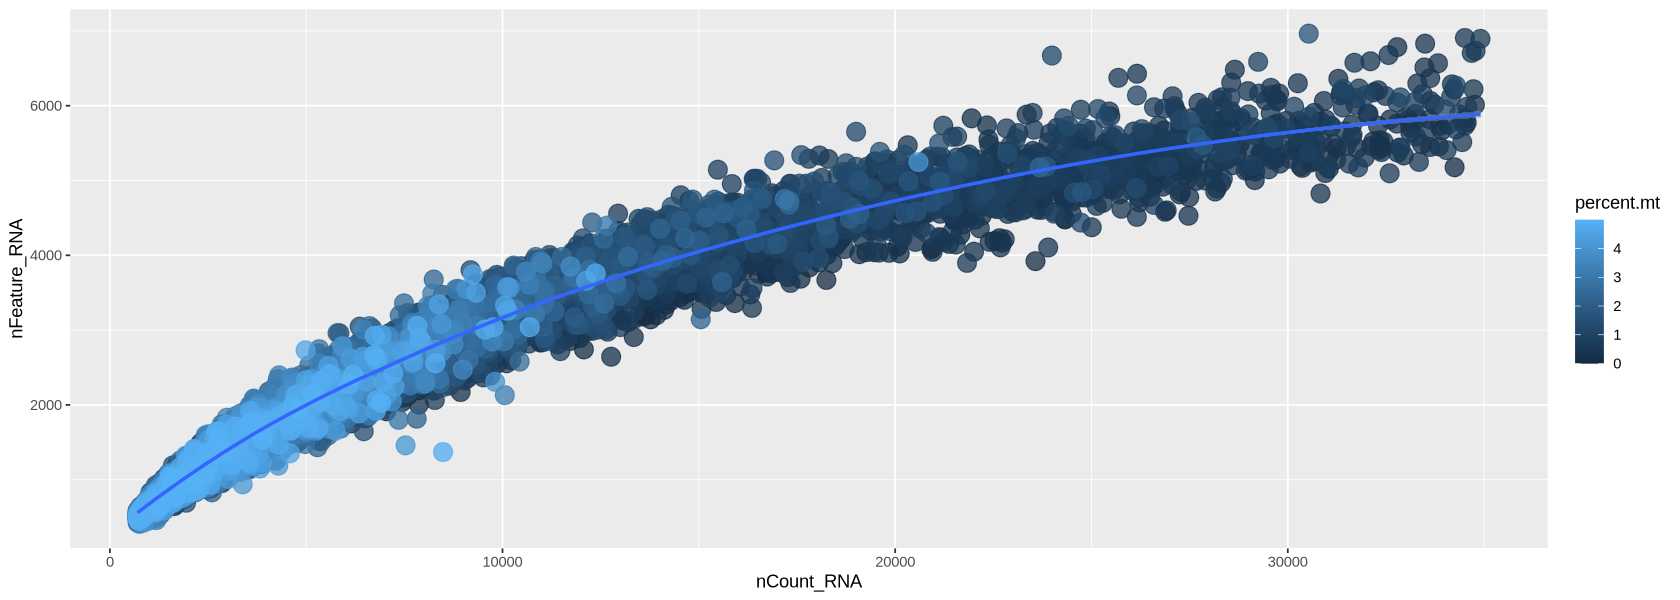
\includegraphics{tutorial-2024_files/figure-pdf/fig-filtrelationship-output-2.png}

}

\caption{\label{fig-filtrelationship}Count vs features after filtering
with the chosen criteria}

\end{figure}%

\subsection{Normalization}\label{normalization}

scRNA-seq data is \textbf{affected by highly variable RNA quantities and
qualities} across different cells. Furthermore, it is often subject to
\textbf{batch effects, sequencing depth differences, and other technical
biases} that can confound downstream analyses.

Normalization methods are used to \textbf{adjust for these technical
variations so that true biological differences between cells can be
accurately identified}.

Some commonly used normalization methods in scRNA-seq data include the
following:

\begin{itemize}
\tightlist
\item
  \textbf{Total count normalization}: Normalizing the read counts to the
  total number of transcripts in each sample
\item
  \textbf{TPM (transcripts per million)} normalization: Normalizing the
  read counts to the total number of transcripts in each sample, scaled
  to a million
\item
  \textbf{Library size normalization:} Normalizing the read counts to
  the total number of reads or transcripts in each sample, adjusted for
  sequencing depth
\end{itemize}

All the above suffer from distorting some gene expressions, especially
if the data varies a lot in term of sequencing depth. A new and more
advanced method, at the moment the state-of-the-art, is
\texttt{SCTransform} (Hafemeister and Satija (2019)), a software package
that can \textbf{correct for technical sources of variation and remove
batch effects}.

\subsubsection{Finding technical sources of
variation}\label{finding-technical-sources-of-variation}

Before normalizing we want to check for technical sources of variation
in the data. One of those is the total number of transcripts: two
similar cells might be sequenced at different depth. This influences of
course normalization. The influence of the number of transcripts per
cell is however always removed by \texttt{SCtransform}.

We want to look into other possible sources of variation. Those are
usually quantities we calculate for each cell, for example the
percentage of mitochondrial and chloroplastic genes.

To see if those quantities actually influence our data a lot, we check
how much is their highest correlation with the first 10 components of
the PCA of the dataset. In short, \textbf{we see if any technical
variation is such that it explains much of the variability of the data,
covering possibly biological signal}.

We now use the function \texttt{plotCorrelations} to plot the highest
correlation of three quantities with the PCA: number of transcripts,
percent of mitochondrial genes and percent of chloroplastic genes. You
will see in Figure~\ref{fig-corr} how \textbf{there is little
correlation for the two percentages}, for which we do not need to worry
about, while \textbf{there is correlation with the total number of
transcripts per cell} (this is always expected and, as mentioned before,
is removed automatically by the normalization process). We created the
function \texttt{plotCorrelations} specifically for the course, together
with a few others, mostly for plotting or handling tables. You can find
them in the file \texttt{script.R}.

\begin{Shaded}
\begin{Highlighting}[]
\FunctionTok{plotCorrelations}\NormalTok{( }\AttributeTok{object=}\NormalTok{Control1\_seurat, }\AttributeTok{measures=}\FunctionTok{c}\NormalTok{(}\StringTok{\textquotesingle{}nCount\_RNA\textquotesingle{}}\NormalTok{, }\StringTok{\textquotesingle{}percent.mt\textquotesingle{}}\NormalTok{, }\StringTok{\textquotesingle{}percent.chloroplast\textquotesingle{}}\NormalTok{) )}
\end{Highlighting}
\end{Shaded}

\begin{verbatim}
`geom_smooth()` using formula = 'y ~ x'
`geom_smooth()` using formula = 'y ~ x'
`geom_smooth()` using formula = 'y ~ x'
\end{verbatim}

\begin{figure}[H]

\centering{

\captionsetup{labelsep=none}

\centering{

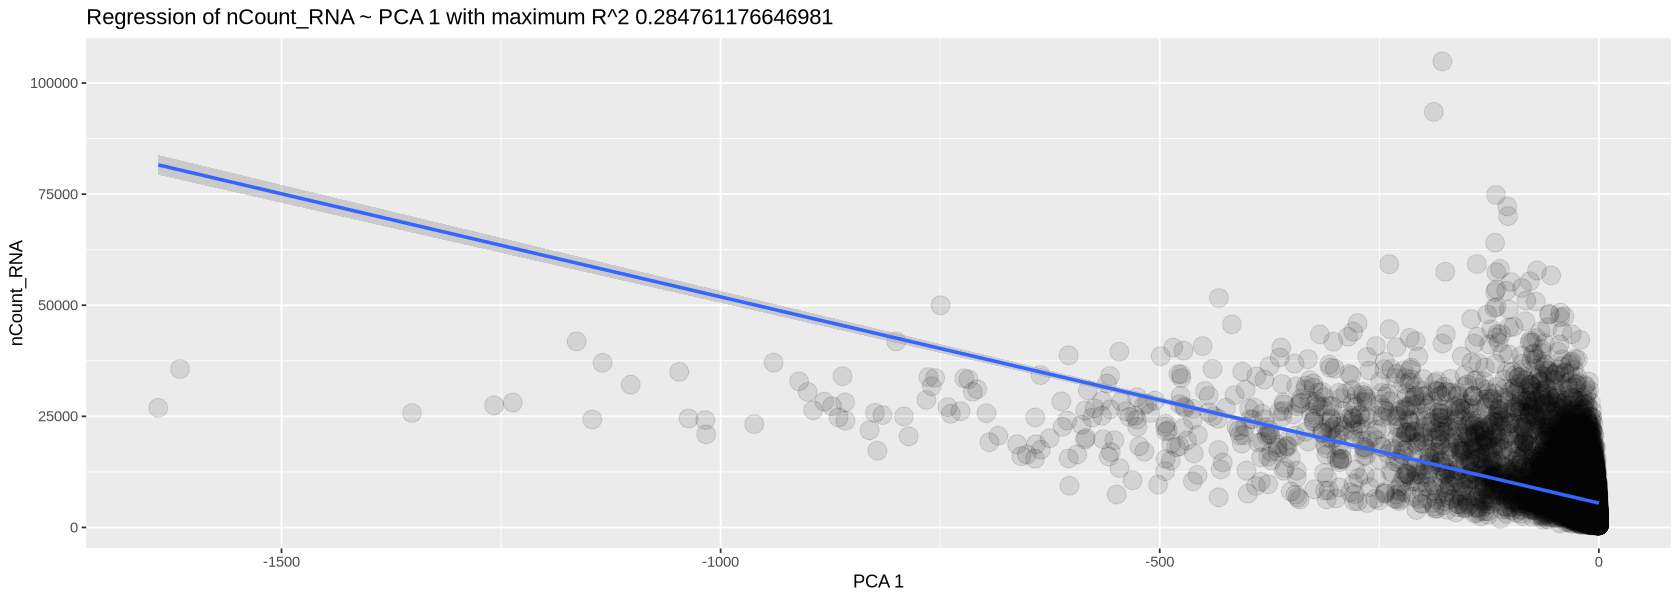
\includegraphics{tutorial-2024_files/figure-pdf/fig-corr-output-2.png}

}

\subcaption{\label{fig-corr-1}Relationships of maximal correlation
between cell quantities and principal components}

\centering{

\captionsetup{labelsep=none}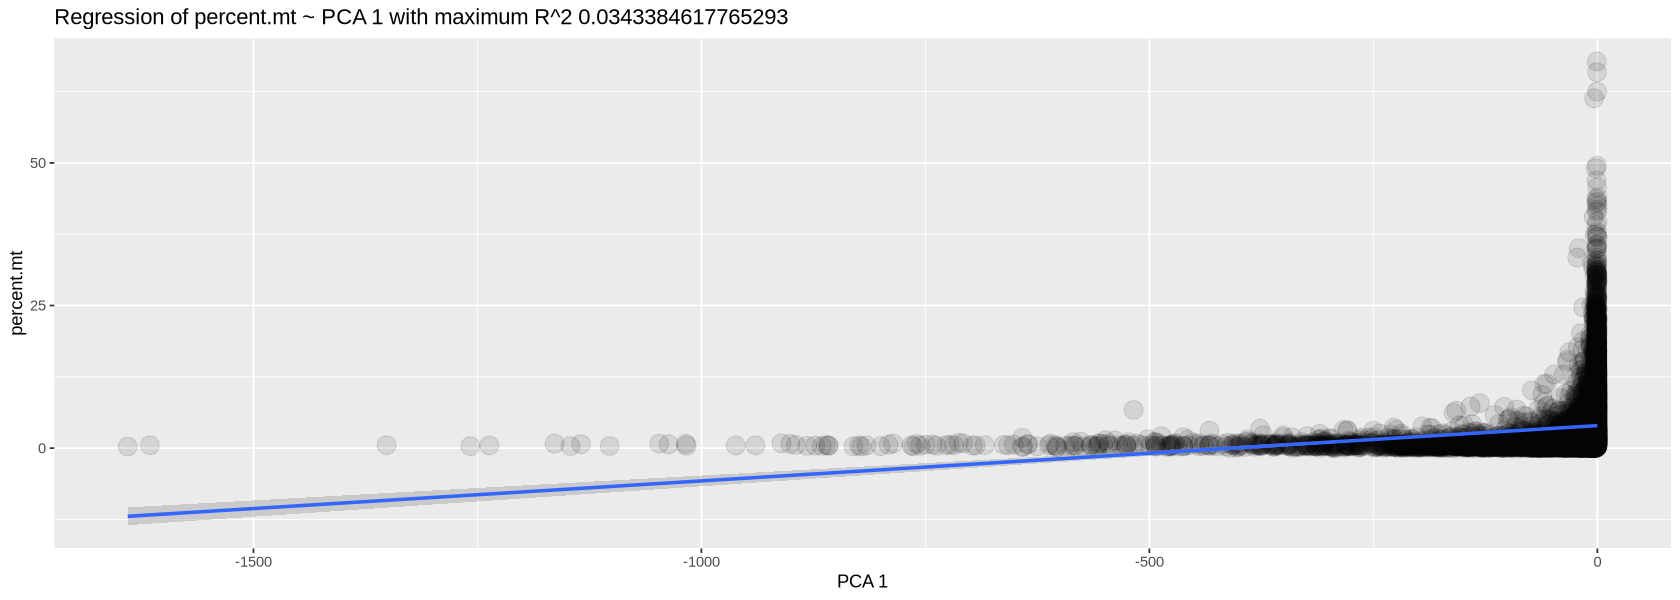
\includegraphics{tutorial-2024_files/figure-pdf/fig-corr-output-3.png}

}

\subcaption{\label{fig-corr-2}}

\centering{

\captionsetup{labelsep=none}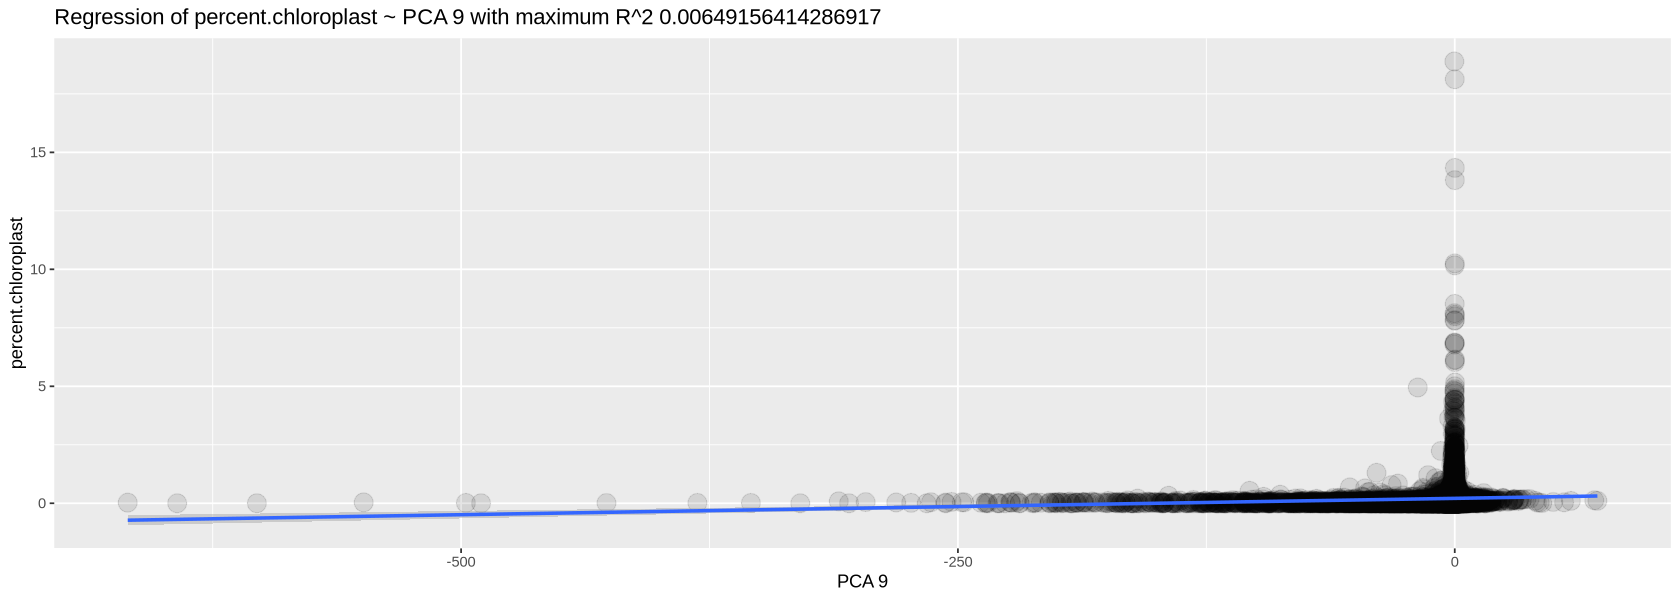
\includegraphics{tutorial-2024_files/figure-pdf/fig-corr-output-4.png}

}

\subcaption{\label{fig-corr-3}}

}

\caption{\label{fig-corr}}

\end{figure}%

\subsubsection{Executing normalization}\label{executing-normalization}

We run \texttt{SCtransform} normalization below. Here you can choose to
subsample some cells to do the normalization (\texttt{ncells} option):
this is \textbf{useful to avoid ending up waiting for a long time}. A
few thousands cells is enough.

You can also choose how many genes to consider for normalization
(\texttt{variable.features.n} option): in this case it is best to
\textbf{use the genes that vary the most their expression across cells}.
We look at a histogram (Figure~\ref{fig-hvg}) of the variance of each
gene to choose a threshold to identify highly-variable genes.

\begin{Shaded}
\begin{Highlighting}[]
\NormalTok{variance\_genes }\OtherTok{\textless{}{-}} \FunctionTok{apply}\NormalTok{( }\FunctionTok{as.matrix}\NormalTok{(Control1\_seurat\_filt[[}\StringTok{\textquotesingle{}RNA\textquotesingle{}}\NormalTok{]]}\SpecialCharTok{@}\NormalTok{counts), }\DecValTok{1}\NormalTok{, var)}

\FunctionTok{options}\NormalTok{(}\AttributeTok{repr.plot.width=}\DecValTok{14}\NormalTok{, }\AttributeTok{repr.plot.height=}\DecValTok{5}\NormalTok{)}

\NormalTok{plot1 }\OtherTok{\textless{}{-}} \FunctionTok{ggplot}\NormalTok{(}\FunctionTok{data.frame}\NormalTok{(variance\_genes), }\FunctionTok{aes}\NormalTok{(variance\_genes)) }\SpecialCharTok{+} 
     \FunctionTok{geom\_histogram}\NormalTok{(}\AttributeTok{fill=}\StringTok{"\#69b3a2"}\NormalTok{, }\AttributeTok{color=}\StringTok{"\#e9ecef"}\NormalTok{, }\AttributeTok{alpha=}\FloatTok{0.9}\NormalTok{) }\SpecialCharTok{+} \FunctionTok{xlim}\NormalTok{(}\DecValTok{0}\NormalTok{,}\DecValTok{1}\NormalTok{)}

\NormalTok{plot1}
\end{Highlighting}
\end{Shaded}

\begin{verbatim}
Warning message in asMethod(object):
“sparse->dense coercion: allocating vector of size 1.4 GiB”
`stat_bin()` using `bins = 30`. Pick better value with `binwidth`.
Warning message:
“Removed 3289 rows containing non-finite values (`stat_bin()`).”
Warning message:
“Removed 2 rows containing missing values (`geom_bar()`).”
\end{verbatim}

\begin{figure}[H]

\centering{

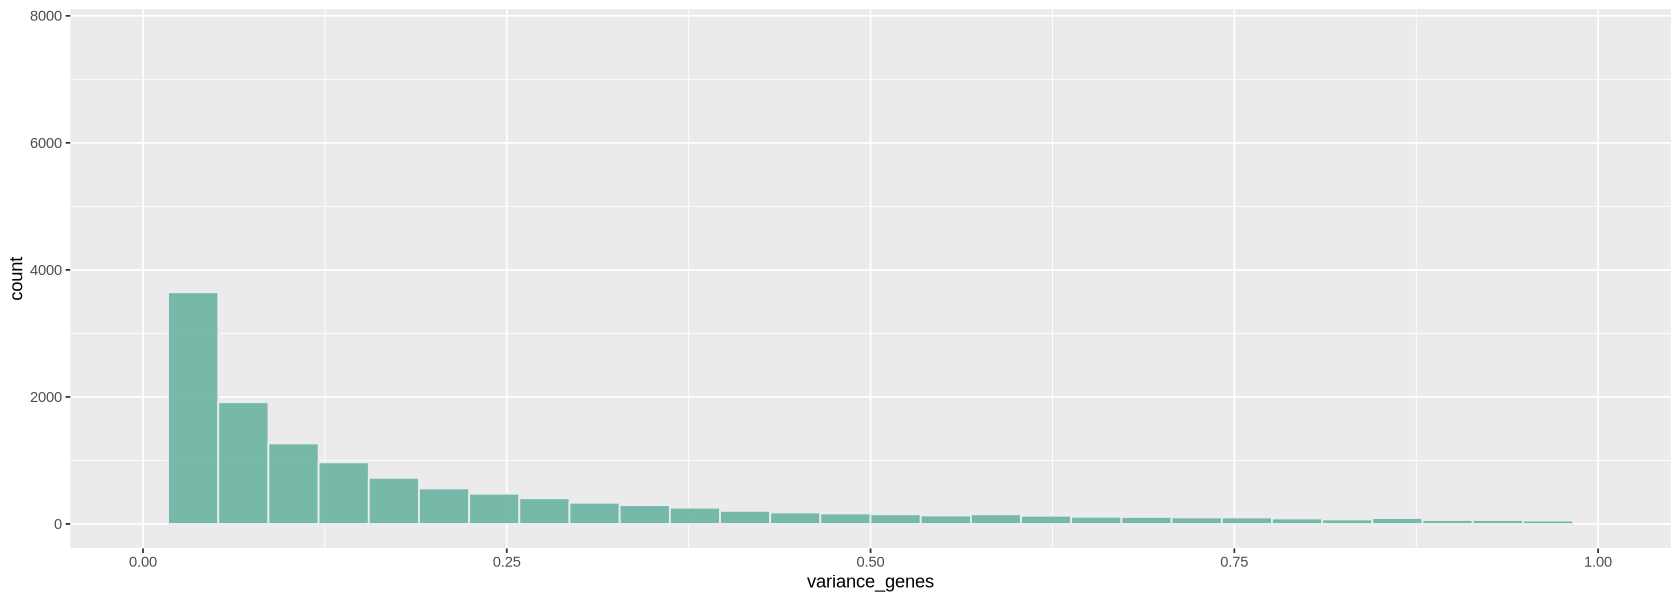
\includegraphics{tutorial-2024_files/figure-pdf/fig-hvg-output-2.png}

}

\caption{\label{fig-hvg}Histogram of genes variance. We choose the
threshold 0.1 to identify highly variable genes.}

\end{figure}%

\begin{Shaded}
\begin{Highlighting}[]
\NormalTok{hvighly\_var\_genes }\OtherTok{\textless{}{-}}\NormalTok{ variance\_genes }\SpecialCharTok{\textgreater{}}\NormalTok{ .}\DecValTok{1}
\FunctionTok{cat}\NormalTok{(}\StringTok{"The total number of highly variable genes selected is: "}\NormalTok{)}
\FunctionTok{cat}\NormalTok{(}\FunctionTok{sum}\NormalTok{( hvighly\_var\_genes ))}
\end{Highlighting}
\end{Shaded}

\begin{verbatim}
The total number of highly variable genes selected is: 9955
\end{verbatim}

\begin{Shaded}
\begin{Highlighting}[]
\NormalTok{Control1\_seurat\_norm }\OtherTok{\textless{}{-}} \FunctionTok{SCTransform}\NormalTok{(Control1\_seurat\_filt, }
                                             \AttributeTok{return.only.var.genes =} \ConstantTok{FALSE}\NormalTok{, }
                                             \AttributeTok{ncells =} \DecValTok{3000}\NormalTok{, }
                                             \AttributeTok{variable.features.n =} \FunctionTok{sum}\NormalTok{( hvighly\_var\_genes ),}
                                             \AttributeTok{verbose =} \ConstantTok{FALSE}\NormalTok{)}
\end{Highlighting}
\end{Shaded}

Normalized data is now in the object \texttt{Control1\_seurat\_norm}, in
a new assay called \texttt{SCT}. This assay is now the default used for
data analysis: you can verify it very easily below:

\begin{Shaded}
\begin{Highlighting}[]
\FunctionTok{cat}\NormalTok{(}\StringTok{"Your default assay is "}\NormalTok{)}
\FunctionTok{cat}\NormalTok{(}\FunctionTok{DefaultAssay}\NormalTok{(}\AttributeTok{object =}\NormalTok{ Control1\_seurat\_norm))}
\end{Highlighting}
\end{Shaded}

\begin{verbatim}
Your default assay is SCT
\end{verbatim}

\subsubsection{Visualizing the result}\label{visualizing-the-result}

Now we plot the UMAP plot of the data to have a first impression of how
the data is structured (presence of clusters, how many, etc.). First of
all, we create a PCA plot, which tells us how many PCA components are of
relevance with the elbow plot of Figure~\ref{fig-elbow}. In the elbow
plot, we see the variability of each component in descending order. Note
how, after a few rapidly descending components, there is an elbow. We
schoose a threshold just after the elbow (for example at 15), which
means those components will be used to calculate some other things of
relevance in the data, such as distance between cells and the UMAP
projection of Figure~\ref{fig-umap}: specific commands using PCA allow
to choose the components, and we will set 10 with the option
\texttt{dims\ =\ 1:15}.

\begin{Shaded}
\begin{Highlighting}[]
\NormalTok{Control1\_seurat\_norm }\OtherTok{\textless{}{-}} \FunctionTok{FindVariableFeatures}\NormalTok{(Control1\_seurat\_norm,}
                                                     \AttributeTok{nfeatures =} \FunctionTok{sum}\NormalTok{( hvighly\_var\_genes ))}
\end{Highlighting}
\end{Shaded}

\begin{Shaded}
\begin{Highlighting}[]
\NormalTok{Control1\_seurat\_norm }\OtherTok{\textless{}{-}} \FunctionTok{RunPCA}\NormalTok{(}\AttributeTok{object =}\NormalTok{ Control1\_seurat\_norm, }
                                        \AttributeTok{verbose =} \ConstantTok{FALSE}\NormalTok{, }\AttributeTok{seed.use =} \DecValTok{123}\NormalTok{)}
\end{Highlighting}
\end{Shaded}

\begin{Shaded}
\begin{Highlighting}[]
\FunctionTok{ElbowPlot}\NormalTok{(Control1\_seurat\_norm, }\AttributeTok{ndims =} \DecValTok{30}\NormalTok{)}
\end{Highlighting}
\end{Shaded}

\begin{figure}[H]

\centering{

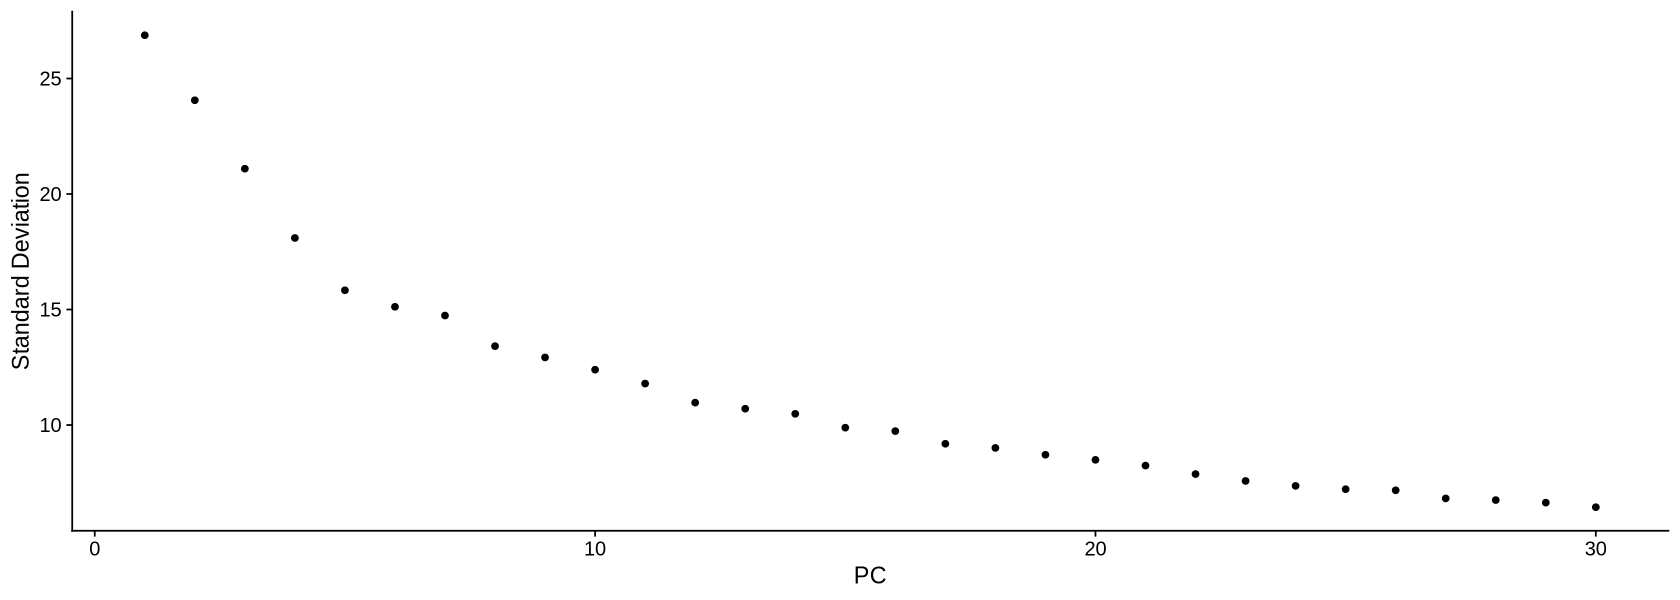
\includegraphics{tutorial-2024_files/figure-pdf/fig-elbow-output-1.png}

}

\caption{\label{fig-elbow}Elbow plot of the first 30 principal
components calculated from the data}

\end{figure}%

We calculate the projection using the UMAP algorithm (McInnes et al.
(2018), Becht et al. (2019)). The parameters \texttt{a} and \texttt{b}
will change how stretched or sparsed the data looks like. When you do
your own UMAP projection, you can avoid setting \texttt{a} and
\texttt{b}, and those will be chosen automatically by the command.

\begin{Shaded}
\begin{Highlighting}[]
\NormalTok{Control1\_seurat\_norm }\OtherTok{\textless{}{-}} \FunctionTok{RunUMAP}\NormalTok{(}\AttributeTok{object =}\NormalTok{ Control1\_seurat\_norm, }
                                         \AttributeTok{a =}\NormalTok{ .}\DecValTok{8}\NormalTok{, }\AttributeTok{b=}\DecValTok{1}\NormalTok{,}
                                         \AttributeTok{dims =} \DecValTok{1}\SpecialCharTok{:}\DecValTok{15}\NormalTok{, }
                                         \AttributeTok{verbose =} \ConstantTok{FALSE}\NormalTok{, }
                                         \AttributeTok{seed.use =} \DecValTok{123}\NormalTok{)}
\end{Highlighting}
\end{Shaded}

\begin{verbatim}
Warning message:
“The default method for RunUMAP has changed from calling Python UMAP via reticulate to the R-native UWOT using the cosine metric
To use Python UMAP via reticulate, set umap.method to 'umap-learn' and metric to 'correlation'
This message will be shown once per session”
Found more than one class "dist" in cache; using the first, from namespace 'spam'

Also defined by ‘BiocGenerics’

Found more than one class "dist" in cache; using the first, from namespace 'spam'

Also defined by ‘BiocGenerics’
\end{verbatim}

In Figure~\ref{fig-umap} we can see the resulting projection. The result
looks pretty neat and structured (we can clearly see there are various
clusters).

\begin{Shaded}
\begin{Highlighting}[]
\FunctionTok{options}\NormalTok{(}\AttributeTok{repr.plot.width=}\DecValTok{10}\NormalTok{, }\AttributeTok{repr.plot.height=}\DecValTok{8}\NormalTok{)}
\FunctionTok{UMAPPlot}\NormalTok{(}\AttributeTok{object =}\NormalTok{ Control1\_seurat\_norm)}
\end{Highlighting}
\end{Shaded}

\begin{figure}[H]

\centering{

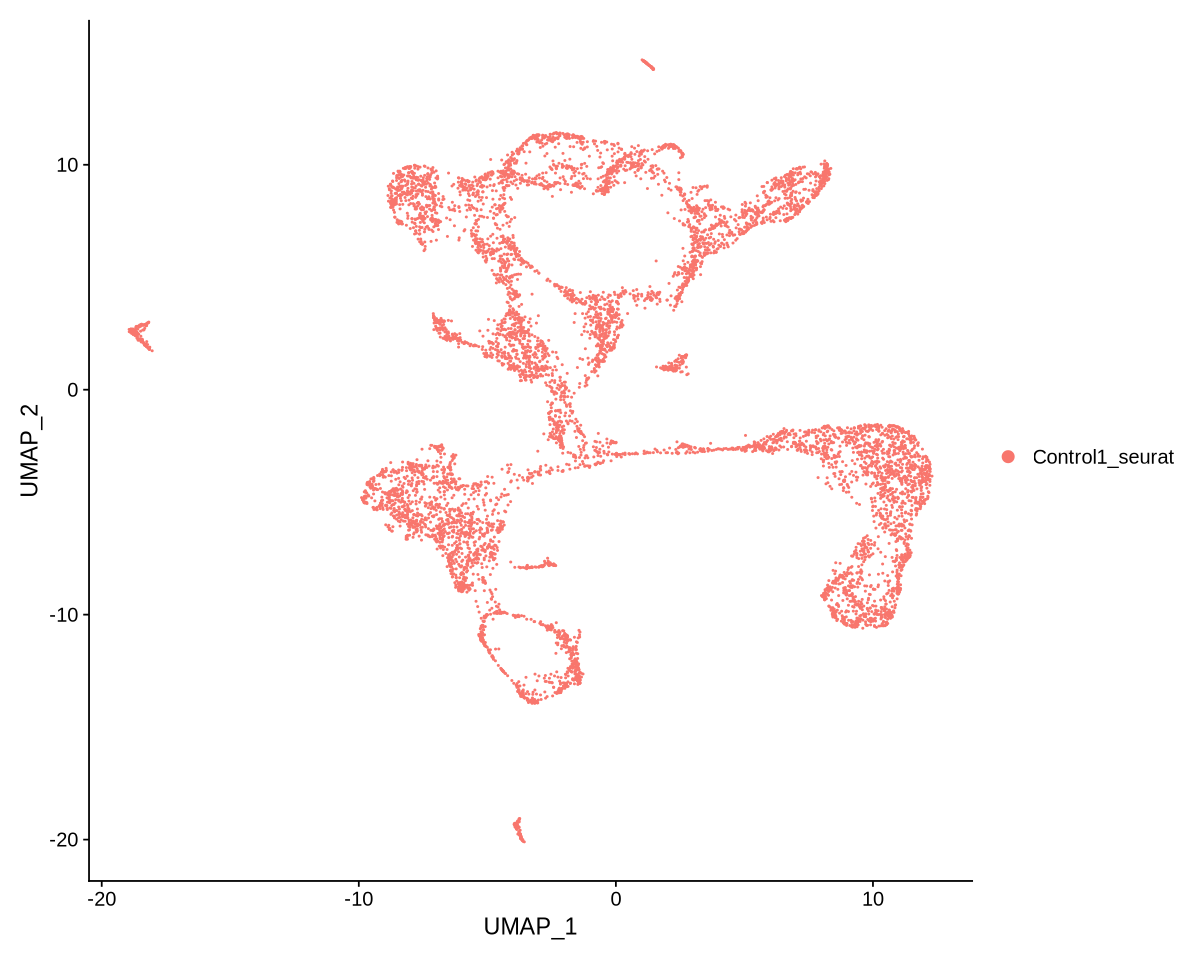
\includegraphics{tutorial-2024_files/figure-pdf/fig-umap-output-1.png}

}

\caption{\label{fig-umap}UMAP projection of the data}

\end{figure}%

\subsection{Removing doublets}\label{removing-doublets}

Doublets removal is part of filtering, but it needs normalized data to
work. This is why we do it after using \texttt{SCtransform}.

Doublets (and the very rare multiplets) refer to droplets that
\textbf{contain the transcriptional profiles of two or more distinct
cells}. Doublets can occur during the cell dissociation process or when
two or more cells are captured in the same droplet during the library
preparation step.

It is quite obvious that a doublet transcriptional profile can confound
downstream analyses, such as cell clustering and differential gene
expression analysis. Most doublet detectors, like \texttt{DoubletFinder}
(McGinnis, Murrow, and Gartner (2019)) which we will use,
\textbf{simulates doublets and then finds cells in the data which are
similar to the simulated doublets}. Most such packages need an idea of
the number/proportion of expected doublets in the dataset. \textbf{As
indicated from the Chromium user guide, expected doublet rates are about
as follows:}

\begin{figure}

\centering{

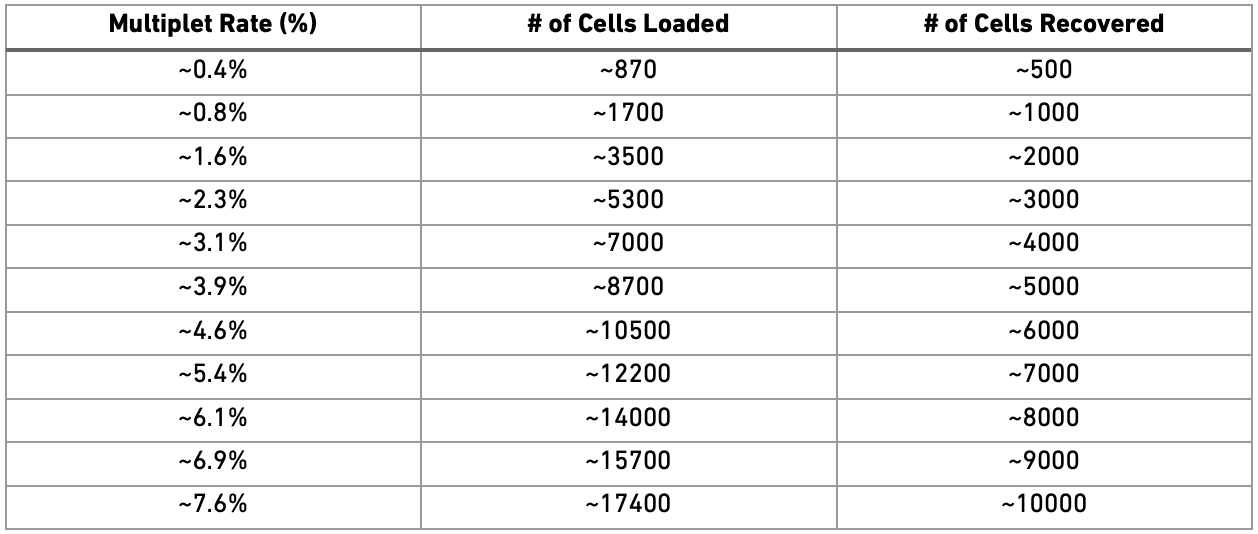
\includegraphics{./images/doublet_rates.png}

}

\caption{\label{fig-doubletrates}Table of expected doublet rates based
on the number of cells.}

\end{figure}%

The data we are using contained about 10000 cells per sample (as in the
knee plot at the beginning), hence we can assume that it originates from
around 18000 loaded cells and should have a doublet rate at about 7.6\%.

\begin{tcolorbox}[enhanced jigsaw, toprule=.15mm, coltitle=black, colframe=quarto-callout-note-color-frame, colback=white, colbacktitle=quarto-callout-note-color!10!white, opacityback=0, arc=.35mm, breakable, rightrule=.15mm, titlerule=0mm, leftrule=.75mm, bottomtitle=1mm, toptitle=1mm, title=\textcolor{quarto-callout-note-color}{\faInfo}\hspace{0.5em}{Note}, bottomrule=.15mm, left=2mm, opacitybacktitle=0.6]

Doublet prediction, like the rest of the filtering, \textbf{should be
run on each sample separately}.

\end{tcolorbox}

Here, we apply \texttt{DoubletFinder} to predict doublet cells. Most
parameters are quite standard, we mostly need to choose \texttt{nExp}
(expected number of doublets), \texttt{PCs} (number of principal
components to use), \texttt{sct} (use the normalized data). The last
three option are not part of the package, but have been added by
creating a slightly modified version
(\href{https://github.com/SamueleSoraggi/DoubletFinder}{here}) - they
allow to use multiple cores and a subset of cells for calculations for a
considerable speedup. However, the code takes some time to run, so be
patient.

\begin{Shaded}
\begin{Highlighting}[]
\NormalTok{nExp }\OtherTok{\textless{}{-}} \FunctionTok{round}\NormalTok{(}\FunctionTok{ncol}\NormalTok{(Control1\_seurat\_norm) }\SpecialCharTok{*} \FloatTok{0.076}\NormalTok{)  }\CommentTok{\# expected doublet rate}
\end{Highlighting}
\end{Shaded}

\begin{Shaded}
\begin{Highlighting}[]
\NormalTok{Control1\_seurat\_norm }\OtherTok{\textless{}{-}} \FunctionTok{doubletFinder\_v3}\NormalTok{(Control1\_seurat\_norm,}
                                                  \AttributeTok{pN =} \FloatTok{0.25}\NormalTok{, }\CommentTok{\#proportion of doublets to simulate)}
                                                  \AttributeTok{pK =} \FloatTok{0.09}\NormalTok{, }
                                                  \AttributeTok{nExp =}\NormalTok{ nExp, }
                                                  \AttributeTok{PCs =} \DecValTok{1}\SpecialCharTok{:}\DecValTok{15}\NormalTok{, }
                                                  \AttributeTok{sct=}\ConstantTok{TRUE}\NormalTok{, }
                                                  \AttributeTok{workers=}\DecValTok{8}\NormalTok{, }
                                                  \AttributeTok{future.globals.maxSize =} \DecValTok{8}\SpecialCharTok{*}\DecValTok{1024}\SpecialCharTok{\^{}}\DecValTok{13}\NormalTok{,}
                                                  \AttributeTok{seurat.ncells=}\DecValTok{3000}\NormalTok{)}
\end{Highlighting}
\end{Shaded}

\begin{verbatim}
Loading required package: fields

Loading required package: spam

Spam version 2.10-0 (2023-10-23) is loaded.
Type 'help( Spam)' or 'demo( spam)' for a short introduction 
and overview of this package.
Help for individual functions is also obtained by adding the
suffix '.spam' to the function name, e.g. 'help( chol.spam)'.


Attaching package: ‘spam’


The following object is masked from ‘package:stats4’:

    mle


The following objects are masked from ‘package:base’:

    backsolve, forwardsolve


Loading required package: viridisLite


Try help(fields) to get started.

Loading required package: KernSmooth

KernSmooth 2.23 loaded
Copyright M. P. Wand 1997-2009

Loading required package: future

Loading required package: sctransform

Calculating cell attributes from input UMI matrix: log_umi

Variance stabilizing transformation of count matrix of size 23388 by 10680

Model formula is y ~ log_umi

Get Negative Binomial regression parameters per gene

Using 2000 genes, 3000 cells

Found 151 outliers - those will be ignored in fitting/regularization step


Second step: Get residuals using fitted parameters for 23388 genes

Computing corrected count matrix for 23388 genes

Calculating gene attributes

Wall clock passed: Time difference of 1.655047 mins

Determine variable features

Place corrected count matrix in counts slot

Centering data matrix

Set default assay to SCT

PC_ 1 
Positive:  LotjaGi2g1v0360900, LotjaGi5g1v0359500, LotjaGi6g1v0155900, LotjaGi6g1v0155800, LotjaGi3g1v0321700, LotjaGi3g1v0414900, LotjaGi3g1v0030500, LotjaGi5g1v0211100, LotjaGi3g1v0506700, LotjaGi4g1v0109600 
       LotjaGi3g1v0009600, LotjaGi1g1v0539300, LotjaGi3g1v0450900, LotjaGi2g1v0269100, LotjaGi3g1v0010900, LotjaGi3g1v0530000, LotjaGi3g1v0373700, LotjaGi4g1v0137700, LotjaGi3g1v0380900, LotjaGi4g1v0309700 
       LotjaGi1g1v0014300, LotjaGi5g1v0359400, LotjaGi6g1v0071000, LotjaGi3g1v0012400, LotjaGi3g1v0162300, LotjaGi3g1v0554100, LotjaGi1g1v0516900, LotjaGi2g1v0316800, LotjaGi2g1v0285600, LotjaGi2g1v0358600 
Negative:  LotjaGi6g1v0254300, LotjaGi3g1v0068000, LotjaGi6g1v0286800-LC, LotjaGi1g1v0080000, LotjaGi5g1v0005800, LotjaGi5g1v0269800-LC, LotjaGi5g1v0293100-LC, LotjaGi3g1v0222100, LotjaGi1g1v0006200, LotjaGi6g1v0254700 
       LotjaGi3g1v0358300, LotjaGi3g1v0329100, LotjaGi3g1v0445300, LotjaGi1g1v0646500-LC, LotjaGi2g1v0157900, LotjaGi3g1v0505900, LotjaGi1g1v0022100, LotjaGi4g1v0076500, LotjaGi4g1v0293000-LC, LotjaGi1g1v0558200 
       LotjaGi1g1v0577100, LotjaGi3g1v0395900-LC, LotjaGi5g1v0031100, LotjaGi5g1v0288600, LotjaGi3g1v0097800, LotjaGi1g1v0261700, LotjaGi4g1v0207600, LotjaGi4g1v0313900, LotjaGi2g1v0303000, LotjaGi1g1v0515200 
PC_ 2 
Positive:  LotjaGi3g1v0358300, LotjaGi6g1v0254300, LotjaGi1g1v0646500-LC, LotjaGi3g1v0038800, LotjaGi6g1v0253800, LotjaGi6g1v0255000, LotjaGi1g1v0006200, LotjaGi6g1v0254700, LotjaGi5g1v0089300, LotjaGi6g1v0022500 
       LotjaGi3g1v0329100, LotjaGi6g1v0043900, LotjaGi1g1v0261700, LotjaGi4g1v0313900, LotjaGi2g1v0303000, LotjaGi5g1v0005800, LotjaGi1g1v0277900, LotjaGi6g1v0022600, LotjaGi4g1v0325700, LotjaGi3g1v0222100 
       LotjaGi1g1v0690000, LotjaGi6g1v0155800, LotjaGi4g1v0293000-LC, LotjaGi2g1v0360900, LotjaGi1g1v0555200, LotjaGi4g1v0284700, LotjaGi3g1v0046800, LotjaGi1g1v0336600, LotjaGi2g1v0239200, LotjaGi2g1v0388100 
Negative:  LotjaGi5g1v0248500, LotjaGi1g1v0405300, LotjaGi1g1v0074900, LotjaGi1g1v0683300, LotjaGi2g1v0160200, LotjaGi4g1v0018700-LC, LotjaGi5g1v0163900, LotjaGi6g1v0315500, LotjaGi6g1v0078500, LotjaGi2g1v0221100 
       LotjaGi2g1v0019900, LotjaGi4g1v0217400, LotjaGi5g1v0248600, LotjaGi4g1v0256800, LotjaGi2g1v0002800-LC, LotjaGi3g1v0204100, LotjaGi2g1v0426500, LotjaGi4g1v0297800, LotjaGi6g1v0246700, LotjaGi1g1v0109100 
       LotjaGi1g1v0109000, LotjaGi3g1v0493400-LC, LotjaGi5g1v0159400, LotjaGi3g1v0086100-LC, LotjaGi5g1v0120700, LotjaGi1g1v0430800-LC, LotjaGi6g1v0292800, LotjaGi1g1v0593900, LotjaGi5g1v0249500, LotjaGi6g1v0216300 
PC_ 3 
Positive:  LotjaGi3g1v0445300, LotjaGi3g1v0505900, LotjaGi1g1v0594900, LotjaGi1g1v0502700, LotjaGi4g1v0275500, LotjaGi1g1v0723600-LC, LotjaGi6g1v0151500, LotjaGi4g1v0208100, LotjaGi5g1v0269800-LC, LotjaGi2g1v0163300 
       LotjaGi6g1v0028000-LC, LotjaGi4g1v0207600, LotjaGi3g1v0115600, LotjaGi1g1v0475000-LC, LotjaGi2g1v0163500, LotjaGi4g1v0207900, LotjaGi1g1v0022100, LotjaGi1g1v0348000, LotjaGi2g1v0176500-LC, LotjaGi2g1v0406200 
       LotjaGi5g1v0266100, LotjaGi2g1v0402200, LotjaGi3g1v0359600, LotjaGi3g1v0506700, LotjaGi6g1v0286800-LC, LotjaGi5g1v0211100, LotjaGi3g1v0414900, LotjaGi4g1v0014800, LotjaGi5g1v0296300-LC, LotjaGi1g1v0659300 
Negative:  LotjaGi1g1v0405300, LotjaGi5g1v0248500, LotjaGi4g1v0018700-LC, LotjaGi1g1v0683300, LotjaGi1g1v0074900, LotjaGi5g1v0163900, LotjaGi3g1v0218300, LotjaGi2g1v0221100, LotjaGi2g1v0019900, LotjaGi6g1v0078500 
       LotjaGi4g1v0217400, LotjaGi4g1v0256800, LotjaGi2g1v0160200, LotjaGi3g1v0204100, LotjaGi3g1v0068000, LotjaGi5g1v0248600, LotjaGi6g1v0253800, LotjaGi3g1v0038800, LotjaGi1g1v0109100, LotjaGi3g1v0493400-LC 
       LotjaGi6g1v0315500, LotjaGi3g1v0086100-LC, LotjaGi3g1v0358300, LotjaGi6g1v0246700, LotjaGi2g1v0002800-LC, LotjaGi5g1v0249500, LotjaGi6g1v0043900, LotjaGi2g1v0426500, LotjaGi2g1v0429600, LotjaGi6g1v0255000 
PC_ 4 
Positive:  LotjaGi5g1v0005800, LotjaGi1g1v0558200, LotjaGi5g1v0288600, LotjaGi3g1v0174100, LotjaGi3g1v0222100, LotjaGi3g1v0068000, LotjaGi2g1v0386600, LotjaGi5g1v0166000-LC, LotjaGi6g1v0286800-LC, LotjaGi3g1v0162600 
       LotjaGi4g1v0121800, LotjaGi3g1v0395900-LC, LotjaGi2g1v0126700, LotjaGi5g1v0099800, LotjaGi4g1v0293000-LC, LotjaGi4g1v0431800, LotjaGi3g1v0178400, LotjaGi1g1v0636800, LotjaGi4g1v0076500, LotjaGi6g1v0012100 
       LotjaGi2g1v0368200, LotjaGi1g1v0393600, LotjaGi1g1v0114400, LotjaGi4g1v0064700, LotjaGi5g1v0003500, LotjaGi1g1v0340500, LotjaGi3g1v0112700, LotjaGi3g1v0191200, LotjaGi6g1v0069200, LotjaGi3g1v0192300 
Negative:  LotjaGi5g1v0269800-LC, LotjaGi5g1v0120700, LotjaGi3g1v0420400, LotjaGi2g1v0157900, LotjaGi1g1v0377600, LotjaGi6g1v0253800, LotjaGi6g1v0254700, LotjaGi5g1v0293100-LC, LotjaGi1g1v0613100, LotjaGi1g1v0646500-LC 
       LotjaGi1g1v0022100, LotjaGi2g1v0303000, LotjaGi3g1v0055400, LotjaGi2g1v0176500-LC, LotjaGi5g1v0119900, LotjaGi1g1v0515200, LotjaGi2g1v0163500, LotjaGi3g1v0445300, LotjaGi3g1v0420800, LotjaGi3g1v0046800 
       LotjaGi3g1v0115400, LotjaGi3g1v0505900, LotjaGi1g1v0723600-LC, LotjaGi1g1v0690000, LotjaGi1g1v0475000-LC, LotjaGi4g1v0207600, LotjaGi3g1v0329100, LotjaGi1g1v0277900, LotjaGi4g1v0060000, LotjaGi3g1v0420000 
PC_ 5 
Positive:  LotjaGi3g1v0328800, LotjaGi3g1v0222100, LotjaGi4g1v0417500, LotjaGi3g1v0328900, LotjaGi2g1v0450600, LotjaGi3g1v0201800, LotjaGi4g1v0293000-LC, LotjaGi3g1v0378600, LotjaGi5g1v0166000-LC, LotjaGi1g1v0353400 
       LotjaGi3g1v0395900-LC, LotjaGi6g1v0069200, LotjaGi6g1v0155800, LotjaGi6g1v0286800-LC, LotjaGi3g1v0546100, LotjaGi3g1v0445300, LotjaGi6g1v0326300, LotjaGi3g1v0162300, LotjaGi5g1v0288600, LotjaGi5g1v0031100 
       LotjaGi1g1v0601700, LotjaGi3g1v0174100, LotjaGi1g1v0594900, LotjaGi5g1v0266100, LotjaGi3g1v0505900, LotjaGi4g1v0284700, LotjaGi1g1v0393600, LotjaGi6g1v0043900, LotjaGi4g1v0269400, LotjaGi1g1v0795300 
Negative:  LotjaGi4g1v0121800, LotjaGi3g1v0068000, LotjaGi5g1v0099800, LotjaGi3g1v0178400, LotjaGi2g1v0368200, LotjaGi6g1v0012100, LotjaGi1g1v0114400, LotjaGi2g1v0452500, LotjaGi1g1v0240900-LC, LotjaGi5g1v0003500 
       LotjaGi3g1v0192300, LotjaGi2g1v0301500, LotjaGi4g1v0300800-LC, LotjaGi3g1v0162600, LotjaGi5g1v0120700, LotjaGi5g1v0102500, LotjaGi4g1v0298100, LotjaGi5g1v0100000, LotjaGi3g1v0506700, LotjaGi2g1v0345700 
       LotjaGi1g1v0137600, LotjaGi3g1v0001800, LotjaGi1g1v0760600, LotjaGi5g1v0094100, LotjaGi1g1v0221300, LotjaGi4g1v0431800, LotjaGi4g1v0455200, LotjaGi6g1v0232200, LotjaGi4g1v0064700, LotjaGi1g1v0300600 
\end{verbatim}

\begin{verbatim}
[1] "Creating 2670 artificial doublets..."
[1] "Creating Seurat object..."
[1] "Running SCTransform..."
  |======================================================================| 100%
  |======================================================================| 100%
  |======================================================================| 100%
[1] "Running PCA..."
[1] "Calculating PC distance matrix..."
[1] "Computing pANN..."
[1] "Classifying doublets.."
\end{verbatim}

We visualize the UMAP plot and which cells are estimated doublets in
Figure~\ref{fig-doublets}. Fortunately, there are only a few to discard.

\begin{Shaded}
\begin{Highlighting}[]
\FunctionTok{options}\NormalTok{(}\AttributeTok{repr.plot.width=}\DecValTok{10}\NormalTok{, }\AttributeTok{repr.plot.height=}\DecValTok{10}\NormalTok{)}

\NormalTok{DF.name }\OtherTok{=} \FunctionTok{colnames}\NormalTok{(Control1\_seurat\_norm}\SpecialCharTok{@}\NormalTok{meta.data)[}\FunctionTok{grepl}\NormalTok{(}\StringTok{"DF.classification"}\NormalTok{, }\FunctionTok{colnames}\NormalTok{(Control1\_seurat\_norm}\SpecialCharTok{@}\NormalTok{meta.data))]}

\FunctionTok{DimPlot}\NormalTok{(Control1\_seurat\_norm, }\AttributeTok{group.by =}\NormalTok{ DF.name, }\AttributeTok{pt.size =} \DecValTok{2}\NormalTok{, }
        \AttributeTok{split.by =}\NormalTok{ DF.name)}
\end{Highlighting}
\end{Shaded}

\begin{figure}[H]

\centering{

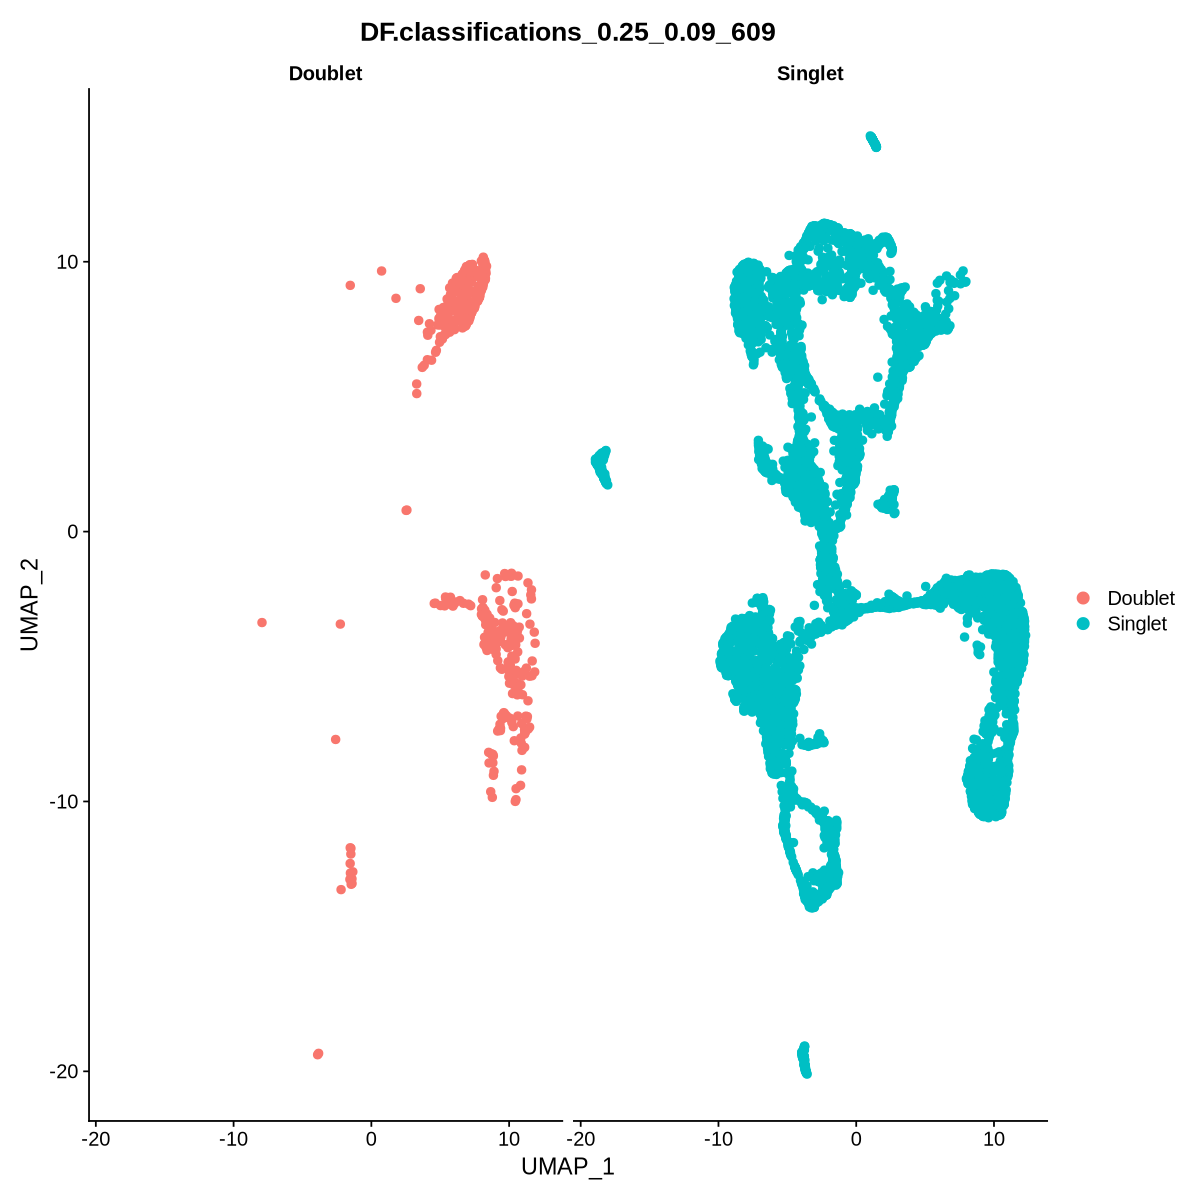
\includegraphics{tutorial-2024_files/figure-pdf/fig-doublets-output-1.png}

}

\caption{\label{fig-doublets}UMAP projection of the data coloured by
doublet or singlet label}

\end{figure}%

Sometimes doublets have more detected genes than a single cell. In our
case, some of the droplets have higher number of genes than the average
(the red violin is large also above 3000 detected genes), so there is
aclear sign of the presence of some doublets. Of course, as with any
filtering, we might remove some actual cells. To be more effective in
our filtering, we can select doublets with more than 2000 detected genes
when we filter.

\begin{Shaded}
\begin{Highlighting}[]
\FunctionTok{VlnPlot}\NormalTok{(Control1\_seurat\_norm, }\AttributeTok{features =} \StringTok{"nFeature\_RNA"}\NormalTok{, }\AttributeTok{group.by =}\NormalTok{ DF.name, }\AttributeTok{pt.size =} \FloatTok{0.1}\NormalTok{)}
\end{Highlighting}
\end{Shaded}

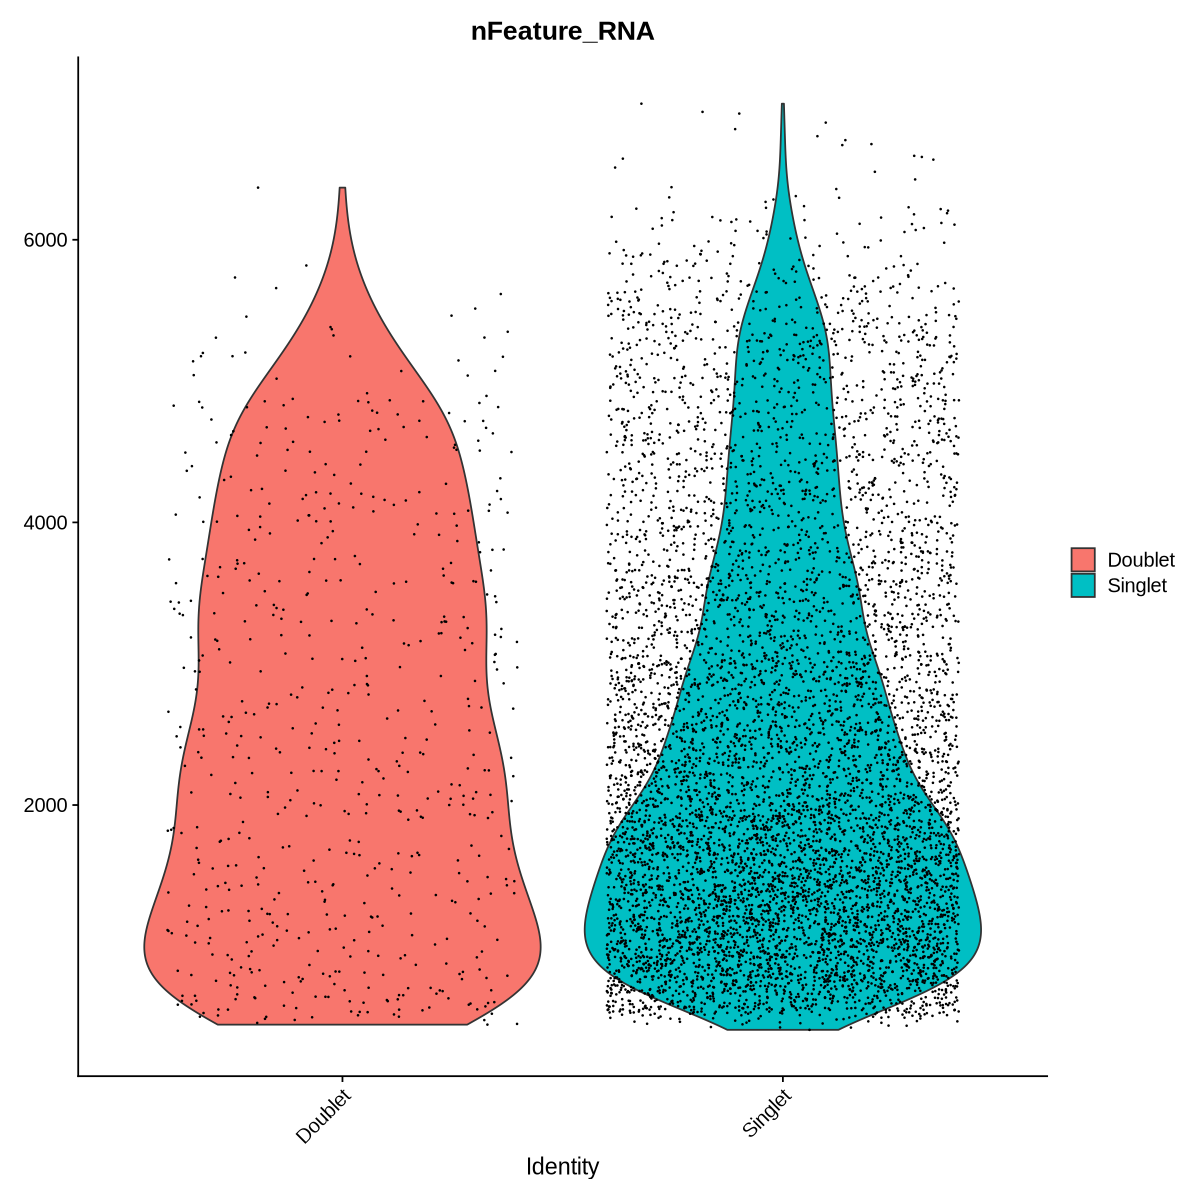
\includegraphics{tutorial-2024_files/figure-pdf/cell-42-output-1.png}

Here we keep only singlets:

\begin{Shaded}
\begin{Highlighting}[]
\NormalTok{Control1\_seurat\_norm }\OtherTok{=}\NormalTok{ Control1\_seurat\_norm[, (Control1\_seurat\_norm}\SpecialCharTok{@}\NormalTok{meta.data[, DF.name] }\SpecialCharTok{==} \StringTok{"Singlet"}\NormalTok{)}\SpecialCharTok{\&}\NormalTok{(Control1\_seurat\_norm}\SpecialCharTok{@}\NormalTok{meta.data}\SpecialCharTok{$}\NormalTok{nFeature\_RNA}\SpecialCharTok{\textgreater{}}\DecValTok{2000}\NormalTok{)]}
\end{Highlighting}
\end{Shaded}

We save our data after all the filtering work!

\begin{Shaded}
\begin{Highlighting}[]
\FunctionTok{SaveH5Seurat}\NormalTok{(}\AttributeTok{object =}\NormalTok{ Control1\_seurat\_norm, }
             \AttributeTok{filename =} \StringTok{"control1.normalized.h5Seurat"}\NormalTok{, }
             \AttributeTok{overwrite =} \ConstantTok{TRUE}\NormalTok{,}
             \AttributeTok{verbose =} \ConstantTok{FALSE}\NormalTok{)}
\end{Highlighting}
\end{Shaded}

\begin{verbatim}
Warning message:
“Overwriting previous file control1.normalized.h5Seurat”
Creating h5Seurat file for version 3.1.5.9900
\end{verbatim}

\section{Integration}\label{sec-integration}

Integration of scRNA-seq data is useful to combine datasets from
different experimental conditions (in our case the Control vs Infected)
and sequencing runs, to gain a broader understanding of cellular
processes. Integration is challenging due to technical variations and
biological differences between the datasets (where we want to remove the
formers to study correctly the latters).

Before integrating scRNA-seq datasets, we have applyed \textbf{quality
control and normalization to each sample} to ensure consistency and
accuracy of the data. Integration can happen using various methods
(Adossa et al. (2021)). Seurat uses \textbf{canonical correlation
analysis (CCA)} (Stuart et al. (2019), Xinming (2022)) to integrate
scRNA-seq datasets from different experimental conditions. CCA
identifies shared variation between two datasets while accounting for
technical differences, such as batch effects.

The shared covariance patterns \textbf{can represent biological signals
that are common across the datasets}, such as cell types or signaling
pathways.

We load another control and two infected datasets. Those have been
previously preprocessed, so you will not need to. Remember again: each
dataset must be preprocessed separately before integration.

\begin{Shaded}
\begin{Highlighting}[]
\NormalTok{Control1\_seurat\_norm }\OtherTok{\textless{}{-}} \FunctionTok{LoadH5Seurat}\NormalTok{(}\StringTok{"control1.normalized.h5Seurat"}\NormalTok{, }\AttributeTok{verbose =} \ConstantTok{FALSE}\NormalTok{)}
\end{Highlighting}
\end{Shaded}

\begin{verbatim}
Validating h5Seurat file
\end{verbatim}

\begin{Shaded}
\begin{Highlighting}[]
\NormalTok{Control2\_seurat\_norm }\OtherTok{\textless{}{-}} \FunctionTok{LoadH5Seurat}\NormalTok{(}\StringTok{"../Data/control2.normalized.h5Seurat"}\NormalTok{, }\AttributeTok{verbose =} \ConstantTok{FALSE}\NormalTok{)}
\NormalTok{Infected1\_seurat\_norm }\OtherTok{\textless{}{-}} \FunctionTok{LoadH5Seurat}\NormalTok{(}\StringTok{"../Data/infected1.normalized.h5Seurat"}\NormalTok{, }\AttributeTok{verbose =} \ConstantTok{FALSE}\NormalTok{)}
\NormalTok{Infected2\_seurat\_norm }\OtherTok{\textless{}{-}} \FunctionTok{LoadH5Seurat}\NormalTok{(}\StringTok{"../Data/infected2.normalized.h5Seurat"}\NormalTok{, }\AttributeTok{verbose =} \ConstantTok{FALSE}\NormalTok{)}
\end{Highlighting}
\end{Shaded}

\begin{verbatim}
Validating h5Seurat file

Validating h5Seurat file

Validating h5Seurat file
\end{verbatim}

To integrate the datasets, we need to start creating a list with all
datasets.

\begin{Shaded}
\begin{Highlighting}[]
\NormalTok{Gifu.list }\OtherTok{\textless{}{-}} \FunctionTok{list}\NormalTok{(Control1\_seurat\_norm, }
\NormalTok{                  Control2\_seurat\_norm, }
\NormalTok{                  Infected1\_seurat\_norm, }
\NormalTok{                  Infected2\_seurat\_norm)}
\end{Highlighting}
\end{Shaded}

We then start by normalizing each dataset of the list with
\texttt{SCtransform}. Here we also have a commented command (with the
symbol \texttt{\#}) that is not executed, to show how you add technical
variations to be removed with the option \texttt{vars.to.regress}, if
necessary (this is not the case of the tutorial).

\begin{Shaded}
\begin{Highlighting}[]
\NormalTok{Gifu.list }\OtherTok{\textless{}{-}} \FunctionTok{lapply}\NormalTok{(}\AttributeTok{X =}\NormalTok{ Gifu.list, }\AttributeTok{FUN =} \ControlFlowTok{function}\NormalTok{(x) \{}
  \FunctionTok{message}\NormalTok{(}\StringTok{"Normalizing}\SpecialCharTok{\textbackslash{}n}\StringTok{"}\NormalTok{)}
  \CommentTok{\#x \textless{}{-} SCTransform(x, vars.to.regress = c("percent.mt",  "percent.chloroplast"), variable.features.n = 10000, return.only.var.genes = FALSE, verbose = TRUE)}
\NormalTok{  x }\OtherTok{\textless{}{-}} \FunctionTok{SCTransform}\NormalTok{(x, }\AttributeTok{ncells=}\DecValTok{3000}\NormalTok{, }\AttributeTok{variable.features.n =} \DecValTok{10000}\NormalTok{, }\AttributeTok{return.only.var.genes =} \ConstantTok{FALSE}\NormalTok{, }\AttributeTok{verbose=}\ConstantTok{FALSE}\NormalTok{)}
\NormalTok{\})}
\end{Highlighting}
\end{Shaded}

\begin{verbatim}
Normalizing


Normalizing


Normalizing


Normalizing

\end{verbatim}

Now we apply the CCA (Canonical Correlation Analysis) to put datasets
together according to their similarities, while removing differences.
The number of genes to use during integration is expressed below as
\texttt{nfeatures}. We choose a reasonable number of features, for
example 10000, which is similar to what we used in the normalization
steps along the tutorial.

\begin{Shaded}
\begin{Highlighting}[]
\NormalTok{Gifu.features }\OtherTok{\textless{}{-}} \FunctionTok{SelectIntegrationFeatures}\NormalTok{(}\AttributeTok{object.list =}\NormalTok{ Gifu.list, }\AttributeTok{nfeatures =} \DecValTok{10000}\NormalTok{)}

\NormalTok{Gifu.list }\OtherTok{\textless{}{-}} \FunctionTok{PrepSCTIntegration}\NormalTok{(}\AttributeTok{object.list =}\NormalTok{ Gifu.list, }\AttributeTok{anchor.features =}\NormalTok{ Gifu.features)}
\end{Highlighting}
\end{Shaded}

\begin{Shaded}
\begin{Highlighting}[]
\NormalTok{Gifu.anchors }\OtherTok{\textless{}{-}} \FunctionTok{FindIntegrationAnchors}\NormalTok{(}\AttributeTok{object.list =}\NormalTok{ Gifu.list, }\AttributeTok{normalization.method =} \StringTok{"SCT"}\NormalTok{, }
                                       \AttributeTok{anchor.features =}\NormalTok{ Gifu.features, }\AttributeTok{reference =} \FunctionTok{c}\NormalTok{(}\DecValTok{1}\NormalTok{,}\DecValTok{2}\NormalTok{))}

\NormalTok{seurat.integrated }\OtherTok{\textless{}{-}} \FunctionTok{IntegrateData}\NormalTok{(}\AttributeTok{anchorset =}\NormalTok{ Gifu.anchors, }\AttributeTok{normalization.method =} \StringTok{"SCT"}\NormalTok{)}
\end{Highlighting}
\end{Shaded}

\begin{verbatim}
Warning message in CheckDuplicateCellNames(object.list = object.list):
“Some cell names are duplicated across objects provided. Renaming to enforce unique cell names.”
Finding anchors between all query and reference datasets

Running CCA

Merging objects

Finding neighborhoods

Finding anchors

    Found 8777 anchors

Filtering anchors

    Retained 8517 anchors

Running CCA

Merging objects

Finding neighborhoods

Finding anchors

    Found 8962 anchors

Filtering anchors

    Retained 8046 anchors

Running CCA

Merging objects

Finding neighborhoods

Finding anchors

    Found 10128 anchors

Filtering anchors

    Retained 9486 anchors

Running CCA

Merging objects

Finding neighborhoods

Finding anchors

    Found 7768 anchors

Filtering anchors

    Retained 7424 anchors

Running CCA

Merging objects

Finding neighborhoods

Finding anchors

    Found 8694 anchors

Filtering anchors

    Retained 8493 anchors

Building integrated reference

Merging dataset 1 into 2

Extracting anchors for merged samples

Finding integration vectors

Finding integration vector weights

Integrating data


Integrating dataset 3 with reference dataset

Finding integration vectors

Finding integration vector weights

Integrating data

Warning message:
“UNRELIABLE VALUE: One of the ‘future.apply’ iterations (‘future_lapply-1’) unexpectedly generated random numbers without declaring so. There is a risk that those random numbers are not statistically sound and the overall results might be invalid. To fix this, specify 'future.seed=TRUE'. This ensures that proper, parallel-safe random numbers are produced via the L'Ecuyer-CMRG method. To disable this check, use 'future.seed = NULL', or set option 'future.rng.onMisuse' to "ignore".”

Integrating dataset 4 with reference dataset

Finding integration vectors

Finding integration vector weights

Integrating data

Warning message:
“UNRELIABLE VALUE: One of the ‘future.apply’ iterations (‘future_lapply-2’) unexpectedly generated random numbers without declaring so. There is a risk that those random numbers are not statistically sound and the overall results might be invalid. To fix this, specify 'future.seed=TRUE'. This ensures that proper, parallel-safe random numbers are produced via the L'Ecuyer-CMRG method. To disable this check, use 'future.seed = NULL', or set option 'future.rng.onMisuse' to "ignore".”
\end{verbatim}

Now the default assay used for analysis has changed into
\texttt{integrated}:

\begin{Shaded}
\begin{Highlighting}[]
\FunctionTok{cat}\NormalTok{(}\StringTok{"The default assay of the data is now called: "}\NormalTok{)}
\FunctionTok{cat}\NormalTok{(}\FunctionTok{DefaultAssay}\NormalTok{(seurat.integrated))}
\end{Highlighting}
\end{Shaded}

\begin{verbatim}
The default assay of the data is now called: integrated
\end{verbatim}

We need to recalculate PCA and UMAP to look at all datasets integrated
together. We choose again 10 principal components from
Figure~\ref{fig-elbowint}. The newUMAP is in Figure~\ref{fig-umapint}.

\begin{Shaded}
\begin{Highlighting}[]
\NormalTok{seurat.integrated }\OtherTok{\textless{}{-}} \FunctionTok{RunPCA}\NormalTok{(}\AttributeTok{object =}\NormalTok{ seurat.integrated, }\AttributeTok{verbose =} \ConstantTok{FALSE}\NormalTok{)}
\end{Highlighting}
\end{Shaded}

\begin{Shaded}
\begin{Highlighting}[]
\FunctionTok{ElbowPlot}\NormalTok{(seurat.integrated, }\AttributeTok{ndims =} \DecValTok{30}\NormalTok{)}
\end{Highlighting}
\end{Shaded}

\begin{figure}[H]

\centering{

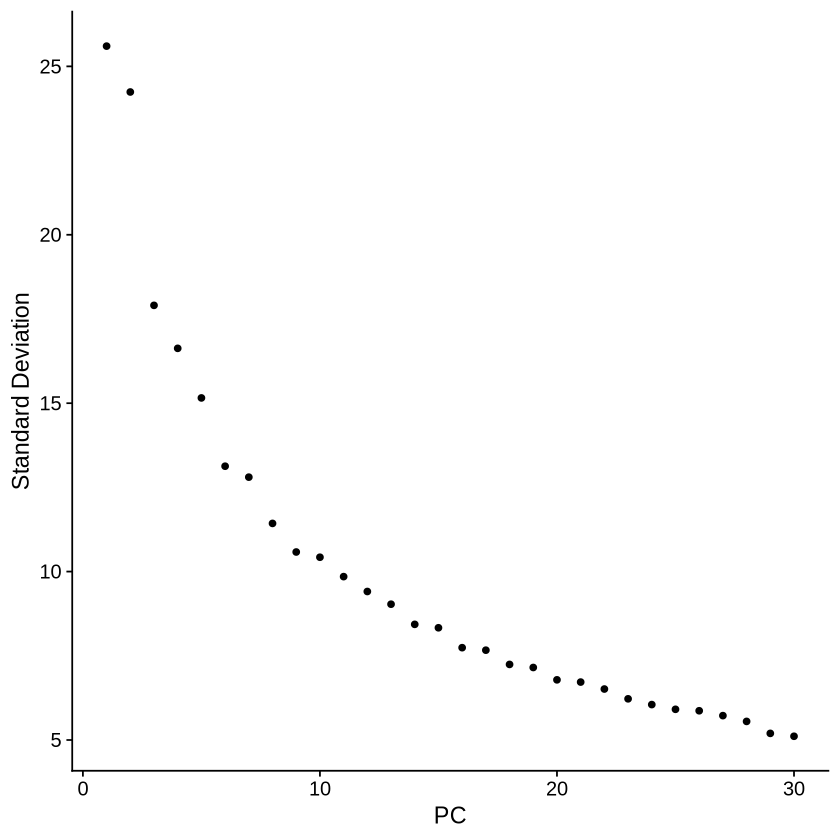
\includegraphics{tutorial-2024_files/figure-pdf/fig-elbowint-output-1.png}

}

\caption{\label{fig-elbowint}Elbow plot of integrated datasets}

\end{figure}%

\begin{Shaded}
\begin{Highlighting}[]
\NormalTok{seurat.integrated }\OtherTok{\textless{}{-}} \FunctionTok{FindNeighbors}\NormalTok{(}\AttributeTok{object =}\NormalTok{ seurat.integrated, }\AttributeTok{dims =} \DecValTok{1}\SpecialCharTok{:}\DecValTok{20}\NormalTok{, }\AttributeTok{k.param =} \DecValTok{5}\NormalTok{)}
\end{Highlighting}
\end{Shaded}

\begin{verbatim}
Computing nearest neighbor graph

Computing SNN
\end{verbatim}

\begin{Shaded}
\begin{Highlighting}[]
\NormalTok{seurat.integrated }\OtherTok{\textless{}{-}} \FunctionTok{RunUMAP}\NormalTok{(}\AttributeTok{object =}\NormalTok{ seurat.integrated, }\AttributeTok{dims =} \DecValTok{1}\SpecialCharTok{:}\DecValTok{20}\NormalTok{)}
\end{Highlighting}
\end{Shaded}

\begin{verbatim}
Warning message:
“The default method for RunUMAP has changed from calling Python UMAP via reticulate to the R-native UWOT using the cosine metric
To use Python UMAP via reticulate, set umap.method to 'umap-learn' and metric to 'correlation'
This message will be shown once per session”
10:31:42 UMAP embedding parameters a = 0.9922 b = 1.112

Found more than one class "dist" in cache; using the first, from namespace 'spam'

Also defined by ‘BiocGenerics’

10:31:42 Read 17721 rows and found 20 numeric columns

10:31:42 Using Annoy for neighbor search, n_neighbors = 30

Found more than one class "dist" in cache; using the first, from namespace 'spam'

Also defined by ‘BiocGenerics’

10:31:42 Building Annoy index with metric = cosine, n_trees = 50

0%   10   20   30   40   50   60   70   80   90   100%

[----|----|----|----|----|----|----|----|----|----|

*
*
*
*
*
*
*
*
*
*
*
*
*
*
*
*
*
*
*
*
*
*
*
*
*
*
*
*
*
*
*
*
*
*
*
*
*
*
*
*
*
*
*
*
*
*
*
*
*
*
|

10:31:44 Writing NN index file to temp file /tmp/Rtmp4PPgeq/file580bd59165

10:31:44 Searching Annoy index using 8 threads, search_k = 3000

10:31:45 Annoy recall = 100%

10:31:47 Commencing smooth kNN distance calibration using 8 threads
 with target n_neighbors = 30

10:31:49 Initializing from normalized Laplacian + noise (using irlba)

10:31:57 Commencing optimization for 200 epochs, with 723462 positive edges

10:32:06 Optimization finished
\end{verbatim}

\begin{Shaded}
\begin{Highlighting}[]
\NormalTok{seurat.integrated }\OtherTok{\textless{}{-}} \FunctionTok{SetIdent}\NormalTok{(seurat.integrated, }\AttributeTok{value =} \StringTok{"orig.ident"}\NormalTok{)}
\end{Highlighting}
\end{Shaded}

\begin{Shaded}
\begin{Highlighting}[]
\FunctionTok{options}\NormalTok{(}\AttributeTok{repr.plot.width=}\DecValTok{10}\NormalTok{, }\AttributeTok{repr.plot.height=}\DecValTok{8}\NormalTok{)}
\FunctionTok{DimPlot}\NormalTok{(}\AttributeTok{object =}\NormalTok{ seurat.integrated, }\AttributeTok{reduction =} \StringTok{"umap"}\NormalTok{,  }\AttributeTok{label =}\NormalTok{ T, }\AttributeTok{repel =} \ConstantTok{TRUE}\NormalTok{, }\AttributeTok{pt.size =} \FloatTok{0.5}\NormalTok{)}
\end{Highlighting}
\end{Shaded}

\begin{figure}[H]

\centering{

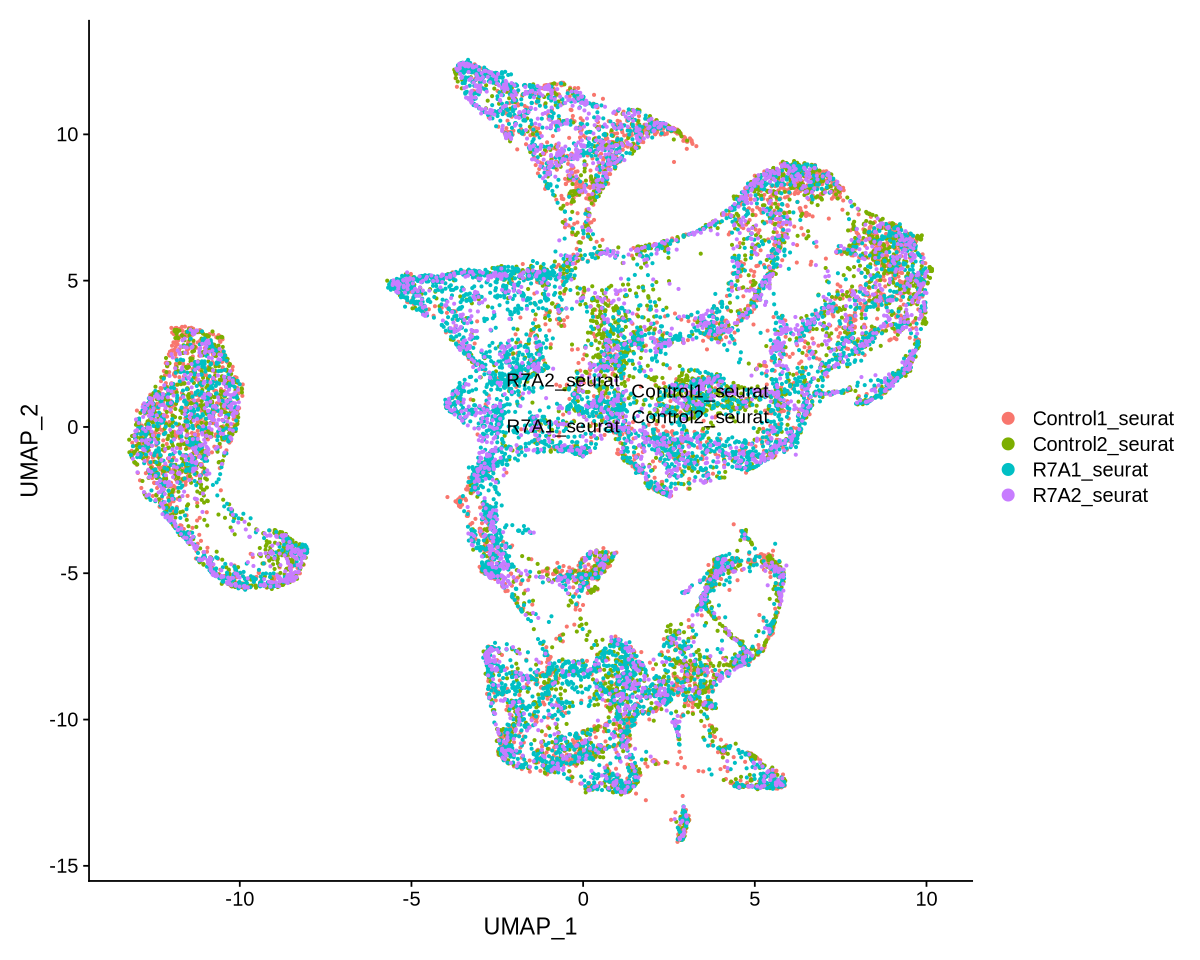
\includegraphics{tutorial-2024_files/figure-pdf/fig-umapint-output-1.png}

}

\caption{\label{fig-umapint}UMAP of the integrated datasets.}

\end{figure}%

We save our integrated data

\begin{Shaded}
\begin{Highlighting}[]
\FunctionTok{SaveH5Seurat}\NormalTok{(}\AttributeTok{object =}\NormalTok{ seurat.integrated, }\AttributeTok{filename =} \StringTok{"seurat.integrated.h5Seurat"}\NormalTok{, }\AttributeTok{overwrite=}\ConstantTok{TRUE}\NormalTok{)}
\end{Highlighting}
\end{Shaded}

\begin{verbatim}
Warning message:
“Overwriting previous file seurat.integrated.h5Seurat”
Creating h5Seurat file for version 3.1.5.9900

Adding counts for SCT

Adding data for SCT

Adding scale.data for SCT

No variable features found for SCT

No feature-level metadata found for SCT

Writing out SCTModel.list for SCT

Adding counts for RNA

Adding data for RNA

No variable features found for RNA

No feature-level metadata found for RNA

Adding data for integrated

Adding scale.data for integrated

Adding variable features for integrated

No feature-level metadata found for integrated

Writing out SCTModel.list for integrated

Adding cell embeddings for pca

Adding loadings for pca

No projected loadings for pca

Adding standard deviations for pca

No JackStraw data for pca

Adding cell embeddings for umap

No loadings for umap

No projected loadings for umap

No standard deviations for umap

No JackStraw data for umap
\end{verbatim}

\subsection{Clustering and cell type
assignment}\label{clustering-and-cell-type-assignment}

We perform clustering on the data using the leiden algorithm
(blondel\_fast\_2008, Traag, Waltman, and Van Eck (2019)). Then, we look
at a typical strategy of \textbf{naming clusters by visualizing known
markers}. Since this is very subjective and biased, we then resort to
naming cell types \textbf{using a reference annotated dataset}. An
overview of cell type assignment procedures can be found at Cheng et al.
(2023).

\begin{Shaded}
\begin{Highlighting}[]
\NormalTok{seurat.integrated }\OtherTok{\textless{}{-}}  \FunctionTok{LoadH5Seurat}\NormalTok{(}\StringTok{"seurat.integrated.h5Seurat"}\NormalTok{, }\AttributeTok{verbose=}\ConstantTok{FALSE}\NormalTok{)}
\end{Highlighting}
\end{Shaded}

\begin{verbatim}
Validating h5Seurat file

Warning message:
“Adding a command log without an assay associated with it”
\end{verbatim}

Clustering function \texttt{FindClusters}. The resolution is used to
change the number of clusters. We do not need many, so we set on to
0.25. Usual values range between 0.1 and 1.

\begin{Shaded}
\begin{Highlighting}[]
\NormalTok{seurat.integrated }\OtherTok{\textless{}{-}} \FunctionTok{FindClusters}\NormalTok{(}\AttributeTok{object =}\NormalTok{ seurat.integrated, }\AttributeTok{resolution =}\NormalTok{ .}\DecValTok{25}\NormalTok{)}
\end{Highlighting}
\end{Shaded}

\begin{verbatim}
Modularity Optimizer version 1.3.0 by Ludo Waltman and Nees Jan van Eck

Number of nodes: 17721
Number of edges: 165857

Running Louvain algorithm...
Maximum modularity in 10 random starts: 0.9631
Number of communities: 21
Elapsed time: 0 seconds
\end{verbatim}

\begin{verbatim}
Warning message:
“UNRELIABLE VALUE: One of the ‘future.apply’ iterations (‘future_lapply-1’) unexpectedly generated random numbers without declaring so. There is a risk that those random numbers are not statistically sound and the overall results might be invalid. To fix this, specify 'future.seed=TRUE'. This ensures that proper, parallel-safe random numbers are produced via the L'Ecuyer-CMRG method. To disable this check, use 'future.seed = NULL', or set option 'future.rng.onMisuse' to "ignore".”
\end{verbatim}

The clusters are saved in the meta data table as
\texttt{integrated\_snn\_res.0.25}. \textbf{Note that the name changes
with the resolution}. Also observe how much metadata we have: many
columns come from tools we have applied, such as doubletfinder (DF) and
nearest neighbor distances (snn).

\begin{Shaded}
\begin{Highlighting}[]
\FunctionTok{head}\NormalTok{( seurat.integrated}\SpecialCharTok{@}\NormalTok{meta.data )}
\end{Highlighting}
\end{Shaded}

A data.frame: 6 × 18

\begin{longtable}[]{@{}
  >{\raggedright\arraybackslash}p{(\columnwidth - 36\tabcolsep) * \real{0.0526}}
  >{\raggedright\arraybackslash}p{(\columnwidth - 36\tabcolsep) * \real{0.0526}}
  >{\raggedright\arraybackslash}p{(\columnwidth - 36\tabcolsep) * \real{0.0526}}
  >{\raggedright\arraybackslash}p{(\columnwidth - 36\tabcolsep) * \real{0.0526}}
  >{\raggedright\arraybackslash}p{(\columnwidth - 36\tabcolsep) * \real{0.0526}}
  >{\raggedright\arraybackslash}p{(\columnwidth - 36\tabcolsep) * \real{0.0526}}
  >{\raggedright\arraybackslash}p{(\columnwidth - 36\tabcolsep) * \real{0.0526}}
  >{\raggedright\arraybackslash}p{(\columnwidth - 36\tabcolsep) * \real{0.0526}}
  >{\raggedright\arraybackslash}p{(\columnwidth - 36\tabcolsep) * \real{0.0526}}
  >{\raggedright\arraybackslash}p{(\columnwidth - 36\tabcolsep) * \real{0.0526}}
  >{\raggedright\arraybackslash}p{(\columnwidth - 36\tabcolsep) * \real{0.0526}}
  >{\raggedright\arraybackslash}p{(\columnwidth - 36\tabcolsep) * \real{0.0526}}
  >{\raggedright\arraybackslash}p{(\columnwidth - 36\tabcolsep) * \real{0.0526}}
  >{\raggedright\arraybackslash}p{(\columnwidth - 36\tabcolsep) * \real{0.0526}}
  >{\raggedright\arraybackslash}p{(\columnwidth - 36\tabcolsep) * \real{0.0526}}
  >{\raggedright\arraybackslash}p{(\columnwidth - 36\tabcolsep) * \real{0.0526}}
  >{\raggedright\arraybackslash}p{(\columnwidth - 36\tabcolsep) * \real{0.0526}}
  >{\raggedright\arraybackslash}p{(\columnwidth - 36\tabcolsep) * \real{0.0526}}
  >{\raggedright\arraybackslash}p{(\columnwidth - 36\tabcolsep) * \real{0.0526}}@{}}
\toprule\noalign{}
\begin{minipage}[b]{\linewidth}\raggedright
\end{minipage} & \begin{minipage}[b]{\linewidth}\raggedright
nCount\_RNA \textless dbl\textgreater{}
\end{minipage} & \begin{minipage}[b]{\linewidth}\raggedright
nFeature\_RNA \textless int\textgreater{}
\end{minipage} & \begin{minipage}[b]{\linewidth}\raggedright
nCount\_SCT \textless dbl\textgreater{}
\end{minipage} & \begin{minipage}[b]{\linewidth}\raggedright
nFeature\_SCT \textless int\textgreater{}
\end{minipage} & \begin{minipage}[b]{\linewidth}\raggedright
orig.ident \textless chr\textgreater{}
\end{minipage} & \begin{minipage}[b]{\linewidth}\raggedright
Condition \textless chr\textgreater{}
\end{minipage} & \begin{minipage}[b]{\linewidth}\raggedright
percent.mt \textless dbl\textgreater{}
\end{minipage} & \begin{minipage}[b]{\linewidth}\raggedright
percent.chloroplast \textless dbl\textgreater{}
\end{minipage} & \begin{minipage}[b]{\linewidth}\raggedright
pANN\_0.25\_0.09\_609 \textless dbl\textgreater{}
\end{minipage} & \begin{minipage}[b]{\linewidth}\raggedright
DF.classifications\_0.25\_0.09\_609 \textless chr\textgreater{}
\end{minipage} & \begin{minipage}[b]{\linewidth}\raggedright
pANN\_0.25\_0.09\_329 \textless dbl\textgreater{}
\end{minipage} & \begin{minipage}[b]{\linewidth}\raggedright
DF.classifications\_0.25\_0.09\_329 \textless chr\textgreater{}
\end{minipage} & \begin{minipage}[b]{\linewidth}\raggedright
pANN\_0.25\_0.09\_309 \textless dbl\textgreater{}
\end{minipage} & \begin{minipage}[b]{\linewidth}\raggedright
DF.classifications\_0.25\_0.09\_309 \textless chr\textgreater{}
\end{minipage} & \begin{minipage}[b]{\linewidth}\raggedright
pANN\_0.25\_0.09\_110 \textless dbl\textgreater{}
\end{minipage} & \begin{minipage}[b]{\linewidth}\raggedright
DF.classifications\_0.25\_0.09\_110 \textless chr\textgreater{}
\end{minipage} & \begin{minipage}[b]{\linewidth}\raggedright
integrated\_snn\_res.0.25 \textless fct\textgreater{}
\end{minipage} & \begin{minipage}[b]{\linewidth}\raggedright
seurat\_clusters \textless fct\textgreater{}
\end{minipage} \\
\midrule\noalign{}
\endhead
\bottomrule\noalign{}
\endlastfoot
AAACCCACATGATCTG-1\_1 & 20942 & 4711 & 11291 & 4192 & Control1\_seurat &
Control & 0.4775093 & 0.12415242 & 0.2299688 & Singlet & NA & NA & NA &
NA & NA & NA & 4 & 4 \\
AAACCCAGTAGCTTGT-1\_1 & 29105 & 5157 & 10486 & 3382 & Control1\_seurat &
Control & 0.2954819 & 0.05497337 & 0.2695109 & Singlet & NA & NA & NA &
NA & NA & NA & 9 & 9 \\
AAACCCAGTCTCTCAC-1\_1 & 6115 & 2124 & 10086 & 2163 & Control1\_seurat &
Control & 1.6026165 & 0.01635323 & 0.1904266 & Singlet & NA & NA & NA &
NA & NA & NA & 0 & 0 \\
AAACCCATCACCTTGC-1\_1 & 7410 & 2988 & 10003 & 2985 & Control1\_seurat &
Control & 0.5263158 & 0.09446694 & 0.2466181 & Singlet & NA & NA & NA &
NA & NA & NA & 16 & 16 \\
AAACGAAAGTCCTGTA-1\_1 & 5616 & 2034 & 9866 & 2097 & Control1\_seurat &
Control & 0.7122507 & 0.10683761 & 0.2382934 & Singlet & NA & NA & NA &
NA & NA & NA & 17 & 17 \\
AAACGAAAGTGTGTTC-1\_1 & 12580 & 3329 & 11180 & 3328 & Control1\_seurat &
Control & 0.1510334 & 0.06359300 & 0.2559834 & Singlet & NA & NA & NA &
NA & NA & NA & 2 & 2 \\
\end{longtable}

We can plot the clusters in the UMAP plot

\begin{Shaded}
\begin{Highlighting}[]
\FunctionTok{options}\NormalTok{(}\AttributeTok{repr.plot.width=}\DecValTok{10}\NormalTok{, }\AttributeTok{repr.plot.height=}\DecValTok{8}\NormalTok{)}
\FunctionTok{DimPlot}\NormalTok{(}\AttributeTok{object =}\NormalTok{ seurat.integrated, }\AttributeTok{reduction =} \StringTok{"umap"}\NormalTok{,  }\AttributeTok{label =}\NormalTok{ T, }\AttributeTok{repel =} \ConstantTok{TRUE}\NormalTok{, }\AttributeTok{pt.size =} \FloatTok{0.5}\NormalTok{)}
\end{Highlighting}
\end{Shaded}

\begin{figure}[H]

\centering{

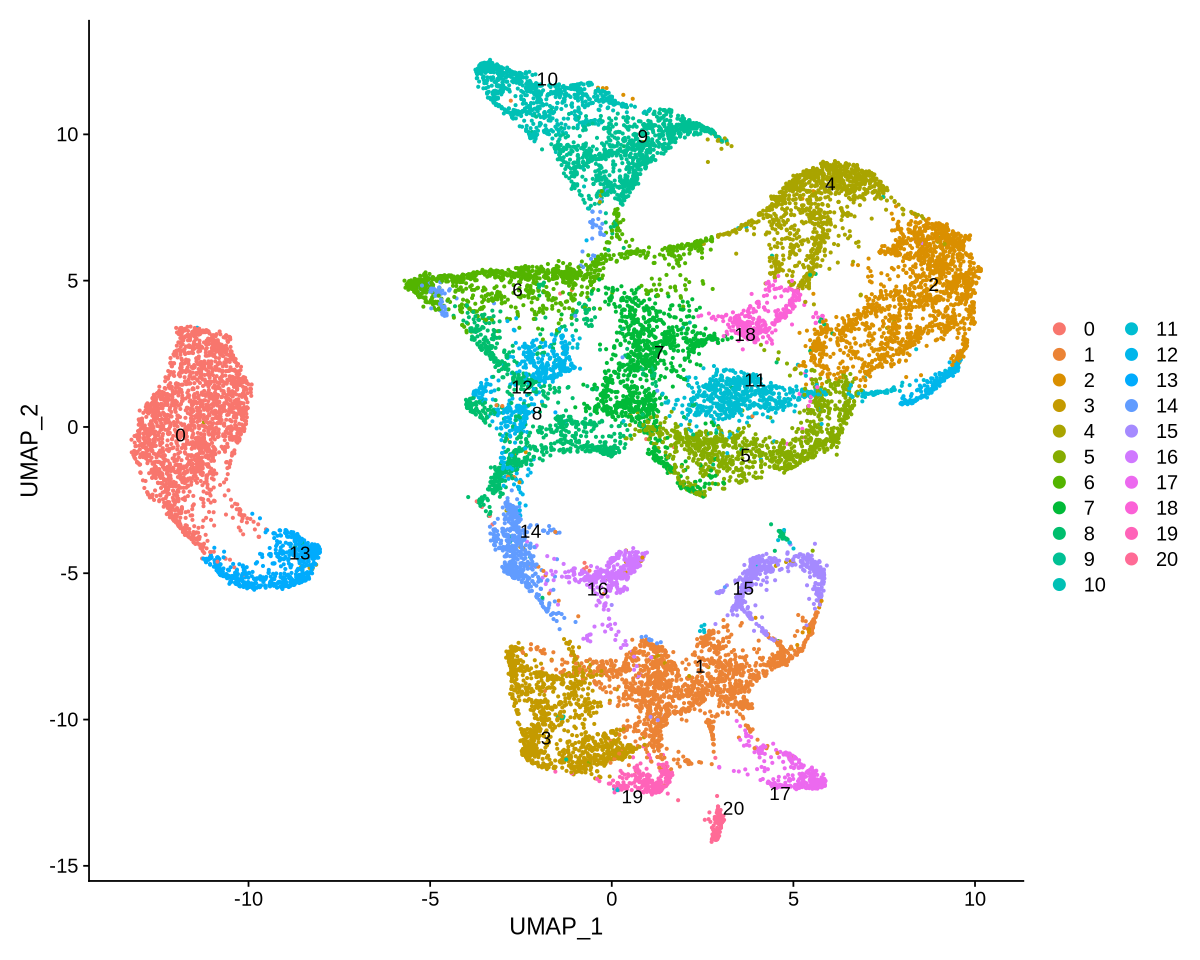
\includegraphics{tutorial-2024_files/figure-pdf/fig-umapleiden-output-1.png}

}

\caption{\label{fig-umapleiden}UMAP of the integrated datasets with
clusters (still unassigned to cell types).}

\end{figure}%

\subsubsection{Cluster assignment from visualized marker
scores}\label{cluster-assignment-from-visualized-marker-scores}

Here, we look at how to assign names based on known markers. In this
procedure, biological knowledge of the cell types is needed. Below,
there is a list of known markers for each cell type, extracted from the
supplementary data of Frank et al. (2023).

\begin{Shaded}
\begin{Highlighting}[]
\NormalTok{features\_list }\OtherTok{\textless{}{-}} \FunctionTok{list}\NormalTok{(}
    \StringTok{\textquotesingle{}Cortex\_scoring\textquotesingle{}} \OtherTok{=} \FunctionTok{c}\NormalTok{(}\StringTok{"LotjaGi1g1v0006200"}\NormalTok{,}
                 \StringTok{"LotjaGi1g1v0022100"}\NormalTok{,}
                 \StringTok{"LotjaGi1g1v0261700"}\NormalTok{,}
                 \StringTok{"LotjaGi1g1v0348000"}\NormalTok{,}
                 \StringTok{"LotjaGi2g1v0303000"}\NormalTok{,}
                 \StringTok{"LotjaGi3g1v0505900"}\NormalTok{),}
    \StringTok{\textquotesingle{}Epidermis\_scoring\textquotesingle{}} \OtherTok{=} \FunctionTok{c}\NormalTok{(}\StringTok{"LotjaGi1g1v0080000"}\NormalTok{,}
                    \StringTok{"LotjaGi1g1v0377600"}\NormalTok{,}
                    \StringTok{"LotjaGi1g1v0613100"}\NormalTok{,}
                    \StringTok{"LotjaGi3g1v0070500"}\NormalTok{),}
    \StringTok{\textquotesingle{}Endodermis\_scoring\textquotesingle{}} \OtherTok{=} \FunctionTok{c}\NormalTok{(}\StringTok{"LotjaGi1g1v0114400"}\NormalTok{,}
                     \StringTok{"LotjaGi1g1v0221300"}\NormalTok{,}
                     \StringTok{"LotjaGi1g1v0240900{-}LC"}\NormalTok{,}
                     \StringTok{"LotjaGi1g1v0707500"}\NormalTok{), }
    \StringTok{\textquotesingle{}RootCap\_scoring\textquotesingle{}} \OtherTok{=} \FunctionTok{c}\NormalTok{(}\StringTok{"LotjaGi1g1v0020900"}\NormalTok{,}
                   \StringTok{"LotjaGi1g1v0039700{-}LC"}\NormalTok{,}
                   \StringTok{"LotjaGi1g1v0040300"}\NormalTok{,}
                   \StringTok{"LotjaGi1g1v0147500"}\NormalTok{),  }
    \StringTok{\textquotesingle{}Meristem\_scoring\textquotesingle{}}\OtherTok{=} \FunctionTok{c}\NormalTok{(}\StringTok{"LotjaGi4g1v0300900"}\NormalTok{,}
                         \StringTok{"LotjaGi6g1v0056500"}\NormalTok{,}
                         \StringTok{"LotjaGi1g1v0594200"}\NormalTok{),}
    \StringTok{\textquotesingle{}Phloem\_scoring\textquotesingle{}}\OtherTok{=} \FunctionTok{c}\NormalTok{(}\StringTok{"LotjaGi1g1v0028800"}\NormalTok{,}
                \StringTok{"LotjaGi1g1v0085900"}\NormalTok{,}
                \StringTok{"LotjaGi1g1v0119300"}\NormalTok{,}
                \StringTok{"LotjaGi1g1v0149100"}\NormalTok{),}
    \StringTok{\textquotesingle{}QuiescentCenter\_scoring\textquotesingle{}} \OtherTok{=} \FunctionTok{c}\NormalTok{(}\StringTok{"LotjaGi1g1v0004300"}\NormalTok{,}
                           \StringTok{"LotjaGi1g1v0021400"}\NormalTok{,}
                           \StringTok{"LotjaGi1g1v0052700"}\NormalTok{,}
                           \StringTok{"LotjaGi1g1v0084000"}\NormalTok{),}
    \StringTok{\textquotesingle{}RootHair\_scoring\textquotesingle{}}\OtherTok{=} \FunctionTok{c}\NormalTok{(}\StringTok{"LotjaGi1g1v0014300"}\NormalTok{,}
                   \StringTok{"LotjaGi1g1v0109000"}\NormalTok{,}
                   \StringTok{"LotjaGi1g1v0109100"}\NormalTok{,}
                   \StringTok{"LLotjaGi1g1v0143900"}\NormalTok{),  }
    \StringTok{\textquotesingle{}Pericycle\_scoring\textquotesingle{}}\OtherTok{=} \FunctionTok{c}\NormalTok{(}\StringTok{"LotjaGi3g1v0222100"}\NormalTok{,}
                   \StringTok{"LotjaGi3g1v0395900{-}LC"}\NormalTok{,}
                   \StringTok{"LotjaGi5g1v0166000{-}LC"}\NormalTok{,}
                   \StringTok{"LotjaGi3g1v0395500{-}LC"}\NormalTok{,}
                   \StringTok{"LotjaGi1g1v0783700{-}LC"}\NormalTok{,}
                   \StringTok{"LotjaGi2g1v0333200"}\NormalTok{,}
                   \StringTok{"LotjaGi4g1v0293000{-}LC"}\NormalTok{),     }
    \StringTok{\textquotesingle{}Stele\_scoring\textquotesingle{}} \OtherTok{=} \FunctionTok{c}\NormalTok{(}\StringTok{"LotjaGi2g1v0126700"}\NormalTok{,}
                \StringTok{"LotjaGi1g1v0558200"}\NormalTok{,}
                \StringTok{"LotjaGi4g1v0215500"}\NormalTok{,}
                \StringTok{"LotjaGi3g1v0174100"}\NormalTok{,}
                \StringTok{"LotjaGi5g1v0288600"}\NormalTok{,}
                \StringTok{"LotjaGi3g1v0129700"}\NormalTok{),}
    \StringTok{\textquotesingle{}Xylem\_scoring\textquotesingle{}} \OtherTok{=} \FunctionTok{c}\NormalTok{(}\StringTok{"LotjaGi1g1v0623100"}\NormalTok{,}
                \StringTok{"LotjaGi1g1v0569300"}\NormalTok{,}
                \StringTok{"LotjaGi1g1v0443000"}\NormalTok{,}
                \StringTok{"LotjaGi1g1v0428800"}\NormalTok{)}
\NormalTok{    )}
\end{Highlighting}
\end{Shaded}

Here, we need a function calculating the scores for each cell type. This
is the average expression of the markers in the list, from which we
remove the average expression of some control genes, which are supposed
not to be specific for the cell type of interest. The cells matching the
desired type should retain a high score.

\begin{Shaded}
\begin{Highlighting}[]
\NormalTok{seurat.clustered }\OtherTok{\textless{}{-}} \FunctionTok{AddModuleScore}\NormalTok{(}
  \AttributeTok{object =}\NormalTok{ seurat.integrated,}
  \AttributeTok{features =}\NormalTok{ features\_list,}
  \AttributeTok{ctrl =} \DecValTok{5}\NormalTok{,}
  \AttributeTok{name =} \StringTok{\textquotesingle{}LJ\_scores\textquotesingle{}}
\NormalTok{)}
\end{Highlighting}
\end{Shaded}

\begin{verbatim}
Warning message:
“The following features are not present in the object: LLotjaGi1g1v0143900, not searching for symbol synonyms”
\end{verbatim}

We also apply a function (from \texttt{script.R}) to rename the scores
in the metadata. Their names are not intuitive by default, they are all
called with the name chosen above and a number after it:

\begin{Shaded}
\begin{Highlighting}[]
\FunctionTok{names}\NormalTok{(seurat.clustered}\SpecialCharTok{@}\NormalTok{meta.data)}
\end{Highlighting}
\end{Shaded}

\begin{enumerate}
\def\labelenumi{\arabic{enumi}.}
\tightlist
\item
  `nCount\_RNA'
\item
  `nFeature\_RNA'
\item
  `nCount\_SCT'
\item
  `nFeature\_SCT'
\item
  `orig.ident'
\item
  `Condition'
\item
  `percent.mt'
\item
  `percent.chloroplast'
\item
  `pANN\_0.25\_0.09\_609'
\item
  `DF.classifications\_0.25\_0.09\_609'
\item
  `pANN\_0.25\_0.09\_329'
\item
  `DF.classifications\_0.25\_0.09\_329'
\item
  `pANN\_0.25\_0.09\_309'
\item
  `DF.classifications\_0.25\_0.09\_309'
\item
  `pANN\_0.25\_0.09\_110'
\item
  `DF.classifications\_0.25\_0.09\_110'
\item
  `integrated\_snn\_res.0.25'
\item
  `seurat\_clusters'
\item
  `LJ\_scores1'
\item
  `LJ\_scores2'
\item
  `LJ\_scores3'
\item
  `LJ\_scores4'
\item
  `LJ\_scores5'
\item
  `LJ\_scores6'
\item
  `LJ\_scores7'
\item
  `LJ\_scores8'
\item
  `LJ\_scores9'
\item
  `LJ\_scores10'
\item
  `LJ\_scores11'
\end{enumerate}

\begin{Shaded}
\begin{Highlighting}[]
\NormalTok{seurat.clustered }\OtherTok{\textless{}{-}} \FunctionTok{renameScores}\NormalTok{(}\AttributeTok{markers\_list =}\NormalTok{ features\_list, }\AttributeTok{seurat\_data =}\NormalTok{ seurat.clustered)      }
\end{Highlighting}
\end{Shaded}

\begin{verbatim}
Scores renamed FROM




TO



\end{verbatim}

\begin{verbatim}
LJ_scores1
LJ_scores2
LJ_scores3
LJ_scores4
LJ_scores5
LJ_scores6
LJ_scores7
LJ_scores8
LJ_scores9
LJ_scores10
LJ_scores11
Cortex_scoring
Epidermis_scoring
Endodermis_scoring
RootCap_scoring
Meristem_scoring
Phloem_scoring
QuiescentCenter_scoring
RootHair_scoring
Pericycle_scoring
Stele_scoring
Xylem_scoring
\end{verbatim}

Now we run the function \texttt{plotScoresUMAP} (from the file
\texttt{script.R}). In Figure~\ref{fig-scores} we can see that some
clusters are easy to classify (phloem and xylem), but many others are
not. This is mainly due to the fact that the change of many cell types
is a continuum, and this manual annotation is very subjective.

\begin{Shaded}
\begin{Highlighting}[]
\FunctionTok{plotScoresUMAP}\NormalTok{(}\AttributeTok{markers\_list =}\NormalTok{ features\_list, }\AttributeTok{seurat\_data =}\NormalTok{ seurat.clustered)                                  }
\end{Highlighting}
\end{Shaded}

\begin{figure}[H]

\centering{

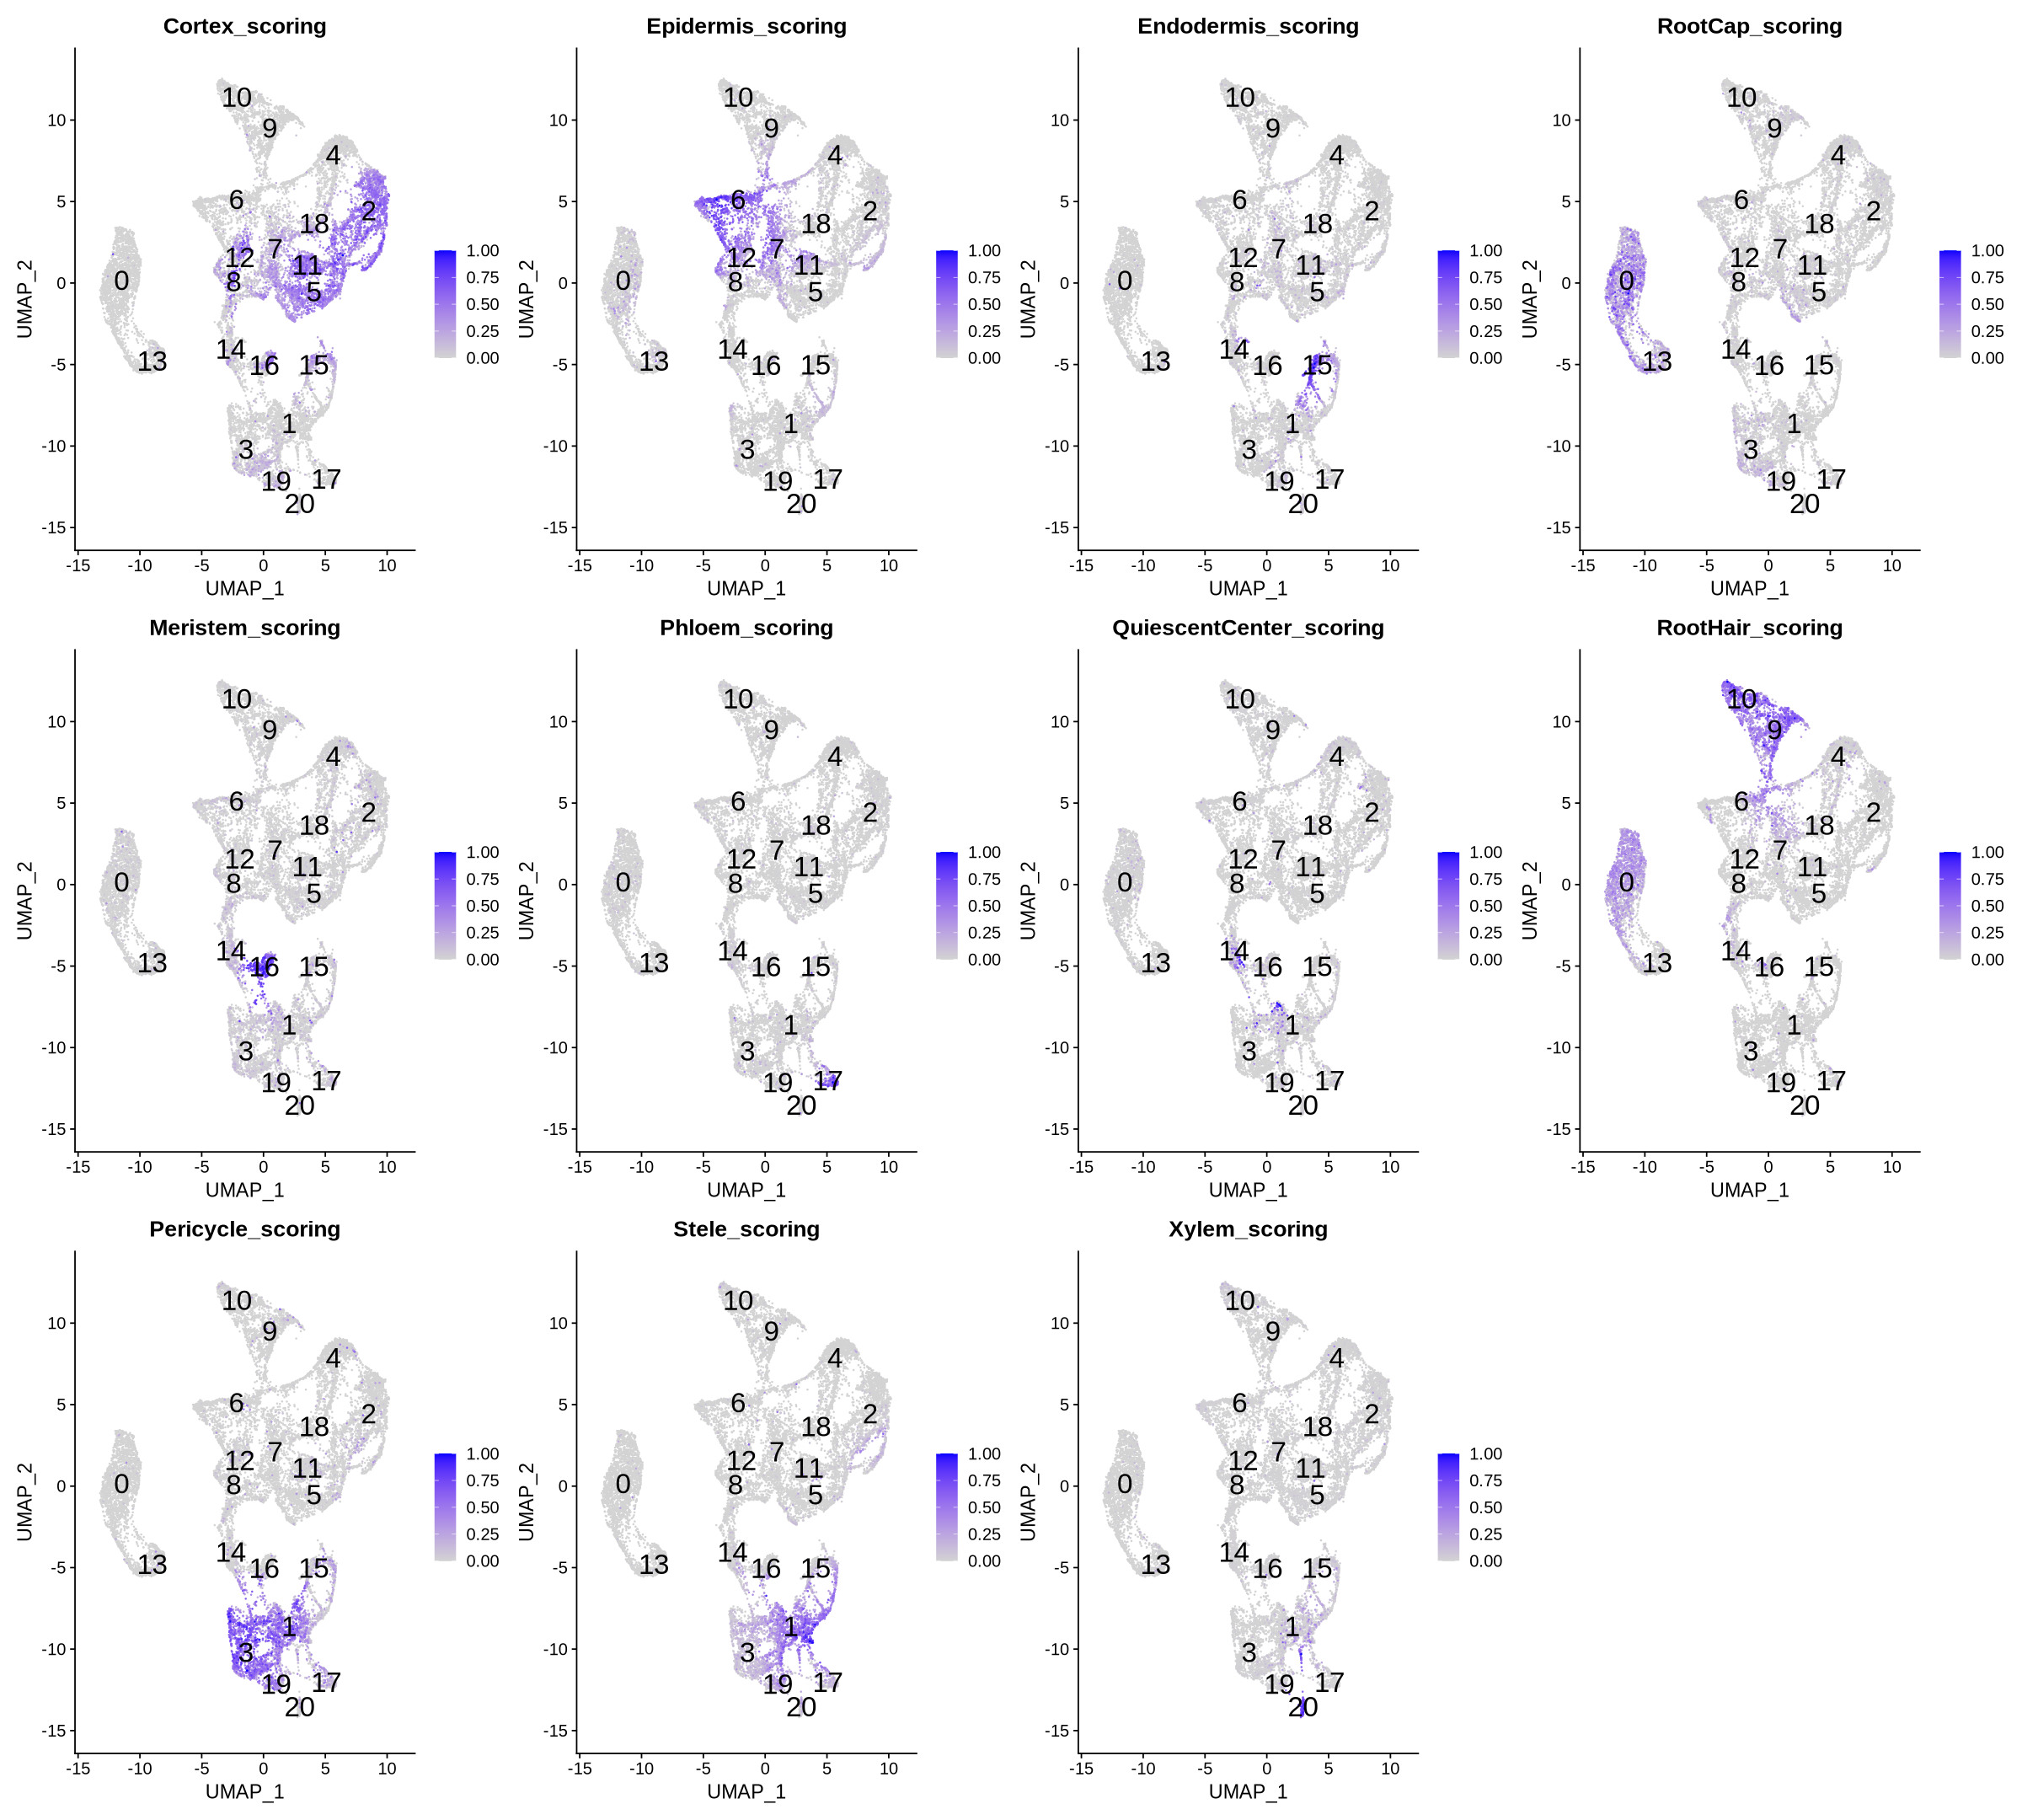
\includegraphics{tutorial-2024_files/figure-pdf/fig-scores-output-1.png}

}

\caption{\label{fig-scores}Scores of the list of markers for the Lotus
Japonicus clusters. Those should help identifying cell types by plotting
the average of markers subtracted the average of other random genes in
the data.}

\end{figure}%

Just for the sake of the exercise, we set some names to the clusters
below, at least for those ones that are well identifiable. Note that we
use \texttt{idents} to define which is the clustering to be considered
in use in the data.

\begin{Shaded}
\begin{Highlighting}[]
\FunctionTok{Idents}\NormalTok{(seurat.clustered) }\OtherTok{\textless{}{-}} \StringTok{\textquotesingle{}integrated\_snn\_res.0.25\textquotesingle{}}

\NormalTok{seurat.clustered }\OtherTok{\textless{}{-}} \FunctionTok{RenameIdents}\NormalTok{(}\AttributeTok{object =}\NormalTok{ seurat.clustered,}
                               \StringTok{"2"}\OtherTok{=}\StringTok{"Cortex"}\NormalTok{, }\StringTok{"5"}\OtherTok{=}\StringTok{"Cortex"}\NormalTok{, }\StringTok{"11"}\OtherTok{=}\StringTok{"Cortex"}\NormalTok{,}
                               \StringTok{"6"}\OtherTok{=}\StringTok{"Epidermis"}\NormalTok{, }\StringTok{"12"}\OtherTok{=}\StringTok{"Epidermis"}\NormalTok{, }\StringTok{"7"}\OtherTok{=}\StringTok{"Epidermis"}\NormalTok{,}
                               \StringTok{"15"}\OtherTok{=}\StringTok{"Endodermis"}\NormalTok{,  }
                               \StringTok{"0"}\OtherTok{=}\StringTok{"Root\_Cap"}\NormalTok{, }\StringTok{"13"}\OtherTok{=}\StringTok{"Root\_Cap"}\NormalTok{,}
                               \StringTok{"16"}\OtherTok{=}\StringTok{"Meristem"}\NormalTok{,  }
                               \StringTok{"17"}\OtherTok{=}\StringTok{"Phloem"}\NormalTok{,}
                               \StringTok{"10"}\OtherTok{=}\StringTok{"Root\_Hair"}\NormalTok{, }\StringTok{"9"}\OtherTok{=}\StringTok{"Root\_Hair"}\NormalTok{,}
                               \StringTok{"1"}\OtherTok{=}\StringTok{"PericycleStele"}\NormalTok{, }
                               \StringTok{"3"}\OtherTok{=}\StringTok{"Pericycle"}\NormalTok{, }\StringTok{"19"}\OtherTok{=}\StringTok{"Pericycle"}\NormalTok{,}
                               \StringTok{"20"}\OtherTok{=}\StringTok{"Xylem"}\NormalTok{)}
\end{Highlighting}
\end{Shaded}

we saved the renamed clusters in the metadata under \texttt{Cell\_types}

\begin{Shaded}
\begin{Highlighting}[]
\NormalTok{seurat.clustered}\SpecialCharTok{@}\NormalTok{meta.data}\SpecialCharTok{$}\NormalTok{Cell\_types }\OtherTok{\textless{}{-}} \FunctionTok{Idents}\NormalTok{(seurat.clustered)}
\end{Highlighting}
\end{Shaded}

It seems from Figure~\ref{fig-umapbyeye} that we named most clusters.
For some others we could not really be sure of the markers, and we will
use the reference-based assignment.

\begin{Shaded}
\begin{Highlighting}[]
\FunctionTok{options}\NormalTok{(}\AttributeTok{repr.plot.width=}\DecValTok{10}\NormalTok{, }\AttributeTok{repr.plot.height=}\DecValTok{10}\NormalTok{)}
\FunctionTok{DimPlot}\NormalTok{(}\AttributeTok{object =}\NormalTok{ seurat.clustered, }\AttributeTok{reduction =} \StringTok{"umap"}\NormalTok{, }\AttributeTok{repel =} \ConstantTok{TRUE}\NormalTok{, }\AttributeTok{label=}\NormalTok{T, }\AttributeTok{pt.size =} \DecValTok{2}\NormalTok{, }\AttributeTok{label.size =} \DecValTok{5}\NormalTok{)}
\end{Highlighting}
\end{Shaded}

\begin{figure}[H]

\centering{

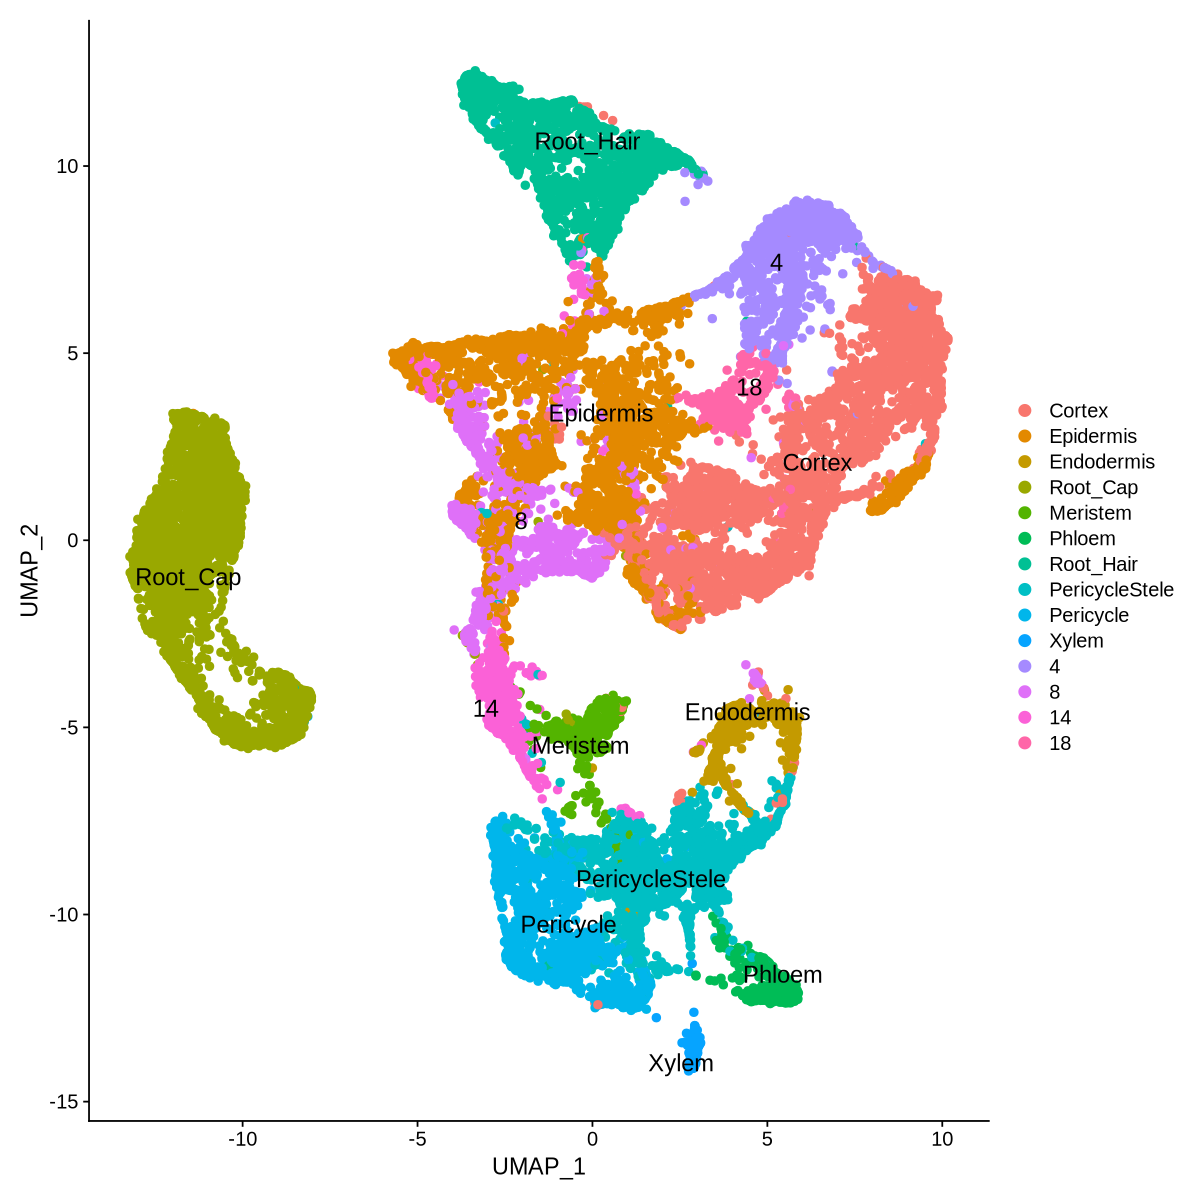
\includegraphics{tutorial-2024_files/figure-pdf/fig-umapbyeye-output-1.png}

}

\caption{\label{fig-umapbyeye}UMAP of the integrated datasets with
clusters assigned by looking at markers scores. Note how we could not
determine clearly some of the clusters, because of few cells with high
scores (cluster 11, which might be epidermis; and cluster 16, which
might be quiescent center) or cells that might be a mix of two types
(like Pericycle and Stele).}

\end{figure}%

\paragraph{Optional: assigning a mixed
cluster}\label{optional-assigning-a-mixed-cluster}

The cluster \texttt{Pericycle\_Stele} is probably a mix of the Pericycle
and Stele, because it shows markers from both. We can assign at each
cell of the cluster one of the cell types based on which marker score is
highest. First we save the old clustering in the metadata to avoid
losing it

\begin{Shaded}
\begin{Highlighting}[]
\NormalTok{seurat.clustered}\SpecialCharTok{@}\NormalTok{meta.data}\SpecialCharTok{$}\NormalTok{Cell\_types\_old }\OtherTok{\textless{}{-}} \FunctionTok{Idents}\NormalTok{(seurat.clustered)}
\end{Highlighting}
\end{Shaded}

and then reassign the name to the cluster \texttt{Pericycle\_Stele}
checking the markers score of each cell.

\begin{Shaded}
\begin{Highlighting}[]
\NormalTok{peri }\OtherTok{\textless{}{-}}\NormalTok{ seurat.clustered}\SpecialCharTok{@}\NormalTok{meta.data}\SpecialCharTok{$}\NormalTok{Pericycle\_scoring[seurat.clustered}\SpecialCharTok{@}\NormalTok{meta.data}\SpecialCharTok{$}\NormalTok{Cell\_types }\SpecialCharTok{==} \StringTok{\textquotesingle{}PericycleStele\textquotesingle{}}\NormalTok{]}
\NormalTok{stel }\OtherTok{\textless{}{-}}\NormalTok{ seurat.clustered}\SpecialCharTok{@}\NormalTok{meta.data}\SpecialCharTok{$}\NormalTok{Stele\_scoring[seurat.clustered}\SpecialCharTok{@}\NormalTok{meta.data}\SpecialCharTok{$}\NormalTok{Cell\_types }\SpecialCharTok{==} \StringTok{\textquotesingle{}PericycleStele\textquotesingle{}}\NormalTok{]}
\NormalTok{peri\_stele }\OtherTok{\textless{}{-}}\NormalTok{ peri}\SpecialCharTok{\textgreater{}=}\NormalTok{stel}
\NormalTok{finalcl }\OtherTok{=} \FunctionTok{c}\NormalTok{()}
\ControlFlowTok{for}\NormalTok{(i }\ControlFlowTok{in}\NormalTok{ peri\_stele)}
\NormalTok{    finalcl }\OtherTok{=} \FunctionTok{c}\NormalTok{(finalcl, }\FunctionTok{ifelse}\NormalTok{(i, }\StringTok{"Pericycle"}\NormalTok{, }\StringTok{"Stele"}\NormalTok{))}

\NormalTok{celltypes }\OtherTok{\textless{}{-}} \FunctionTok{unfactor}\NormalTok{(seurat.clustered}\SpecialCharTok{@}\NormalTok{meta.data}\SpecialCharTok{$}\NormalTok{Cell\_types)}
\NormalTok{celltypes[seurat.clustered}\SpecialCharTok{@}\NormalTok{meta.data}\SpecialCharTok{$}\NormalTok{Cell\_types }\SpecialCharTok{==} \StringTok{\textquotesingle{}PericycleStele\textquotesingle{}}\NormalTok{] }\OtherTok{\textless{}{-}}\NormalTok{ finalcl}
\NormalTok{seurat.clustered}\SpecialCharTok{@}\NormalTok{meta.data}\SpecialCharTok{$}\NormalTok{Cell\_types }\OtherTok{\textless{}{-}}\NormalTok{ celltypes}
\FunctionTok{Idents}\NormalTok{(seurat.clustered) }\OtherTok{\textless{}{-}}\NormalTok{ seurat.clustered}\SpecialCharTok{@}\NormalTok{meta.data}\SpecialCharTok{$}\NormalTok{Cell\_types}
\end{Highlighting}
\end{Shaded}

We managed to get a meaningful separation between the two clusters!

\begin{Shaded}
\begin{Highlighting}[]
\FunctionTok{options}\NormalTok{(}\AttributeTok{repr.plot.width=}\DecValTok{10}\NormalTok{, }\AttributeTok{repr.plot.height=}\DecValTok{10}\NormalTok{)}
\FunctionTok{DimPlot}\NormalTok{(}\AttributeTok{object =}\NormalTok{ seurat.clustered, }\AttributeTok{reduction =} \StringTok{"umap"}\NormalTok{, }\AttributeTok{repel =} \ConstantTok{TRUE}\NormalTok{, }\AttributeTok{label=}\NormalTok{T, }\AttributeTok{pt.size =} \DecValTok{2}\NormalTok{, }\AttributeTok{label.size =} \DecValTok{5}\NormalTok{)}
\end{Highlighting}
\end{Shaded}

\begin{figure}[H]

\centering{

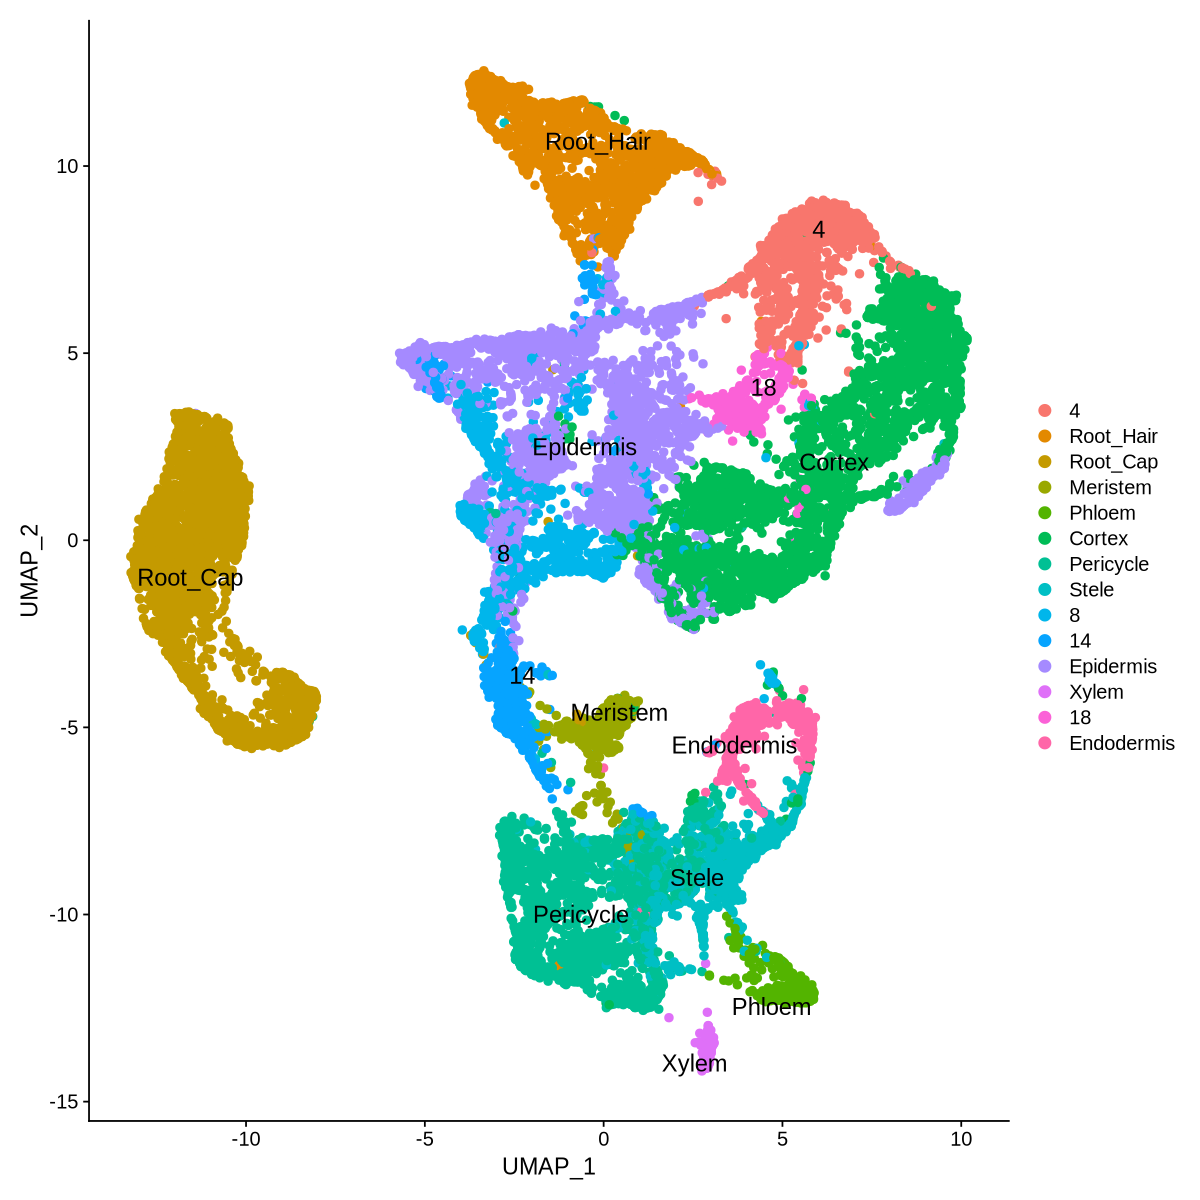
\includegraphics{tutorial-2024_files/figure-pdf/fig-umapsubcluster-output-1.png}

}

\caption{\label{fig-umapsubcluster}UMAP of the integrated datasets with
clusters assigned by looking at markers scores and separated clusters of
Peicycle and Stele. In this case, the subclustering has clearly been a
success.}

\end{figure}%

\subsubsection{Cluster assignment from an annotated
dataset}\label{cluster-assignment-from-an-annotated-dataset}

We now use the annotated data from Frank et al. (2023) (which is the
same we are using in the tutorial) to transfer data labels to our own
processed data. More about label transfer can be read at Stuart et al.
(2019). We load the data from the paper and define reference and query
data.

\begin{Shaded}
\begin{Highlighting}[]
\NormalTok{seurat.reference }\OtherTok{\textless{}{-}} \FunctionTok{readRDS}\NormalTok{(}\StringTok{"data\_lavinia.RDS"}\NormalTok{)}
\end{Highlighting}
\end{Shaded}

\begin{Shaded}
\begin{Highlighting}[]
\NormalTok{seurat.query }\OtherTok{\textless{}{-}}\NormalTok{ seurat.clustered}
\end{Highlighting}
\end{Shaded}

We have to define the data integration between query and reference
before we can transfer the cluster names. For the algorithm to work, we
need to use the ``RNA'' assay, which contains raw expression values.

\begin{Shaded}
\begin{Highlighting}[]
\FunctionTok{DefaultAssay}\NormalTok{(seurat.query) }\OtherTok{\textless{}{-}} \StringTok{"RNA"}
\end{Highlighting}
\end{Shaded}

\begin{Shaded}
\begin{Highlighting}[]
\NormalTok{lotusjaponicus.anchors }\OtherTok{\textless{}{-}} \FunctionTok{FindTransferAnchors}\NormalTok{(}\AttributeTok{reference =}\NormalTok{ seurat.reference, }
                                        \AttributeTok{features =} \FunctionTok{intersect}\NormalTok{( }\FunctionTok{rownames}\NormalTok{(seurat.query), }
                                                   \FunctionTok{rownames}\NormalTok{( seurat.reference[[}\StringTok{\textquotesingle{}SCT\textquotesingle{}}\NormalTok{]]}\SpecialCharTok{@}\NormalTok{scale.data ) ),}
                                        \AttributeTok{query =}\NormalTok{ seurat.query, }\AttributeTok{dims =} \DecValTok{1}\SpecialCharTok{:}\DecValTok{20}\NormalTok{, }
                                        \AttributeTok{reference.reduction =} \StringTok{"pca"}\NormalTok{,}
                                        \AttributeTok{reference.assay=}\StringTok{\textquotesingle{}RNA\textquotesingle{}}\NormalTok{)}
\end{Highlighting}
\end{Shaded}

\begin{verbatim}
Projecting cell embeddings

Finding neighborhoods

Finding anchors

    Found 25859 anchors

Filtering anchors

    Retained 13194 anchors
\end{verbatim}

Calculating the integration of the labels from the reference takes time.
So we save the calculated anchors for the integration. If you need to
rerun the code, skip the command above and instead load the data with
\texttt{readRDS} below.

\begin{Shaded}
\begin{Highlighting}[]
\FunctionTok{saveRDS}\NormalTok{(lotusjaponicus.anchors, }\AttributeTok{file =} \StringTok{"anchors.RDS"}\NormalTok{)}
\end{Highlighting}
\end{Shaded}

\begin{Shaded}
\begin{Highlighting}[]
\NormalTok{lotusjaponicus.anchors }\OtherTok{\textless{}{-}} \FunctionTok{readRDS}\NormalTok{(}\StringTok{"anchors.RDS"}\NormalTok{)}
\end{Highlighting}
\end{Shaded}

Now it is finally time to transfer the labels and add them to the
metadata. The column in the metadata is called by default
\texttt{predicted.id}.

\begin{Shaded}
\begin{Highlighting}[]
\NormalTok{predictions }\OtherTok{\textless{}{-}} \FunctionTok{TransferData}\NormalTok{(}\AttributeTok{anchorset =}\NormalTok{ lotusjaponicus.anchors, }
                            \AttributeTok{refdata =} \FunctionTok{Idents}\NormalTok{(seurat.reference), }
                            \AttributeTok{dims =} \DecValTok{1}\SpecialCharTok{:}\DecValTok{20}\NormalTok{)}
\end{Highlighting}
\end{Shaded}

\begin{verbatim}
Finding integration vectors

Finding integration vector weights

Predicting cell labels
\end{verbatim}

\begin{Shaded}
\begin{Highlighting}[]
\NormalTok{seurat.clustered }\OtherTok{\textless{}{-}} \FunctionTok{AddMetaData}\NormalTok{(seurat.clustered, }\AttributeTok{metadata =}\NormalTok{ predictions[}\StringTok{\textquotesingle{}predicted.id\textquotesingle{}}\NormalTok{])}
\end{Highlighting}
\end{Shaded}

Just as a reminder of what is in the metadata, we can quickly look at
the column names. Those are ordered by when we added things along the
analysis. If you read the names, you can recognize part of the analysis
steps until now.

\begin{Shaded}
\begin{Highlighting}[]
\FunctionTok{names}\NormalTok{( seurat.clustered}\SpecialCharTok{@}\NormalTok{meta.data )}
\end{Highlighting}
\end{Shaded}

\begin{enumerate}
\def\labelenumi{\arabic{enumi}.}
\tightlist
\item
  `nCount\_RNA'
\item
  `nFeature\_RNA'
\item
  `nCount\_SCT'
\item
  `nFeature\_SCT'
\item
  `orig.ident'
\item
  `Condition'
\item
  `percent.mt'
\item
  `percent.chloroplast'
\item
  `pANN\_0.25\_0.09\_609'
\item
  `DF.classifications\_0.25\_0.09\_609'
\item
  `pANN\_0.25\_0.09\_329'
\item
  `DF.classifications\_0.25\_0.09\_329'
\item
  `pANN\_0.25\_0.09\_309'
\item
  `DF.classifications\_0.25\_0.09\_309'
\item
  `pANN\_0.25\_0.09\_110'
\item
  `DF.classifications\_0.25\_0.09\_110'
\item
  `integrated\_snn\_res.0.25'
\item
  `seurat\_clusters'
\item
  `Cortex\_scoring'
\item
  `Epidermis\_scoring'
\item
  `Endodermis\_scoring'
\item
  `RootCap\_scoring'
\item
  `Meristem\_scoring'
\item
  `Phloem\_scoring'
\item
  `QuiescentCenter\_scoring'
\item
  `RootHair\_scoring'
\item
  `Pericycle\_scoring'
\item
  `Stele\_scoring'
\item
  `Xylem\_scoring'
\item
  `Cell\_types'
\item
  `Cell\_types\_old'
\item
  `predicted.id'
\end{enumerate}

Here we define as clustering for the data and the plots, the one
transfered just before. We then have a look at Figure~\ref{fig-transfer}
to observe that the labels look fine.

\begin{Shaded}
\begin{Highlighting}[]
\FunctionTok{Idents}\NormalTok{(seurat.clustered) }\OtherTok{\textless{}{-}} \StringTok{\textquotesingle{}predicted.id\textquotesingle{}}
\end{Highlighting}
\end{Shaded}

\begin{figure}

\centering{

\captionsetup{labelsep=none}

\begin{Shaded}
\begin{Highlighting}[]
\FunctionTok{options}\NormalTok{(}\AttributeTok{repr.plot.width=}\DecValTok{10}\NormalTok{, }\AttributeTok{repr.plot.height=}\DecValTok{10}\NormalTok{)}
\FunctionTok{DimPlot}\NormalTok{(}\AttributeTok{object =}\NormalTok{ seurat.clustered, }
        \AttributeTok{reduction =} \StringTok{"umap"}\NormalTok{, }
        \AttributeTok{repel =} \ConstantTok{TRUE}\NormalTok{, }\AttributeTok{label=}\NormalTok{T, }
        \AttributeTok{pt.size =} \FloatTok{0.5}\NormalTok{, }\AttributeTok{label.size =} \DecValTok{10}\NormalTok{, )}
\end{Highlighting}
\end{Shaded}

\begin{verbatim}
ERROR: Error in DimPlot(object = seurat.clustered, reduction = "umap", repel = TRUE, : could not find function "DimPlot"
\end{verbatim}

}

\caption{\label{fig-transfer}}

\end{figure}%

We save the data

\begin{Shaded}
\begin{Highlighting}[]
\FunctionTok{SaveH5Seurat}\NormalTok{(}\AttributeTok{object =}\NormalTok{ seurat.clustered, }
             \AttributeTok{filename =} \StringTok{"seurat.clustered.h5Seurat"}\NormalTok{, }
             \AttributeTok{overwrite =} \ConstantTok{TRUE}\NormalTok{,}
             \AttributeTok{verbose=}\ConstantTok{FALSE}\NormalTok{)}
\end{Highlighting}
\end{Shaded}

\begin{verbatim}
Warning message:
“Overwriting previous file seurat.clustered.h5Seurat”
Creating h5Seurat file for version 3.1.5.9900
\end{verbatim}

\section{Gene Expression Analysis}\label{sec-geneanalysis}

In this section we explore the gene expression through

\begin{itemize}
\tightlist
\item
  inferring \textbf{conserved genes} across all treatments in the
  integrated dataset. Conserved genes are the ones preserving their
  expression across the grouping of interest.
\item
  determining \textbf{differentially expressed genes} for the infected
  condition against the control. Differentially expressed genes are
  significantly more epressed in one of the two groups used for the
  comparison. Usually the wild type is used as query for the comparison,
  such that differentially expressed genes are referred to the
  perturbated condition (infection, knock-out, illness, \ldots)
\item
  studying \textbf{coexpression modules} (a module is a group of gene
  similarly expressed across cells in the data) to find if

  \begin{itemize}
  \tightlist
  \item
    any of them contains the gene of interest,
  \item
    they are significantly more expressed in specific cell groups
    (\textbf{Differential module expression})
  \item
    if there are specific known functions associated to some modules
  \end{itemize}
\end{itemize}

We will also use gene ontology terms for understanding the function of
groups of genes.

\subsection{Conserved markers}\label{conserved-markers}

We detect \textbf{conserved markers} across control and infected
datasets. Below, we define a function that detect the conserved markers
for each cell type, and calculates the average log-fold change of each
conserved gene. The log-fold change is the magnitude of change of the
gene expression in the cluster of interest against the rest of the data.
This means that a marker with a high log-fold change and a significant
p-value is also \textbf{differentially expressed in a specific cluster
across the two conditions}.

\begin{Shaded}
\begin{Highlighting}[]
\NormalTok{seurat.clustered }\OtherTok{\textless{}{-}} \FunctionTok{LoadH5Seurat}\NormalTok{(}\StringTok{"seurat.clustered.h5Seurat"}\NormalTok{, }\AttributeTok{verbose=}\ConstantTok{FALSE}\NormalTok{)}
\end{Highlighting}
\end{Shaded}

\begin{verbatim}
Validating h5Seurat file

Warning message:
“Adding a command log without an assay associated with it”
\end{verbatim}

\begin{Shaded}
\begin{Highlighting}[]
\NormalTok{get\_conserved }\OtherTok{\textless{}{-}} \ControlFlowTok{function}\NormalTok{(cluster)\{}
  \FunctionTok{message}\NormalTok{(}\FunctionTok{paste0}\NormalTok{(}\StringTok{"Conserved genes in "}\NormalTok{,cluster), }\AttributeTok{appendLF=}\ConstantTok{FALSE}\NormalTok{)}
  \FunctionTok{FindConservedMarkers}\NormalTok{(seurat.clustered, }
                       \AttributeTok{ident.1 =}\NormalTok{ cluster,}
                       \AttributeTok{grouping.var =} \StringTok{"Condition"}\NormalTok{,}
                       \AttributeTok{only.pos =} \ConstantTok{TRUE}\NormalTok{,}
                       \AttributeTok{verbose=}\ConstantTok{FALSE}\NormalTok{) }\SpecialCharTok{\%\textgreater{}\%}
    \FunctionTok{rownames\_to\_column}\NormalTok{(}\AttributeTok{var =} \StringTok{"gene"}\NormalTok{) }\SpecialCharTok{\%\textgreater{}\%}
    \FunctionTok{cbind}\NormalTok{(}\AttributeTok{cluster\_id =}\NormalTok{ cluster, .)}
\NormalTok{\}}

\NormalTok{clusters }\OtherTok{\textless{}{-}} \FunctionTok{levels}\NormalTok{(seurat.clustered}\SpecialCharTok{@}\NormalTok{active.ident)}
\NormalTok{conserved\_markers }\OtherTok{\textless{}{-}} \FunctionTok{map\_dfr}\NormalTok{(}\FunctionTok{c}\NormalTok{(clusters), get\_conserved)}
\NormalTok{conserved\_markers}\SpecialCharTok{$}\NormalTok{Average\_log2FC }\OtherTok{\textless{}{-}}\NormalTok{ (conserved\_markers}\SpecialCharTok{$}\NormalTok{Control\_avg\_log2FC }\SpecialCharTok{+}\NormalTok{ conserved\_markers}\SpecialCharTok{$}\NormalTok{R7A\_avg\_log2FC) }\SpecialCharTok{/}\DecValTok{2}
\NormalTok{conserved\_markers}\SpecialCharTok{$}\NormalTok{Max\_p\_val\_adj }\OtherTok{\textless{}{-}} \FunctionTok{apply}\NormalTok{(conserved\_markers[, }\FunctionTok{c}\NormalTok{(}\StringTok{\textquotesingle{}Control\_p\_val\_adj\textquotesingle{}}\NormalTok{, }\StringTok{\textquotesingle{}R7A\_p\_val\_adj\textquotesingle{}}\NormalTok{)], }\DecValTok{1}\NormalTok{, max)}
\end{Highlighting}
\end{Shaded}

\begin{verbatim}
Conserved genes in Cortex
Conserved genes in Trichoblasts
Conserved genes in Root tip
Conserved genes in Meristem
Conserved genes in Phloem
Conserved genes in Pericycle
Conserved genes in Stele
Conserved genes in Atrichoblasts
Conserved genes in Xylem
Conserved genes in Endodermis
Conserved genes in Quiescent center
\end{verbatim}

We can save conserved markers in a csv file. It can be downloaded and
opened like a normal excel table to consult it, for example when writing
an article or a report.

\begin{Shaded}
\begin{Highlighting}[]
\FunctionTok{write.csv}\NormalTok{(conserved\_markers, }\StringTok{"conserved\_markers.csv"}\NormalTok{)}
\end{Highlighting}
\end{Shaded}

You can load the table in \texttt{R} with \texttt{read.csv}

\begin{Shaded}
\begin{Highlighting}[]
\NormalTok{conserved\_markers }\OtherTok{\textless{}{-}} \FunctionTok{read.csv}\NormalTok{(}\StringTok{"conserved\_markers.csv"}\NormalTok{)}
\end{Highlighting}
\end{Shaded}

The table contains, for each cluster, the genes that are conserved, the
cluster they refer to, the mean log-fold change of the gene compared to
the rest of the data, and the maximum p-value (adjusted). There are many
other values, which are not of interest for interpreting results:

\begin{Shaded}
\begin{Highlighting}[]
\FunctionTok{head}\NormalTok{(conserved\_markers)}
\end{Highlighting}
\end{Shaded}

A data.frame: 6 × 17

\begin{longtable}[]{@{}
  >{\raggedright\arraybackslash}p{(\columnwidth - 34\tabcolsep) * \real{0.0556}}
  >{\raggedright\arraybackslash}p{(\columnwidth - 34\tabcolsep) * \real{0.0556}}
  >{\raggedright\arraybackslash}p{(\columnwidth - 34\tabcolsep) * \real{0.0556}}
  >{\raggedright\arraybackslash}p{(\columnwidth - 34\tabcolsep) * \real{0.0556}}
  >{\raggedright\arraybackslash}p{(\columnwidth - 34\tabcolsep) * \real{0.0556}}
  >{\raggedright\arraybackslash}p{(\columnwidth - 34\tabcolsep) * \real{0.0556}}
  >{\raggedright\arraybackslash}p{(\columnwidth - 34\tabcolsep) * \real{0.0556}}
  >{\raggedright\arraybackslash}p{(\columnwidth - 34\tabcolsep) * \real{0.0556}}
  >{\raggedright\arraybackslash}p{(\columnwidth - 34\tabcolsep) * \real{0.0556}}
  >{\raggedright\arraybackslash}p{(\columnwidth - 34\tabcolsep) * \real{0.0556}}
  >{\raggedright\arraybackslash}p{(\columnwidth - 34\tabcolsep) * \real{0.0556}}
  >{\raggedright\arraybackslash}p{(\columnwidth - 34\tabcolsep) * \real{0.0556}}
  >{\raggedright\arraybackslash}p{(\columnwidth - 34\tabcolsep) * \real{0.0556}}
  >{\raggedright\arraybackslash}p{(\columnwidth - 34\tabcolsep) * \real{0.0556}}
  >{\raggedright\arraybackslash}p{(\columnwidth - 34\tabcolsep) * \real{0.0556}}
  >{\raggedright\arraybackslash}p{(\columnwidth - 34\tabcolsep) * \real{0.0556}}
  >{\raggedright\arraybackslash}p{(\columnwidth - 34\tabcolsep) * \real{0.0556}}
  >{\raggedright\arraybackslash}p{(\columnwidth - 34\tabcolsep) * \real{0.0556}}@{}}
\toprule\noalign{}
\begin{minipage}[b]{\linewidth}\raggedright
\end{minipage} & \begin{minipage}[b]{\linewidth}\raggedright
X \textless int\textgreater{}
\end{minipage} & \begin{minipage}[b]{\linewidth}\raggedright
cluster\_id \textless chr\textgreater{}
\end{minipage} & \begin{minipage}[b]{\linewidth}\raggedright
gene \textless chr\textgreater{}
\end{minipage} & \begin{minipage}[b]{\linewidth}\raggedright
Control\_p\_val \textless dbl\textgreater{}
\end{minipage} & \begin{minipage}[b]{\linewidth}\raggedright
Control\_avg\_log2FC \textless dbl\textgreater{}
\end{minipage} & \begin{minipage}[b]{\linewidth}\raggedright
Control\_pct.1 \textless dbl\textgreater{}
\end{minipage} & \begin{minipage}[b]{\linewidth}\raggedright
Control\_pct.2 \textless dbl\textgreater{}
\end{minipage} & \begin{minipage}[b]{\linewidth}\raggedright
Control\_p\_val\_adj \textless dbl\textgreater{}
\end{minipage} & \begin{minipage}[b]{\linewidth}\raggedright
R7A\_p\_val \textless dbl\textgreater{}
\end{minipage} & \begin{minipage}[b]{\linewidth}\raggedright
R7A\_avg\_log2FC \textless dbl\textgreater{}
\end{minipage} & \begin{minipage}[b]{\linewidth}\raggedright
R7A\_pct.1 \textless dbl\textgreater{}
\end{minipage} & \begin{minipage}[b]{\linewidth}\raggedright
R7A\_pct.2 \textless dbl\textgreater{}
\end{minipage} & \begin{minipage}[b]{\linewidth}\raggedright
R7A\_p\_val\_adj \textless dbl\textgreater{}
\end{minipage} & \begin{minipage}[b]{\linewidth}\raggedright
max\_pval \textless dbl\textgreater{}
\end{minipage} & \begin{minipage}[b]{\linewidth}\raggedright
minimump\_p\_val \textless dbl\textgreater{}
\end{minipage} & \begin{minipage}[b]{\linewidth}\raggedright
Average\_log2FC \textless dbl\textgreater{}
\end{minipage} & \begin{minipage}[b]{\linewidth}\raggedright
Max\_p\_val\_adj \textless dbl\textgreater{}
\end{minipage} \\
\midrule\noalign{}
\endhead
\bottomrule\noalign{}
\endlastfoot
1 & 1 & Cortex & LotjaGi1g1v0022100 & 0 & 2.582282 & 0.660 & 0.186 & 0 &
0.000000e+00 & 1.8856866 & 0.491 & 0.075 & 0.000000e+00 & 0.000000e+00 &
0 & 2.2339844 & 0.000000e+00 \\
2 & 2 & Cortex & LotjaGi1g1v0515200 & 0 & 1.753093 & 0.645 & 0.210 & 0 &
6.249720e-286 & 1.2901353 & 0.529 & 0.202 & 1.525432e-281 &
6.249720e-286 & 0 & 1.5216140 & 1.525432e-281 \\
3 & 3 & Cortex & LotjaGi1g1v0588600 & 0 & 1.198638 & 0.858 & 0.452 & 0 &
6.464085e-163 & 0.4549910 & 0.572 & 0.284 & 1.577754e-158 &
6.464085e-163 & 0 & 0.8268144 & 1.577754e-158 \\
4 & 4 & Cortex & LotjaGi3g1v0197600 & 0 & 1.892316 & 0.849 & 0.526 & 0 &
3.404934e-121 & 0.5013604 & 0.490 & 0.267 & 8.310762e-117 &
3.404934e-121 & 0 & 1.1968384 & 8.310762e-117 \\
5 & 5 & Cortex & LotjaGi3g1v0443150 & 0 & 1.081837 & 0.446 & 0.082 & 0 &
9.312590e-201 & 0.3994195 & 0.205 & 0.021 & 2.273017e-196 &
9.312590e-201 & 0 & 0.7406281 & 2.273017e-196 \\
6 & 6 & Cortex & LotjaGi3g1v0505900 & 0 & 2.974151 & 0.591 & 0.168 & 0 &
0.000000e+00 & 2.0901535 & 0.451 & 0.078 & 0.000000e+00 & 0.000000e+00 &
0 & 2.5321521 & 0.000000e+00 \\
\end{longtable}

We can easily look at the interesting columns:

\begin{Shaded}
\begin{Highlighting}[]
\FunctionTok{head}\NormalTok{( conserved\_markers[,}\FunctionTok{c}\NormalTok{(}\StringTok{\textquotesingle{}cluster\_id\textquotesingle{}}\NormalTok{, }\StringTok{\textquotesingle{}gene\textquotesingle{}}\NormalTok{, }\StringTok{\textquotesingle{}Average\_log2FC\textquotesingle{}}\NormalTok{, }\StringTok{\textquotesingle{}Max\_p\_val\_adj\textquotesingle{}}\NormalTok{)] )}
\end{Highlighting}
\end{Shaded}

A data.frame: 6 × 4

\begin{longtable}[]{@{}
  >{\raggedright\arraybackslash}p{(\columnwidth - 8\tabcolsep) * \real{0.2000}}
  >{\raggedright\arraybackslash}p{(\columnwidth - 8\tabcolsep) * \real{0.2000}}
  >{\raggedright\arraybackslash}p{(\columnwidth - 8\tabcolsep) * \real{0.2000}}
  >{\raggedright\arraybackslash}p{(\columnwidth - 8\tabcolsep) * \real{0.2000}}
  >{\raggedright\arraybackslash}p{(\columnwidth - 8\tabcolsep) * \real{0.2000}}@{}}
\toprule\noalign{}
\begin{minipage}[b]{\linewidth}\raggedright
\end{minipage} & \begin{minipage}[b]{\linewidth}\raggedright
cluster\_id \textless chr\textgreater{}
\end{minipage} & \begin{minipage}[b]{\linewidth}\raggedright
gene \textless chr\textgreater{}
\end{minipage} & \begin{minipage}[b]{\linewidth}\raggedright
Average\_log2FC \textless dbl\textgreater{}
\end{minipage} & \begin{minipage}[b]{\linewidth}\raggedright
Max\_p\_val\_adj \textless dbl\textgreater{}
\end{minipage} \\
\midrule\noalign{}
\endhead
\bottomrule\noalign{}
\endlastfoot
1 & Cortex & LotjaGi1g1v0022100 & 2.2339844 & 0.000000e+00 \\
2 & Cortex & LotjaGi1g1v0515200 & 1.5216140 & 1.525432e-281 \\
3 & Cortex & LotjaGi1g1v0588600 & 0.8268144 & 1.577754e-158 \\
4 & Cortex & LotjaGi3g1v0197600 & 1.1968384 & 8.310762e-117 \\
5 & Cortex & LotjaGi3g1v0443150 & 0.7406281 & 2.273017e-196 \\
6 & Cortex & LotjaGi3g1v0505900 & 2.5321521 & 0.000000e+00 \\
\end{longtable}

So many of those columns are not significant in term of differential
gene expression! This means that their expression is conserved across
conditions, but they are \textbf{not specific to any cluster}. Rather,
they are found with the same expression everywhere. It is definitely
more interesting to look at the genes that are specific of some
clusters. We define the table with only our columns of interest, and
then we filter the non-significant genes. Also, we can filter by
requiring that the log fold-change is above 1.5, so that we do not have
too many genes to look at in each cluster. Remember we are using
logarithms, so it means the expression is larger by a factor 2.83 (2
elevated at the power of 1.5).

\begin{Shaded}
\begin{Highlighting}[]
\NormalTok{conserved\_filtered }\OtherTok{\textless{}{-}}\NormalTok{ conserved\_markers }\SpecialCharTok{\%\textgreater{}\%}
        \FunctionTok{select}\NormalTok{(cluster\_id, gene, Average\_log2FC, Max\_p\_val\_adj) }\SpecialCharTok{\%\textgreater{}\%}
        \FunctionTok{filter}\NormalTok{(Max\_p\_val\_adj }\SpecialCharTok{\textless{}}\NormalTok{ .}\DecValTok{001} \SpecialCharTok{\&}\NormalTok{ Average\_log2FC}\SpecialCharTok{\textgreater{}}\FloatTok{1.5}\NormalTok{ )}
\end{Highlighting}
\end{Shaded}

\begin{Shaded}
\begin{Highlighting}[]
\NormalTok{conserved\_filtered}
\end{Highlighting}
\end{Shaded}

A data.frame: 643 × 4

\begin{longtable}[]{@{}
  >{\raggedright\arraybackslash}p{(\columnwidth - 6\tabcolsep) * \real{0.2500}}
  >{\raggedright\arraybackslash}p{(\columnwidth - 6\tabcolsep) * \real{0.2500}}
  >{\raggedright\arraybackslash}p{(\columnwidth - 6\tabcolsep) * \real{0.2500}}
  >{\raggedright\arraybackslash}p{(\columnwidth - 6\tabcolsep) * \real{0.2500}}@{}}
\toprule\noalign{}
\begin{minipage}[b]{\linewidth}\raggedright
cluster\_id \textless chr\textgreater{}
\end{minipage} & \begin{minipage}[b]{\linewidth}\raggedright
gene \textless chr\textgreater{}
\end{minipage} & \begin{minipage}[b]{\linewidth}\raggedright
Average\_log2FC \textless dbl\textgreater{}
\end{minipage} & \begin{minipage}[b]{\linewidth}\raggedright
Max\_p\_val\_adj \textless dbl\textgreater{}
\end{minipage} \\
\midrule\noalign{}
\endhead
\bottomrule\noalign{}
\endlastfoot
Cortex & LotjaGi1g1v0022100 & 2.233984 & 0.000000e+00 \\
Cortex & LotjaGi1g1v0515200 & 1.521614 & 1.525432e-281 \\
Cortex & LotjaGi3g1v0505900 & 2.532152 & 0.000000e+00 \\
Cortex & LotjaGi4g1v0207600 & 1.838904 & 0.000000e+00 \\
Cortex & LotjaGi4g1v0208100 & 1.776188 & 0.000000e+00 \\
Cortex & LotjaGi4g1v0275500 & 1.839618 & 2.666024e-222 \\
Cortex & LotjaGi5g1v0269800-LC & 1.683960 & 2.442392e-295 \\
Cortex & LotjaGi6g1v0028000-LC & 1.655783 & 0.000000e+00 \\
Cortex & LotjaGi6g1v0254700 & 2.159140 & 2.875239e-294 \\
Cortex & LotjaGi2g1v0303000 & 1.988727 & 8.690812e-221 \\
Cortex & LotjaGi6g1v0253800 & 2.043040 & 3.914669e-180 \\
Cortex & LotjaGi3g1v0445300 & 1.869792 & 3.947225e-113 \\
Cortex & LotjaGi2g1v0157900 & 1.589630 & 1.770177e-211 \\
Cortex & LotjaGi1g1v0594900 & 2.092269 & 6.093304e-176 \\
Trichoblasts & LotjaGi1g1v0074900 & 3.964291 & 0.000000e+00 \\
Trichoblasts & LotjaGi1g1v0109000 & 3.138703 & 0.000000e+00 \\
Trichoblasts & LotjaGi1g1v0171200-LC & 1.837657 & 0.000000e+00 \\
Trichoblasts & LotjaGi1g1v0268900 & 2.002680 & 0.000000e+00 \\
Trichoblasts & LotjaGi1g1v0405300 & 3.843570 & 0.000000e+00 \\
Trichoblasts & LotjaGi1g1v0413800 & 1.857181 & 0.000000e+00 \\
Trichoblasts & LotjaGi1g1v0430800-LC & 2.066899 & 0.000000e+00 \\
Trichoblasts & LotjaGi1g1v0593900 & 1.844212 & 0.000000e+00 \\
Trichoblasts & LotjaGi1g1v0636900 & 2.000571 & 0.000000e+00 \\
Trichoblasts & LotjaGi1g1v0683300 & 3.703797 & 0.000000e+00 \\
Trichoblasts & LotjaGi2g1v0160200 & 4.878893 & 0.000000e+00 \\
Trichoblasts & LotjaGi2g1v0422000 & 2.102740 & 0.000000e+00 \\
Trichoblasts & LotjaGi2g1v0426500 & 2.252654 & 0.000000e+00 \\
Trichoblasts & LotjaGi3g1v0086100-LC & 2.609181 & 0.000000e+00 \\
Trichoblasts & LotjaGi3g1v0131300 & 2.006668 & 0.000000e+00 \\
Trichoblasts & LotjaGi3g1v0204100 & 2.347129 & 0.000000e+00 \\
⋮ & ⋮ & ⋮ & ⋮ \\
Quiescent center & LotjaGi3g1v0121000 & 2.947723 & 2.922592e-27 \\
Quiescent center & LotjaGi1g1v0409900 & 3.073568 & 1.872145e-46 \\
Quiescent center & LotjaGi5g1v0173900 & 1.651361 & 8.663520e-23 \\
Quiescent center & LotjaGi1g1v0389100 & 1.656108 & 8.894005e-35 \\
Quiescent center & LotjaGi5g1v0070400 & 1.779483 & 3.029826e-62 \\
Quiescent center & LotjaGi5g1v0000600 & 2.562423 & 3.692719e-21 \\
Quiescent center & LotjaGi5g1v0324200 & 1.837806 & 1.547016e-34 \\
Quiescent center & LotjaGi1g1v0656500 & 2.788623 & 4.006635e-14 \\
Quiescent center & LotjaGi6g1v0330700 & 3.329053 & 1.939902e-29 \\
Quiescent center & LotjaGi3g1v0123200 & 2.347791 & 7.972779e-38 \\
Quiescent center & LotjaGi3g1v0094400 & 3.077065 & 1.609653e-41 \\
Quiescent center & LotjaGi3g1v0199700 & 1.784646 & 9.906537e-25 \\
Quiescent center & LotjaGi4g1v0413300-LC & 2.140779 & 7.802118e-36 \\
Quiescent center & LotjaGi4g1v0070600 & 1.797423 & 2.355649e-41 \\
Quiescent center & LotjaGi3g1v0255800 & 3.496842 & 2.199030e-12 \\
Quiescent center & LotjaGi6g1v0213700 & 1.949240 & 3.477861e-33 \\
Quiescent center & LotjaGi1g1v0512800 & 2.010809 & 2.086998e-21 \\
Quiescent center & LotjaGi6g1v0266650 & 3.216128 & 3.940921e-16 \\
Quiescent center & LotjaGi4g1v0336700 & 1.608371 & 5.043550e-17 \\
Quiescent center & LotjaGi3g1v0153700-LC & 2.145124 & 7.685686e-11 \\
Quiescent center & LotjaGi6g1v0224300 & 1.650663 & 4.753793e-04 \\
Quiescent center & LotjaGi2g1v0295300 & 1.650952 & 8.857559e-04 \\
Quiescent center & LotjaGi1g1v0558200 & 2.721567 & 6.316628e-09 \\
Quiescent center & LotjaGi1g1v0137100 & 1.726189 & 5.632273e-10 \\
Quiescent center & LotjaGi3g1v0437000 & 2.766490 & 7.153966e-12 \\
Quiescent center & LotjaGi2g1v0434500 & 2.513694 & 2.749486e-05 \\
Quiescent center & LotjaGi4g1v0081300-LC & 1.837138 & 7.581861e-04 \\
Quiescent center & LotjaGi3g1v0217800 & 2.591970 & 9.094169e-04 \\
Quiescent center & LotjaGi2g1v0371700 & 1.560628 & 7.675878e-13 \\
Quiescent center & LotjaGi6g1v0040400 & 1.738781 & 1.123715e-04 \\
\end{longtable}

We can use our list in combination witht he gene ontology table, so that
we can find out the relevant go-terms for each cluster and the genes we
have found.

We open the gene ontology table

\begin{Shaded}
\begin{Highlighting}[]
\NormalTok{go\_table }\OtherTok{\textless{}{-}} \FunctionTok{read.table}\NormalTok{(}\StringTok{"./LJ\_GO\_terms.gaf"}\NormalTok{, }\AttributeTok{skip=}\DecValTok{6}\NormalTok{, }\AttributeTok{sep=}\StringTok{\textquotesingle{}}\SpecialCharTok{\textbackslash{}t}\StringTok{\textquotesingle{}}\NormalTok{, }\AttributeTok{fill=}\ConstantTok{TRUE}\NormalTok{, }\AttributeTok{quote =} \StringTok{"}\SpecialCharTok{\textbackslash{}"}\StringTok{"}\NormalTok{)}
\end{Highlighting}
\end{Shaded}

This contains genes and ontology descriptions that can be useful for
identifying functions of conserved markers.

\begin{Shaded}
\begin{Highlighting}[]
\NormalTok{go\_table}\SpecialCharTok{$}\NormalTok{V2[}\DecValTok{1}\NormalTok{]}
\end{Highlighting}
\end{Shaded}

`protein kinase family protein; TAIR: AT5G19450.1 calcium-dependent
protein kinase 19; Swiss-Prot: sp\textbar Q84SL0\textbar CDPKK\_ORYSJ
Calcium-dependent protein kinase 20; TrEMBL-Plants:
tr\textbar A0A151TU37\textbar A0A151TU37\_CAJCA Calcium-dependent
protein kinase 32; Found in the gene: LotjaGi0g1v0000400'

\begin{Shaded}
\begin{Highlighting}[]
\FunctionTok{head}\NormalTok{( go\_table )}
\end{Highlighting}
\end{Shaded}

A data.frame: 6 × 2

\begin{longtable}[]{@{}
  >{\raggedright\arraybackslash}p{(\columnwidth - 4\tabcolsep) * \real{0.3333}}
  >{\raggedright\arraybackslash}p{(\columnwidth - 4\tabcolsep) * \real{0.3333}}
  >{\raggedright\arraybackslash}p{(\columnwidth - 4\tabcolsep) * \real{0.3333}}@{}}
\toprule\noalign{}
\begin{minipage}[b]{\linewidth}\raggedright
\end{minipage} & \begin{minipage}[b]{\linewidth}\raggedright
V1 \textless chr\textgreater{}
\end{minipage} & \begin{minipage}[b]{\linewidth}\raggedright
V2 \textless chr\textgreater{}
\end{minipage} \\
\midrule\noalign{}
\endhead
\bottomrule\noalign{}
\endlastfoot
1 & LotjaGi0g1v0000400.1 & protein kinase family protein; TAIR:
AT5G19450.1 calcium-dependent protein kinase 19; Swiss-Prot: sp \\
2 & LotjaGi0g1v0000400.1 & protein kinase family protein; TAIR:
AT5G19450.1 calcium-dependent protein kinase 19; Swiss-Prot: sp \\
3 & LotjaGi0g1v0000400.1 & protein kinase family protein; TAIR:
AT5G19450.1 calcium-dependent protein kinase 19; Swiss-Prot: sp \\
4 & LotjaGi0g1v0000400.1 & protein kinase family protein; TAIR:
AT5G19450.1 calcium-dependent protein kinase 19; Swiss-Prot: sp \\
5 & LotjaGi0g1v0000400.2 & protein kinase family protein; TAIR:
AT3G57530.1 calcium-dependent protein kinase 32; Swiss-Prot: sp \\
6 & LotjaGi0g1v0000400.2 & protein kinase family protein; TAIR:
AT3G57530.1 calcium-dependent protein kinase 32; Swiss-Prot: sp \\
\end{longtable}

The code below adds the GO terms to our filtered table of conserved
markers. We parse from the go table the terms from the TAIR
(\href{https://www.arabidopsis.org/index.jsp}{arabidopsis protein
archive}) and the reviewed \texttt{swiss-uniprotKB}
\href{https://www.uniprot.org/uniprotkb?query=*&facets=reviewed\%3Atrue\%2Cmodel_organism\%3A3702}{protein
archive for plants} for the arabidopsis thaliana. It can take some time
to run, but is usually fast because we parallelized the function (here
we assign GO terms to 16 genes at a time).

\begin{Shaded}
\begin{Highlighting}[]
\FunctionTok{source}\NormalTok{(}\StringTok{"script.R"}\NormalTok{)}
\end{Highlighting}
\end{Shaded}

\begin{Shaded}
\begin{Highlighting}[]
\NormalTok{conserved\_filtered }\OtherTok{\textless{}{-}} \FunctionTok{addGOterms}\NormalTok{(}\AttributeTok{input\_table =}\NormalTok{ conserved\_filtered,}
                                \AttributeTok{go\_table =}\NormalTok{ go\_table,}
                                \AttributeTok{n.cores =} \DecValTok{16}\NormalTok{)}
\end{Highlighting}
\end{Shaded}

You can choose any cluster and see its GO terms. We do not look at
undefined GO terms.

\begin{Shaded}
\begin{Highlighting}[]
\NormalTok{conserved\_filtered }\SpecialCharTok{\%\textgreater{}\%} \FunctionTok{filter}\NormalTok{(cluster\_id}\SpecialCharTok{==}\StringTok{\textquotesingle{}Phloem\textquotesingle{}} \SpecialCharTok{\&}\NormalTok{ GO}\SpecialCharTok{!=}\StringTok{\textquotesingle{}Undefined\textquotesingle{}}\NormalTok{)}
\end{Highlighting}
\end{Shaded}

A data.frame: 44 × 5

\begin{longtable}[]{@{}
  >{\raggedright\arraybackslash}p{(\columnwidth - 8\tabcolsep) * \real{0.2000}}
  >{\raggedright\arraybackslash}p{(\columnwidth - 8\tabcolsep) * \real{0.2000}}
  >{\raggedright\arraybackslash}p{(\columnwidth - 8\tabcolsep) * \real{0.2000}}
  >{\raggedright\arraybackslash}p{(\columnwidth - 8\tabcolsep) * \real{0.2000}}
  >{\raggedright\arraybackslash}p{(\columnwidth - 8\tabcolsep) * \real{0.2000}}@{}}
\toprule\noalign{}
\begin{minipage}[b]{\linewidth}\raggedright
cluster\_id \textless chr\textgreater{}
\end{minipage} & \begin{minipage}[b]{\linewidth}\raggedright
gene \textless chr\textgreater{}
\end{minipage} & \begin{minipage}[b]{\linewidth}\raggedright
Average\_log2FC \textless dbl\textgreater{}
\end{minipage} & \begin{minipage}[b]{\linewidth}\raggedright
Max\_p\_val\_adj \textless dbl\textgreater{}
\end{minipage} & \begin{minipage}[b]{\linewidth}\raggedright
GO \textless chr\textgreater{}
\end{minipage} \\
\midrule\noalign{}
\endhead
\bottomrule\noalign{}
\endlastfoot
Phloem & LotjaGi1g1v0119300 & 2.272687 & 0.000000e+00 & Jacalin lectin
family protein; TAIR: AT1G19715.1 Mannose-binding lectin superfamily
protein; Swiss-Prot: sp \\
Phloem & LotjaGi1g1v0544200 & 3.228466 & 0.000000e+00 &
Heavy-metal-associated domain-containing family protein; TAIR:
AT5G17450.1 Heavy metal transport/detoxification superfamily protein;
Swiss-Prot: sp \\
Phloem & LotjaGi1g1v0696900 & 1.811034 & 0.000000e+00 & Heavy metal
transport/detoxification superfamily protein; TAIR: AT2G37390.2
Chloroplast-targeted copper chaperone protein; Swiss-Prot: sp \\
Phloem & LotjaGi1g1v0768600 & 2.683491 & 0.000000e+00 & Glutaredoxin
family protein; TAIR: AT2G47880.1 Glutaredoxin family protein;
Swiss-Prot: sp \\
Phloem & LotjaGi2g1v0102600 & 1.716500 & 0.000000e+00 & Tetraspanin
family protein; TAIR: AT3G12090.1 tetraspanin6; Swiss-Prot: sp \\
Phloem & LotjaGi2g1v0309900 & 3.350798 & 0.000000e+00 & Thioredoxin;
TAIR: AT5G39950.1 thioredoxin 2; Swiss-Prot: sp \\
Phloem & LotjaGi2g1v0310000 & 1.772175 & 0.000000e+00 & Thioredoxin;
TAIR: AT5G39950.1 thioredoxin 2; Swiss-Prot: sp \\
Phloem & LotjaGi2g1v0400500 & 2.178100 & 0.000000e+00 & Calcium binding
protein; TAIR: AT2G15680.1 Calcium-binding EF-hand family protein;
Swiss-Prot: sp \\
Phloem & LotjaGi3g1v0089200 & 3.687731 & 0.000000e+00 & MLP-like
protein; TAIR: AT5G28010.1 Polyketide cyclase/dehydrase and lipid
transport superfamily protein; Swiss-Prot: sp \\
Phloem & LotjaGi3g1v0176800 & 1.563508 & 0.000000e+00 & Myb family
transcription factor APL; TAIR: AT3G04030.3 Homeodomain-like superfamily
protein; Swiss-Prot: sp \\
Phloem & LotjaGi4g1v0012200 & 1.799539 & 0.000000e+00 & Aspartic
proteinase; TAIR: AT1G62290.1 Saposin-like aspartyl protease family
protein; Swiss-Prot: sp \\
Phloem & LotjaGi4g1v0267000 & 2.120445 & 0.000000e+00 & GTP-binding
nuclear protein; TAIR: AT5G20010.1 RAS-related nuclear protein-1;
Swiss-Prot: sp \\
Phloem & LotjaGi5g1v0003000 & 1.588913 & 0.000000e+00 &
Calcium-dependent kinase; TAIR: AT1G76040.2 calcium-dependent protein
kinase 29; Swiss-Prot: sp \\
Phloem & LotjaGi5g1v0084800 & 2.180794 & 2.328492e-297 & Ras family
protein; TAIR: AT5G03530.1 RAB GTPase homolog C2A; Swiss-Prot: sp \\
Phloem & LotjaGi5g1v0095500 & 1.741651 & 1.355926e-296 & Carbonic
anhydrase family protein; TAIR: AT3G52720.1 alpha carbonic anhydrase 1;
Swiss-Prot: sp \\
Phloem & LotjaGi2g1v0210200 & 1.943762 & 5.224239e-267 & Heavy
metal-associated protein; TAIR: AT3G25855.1 Copper transport protein
family; Swiss-Prot: sp \\
Phloem & LotjaGi2g1v0061300 & 3.624828 & 3.013300e-260 & MLP; TAIR:
AT1G70890.1 MLP-like protein 43; Swiss-Prot: sp \\
Phloem & LotjaGi3g1v0532700 & 2.410816 & 1.369188e-219 & Aquaporin-like
protein; TAIR: AT3G54820.1 plasma membrane intrinsic protein 2;5;
Swiss-Prot: sp \\
Phloem & LotjaGi4g1v0164700 & 2.218920 & 4.924690e-205 & Spermidine
synthase; TAIR: AT1G23820.1 spermidine synthase; Swiss-Prot: sp \\
Phloem & LotjaGi1g1v0028800 & 2.680094 & 1.462391e-188 & Translation
factor SUI1; TAIR: AT5G54940.1 Translation initiation factor SUI1 family
protein; Swiss-Prot: sp \\
Phloem & LotjaGi1g1v0560400 & 1.724744 & 1.920599e-182 & Peptidyl-prolyl
cis-trans isomerase; TAIR: AT2G16600.1 rotamase CYP 3; Swiss-Prot: sp \\
Phloem & LotjaGi5g1v0073000 & 2.147869 & 2.585078e-180 & Copper
transport protein family; TAIR: AT1G66240.1 homolog of anti-oxidant 1;
Swiss-Prot: sp \\
Phloem & LotjaGi6g1v0289000 & 5.012208 & 2.064488e-166 &
1-aminocyclopropane-1-carboxylate oxidase; TAIR: AT1G05010.1
ethylene-forming enzyme; Swiss-Prot: sp \\
Phloem & LotjaGi3g1v0039400 & 1.740635 & 6.553991e-159 &
Trehalose-6-phosphate synthase; TAIR: AT1G78580.1 trehalose-6-phosphate
synthase; Swiss-Prot: sp \\
Phloem & LotjaGi1g1v0555000 & 3.082789 & 8.949235e-149 & Bidirectional
sugar transporter SWEET; TAIR: AT5G13170.1 senescence-associated gene
29; Swiss-Prot: sp \\
Phloem & LotjaGi2g1v0386600 & 2.779973 & 1.485060e-293 & Peroxidase;
TAIR: AT5G66390.1 Peroxidase superfamily protein; Swiss-Prot: sp \\
Phloem & LotjaGi1g1v0594300 & 2.821061 & 3.326878e-165 & dCTP
pyrophosphatase 1; TAIR: AT3G25400.1 dCTP pyrophosphatase-like protein;
Swiss-Prot: sp \\
Phloem & LotjaGi5g1v0184300 & 1.707773 & 1.469535e-76 &
Ethylene-responsive transcription factor; TAIR: AT3G23230.1
Integrase-type DNA-binding superfamily protein; Swiss-Prot: sp \\
Phloem & LotjaGi3g1v0046500 & 2.641435 & 1.136575e-150 & Fatty acid
oxidation complex subunit alpha; TAIR: AT3G15290.1 3-hydroxyacyl-CoA
dehydrogenase family protein; Swiss-Prot: sp \\
Phloem & LotjaGi3g1v0237700 & 1.647226 & 1.425559e-108 & Early
nodulin-like protein; TAIR: AT3G20570.1 early nodulin-like protein 9;
Swiss-Prot: sp \\
Phloem & LotjaGi1g1v0393600 & 3.535070 & 8.655222e-170 & Plasma membrane
ATPase; TAIR: AT2G24520.2 plasma membrane H+-ATPase; Swiss-Prot: sp
Plasma membrane ATPase; TAIR: AT2G24520.1 plasma membrane H+-ATPase;
Swiss-Prot: sp Plasma membrane ATPase; TAIR: AT2G18960.1 H -ATPase 1;
Swiss-Prot: sp \\
Phloem & LotjaGi3g1v0149300 & 2.031048 & 2.521757e-55 & Early
nodulin-like protein; TAIR: AT3G20570.1 early nodulin-like protein 9;
Swiss-Prot: sp \\
Phloem & LotjaGi1g1v0172500 & 2.372215 & 1.119822e-43 &
Glucosamine-6-phosphate deaminase; TAIR: AT5G24400.1 NagB/RpiA/CoA
transferase-like superfamily protein; Swiss-Prot: sp \\
Phloem & LotjaGi3g1v0136900 & 1.535443 & 1.376879e-39 & Ubiquitin,
putative; TAIR: AT1G31340.1 related to ubiquitin 1; Swiss-Prot: sp \\
Phloem & LotjaGi4g1v0369600 & 1.832673 & 4.931855e-74 & Xyloglucan
endotransglucosylase/hydrolase; TAIR: AT3G23730.1 xyloglucan
endotransglucosylase/hydrolase 16; Swiss-Prot: sp \\
Phloem & LotjaGi2g1v0082500 & 1.661449 & 8.995617e-48 & MYB-related
transcription factor; TAIR: AT5G14340.1 myb domain protein 40;
Swiss-Prot: sp Myb factor; TAIR: AT5G14340.1 myb domain protein 40;
Swiss-Prot: sp \\
Phloem & LotjaGi1g1v0662000 & 1.515167 & 4.491462e-35 & protein kinase
family protein; TAIR: AT3G56760.1 Protein kinase superfamily protein;
Swiss-Prot: sp protein kinase family protein; TAIR: AT2G41140.1
CDPK-related kinase 1; Swiss-Prot: sp \\
Phloem & LotjaGi3g1v0522700 & 1.611578 & 6.711625e-26 & Cold shock
protein; TAIR: AT2G21060.1 glycine-rich protein 2B; Swiss-Prot: sp \\
Phloem & LotjaGi2g1v0286300 & 2.146353 & 6.768979e-53 &
S-adenosylmethionine decarboxylase proenzyme; TAIR: AT3G25570.1
Adenosylmethionine decarboxylase family protein; Swiss-Prot: sp \\
Phloem & LotjaGi3g1v0224500 & 3.186377 & 5.120955e-21 &
Metallothionein-like protein; TAIR: AT3G09390.1 metallothionein 2A;
Swiss-Prot: sp \\
Phloem & LotjaGi1g1v0386600 & 1.785015 & 5.317097e-34 & GTP-binding
nuclear protein; TAIR: AT5G55190.1 RAN GTPase 3; Swiss-Prot: sp \\
Phloem & LotjaGi1g1v0386300 & 1.560275 & 2.666945e-24 & GTP-binding
nuclear protein; TAIR: AT5G55190.1 RAN GTPase 3; Swiss-Prot: sp \\
Phloem & LotjaGi6g1v0220900 & 1.759788 & 4.299561e-22 & Sucrose
synthase; TAIR: AT3G43190.1 sucrose synthase 4; Swiss-Prot: sp \\
Phloem & LotjaGi6g1v0234000 & 1.621734 & 4.539221e-13 &
Calcium-transporting ATPase; TAIR: AT5G57110.1 autoinhibited Ca2+
-ATPase, isoform 8; Swiss-Prot: sp \\
\end{longtable}

As a last check, we can see if the gene RINRK1 is in the table. The gene
ID we need for RINCR1 is \texttt{LotjaGi1g1v0732500}. Since this gene
should be expressed only within the infected samples, we expect not to
find it in the table of conserved genes:

\begin{Shaded}
\begin{Highlighting}[]
\NormalTok{RINRK1.id }\OtherTok{\textless{}{-}} \StringTok{\textquotesingle{}LotjaGi1g1v0182900\textquotesingle{}}
\end{Highlighting}
\end{Shaded}

\begin{Shaded}
\begin{Highlighting}[]
\NormalTok{conserved\_filtered }\SpecialCharTok{\%\textgreater{}\%} \FunctionTok{filter}\NormalTok{(gene}\SpecialCharTok{==}\NormalTok{RINRK1.id)}
\end{Highlighting}
\end{Shaded}

A data.frame: 0 × 5

\begin{longtable}[]{@{}
  >{\raggedright\arraybackslash}p{(\columnwidth - 8\tabcolsep) * \real{0.2000}}
  >{\raggedright\arraybackslash}p{(\columnwidth - 8\tabcolsep) * \real{0.2000}}
  >{\raggedright\arraybackslash}p{(\columnwidth - 8\tabcolsep) * \real{0.2000}}
  >{\raggedright\arraybackslash}p{(\columnwidth - 8\tabcolsep) * \real{0.2000}}
  >{\raggedright\arraybackslash}p{(\columnwidth - 8\tabcolsep) * \real{0.2000}}@{}}
\toprule\noalign{}
\begin{minipage}[b]{\linewidth}\raggedright
cluster\_id \textless chr\textgreater{}
\end{minipage} & \begin{minipage}[b]{\linewidth}\raggedright
gene \textless chr\textgreater{}
\end{minipage} & \begin{minipage}[b]{\linewidth}\raggedright
Average\_log2FC \textless dbl\textgreater{}
\end{minipage} & \begin{minipage}[b]{\linewidth}\raggedright
Max\_p\_val\_adj \textless dbl\textgreater{}
\end{minipage} & \begin{minipage}[b]{\linewidth}\raggedright
GO \textless chr\textgreater{}
\end{minipage} \\
\midrule\noalign{}
\endhead
\bottomrule\noalign{}
\endlastfoot
\end{longtable}

Again, we saved the filtered table of conserved genes with the GO terms,
so it can be downloaded and used outside the programming environment.

\begin{Shaded}
\begin{Highlighting}[]
\FunctionTok{write.csv}\NormalTok{(conserved\_filtered, }\StringTok{"conserved\_GO.csv"}\NormalTok{)}
\end{Highlighting}
\end{Shaded}

\subsection{Differential Gene Expression
(DGE)}\label{differential-gene-expression-dge}

Here we test each cluster to see which are significantly more expressed
genes in the infected samples compared to the wild-type samples. We also
see if we find the gene RINRK1 as being significant. Again, the
resulting genes can be useful to be integrated with the GO terms as we
did before.

We first have a quick look to see how much the RINRK1 gene is expressed
in the data. We use the \texttt{RNA} assay to plot the true expression
values. The UMAP plot shows few cells expressing the genes, meaning its
average expression is going to be very low, so it is likely we will not
find the gene to be differentially expressed anywhere.

\begin{Shaded}
\begin{Highlighting}[]
\NormalTok{RINRK1.id }\OtherTok{\textless{}{-}} \StringTok{\textquotesingle{}LotjaGi1g1v0182900\textquotesingle{}}

\FunctionTok{DefaultAssay}\NormalTok{(seurat.clustered) }\OtherTok{\textless{}{-}} \StringTok{"RNA"}

\FunctionTok{FeaturePlot}\NormalTok{(seurat.clustered,}
            \AttributeTok{reduction =} \StringTok{"umap"}\NormalTok{, }
            \AttributeTok{features =} \FunctionTok{c}\NormalTok{(RINRK1.id), }
            \AttributeTok{order =} \ConstantTok{TRUE}\NormalTok{,}
            \AttributeTok{min.cutoff =} \DecValTok{0}\NormalTok{, }
            \AttributeTok{pt.size =} \DecValTok{1}\NormalTok{,}
            \AttributeTok{label =} \ConstantTok{TRUE}\NormalTok{,}
            \AttributeTok{label.size =} \DecValTok{7}\NormalTok{) }\SpecialCharTok{+} \FunctionTok{theme}\NormalTok{(}\AttributeTok{legend.position =} \StringTok{"right"}\NormalTok{)}
\end{Highlighting}
\end{Shaded}

\begin{figure}[H]

\centering{

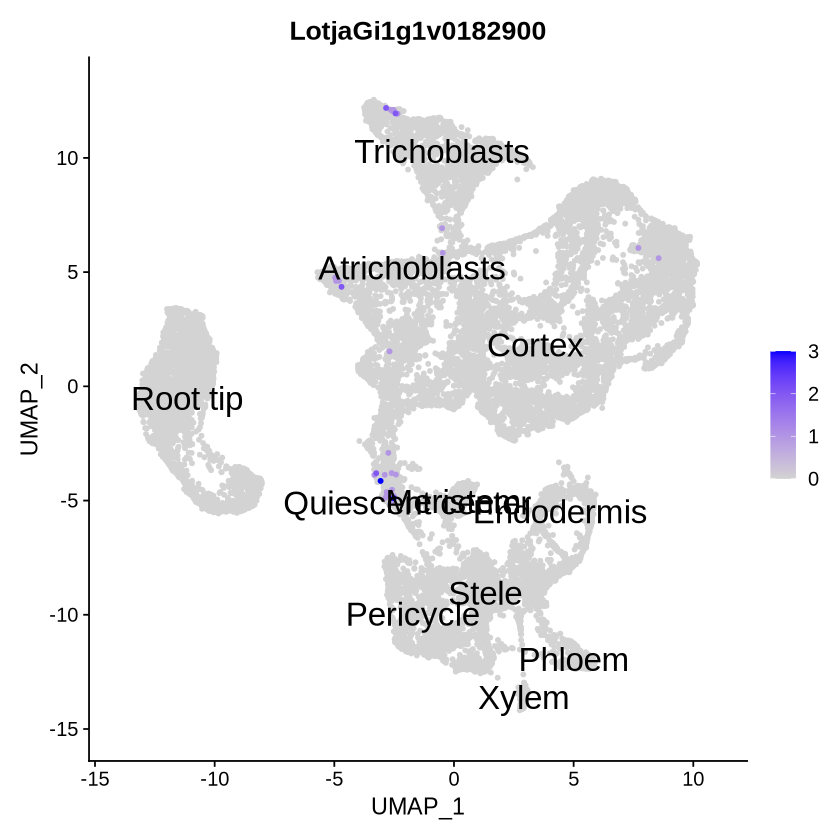
\includegraphics{tutorial-2024_files/figure-pdf/fig-rinrk-output-1.png}

}

\caption{\label{fig-rinrk}UMAP plot for the expression of gene RINRK1 in
the data}

\end{figure}%

From biological knowledge, we expect the gene mostly expressed in the
cortex and trichoblasts upon inoculation with rhizobia, and that is what
happens in our data as well. We can see it in the code and violin plot
of Figure~\ref{fig-vln}

\begin{Shaded}
\begin{Highlighting}[]
\FunctionTok{cat}\NormalTok{(}\StringTok{"Cells in inoculated L.J. expressing"}\NormalTok{, RINRK1.id, }\StringTok{"}\SpecialCharTok{\textbackslash{}n}\StringTok{"}\NormalTok{)}

\FunctionTok{cat}\NormalTok{( }\FunctionTok{sum}\NormalTok{( }\FunctionTok{as.numeric}\NormalTok{(}\FunctionTok{GetAssayData}\NormalTok{(seurat.clustered[RINRK1.id,]))}\SpecialCharTok{\textgreater{}}\DecValTok{0} \SpecialCharTok{\&} 
\NormalTok{     seurat.clustered}\SpecialCharTok{@}\NormalTok{meta.data}\SpecialCharTok{$}\NormalTok{Condition}\SpecialCharTok{==}\StringTok{"R7A"}\NormalTok{ ) )}

\FunctionTok{cat}\NormalTok{(}\StringTok{"}\SpecialCharTok{\textbackslash{}n}\StringTok{Cells in control L.J. expressing"}\NormalTok{, RINRK1.id, }\StringTok{"}\SpecialCharTok{\textbackslash{}n}\StringTok{"}\NormalTok{)}

\FunctionTok{cat}\NormalTok{( }\FunctionTok{sum}\NormalTok{( }\FunctionTok{as.numeric}\NormalTok{(}\FunctionTok{GetAssayData}\NormalTok{(seurat.clustered[RINRK1.id,]))}\SpecialCharTok{\textgreater{}}\DecValTok{0} \SpecialCharTok{\&} 
\NormalTok{    seurat.clustered}\SpecialCharTok{@}\NormalTok{meta.data}\SpecialCharTok{$}\NormalTok{Condition}\SpecialCharTok{==}\StringTok{"Control"}\NormalTok{ ) )}
\end{Highlighting}
\end{Shaded}

\begin{verbatim}
Cells in inoculated L.J. expressing LotjaGi1g1v0182900 
32
Cells in control L.J. expressing LotjaGi1g1v0182900 
0
\end{verbatim}

\begin{Shaded}
\begin{Highlighting}[]
\FunctionTok{VlnPlot}\NormalTok{(seurat.clustered, }
        \AttributeTok{features =}\NormalTok{ RINRK1.id)}
\end{Highlighting}
\end{Shaded}

\begin{figure}[H]

\centering{

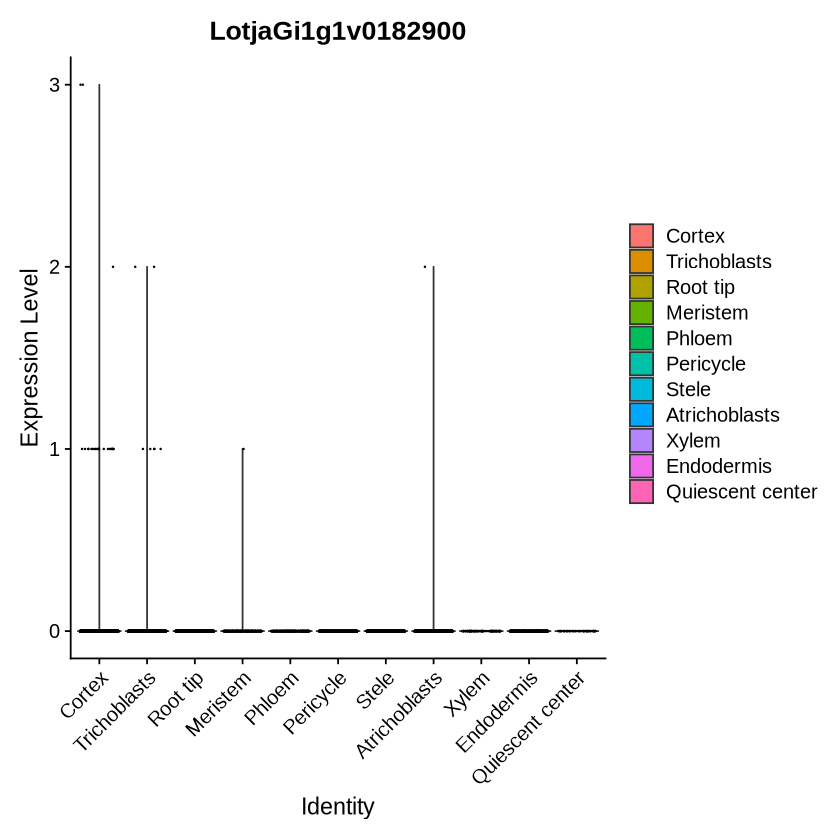
\includegraphics{tutorial-2024_files/figure-pdf/fig-vln-output-1.png}

}

\caption{\label{fig-vln}Violin plot for the expression of gene RINRK1 in
various clusters}

\end{figure}%

The code below uses \texttt{FindMarkers} to compare \texttt{R7A}
condition against \texttt{Control} for each cluster, with a filter to
remove non-singnificant genes (keeping p-value below 0.001 and log fold
change \textgreater{} 1 and \textless{} -1). We keep also genes
expressed 30\% more than in the condition where they are underexpressed.
We use only the 2000 most variable genes, since we are interested in
very variable gene expressions across data.

\begin{Shaded}
\begin{Highlighting}[]
\NormalTok{seurat.clustered }\OtherTok{\textless{}{-}} \FunctionTok{FindVariableFeatures}\NormalTok{(seurat.clustered, }\AttributeTok{nfeatures =} \DecValTok{2000}\NormalTok{, }\AttributeTok{assay =} \StringTok{"integrated"}\NormalTok{)}
\end{Highlighting}
\end{Shaded}

\begin{verbatim}
Warning message:
“Not all features provided are in this Assay object, removing the following feature(s): LotjaGi3g1v0268500, LotjaGi2g1v0180800, LotjaGi1g1v0192300, LotjaGi4g1v0383900, LotjaGi2g1v0178000, LotjaGi1g1v0748200, LotjaGi6g1v0166900-LC, LotjaGi6g1v0053200, LotjaGi2g1v0240800, LotjaGi1g1v0614900, LotjaGi1g1v0766800, LotjaGi1g1v0157700, LotjaGi2g1v0095600, LotjaGi1g1v0645700, LotjaGi1g1v0324300, LotjaGi5g1v0336700, LotjaGi6g1v0349200, LotjaGi3g1v0100600, LotjaGi1g1v0174500, LotjaGi2g1v0347900, LotjaGi2g1v0130600-LC, LotjaGi6g1v0167000-LC, LotjaGi3g1v0100400, LotjaGi3g1v0487600, LotjaGi1g1v0766200, LotjaGi5g1v0186200, LotjaGi3g1v0274700, LotjaGi2g1v0228100, LotjaGi1g1v0544500, LotjaGi5g1v0019000, LotjaGi3g1v0205900-LC, LotjaGi3g1v0150400, LotjaGi2g1v0000800, LotjaGi2g1v0177400, LotjaGi5g1v0178500, LotjaGi2g1v0005400, LotjaGi1g1v0667100, LotjaGi2g1v0435800, LotjaGi1g1v0320800, LotjaGi3g1v0222000, LotjaGi4g1v0392000, LotjaGi3g1v0114700, LotjaGi2g1v0143500, LotjaGi5g1v0013400, LotjaGi4g1v0452900, LotjaGi3g1v0468000, LotjaGi4g1v0193600-LC, LotjaGi4g1v0299200, LotjaGi4g1v0114900-LC, LotjaGi3g1v0178100, LotjaGi3g1v0050100, LotjaGi2g1v0176600, LotjaGi2g1v0183200, LotjaGi2g1v0081400, LotjaGi6g1v0271600, LotjaGi5g1v0169600, LotjaGi6g1v0012300-LC, LotjaGi2g1v0106500, LotjaGi3g1v0426100, LotjaGi6g1v0009600, LotjaGi1g1v0457800, LotjaGi4g1v0191000, LotjaGi5g1v0111200-LC, LotjaGi3g1v0526400-LC, LotjaGi6g1v0152400-LC, LotjaGi2g1v0246800, LotjaGi1g1v0798300, LotjaGi4g1v0152900, LotjaGi5g1v0082200, LotjaGi5g1v0118700, LotjaGi6g1v0197000, LotjaGi2g1v0291500, LotjaGi1g1v0692100, LotjaGi2g1v0424100, LotjaGi1g1v0636100, LotjaGi3g1v0147700-LC, LotjaGi5g1v0345000, LotjaGi5g1v0301600-LC, LotjaGi1g1v0026100, LotjaGi6g1v0166800, LotjaGi1g1v0776200, LotjaGi6g1v0086100, LotjaGi3g1v0381800, LotjaGi2g1v0121500, LotjaGi4g1v0091000, LotjaGi2g1v0093200, LotjaGi1g1v0768500-LC, LotjaGi1g1v0261000, LotjaGi2g1v0126400, LotjaGi1g1v0731900, LotjaGi3g1v0035700, LotjaGi2g1v0176900, LotjaGi3g1v0183200, LotjaGi2g1v0074700, LotjaGi2g1v0081200, LotjaGi2g1v0105800, LotjaGi1g1v0091300, LotjaGi5g1v0324600”
\end{verbatim}

\begin{Shaded}
\begin{Highlighting}[]
\NormalTok{DEG\_table }\OtherTok{\textless{}{-}} \FunctionTok{FindMarkers}\NormalTok{(seurat.clustered, }
                             \AttributeTok{assay=}\StringTok{\textquotesingle{}integrated\textquotesingle{}}\NormalTok{,}
                             \AttributeTok{ident.1 =} \StringTok{"R7A"}\NormalTok{,}
                             \AttributeTok{ident.2 =} \StringTok{"Control"}\NormalTok{, }
                             \AttributeTok{group.by =} \StringTok{"Condition"}\NormalTok{,}
                             \AttributeTok{subset.ident=}\StringTok{"Cortex"}\NormalTok{,}
                             \AttributeTok{min.diff.pct =} \FloatTok{0.3}\NormalTok{,}
                             \AttributeTok{verbose =} \ConstantTok{TRUE}\NormalTok{, }
                             \AttributeTok{features =}\NormalTok{ seurat.clustered}\SpecialCharTok{@}\NormalTok{assays}\SpecialCharTok{$}\NormalTok{integrated}\SpecialCharTok{@}\NormalTok{var.features,}
                             \AttributeTok{test.use =} \StringTok{"wilcox"}\NormalTok{) }\SpecialCharTok{\%\textgreater{}\%}
                             \FunctionTok{filter}\NormalTok{(p\_val\_adj }\SpecialCharTok{\textless{}=} \FloatTok{0.001} \SpecialCharTok{\&} \FunctionTok{abs}\NormalTok{(avg\_log2FC)}\SpecialCharTok{\textgreater{}}\DecValTok{1}\NormalTok{) }\SpecialCharTok{\%\textgreater{}\%}
                             \FunctionTok{select}\NormalTok{(}\SpecialCharTok{{-}}\NormalTok{p\_val)}
\end{Highlighting}
\end{Shaded}

\begin{Shaded}
\begin{Highlighting}[]
\FunctionTok{DefaultAssay}\NormalTok{(seurat.clustered) }\OtherTok{\textless{}{-}} \StringTok{"integrated"} \CommentTok{\#return to the integrated data}
\NormalTok{DEG }\OtherTok{\textless{}{-}} \FunctionTok{data.frame}\NormalTok{()}
\NormalTok{cluster.names }\OtherTok{\textless{}{-}} \FunctionTok{unique}\NormalTok{(}\FunctionTok{Idents}\NormalTok{(seurat.clustered))}

\ControlFlowTok{for}\NormalTok{(CLUSTER }\ControlFlowTok{in}\NormalTok{ cluster.names)\{}
\NormalTok{    DEG\_table }\OtherTok{\textless{}{-}} \FunctionTok{FindMarkers}\NormalTok{(seurat.clustered,}
                             \AttributeTok{assay=}\StringTok{\textquotesingle{}integrated\textquotesingle{}}\NormalTok{,}
                             \AttributeTok{ident.1 =} \StringTok{"R7A"}\NormalTok{,}
                             \AttributeTok{ident.2 =} \StringTok{"Control"}\NormalTok{, }
                             \AttributeTok{group.by =} \StringTok{"Condition"}\NormalTok{,}
                             \AttributeTok{subset.ident=}\NormalTok{CLUSTER,}
                             \AttributeTok{verbose =} \ConstantTok{TRUE}\NormalTok{, }
                             \AttributeTok{min.diff.pct =} \FloatTok{0.3}\NormalTok{,}
                             \AttributeTok{features =}\NormalTok{ seurat.clustered}\SpecialCharTok{@}\NormalTok{assays}\SpecialCharTok{$}\NormalTok{integrated}\SpecialCharTok{@}\NormalTok{var.features,}
                             \AttributeTok{test.use =} \StringTok{"wilcox"}\NormalTok{) }\SpecialCharTok{\%\textgreater{}\%}
                             \FunctionTok{filter}\NormalTok{(p\_val\_adj }\SpecialCharTok{\textless{}=} \FloatTok{0.001} \SpecialCharTok{\&} \FunctionTok{abs}\NormalTok{(avg\_log2FC)}\SpecialCharTok{\textgreater{}}\DecValTok{1}\NormalTok{) }\SpecialCharTok{\%\textgreater{}\%}
                             \FunctionTok{select}\NormalTok{(}\SpecialCharTok{{-}}\NormalTok{p\_val)}
    \ControlFlowTok{if}\NormalTok{(}\FunctionTok{dim}\NormalTok{(DEG\_table)[}\DecValTok{1}\NormalTok{]}\SpecialCharTok{\textgreater{}}\DecValTok{0}\NormalTok{)\{}
\NormalTok{        DEG\_table}\SpecialCharTok{$}\StringTok{\textquotesingle{}cluster\textquotesingle{}} \OtherTok{\textless{}{-}}\NormalTok{ CLUSTER}
\NormalTok{        DEG }\OtherTok{\textless{}{-}} \FunctionTok{rbind}\NormalTok{(DEG, DEG\_table)\}}
    \ControlFlowTok{else}\NormalTok{\{}
        \FunctionTok{message}\NormalTok{(}\FunctionTok{paste0}\NormalTok{(}\StringTok{"{-}{-}{-}\textgreater{} Warning: No DE genes in cluster "}\NormalTok{, CLUSTER), }\AttributeTok{appendLF=}\ConstantTok{FALSE}\NormalTok{)\}}
    \FunctionTok{message}\NormalTok{(}\FunctionTok{paste0}\NormalTok{(}\StringTok{"Done with cluster "}\NormalTok{,CLUSTER), }\AttributeTok{appendLF=}\ConstantTok{FALSE}\NormalTok{)}
\NormalTok{    \}}

\NormalTok{DEG }\OtherTok{\textless{}{-}} \FunctionTok{as.data.frame}\NormalTok{(DEG)}
\NormalTok{DEG}\SpecialCharTok{$}\NormalTok{gene }\OtherTok{\textless{}{-}} \FunctionTok{rownames}\NormalTok{(DEG)}
\end{Highlighting}
\end{Shaded}

\begin{verbatim}
Done with cluster Cortex
Done with cluster Trichoblasts
Done with cluster Root tip
Done with cluster Meristem
Done with cluster Phloem
Done with cluster Pericycle
Done with cluster Stele
Done with cluster Atrichoblasts
Done with cluster Xylem
Done with cluster Endodermis
---> Warning: No DE genes in cluster Quiescent center
Done with cluster Quiescent center
\end{verbatim}

The table looks like this. Columns represent:

\begin{itemize}
\tightlist
\item
  average logfoldchange between R7A and Control
\item
  percentage of cells in R7A expressing the gene
\item
  percentage of cells in Control expressing the gene
\item
  adjusted p-value
\item
  cluster
\item
  gene
\end{itemize}

There are some genes in the table

\begin{Shaded}
\begin{Highlighting}[]
\FunctionTok{dim}\NormalTok{(DEG)[}\DecValTok{1}\NormalTok{]}
\end{Highlighting}
\end{Shaded}

718

We now integrate GO terms

\begin{Shaded}
\begin{Highlighting}[]
\NormalTok{go\_table }\OtherTok{\textless{}{-}} \FunctionTok{read.table}\NormalTok{(}\StringTok{"./LJ\_GO\_terms.gaf"}\NormalTok{, }\AttributeTok{skip=}\DecValTok{6}\NormalTok{, }\AttributeTok{sep=}\StringTok{\textquotesingle{}}\SpecialCharTok{\textbackslash{}t}\StringTok{\textquotesingle{}}\NormalTok{, }\AttributeTok{fill=}\ConstantTok{TRUE}\NormalTok{, }\AttributeTok{quote =} \StringTok{"}\SpecialCharTok{\textbackslash{}"}\StringTok{"}\NormalTok{)}
\end{Highlighting}
\end{Shaded}

\begin{Shaded}
\begin{Highlighting}[]
\NormalTok{DEG }\OtherTok{\textless{}{-}} \FunctionTok{addGOterms}\NormalTok{(DEG, go\_table, }\AttributeTok{n.cores =} \DecValTok{16}\NormalTok{)}
\end{Highlighting}
\end{Shaded}

So we can see which GO terms are relevant in each cluster for the
infected samples against the control:

\begin{Shaded}
\begin{Highlighting}[]
\NormalTok{DEG }\SpecialCharTok{\%\textgreater{}\%} \FunctionTok{filter}\NormalTok{(cluster}\SpecialCharTok{==}\StringTok{"Cortex"} \SpecialCharTok{\&}\NormalTok{ GO}\SpecialCharTok{!=}\StringTok{"Undefined"}\NormalTok{)}
\end{Highlighting}
\end{Shaded}

A data.frame: 2 × 7

\begin{longtable}[]{@{}
  >{\raggedright\arraybackslash}p{(\columnwidth - 14\tabcolsep) * \real{0.1250}}
  >{\raggedright\arraybackslash}p{(\columnwidth - 14\tabcolsep) * \real{0.1250}}
  >{\raggedright\arraybackslash}p{(\columnwidth - 14\tabcolsep) * \real{0.1250}}
  >{\raggedright\arraybackslash}p{(\columnwidth - 14\tabcolsep) * \real{0.1250}}
  >{\raggedright\arraybackslash}p{(\columnwidth - 14\tabcolsep) * \real{0.1250}}
  >{\raggedright\arraybackslash}p{(\columnwidth - 14\tabcolsep) * \real{0.1250}}
  >{\raggedright\arraybackslash}p{(\columnwidth - 14\tabcolsep) * \real{0.1250}}
  >{\raggedright\arraybackslash}p{(\columnwidth - 14\tabcolsep) * \real{0.1250}}@{}}
\toprule\noalign{}
\begin{minipage}[b]{\linewidth}\raggedright
\end{minipage} & \begin{minipage}[b]{\linewidth}\raggedright
avg\_log2FC \textless dbl\textgreater{}
\end{minipage} & \begin{minipage}[b]{\linewidth}\raggedright
pct.1 \textless dbl\textgreater{}
\end{minipage} & \begin{minipage}[b]{\linewidth}\raggedright
pct.2 \textless dbl\textgreater{}
\end{minipage} & \begin{minipage}[b]{\linewidth}\raggedright
p\_val\_adj \textless dbl\textgreater{}
\end{minipage} & \begin{minipage}[b]{\linewidth}\raggedright
cluster \textless chr\textgreater{}
\end{minipage} & \begin{minipage}[b]{\linewidth}\raggedright
gene \textless chr\textgreater{}
\end{minipage} & \begin{minipage}[b]{\linewidth}\raggedright
GO \textless chr\textgreater{}
\end{minipage} \\
\midrule\noalign{}
\endhead
\bottomrule\noalign{}
\endlastfoot
LotjaGi1g1v0147200 & 5.757176 & 0.411 & 0.10 & 2.556740e-215 & Cortex &
LotjaGi1g1v0147200 & Trehalose 6-phosphate phosphatase; TAIR:
AT5G10100.1 Haloacid dehalogenase-like hydrolase (HAD) superfamily
protein; Swiss-Prot: sp \\
LotjaGi1g1v0154100 & 2.390368 & 0.422 & 0.12 & 2.637166e-97 & Cortex &
LotjaGi1g1v0154100 & Flavonol synthase; TAIR: AT5G08640.1 flavonol
synthase 1; Swiss-Prot: sp \\
\end{longtable}

Finally, we do not expect to find the RINRK1 gene as differentially
expressed, because its expression is on average too low.

\begin{Shaded}
\begin{Highlighting}[]
\NormalTok{DEG }\SpecialCharTok{\%\textgreater{}\%} \FunctionTok{filter}\NormalTok{(gene}\SpecialCharTok{==}\NormalTok{RINRK1.id)}
\end{Highlighting}
\end{Shaded}

A data.frame: 0 × 7

\begin{longtable}[]{@{}
  >{\raggedright\arraybackslash}p{(\columnwidth - 12\tabcolsep) * \real{0.1429}}
  >{\raggedright\arraybackslash}p{(\columnwidth - 12\tabcolsep) * \real{0.1429}}
  >{\raggedright\arraybackslash}p{(\columnwidth - 12\tabcolsep) * \real{0.1429}}
  >{\raggedright\arraybackslash}p{(\columnwidth - 12\tabcolsep) * \real{0.1429}}
  >{\raggedright\arraybackslash}p{(\columnwidth - 12\tabcolsep) * \real{0.1429}}
  >{\raggedright\arraybackslash}p{(\columnwidth - 12\tabcolsep) * \real{0.1429}}
  >{\raggedright\arraybackslash}p{(\columnwidth - 12\tabcolsep) * \real{0.1429}}@{}}
\toprule\noalign{}
\begin{minipage}[b]{\linewidth}\raggedright
avg\_log2FC \textless dbl\textgreater{}
\end{minipage} & \begin{minipage}[b]{\linewidth}\raggedright
pct.1 \textless dbl\textgreater{}
\end{minipage} & \begin{minipage}[b]{\linewidth}\raggedright
pct.2 \textless dbl\textgreater{}
\end{minipage} & \begin{minipage}[b]{\linewidth}\raggedright
p\_val\_adj \textless dbl\textgreater{}
\end{minipage} & \begin{minipage}[b]{\linewidth}\raggedright
cluster \textless chr\textgreater{}
\end{minipage} & \begin{minipage}[b]{\linewidth}\raggedright
gene \textless chr\textgreater{}
\end{minipage} & \begin{minipage}[b]{\linewidth}\raggedright
GO \textless chr\textgreater{}
\end{minipage} \\
\midrule\noalign{}
\endhead
\bottomrule\noalign{}
\endlastfoot
\end{longtable}

We save the table:

\begin{Shaded}
\begin{Highlighting}[]
\FunctionTok{write.csv}\NormalTok{(DEG\_table, }\StringTok{"DEG\_table.csv"}\NormalTok{)}
\end{Highlighting}
\end{Shaded}

\section{Coexpression analysis}\label{sec-networks}

We use the package hdWGCNA to detect groups of cells expressed
simultaneously, and we find which modules are differentially expressed
in specific clusters. We look at the GO terms to gain biological insight
in the data.

\begin{tcolorbox}[enhanced jigsaw, toprule=.15mm, coltitle=black, colframe=quarto-callout-note-color-frame, colback=white, colbacktitle=quarto-callout-note-color!10!white, opacityback=0, arc=.35mm, breakable, rightrule=.15mm, titlerule=0mm, leftrule=.75mm, bottomtitle=1mm, toptitle=1mm, title=\textcolor{quarto-callout-note-color}{\faInfo}\hspace{0.5em}{Note}, bottomrule=.15mm, left=2mm, opacitybacktitle=0.6]

Before running hdWGCNA, we first have to set up the Seurat object. Most
of the information computed by hdWGCNA will be stored in the Seurat
object's \texttt{@misc} slot.

\end{tcolorbox}

Here we will set up the Seurat object using the \texttt{SetupForWGCNA}
function, specifying the name of the \texttt{hdWGNCA} experiment. This
function also selects the genes that will be used for WGCNA. The user
can select genes using three different approaches using the posse
gene\_select parameter:

\begin{itemize}
\tightlist
\item
  variable: use the genes stored in the Seurat object's
  VariableFeatures.
\item
  fraction: use genes that are expressed in a certain fraction of cells
  for in the whole dataset or in each group of cells, specified by
  \texttt{group.by}.
\item
  custom: use genes that are specified in a custom list.
\end{itemize}

In this example, we will select genes that are expressed in at least 5\%
of cells in this dataset, and we will name our \texttt{hdWGCNA}
experiment ``tutorial''.

\begin{Shaded}
\begin{Highlighting}[]
\NormalTok{seurat.clustered }\OtherTok{\textless{}{-}} \FunctionTok{LoadH5Seurat}\NormalTok{(}\StringTok{"seurat.clustered.h5Seurat"}\NormalTok{, }\AttributeTok{verbose=}\ConstantTok{FALSE}\NormalTok{)}
\end{Highlighting}
\end{Shaded}

\begin{verbatim}
Validating h5Seurat file

Warning message:
“Adding a command log without an assay associated with it”
\end{verbatim}

\begin{Shaded}
\begin{Highlighting}[]
\NormalTok{seurat.clustered }\OtherTok{\textless{}{-}} \FunctionTok{SetupForWGCNA}\NormalTok{(}
\NormalTok{  seurat.clustered,}
  \AttributeTok{gene\_select =} \StringTok{"variable"}\NormalTok{,}
  \CommentTok{\#gene\_select = "fraction", \# the gene selection approach}
  \AttributeTok{fraction =} \FloatTok{0.05}\NormalTok{, }\CommentTok{\# fraction of cells that a gene needs to be expressed in order to be included}
  \AttributeTok{wgcna\_name =} \StringTok{"tutorial"} \CommentTok{\# the name of the hdWGCNA experiment}
\NormalTok{)}
\end{Highlighting}
\end{Shaded}

\subsection{Construct metacells}\label{construct-metacells}

After we have set up our Seurat object, the first step in running the
hdWGCNA pipeline is to construct metacells from the single-cell dataset.
Briefly, metacells are \textbf{aggregates of small groups of similar
cells originating from the same biological sample of origin}.

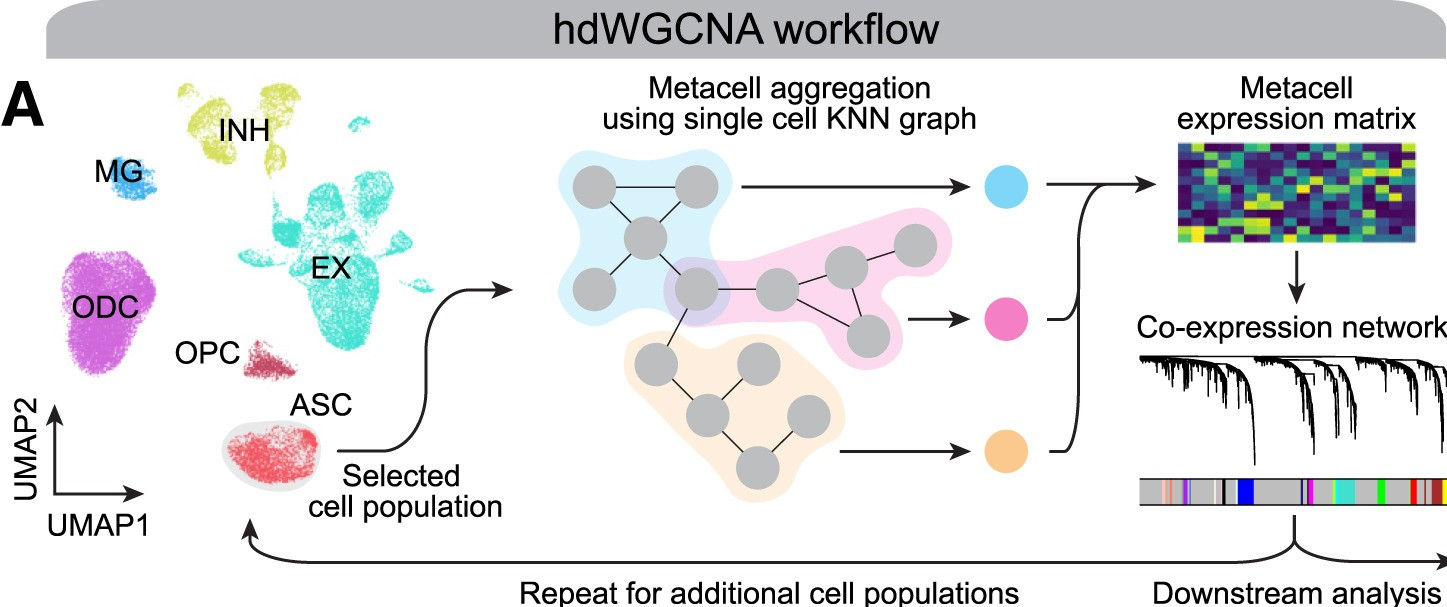
\includegraphics{./images/hdwgcna.jpg} \{\#fig-hdwgcna, width=800\}

\begin{tcolorbox}[enhanced jigsaw, toprule=.15mm, coltitle=black, colframe=quarto-callout-tip-color-frame, colback=white, colbacktitle=quarto-callout-tip-color!10!white, opacityback=0, arc=.35mm, breakable, rightrule=.15mm, titlerule=0mm, leftrule=.75mm, bottomtitle=1mm, toptitle=1mm, title=\textcolor{quarto-callout-tip-color}{\faLightbulb}\hspace{0.5em}{Something more about hdWGCNA}, bottomrule=.15mm, left=2mm, opacitybacktitle=0.6]

The k-Nearest Neighbors (KNN) algorithm is used to identify groups of
similar cells to aggregate, and then the average or summed expression of
these cells is computed, thus yielding a metacell gene expression matrix
(\textbf{as if you had many bulk samples}). The \textbf{sparsity of the
metacell expression matrix is considerably reduced} when compared to the
original expression matrix, and therefore it is preferable to use. We
were originally motivated to use metacells in place of the original
single cells because correlation \textbf{network approaches such as
WGCNA are sensitive to data sparsity}.

\texttt{hdWGCNA} includes a function \texttt{MetacellsByGroups} to
construct metacell expression matrices given a single-cell dataset. This
function constructs a new Seurat object for the metacell dataset which
is stored internally in the \texttt{hdWGCNA} experiment. The
\texttt{group.by} parameter determines which groups metacells will be
constructed in. We only want to construct metacells from cells that came
from the same biological sample of origin, so it is critical to pass
that information to \texttt{hdWGCNA} via the \texttt{group.by}
parameter. Additionally, we usually construct metacells for each cell
type separately. Thus, in this example, we are \textbf{grouping by
Sample and cell type} to achieve the desired result.

\textbf{The number of cells to be aggregated \texttt{k} should be tuned
based on the size of the input dataset}, in general a lower number for
\texttt{k} can be used for small datasets. We generally use \texttt{k}
values between 20 and 75. The dataset used for this tutorial has 21,369
cells, and here we use \texttt{k=20}. The amount of allowable overlap
between metacells can be tuned using the \texttt{max\_shared} argument.
There should be a range of \texttt{k} values that are suitable for
reducing the sparsity while retaining cellular heterogeneity for a given
dataset, rather than a single optimal value.

Note: the authors of \texttt{hdWGCNA} have found that the metacell
aggregation approach does not yield good results for extremely
underrepresented cell types. For example, in this dataset, the
\texttt{Meristem} and \texttt{Xylem} are the least represented, and will
be excluded them from this analysis. \texttt{MetacellsByGroups} has a
parameter \texttt{min\_cells} to exclude groups that are smaller than a
specified number of cells. \textbf{Errors are likely to arise if the
selected value for \texttt{min\_cells} is too low}.

\end{tcolorbox}

Here \textbf{we construct metacells and normalize the resulting
expression matrix} using the following code (read the additional text in
the box above to understand the parameters). Note how the clusters Xylem
and Quiescent center are removed, simply because they are too small and
cannot be used. So from now on we do not consider them for the
coexpression analysis.

\begin{Shaded}
\begin{Highlighting}[]
\CommentTok{\# construct metacells  in each group}
\NormalTok{seurat.clustered }\OtherTok{\textless{}{-}} \FunctionTok{MetacellsByGroups}\NormalTok{(}
  \AttributeTok{seurat\_obj =}\NormalTok{ seurat.clustered,}
  \AttributeTok{group.by =} \FunctionTok{c}\NormalTok{(}\StringTok{"predicted.id"}\NormalTok{, }\StringTok{"Condition"}\NormalTok{), }\CommentTok{\# specify metadata to split by cluster and condition}
  \AttributeTok{reduction =} \StringTok{\textquotesingle{}pca\textquotesingle{}}\NormalTok{, }\CommentTok{\# select the dimensionality reduction to perform KNN on}
  \AttributeTok{k =} \DecValTok{30}\NormalTok{, }\CommentTok{\# nearest{-}neighbors parameter}
  \AttributeTok{max\_shared =} \DecValTok{10}\NormalTok{, }\CommentTok{\# maximum number of shared cells between two metacells}
  \AttributeTok{ident.group =} \StringTok{\textquotesingle{}predicted.id\textquotesingle{}}\NormalTok{, }\CommentTok{\# set the Idents of the metacell seurat object}
  \AttributeTok{assay =} \StringTok{"integrated"}\NormalTok{,}
  \AttributeTok{slot =} \StringTok{"scale.data"}\NormalTok{,}
  \AttributeTok{min\_cells =} \DecValTok{100}\NormalTok{,}
  \AttributeTok{wgcna\_name =} \StringTok{"tutorial"}\NormalTok{,}
  \AttributeTok{verbose=}\ConstantTok{TRUE}
\NormalTok{)}
\end{Highlighting}
\end{Shaded}

\begin{verbatim}
Warning message in MetacellsByGroups(seurat_obj = seurat.clustered, group.by = c("predicted.id", :
“Removing the following groups that did not meet min_cells: Quiescent center#Control, Quiescent center#R7A, Xylem#Control, Xylem#R7A”
Overlap QC metrics:
Cells per bin: 30
Maximum shared cells bin-bin: 10
Mean shared cells bin-bin: 1.51461988304094
Median shared cells bin-bin: 0

Overlap QC metrics:
Cells per bin: 30
Maximum shared cells bin-bin: 10
Mean shared cells bin-bin: 0.635690485005553
Median shared cells bin-bin: 0

Overlap QC metrics:
Cells per bin: 30
Maximum shared cells bin-bin: 10
Mean shared cells bin-bin: 0.335219114968392
Median shared cells bin-bin: 0

Overlap QC metrics:
Cells per bin: 30
Maximum shared cells bin-bin: 10
Mean shared cells bin-bin: 0.19742043684862
Median shared cells bin-bin: 0

Overlap QC metrics:
Cells per bin: 30
Maximum shared cells bin-bin: 10
Mean shared cells bin-bin: 1.36752136752137
Median shared cells bin-bin: 0

Overlap QC metrics:
Cells per bin: 30
Maximum shared cells bin-bin: 10
Mean shared cells bin-bin: 1.59090909090909
Median shared cells bin-bin: 0

Overlap QC metrics:
Cells per bin: 30
Maximum shared cells bin-bin: 10
Mean shared cells bin-bin: 3.57575757575758
Median shared cells bin-bin: 2

Warning message in (function (seurat_obj, name = "agg", ident.group = "seurat_clusters", :
“On average, more than 10% of cells are shared between paired bins.”
Overlap QC metrics:
Cells per bin: 30
Maximum shared cells bin-bin: 9
Mean shared cells bin-bin: 4.66666666666667
Median shared cells bin-bin: 5

Warning message in (function (seurat_obj, name = "agg", ident.group = "seurat_clusters", :
“On average, more than 10% of cells are shared between paired bins.”
Overlap QC metrics:
Cells per bin: 30
Maximum shared cells bin-bin: 10
Mean shared cells bin-bin: 2.41578947368421
Median shared cells bin-bin: 0.5

Overlap QC metrics:
Cells per bin: 30
Maximum shared cells bin-bin: 10
Mean shared cells bin-bin: 1.13725490196078
Median shared cells bin-bin: 0

Overlap QC metrics:
Cells per bin: 30
Maximum shared cells bin-bin: 10
Mean shared cells bin-bin: 4.05555555555556
Median shared cells bin-bin: 3

Warning message in (function (seurat_obj, name = "agg", ident.group = "seurat_clusters", :
“On average, more than 10% of cells are shared between paired bins.”
Overlap QC metrics:
Cells per bin: 30
Maximum shared cells bin-bin: 9
Mean shared cells bin-bin: 3.9
Median shared cells bin-bin: 3

Warning message in (function (seurat_obj, name = "agg", ident.group = "seurat_clusters", :
“On average, more than 10% of cells are shared between paired bins.”
Overlap QC metrics:
Cells per bin: 30
Maximum shared cells bin-bin: 10
Mean shared cells bin-bin: 0.690802348336595
Median shared cells bin-bin: 0

Overlap QC metrics:
Cells per bin: 30
Maximum shared cells bin-bin: 10
Mean shared cells bin-bin: 0.659649122807018
Median shared cells bin-bin: 0

Overlap QC metrics:
Cells per bin: 30
Maximum shared cells bin-bin: 10
Mean shared cells bin-bin: 1.33547632963179
Median shared cells bin-bin: 0

Overlap QC metrics:
Cells per bin: 30
Maximum shared cells bin-bin: 10
Mean shared cells bin-bin: 0.9340592861464
Median shared cells bin-bin: 0

Overlap QC metrics:
Cells per bin: 30
Maximum shared cells bin-bin: 10
Mean shared cells bin-bin: 1.6312292358804
Median shared cells bin-bin: 0

Overlap QC metrics:
Cells per bin: 30
Maximum shared cells bin-bin: 10
Mean shared cells bin-bin: 0.77909604519774
Median shared cells bin-bin: 0
\end{verbatim}

\begin{Shaded}
\begin{Highlighting}[]
\CommentTok{\#normalize metacell expression matrix:}
\NormalTok{seurat.clustered }\OtherTok{\textless{}{-}} \FunctionTok{NormalizeMetacells}\NormalTok{(seurat.clustered)}
\end{Highlighting}
\end{Shaded}

\begin{verbatim}
Warning message:
“Cannot find a parent environment called Seurat”
\end{verbatim}

Here we specify the expression matrix that we will use for network
analysis. For example, we can choose the Cortex, which is important also
because it expresses RINRK1 in infected samples.

\begin{Shaded}
\begin{Highlighting}[]
\NormalTok{seurat.clustered }\OtherTok{\textless{}{-}} \FunctionTok{SetDatExpr}\NormalTok{(}
\NormalTok{  seurat.clustered,}
  \AttributeTok{group\_name =} \FunctionTok{c}\NormalTok{(}\StringTok{\textquotesingle{}Pericycle\textquotesingle{}}\NormalTok{,}\StringTok{\textquotesingle{}Cortex\textquotesingle{}}\NormalTok{,}\StringTok{\textquotesingle{}Trichoblasts\textquotesingle{}}\NormalTok{,}\StringTok{\textquotesingle{}Root tip\textquotesingle{}}\NormalTok{,}
                 \StringTok{\textquotesingle{}Phloem\textquotesingle{}}\NormalTok{,}\StringTok{\textquotesingle{}Stele\textquotesingle{}}\NormalTok{,}\StringTok{\textquotesingle{}Endodermis\textquotesingle{}}\NormalTok{,}\StringTok{\textquotesingle{}Atrichoblasts\textquotesingle{}}\NormalTok{,}
                 \StringTok{\textquotesingle{}Meristem\textquotesingle{}}\NormalTok{), }\CommentTok{\#all groups of interest in the data (we use all clusters)}
  \AttributeTok{group.by=}\StringTok{\textquotesingle{}predicted.id\textquotesingle{}}\NormalTok{, }\CommentTok{\# the metadata column containing the cell type info. This same column should have also been used in MetacellsByGroups}
  \AttributeTok{assay =} \StringTok{\textquotesingle{}integrated\textquotesingle{}}\NormalTok{, }\CommentTok{\# using integrated assay}
  \AttributeTok{slot =} \StringTok{\textquotesingle{}counts\textquotesingle{}} \CommentTok{\# using count data}
\NormalTok{)}
\end{Highlighting}
\end{Shaded}

\subsection{Select soft-power
threshold}\label{select-soft-power-threshold}

Next we will select the soft power threshold. This is an extremely
important step in the pipeline. \texttt{hdWGCNA} constructs a gene-gene
correlation adjacency matrix to infer co-expression relationships
between genes. The correlations are \textbf{raised to a power to reduce
the amount of noise present in the correlation matrix}, thereby
\textbf{retaining the strong connections and removing the weak
connections}. Therefore, it is critical to determine a proper value for
the soft power threshold.

We use the function \texttt{TestSoftPowers} to perform a parameter sweep
for different soft power thresholds. This function helps us to guide our
choice in a soft power threshold for constructing the co-expression
network by inspecting the resulting network topology for different power
values. The following code performs the parameter sweep and outputs a
summary figure.

\begin{Shaded}
\begin{Highlighting}[]
\CommentTok{\# Test different soft powers:}
\NormalTok{seurat.clustered }\OtherTok{\textless{}{-}} \FunctionTok{TestSoftPowers}\NormalTok{(}\AttributeTok{powers =} \DecValTok{1}\SpecialCharTok{:}\DecValTok{100}\NormalTok{,}
\NormalTok{  seurat.clustered,}
  \AttributeTok{networkType =} \StringTok{\textquotesingle{}signed\textquotesingle{}}
\NormalTok{)}

\CommentTok{\# plot the results:}
\NormalTok{plot\_list }\OtherTok{\textless{}{-}} \FunctionTok{PlotSoftPowers}\NormalTok{(seurat.clustered)}

\CommentTok{\# assemble with patchwork}
\FunctionTok{wrap\_plots}\NormalTok{(plot\_list, }\AttributeTok{ncol=}\DecValTok{2}\NormalTok{)}
\end{Highlighting}
\end{Shaded}

\begin{verbatim}
pickSoftThreshold: will use block size 1902.
 pickSoftThreshold: calculating connectivity for given powers...
   ..working on genes 1 through 1902 of 1902
    Power SFT.R.sq  slope truncated.R.sq  mean.k. median.k.   max.k.
1       1   0.7870  6.540         0.8230 1.14e+03  1.16e+03 1330.000
2       2   0.5050  2.320         0.7630 7.07e+02  7.28e+02  964.000
3       3   0.0603  0.528         0.6600 4.49e+02  4.62e+02  718.000
4       4   0.0241 -0.281         0.7740 2.91e+02  2.97e+02  548.000
5       5   0.2060 -0.780         0.9000 1.93e+02  1.93e+02  426.000
6       6   0.4090 -1.180         0.9510 1.30e+02  1.27e+02  338.000
7       7   0.5580 -1.460         0.9780 8.97e+01  8.48e+01  272.000
8       8   0.6540 -1.620         0.9910 6.27e+01  5.72e+01  222.000
9       9   0.7350 -1.740         0.9970 4.46e+01  3.87e+01  184.000
10     10   0.7830 -1.830         0.9810 3.22e+01  2.65e+01  153.000
11     11   0.8250 -1.890         0.9740 2.35e+01  1.81e+01  130.000
12     12   0.8580 -1.960         0.9810 1.74e+01  1.25e+01  110.000
13     13   0.8600 -2.020         0.9540 1.31e+01  8.80e+00   94.700
14     14   0.8390 -2.080         0.9060 9.96e+00  6.18e+00   81.800
15     15   0.8500 -2.070         0.9010 7.65e+00  4.37e+00   71.200
16     16   0.9030 -2.020         0.9560 5.94e+00  3.11e+00   62.400
17     17   0.8950 -2.030         0.9480 4.66e+00  2.24e+00   54.900
18     18   0.9090 -1.990         0.9560 3.69e+00  1.61e+00   48.600
19     19   0.9080 -1.970         0.9440 2.95e+00  1.16e+00   43.200
20     20   0.8770 -1.990         0.8950 2.37e+00  8.56e-01   38.500
21     21   0.8810 -1.960         0.8940 1.93e+00  6.31e-01   34.500
22     22   0.8930 -1.930         0.9030 1.57e+00  4.67e-01   31.100
23     23   0.9020 -1.900         0.9100 1.30e+00  3.41e-01   28.000
24     24   0.3400 -2.670         0.1990 1.07e+00  2.55e-01   25.400
25     25   0.3390 -2.620         0.1970 8.94e-01  1.89e-01   23.100
26     26   0.3420 -2.580         0.2000 7.50e-01  1.41e-01   21.000
27     27   0.3460 -2.540         0.2050 6.32e-01  1.05e-01   19.200
28     28   0.3480 -2.510         0.2080 5.35e-01  8.04e-02   17.600
29     29   0.3540 -2.490         0.2170 4.55e-01  6.06e-02   16.100
30     30   0.3530 -2.450         0.2170 3.89e-01  4.56e-02   14.800
31     31   0.3820 -2.500         0.3120 3.35e-01  3.53e-02   13.700
32     32   0.3200 -2.220         0.1280 2.89e-01  2.73e-02   12.600
33     33   0.3210 -2.190         0.1290 2.50e-01  2.08e-02   11.700
34     34   0.3220 -2.160         0.1310 2.17e-01  1.61e-02   10.900
35     35   0.3240 -2.140         0.1330 1.90e-01  1.25e-02   10.100
36     36   0.3260 -2.120         0.1350 1.66e-01  9.64e-03    9.400
37     37   0.3280 -2.090         0.1380 1.46e-01  7.42e-03    8.770
38     38   0.3280 -2.070         0.1390 1.29e-01  5.78e-03    8.200
39     39   0.3290 -2.040         0.1400 1.14e-01  4.42e-03    7.670
40     40   0.2780 -2.410         0.0721 1.01e-01  3.42e-03    7.190
41     41   0.2790 -2.380         0.0744 9.01e-02  2.64e-03    6.740
42     42   0.2790 -2.370         0.0737 8.05e-02  2.07e-03    6.340
43     43   0.2800 -2.340         0.0745 7.21e-02  1.62e-03    5.960
44     44   0.2810 -2.320         0.0757 6.47e-02  1.26e-03    5.620
45     45   0.2810 -2.310         0.0765 5.83e-02  1.00e-03    5.300
46     46   0.2830 -2.290         0.0784 5.26e-02  7.83e-04    5.010
47     47   0.3010 -2.320         0.1050 4.76e-02  6.10e-04    4.740
48     48   0.3000 -2.290         0.1040 4.32e-02  4.74e-04    4.480
49     49   0.2990 -2.270         0.1040 3.93e-02  3.75e-04    4.250
50     50   0.3030 -2.250         0.1090 3.58e-02  2.99e-04    4.030
51     51   0.3040 -2.230         0.1110 3.27e-02  2.39e-04    3.830
52     52   0.3050 -2.210         0.1120 2.99e-02  1.91e-04    3.640
53     53   0.3060 -2.200         0.1140 2.74e-02  1.51e-04    3.460
54     54   0.2920 -2.420         0.0894 2.52e-02  1.19e-04    3.300
55     55   0.2920 -2.400         0.0896 2.32e-02  9.27e-05    3.140
56     56   0.2930 -2.390         0.0906 2.14e-02  7.35e-05    3.000
57     57   0.2950 -2.370         0.0933 1.98e-02  5.97e-05    2.860
58     58   0.2960 -2.340         0.0947 1.83e-02  4.85e-05    2.730
59     59   0.2970 -2.320         0.0963 1.70e-02  3.86e-05    2.610
60     60   0.2980 -2.310         0.0981 1.58e-02  3.09e-05    2.500
61     61   0.2970 -2.290         0.0969 1.47e-02  2.46e-05    2.390
62     62   0.2990 -2.270         0.0994 1.37e-02  1.94e-05    2.290
63     63   0.2990 -2.250         0.0994 1.28e-02  1.54e-05    2.200
64     64   0.3010 -2.230         0.1020 1.19e-02  1.22e-05    2.110
65     65   0.3000 -2.220         0.1010 1.12e-02  9.72e-06    2.020
66     66   0.3010 -2.210         0.1020 1.05e-02  7.74e-06    1.940
67     67   0.3030 -2.200         0.1040 9.81e-03  6.17e-06    1.860
68     68   0.3040 -2.190         0.1060 9.22e-03  4.95e-06    1.790
69     69   0.3050 -2.180         0.1080 8.67e-03  3.99e-06    1.730
70     70   0.3190 -2.210         0.1310 8.16e-03  3.25e-06    1.660
71     71   0.3200 -2.200         0.1340 7.70e-03  2.58e-06    1.600
72     72   0.2990 -2.270         0.1080 7.26e-03  2.03e-06    1.550
73     73   0.2980 -2.260         0.1060 6.86e-03  1.62e-06    1.490
74     74   0.3000 -2.240         0.1080 6.49e-03  1.31e-06    1.440
75     75   0.3020 -2.230         0.1090 6.14e-03  1.08e-06    1.390
76     76   0.3040 -2.220         0.1110 5.82e-03  8.57e-07    1.350
77     77   0.3030 -2.210         0.1100 5.52e-03  6.87e-07    1.300
78     78   0.3050 -2.200         0.1110 5.24e-03  5.63e-07    1.260
79     79   0.3050 -2.180         0.1110 4.97e-03  4.58e-07    1.220
80     80   0.3040 -2.180         0.1100 4.73e-03  3.69e-07    1.180
81     81   0.3030 -2.190         0.1080 4.50e-03  2.97e-07    1.150
82     82   0.3030 -2.170         0.1080 4.28e-03  2.38e-07    1.110
83     83   0.3020 -2.150         0.1080 4.08e-03  1.90e-07    1.080
84     84   0.3040 -2.150         0.1090 3.89e-03  1.51e-07    1.040
85     85   0.3050 -2.140         0.1110 3.72e-03  1.20e-07    1.010
86     86   0.3070 -2.130         0.1120 3.55e-03  9.65e-08    0.982
87     87   0.3080 -2.120         0.1140 3.39e-03  7.71e-08    0.953
88     88   0.3090 -2.130         0.1150 3.24e-03  6.29e-08    0.926
89     89   0.3100 -2.140         0.1160 3.10e-03  5.03e-08    0.899
90     90   0.3110 -2.140         0.1170 2.97e-03  4.04e-08    0.874
91     91   0.3130 -2.130         0.1190 2.85e-03  3.23e-08    0.849
92     92   0.3140 -2.120         0.1200 2.73e-03  2.58e-08    0.826
93     93   0.3150 -2.130         0.1220 2.62e-03  2.08e-08    0.803
94     94   0.3270 -2.160         0.1350 2.51e-03  1.70e-08    0.781
95     95   0.3290 -2.150         0.1370 2.41e-03  1.40e-08    0.760
96     96   0.3300 -2.140         0.1390 2.32e-03  1.15e-08    0.740
97     97   0.3300 -2.130         0.1390 2.23e-03  9.37e-09    0.720
98     98   0.3320 -2.120         0.1410 2.14e-03  7.61e-09    0.701
99     99   0.3400 -2.130         0.1540 2.06e-03  6.14e-09    0.683
100   100   0.3410 -2.120         0.1550 1.98e-03  4.95e-09    0.666
  Power   SFT.R.sq      slope truncated.R.sq   mean.k. median.k.    max.k.
1     1 0.78715066  6.5419434      0.8226937 1142.8616 1164.8542 1330.4551
2     2 0.50547179  2.3222895      0.7627136  706.9821  727.8092  963.5889
3     3 0.06030832  0.5277599      0.6599972  448.5438  461.6084  717.8182
4     4 0.02406336 -0.2805631      0.7737510  291.1354  296.5913  547.5911
5     5 0.20640114 -0.7801742      0.9004039  192.9425  193.3074  426.3568
6     6 0.40937211 -1.1838404      0.9509733  130.3530  127.1297  337.9309
\end{verbatim}

\begin{verbatim}
Warning message:
“executing %dopar% sequentially: no parallel backend registered”
\end{verbatim}

\begin{figure}[H]

\centering{

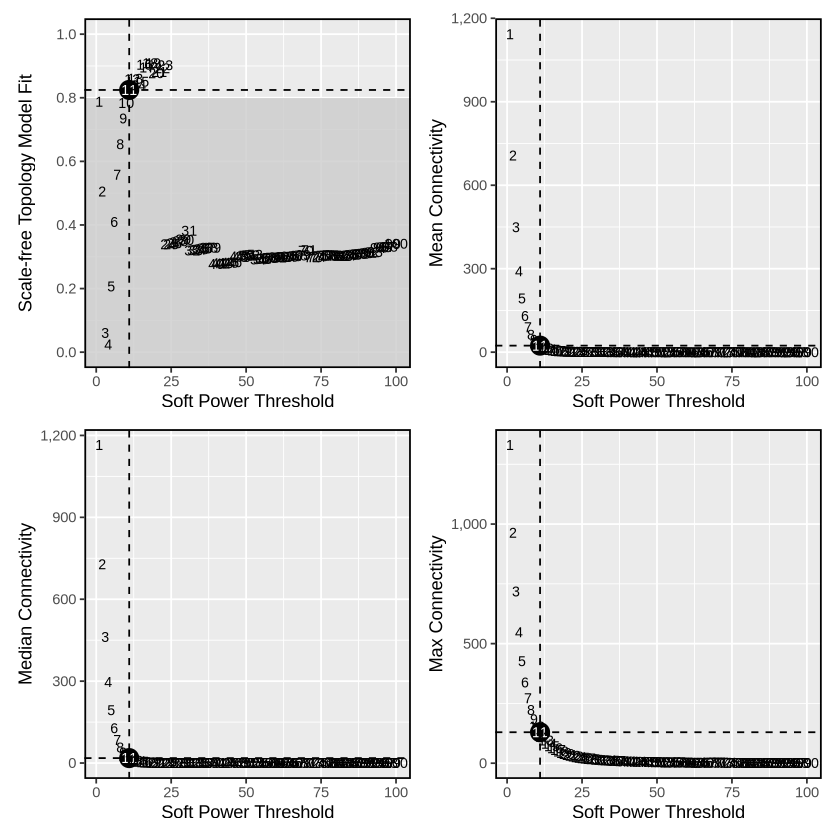
\includegraphics{tutorial-2024_files/figure-pdf/fig-sweep-output-3.png}

}

\caption{\label{fig-sweep}Parameter sweep to choose the soft power
threshold}

\end{figure}%

The general guidance for \texttt{hdWGCNA} is to pick the lowest soft
power threshold that has Model Fit greater than or equal to 0.8, so in
this case we would select our soft power threshold to be 11 following
the illustration fo Figure~\ref{fig-sweep}. Later on, the
\texttt{ConstructNetwork} command will automatically select the soft
power threshold if the user does not provide one.

\subsection{Construction of co-expression
network}\label{construction-of-co-expression-network}

We now have everything that we need to construct our co-expression
network. Here we use the \texttt{hdWGCNA} function
\texttt{ConstructNetwork}. This function has quite a few parameters to
play with if you are an advanced user (read
\href{https://rdrr.io/github/smorabit/hdWGCNA/man/ConstructNetwork.html}{this
manual} and the function \texttt{ConstructNetwork} is based on
\href{https://www.rdocumentation.org/packages/WGCNA/versions/1.72-5/topics/blockwiseConsensusModules}{here}),
but we use default parameters that work well with many single-cell
datasets.

The following code constructs the co-expression network using the soft
power threshold selected before:

\begin{Shaded}
\begin{Highlighting}[]
\CommentTok{\# construct co{-}expression network:}
\NormalTok{seurat.clustered }\OtherTok{\textless{}{-}} \FunctionTok{ConstructNetwork}\NormalTok{(}\AttributeTok{na.rm=}\ConstantTok{TRUE}\NormalTok{,}
\NormalTok{  seurat.clustered,}
  \AttributeTok{soft\_power=}\DecValTok{11}\NormalTok{,                                   }
  \AttributeTok{setDatExpr=}\ConstantTok{FALSE}\NormalTok{,}
  \AttributeTok{tom\_name =} \StringTok{\textquotesingle{}Cortex\textquotesingle{}}\NormalTok{, }\CommentTok{\# name of the topoligical overlap matrix written to disk}
  \AttributeTok{overwrite\_tom =} \ConstantTok{TRUE}
\NormalTok{)}
\end{Highlighting}
\end{Shaded}

\begin{verbatim}
Warning message in ConstructNetwork(na.rm = TRUE, seurat.clustered, soft_power = 11, :
“Overwriting TOM TOM/Cortex_TOM.rda”
\end{verbatim}

\begin{verbatim}
 Calculating consensus modules and module eigengenes block-wise from all genes
 Calculating topological overlaps block-wise from all genes
   Flagging genes and samples with too many missing values...
    ..step 1
    TOM calculation: adjacency..
    ..will not use multithreading.
     Fraction of slow calculations: 0.000000
    ..connectivity..
    ..matrix multiplication (system BLAS)..
    ..normalization..
    ..done.
 ..Working on block 1 .
 ..Working on block 1 .
 ..merging consensus modules that are too close..
\end{verbatim}

We can plot the network dendrogram in Figure~\ref{fig-dendro}. Each leaf
on the dendrogram represents a single gene, and the color at the bottom
indicates the co-expression module assignment.

\textbf{Note: the ``gray'' module consists of genes that were not
grouped into any co-expression module. The gray module is to be ignored
for all downstream analysis and interpretation.}

\begin{Shaded}
\begin{Highlighting}[]
\FunctionTok{PlotDendrogram}\NormalTok{(seurat.clustered, }\AttributeTok{main=}\StringTok{\textquotesingle{}Phloem hdWGCNA Dendrogram\textquotesingle{}}\NormalTok{)}
\end{Highlighting}
\end{Shaded}

\begin{figure}[H]

\centering{

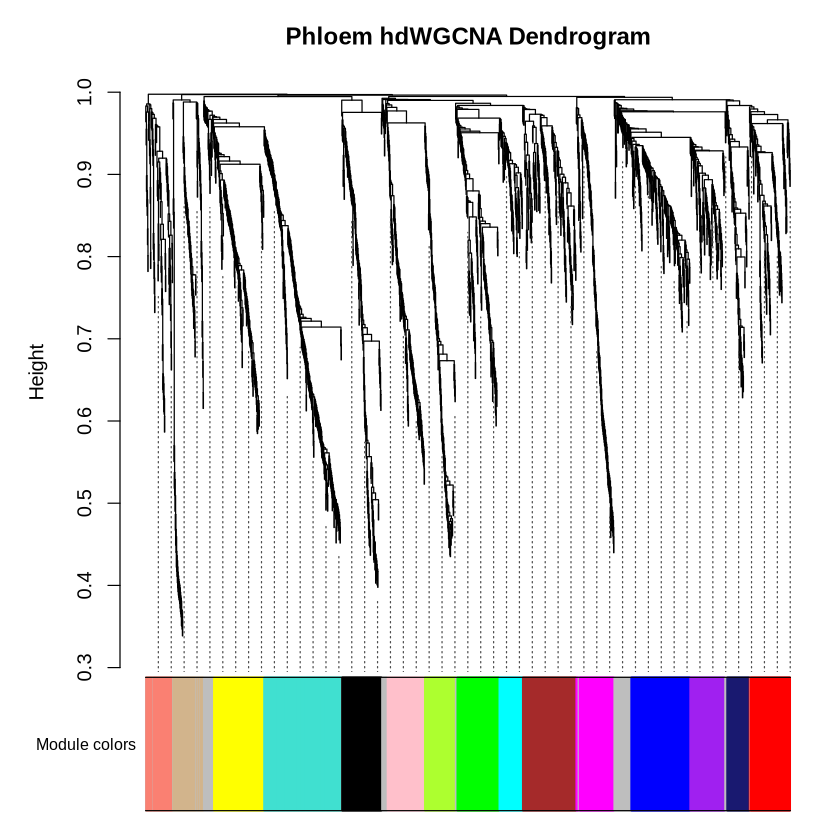
\includegraphics{tutorial-2024_files/figure-pdf/fig-dendro-output-1.png}

}

\caption{\label{fig-dendro}Dendrogram of the genes coexpression network.
Leaves at the bottom are genes, and the colours represent a module of
coexpression for the corresponding genes. Gray areas are for genes not
included in any module.}

\end{figure}%

\subsubsection{Module Eigengenes (MEs)}\label{module-eigengenes-mes}

We calculate harmonized module eigengenes. This is a way of doing PCA of
the expression matrix of metacells including the genes of one
coexpression module at a time. Thus we have a PCA of the data for each
module. The first principal component of each PCA is called module
eigengene: it is enough to distinguish one module from all the others
and characterize the expression pattern of the module (Langfelder and
Horvath (2007))!

Dimensionality reduction techniques are a very hot topic in single-cell
genomics (Xiang et al. (2021)). It is well known that technical
artifacts can muddy the analysis of single-cell datasets, and over the
years there have been many methods that aim to reduce the effects of
these artifacts. Therefore it stands to reason that MEs would be subject
to these technical artifacts as well, and \texttt{hdWGCNA} seeks to
alleviate these effects by using the integration software
\texttt{Harmony} (Korsunsky et al. (2019)).

The following code performs the module eigengene computation harmonizing
by the Sample of origin using the \texttt{group.by.vars} parameter.

\begin{Shaded}
\begin{Highlighting}[]
\CommentTok{\# need to run ScaleData first or else harmony throws an error:}
\NormalTok{seurat.clustered }\OtherTok{\textless{}{-}} \FunctionTok{ScaleData}\NormalTok{(seurat.clustered, }
                              \AttributeTok{features=}\FunctionTok{VariableFeatures}\NormalTok{(seurat.clustered), }
                              \AttributeTok{verbose =} \ConstantTok{FALSE}\NormalTok{)}
\end{Highlighting}
\end{Shaded}

\begin{Shaded}
\begin{Highlighting}[]
\CommentTok{\# compute all MEs in the full single{-}cell dataset}
\NormalTok{seurat.clustered }\OtherTok{\textless{}{-}} \FunctionTok{ModuleEigengenes}\NormalTok{( }
\NormalTok{ seurat.clustered,}
 \AttributeTok{group.by.vars=}\StringTok{"orig.ident"}\NormalTok{,}
 \AttributeTok{verbose =} \ConstantTok{FALSE}
\NormalTok{)}
\end{Highlighting}
\end{Shaded}

\begin{verbatim}
[1] "turquoise"
[1] "brown"
[1] "salmon"
[1] "black"
[1] "red"
[1] "midnightblue"
[1] "magenta"
[1] "yellow"
[1] "blue"
[1] "green"
[1] "cyan"
[1] "grey"
[1] "greenyellow"
[1] "tan"
[1] "pink"
[1] "purple"
\end{verbatim}

\begin{verbatim}
Centering and scaling data matrix

Warning message:
“Keys should be one or more alphanumeric characters followed by an underscore, setting key from pcaturquoise to pcaturquoise_”
Centering and scaling data matrix

Warning message:
“Keys should be one or more alphanumeric characters followed by an underscore, setting key from pcabrown to pcabrown_”
Warning message:
“Key ‘harmony_’ taken, using ‘lsmpe_’ instead”
Centering and scaling data matrix

Warning message in irlba(A = t(x = object), nv = npcs, ...):
“You're computing too large a percentage of total singular values, use a standard svd instead.”
Warning message:
“Keys should be one or more alphanumeric characters followed by an underscore, setting key from pcasalmon to pcasalmon_”
Centering and scaling data matrix

Warning message:
“Keys should be one or more alphanumeric characters followed by an underscore, setting key from pcablack to pcablack_”
Warning message:
“Key ‘harmony_’ taken, using ‘nibyo_’ instead”
Centering and scaling data matrix

Warning message:
“Keys should be one or more alphanumeric characters followed by an underscore, setting key from pcared to pcared_”
Centering and scaling data matrix

Warning message in irlba(A = t(x = object), nv = npcs, ...):
“You're computing too large a percentage of total singular values, use a standard svd instead.”
Warning message:
“Keys should be one or more alphanumeric characters followed by an underscore, setting key from pcamidnightblue to pcamidnightblue_”
Warning message:
“Key ‘harmony_’ taken, using ‘lkzye_’ instead”
Centering and scaling data matrix

Warning message:
“Keys should be one or more alphanumeric characters followed by an underscore, setting key from pcamagenta to pcamagenta_”
Centering and scaling data matrix

Warning message:
“Keys should be one or more alphanumeric characters followed by an underscore, setting key from pcayellow to pcayellow_”
Warning message:
“Key ‘harmony_’ taken, using ‘ltnwf_’ instead”
Centering and scaling data matrix

Warning message:
“Keys should be one or more alphanumeric characters followed by an underscore, setting key from pcablue to pcablue_”
Centering and scaling data matrix

Warning message:
“Keys should be one or more alphanumeric characters followed by an underscore, setting key from pcagreen to pcagreen_”
Warning message:
“Key ‘harmony_’ taken, using ‘xolrz_’ instead”
Centering and scaling data matrix

Warning message in irlba(A = t(x = object), nv = npcs, ...):
“You're computing too large a percentage of total singular values, use a standard svd instead.”
Warning message:
“Keys should be one or more alphanumeric characters followed by an underscore, setting key from pcacyan to pcacyan_”
Centering and scaling data matrix

Warning message:
“Keys should be one or more alphanumeric characters followed by an underscore, setting key from pcagrey to pcagrey_”
Warning message:
“Key ‘harmony_’ taken, using ‘ibzol_’ instead”
Centering and scaling data matrix

Warning message in irlba(A = t(x = object), nv = npcs, ...):
“You're computing too large a percentage of total singular values, use a standard svd instead.”
Warning message:
“Keys should be one or more alphanumeric characters followed by an underscore, setting key from pcagreenyellow to pcagreenyellow_”
Centering and scaling data matrix

Warning message in irlba(A = t(x = object), nv = npcs, ...):
“You're computing too large a percentage of total singular values, use a standard svd instead.”
Warning message:
“Keys should be one or more alphanumeric characters followed by an underscore, setting key from pcatan to pcatan_”
Warning message:
“Key ‘harmony_’ taken, using ‘pical_’ instead”
Centering and scaling data matrix

Warning message:
“Keys should be one or more alphanumeric characters followed by an underscore, setting key from pcapink to pcapink_”
Centering and scaling data matrix

Warning message:
“Keys should be one or more alphanumeric characters followed by an underscore, setting key from pcapurple to pcapurple_”
Warning message:
“Key ‘harmony_’ taken, using ‘vnltp_’ instead”
\end{verbatim}

\subsubsection{Compute module
connectivity}\label{compute-module-connectivity}

In co-expression network analysis, we often want to focus on the
\textbf{hub genes, those which are highly connected within each module}.
Therefore we wish to determine the eigengene-based connectivity, also
known as kME, of each gene. The \texttt{ModuleConnectivity} function
computes the kMEs in the single-cell dataset (rather than the metacell
dataset). This function essentially computes pairwise correlations
between genes and module eigengenes. kME can be computed for all cells
in the dataset, but it is recommended computing kMEs in the cell type(s)
or group(s) previously used to run \texttt{ConstructNetwork}.

\begin{Shaded}
\begin{Highlighting}[]
\CommentTok{\# compute eigengene{-}based connectivity (kME):}
\NormalTok{seurat.clustered }\OtherTok{\textless{}{-}} \FunctionTok{ModuleConnectivity}\NormalTok{(}
\NormalTok{  seurat.clustered,}
  \AttributeTok{group.by =} \StringTok{\textquotesingle{}predicted.id\textquotesingle{}}\NormalTok{, }
  \AttributeTok{group\_name =} \FunctionTok{c}\NormalTok{(}\StringTok{\textquotesingle{}Pericycle\textquotesingle{}}\NormalTok{,}\StringTok{\textquotesingle{}Cortex\textquotesingle{}}\NormalTok{,}\StringTok{\textquotesingle{}Trichoblasts\textquotesingle{}}\NormalTok{,}\StringTok{\textquotesingle{}Root tip\textquotesingle{}}\NormalTok{,}
                 \StringTok{\textquotesingle{}Phloem\textquotesingle{}}\NormalTok{,}\StringTok{\textquotesingle{}Stele\textquotesingle{}}\NormalTok{,}\StringTok{\textquotesingle{}Endodermis\textquotesingle{}}\NormalTok{,}\StringTok{\textquotesingle{}Atrichoblasts\textquotesingle{}}\NormalTok{,}
                 \StringTok{\textquotesingle{}Meristem\textquotesingle{}}\NormalTok{,}\StringTok{\textquotesingle{}Xylem\textquotesingle{}}\NormalTok{),}
\NormalTok{)}
\end{Highlighting}
\end{Shaded}

For convenience, we re-name the hdWGCNA modules to indicate that they
are from the Cortex cluster.

\begin{Shaded}
\begin{Highlighting}[]
\CommentTok{\# rename the modules}
\NormalTok{seurat.clustered }\OtherTok{\textless{}{-}} \FunctionTok{ResetModuleNames}\NormalTok{(}
\NormalTok{  seurat.clustered,}
  \AttributeTok{new\_name =} \StringTok{"Lotus{-}Mod"}
\NormalTok{)}
\end{Highlighting}
\end{Shaded}

We can visualize the genes in each module ranked by kME using the
\texttt{PlotKMEs} function.

\begin{Shaded}
\begin{Highlighting}[]
\FunctionTok{options}\NormalTok{(}\AttributeTok{repr.plot.width=}\DecValTok{20}\NormalTok{, }\AttributeTok{repr.plot.height=}\DecValTok{25}\NormalTok{)}
\NormalTok{p }\OtherTok{\textless{}{-}} \FunctionTok{capture.output}\NormalTok{(\{}\FunctionTok{PlotKMEs}\NormalTok{(seurat.clustered, }\AttributeTok{ncol=}\DecValTok{3}\NormalTok{, }\AttributeTok{text\_size =} \DecValTok{4}\NormalTok{);\})}
\end{Highlighting}
\end{Shaded}

\begin{figure}[H]

\centering{

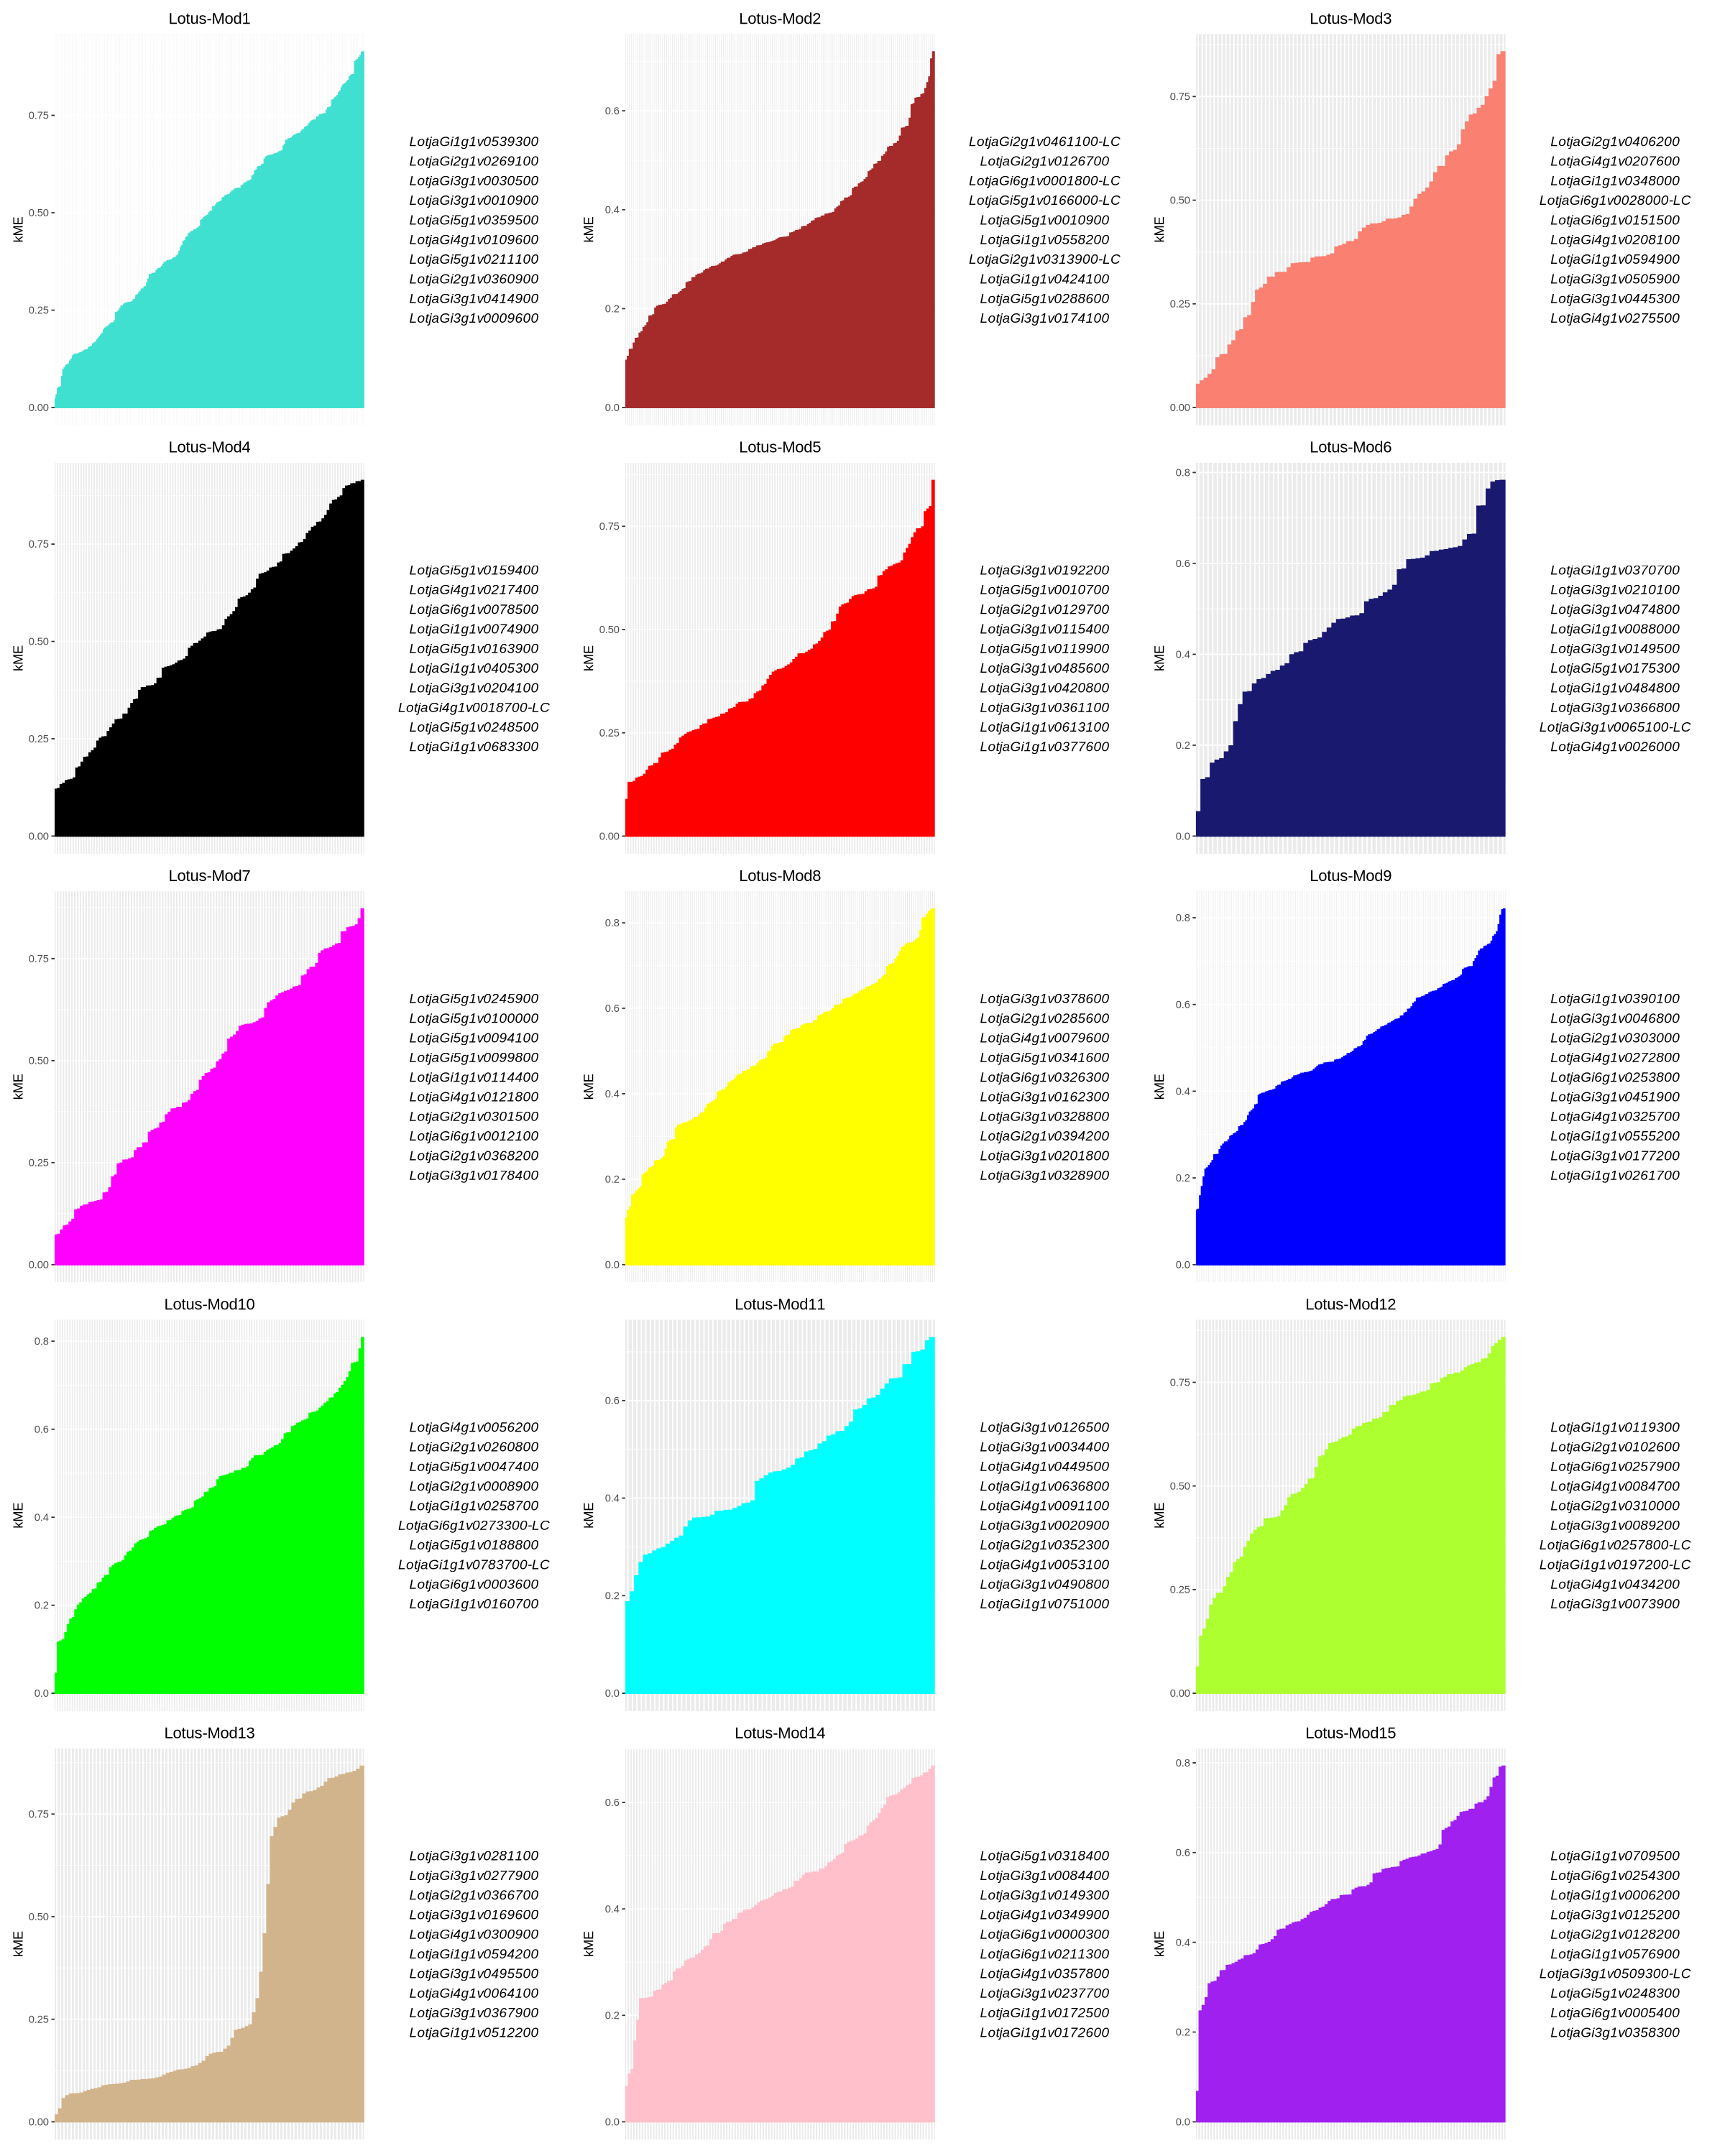
\includegraphics{tutorial-2024_files/figure-pdf/fig-kme-output-1.png}

}

\caption{\label{fig-kme}KMEs for each module, where the genes on the
right of each plot gives the top genes based on the module's KMEs. Each
plot is a histogram which has been rotated, so that bars starting on the
left side of the y axis represent the counts of how many genes have the
connectivity written on the right side of the y axis. The number of
counts should be written on the x axis, but is not plotted by the
function.}

\end{figure}%

\subsubsection{Getting the module assignment
table}\label{getting-the-module-assignment-table}

The plots of Figure~\ref{fig-kme} are a bit hard to read, though fancy
to plot. \texttt{hdWGCNA} allows for easy access of the module
assignment table using the \texttt{GetModules} function. This table
consists of three columns: \texttt{gene\_name} stores the gene's symbol
or ID, module stores the gene's module assignment, and color stores a
color mapping for each module (which is used in plotting steps). If
\texttt{ModuleConnectivity} has been used on this hdWGCNA experiment, as
it is our case, this table has additional columns with the
connectivities plotted in Figure~\ref{fig-kme}

\begin{Shaded}
\begin{Highlighting}[]
\CommentTok{\# get the module assignment table:}
\NormalTok{modules }\OtherTok{\textless{}{-}} \FunctionTok{GetModules}\NormalTok{(seurat.clustered)}

\CommentTok{\# show the first 6 columns:}
\FunctionTok{head}\NormalTok{(modules[,}\DecValTok{1}\SpecialCharTok{:}\DecValTok{6}\NormalTok{])}
\end{Highlighting}
\end{Shaded}

A data.frame: 6 × 6

\begin{longtable}[]{@{}
  >{\raggedright\arraybackslash}p{(\columnwidth - 12\tabcolsep) * \real{0.1429}}
  >{\raggedright\arraybackslash}p{(\columnwidth - 12\tabcolsep) * \real{0.1429}}
  >{\raggedright\arraybackslash}p{(\columnwidth - 12\tabcolsep) * \real{0.1429}}
  >{\raggedright\arraybackslash}p{(\columnwidth - 12\tabcolsep) * \real{0.1429}}
  >{\raggedright\arraybackslash}p{(\columnwidth - 12\tabcolsep) * \real{0.1429}}
  >{\raggedright\arraybackslash}p{(\columnwidth - 12\tabcolsep) * \real{0.1429}}
  >{\raggedright\arraybackslash}p{(\columnwidth - 12\tabcolsep) * \real{0.1429}}@{}}
\toprule\noalign{}
\begin{minipage}[b]{\linewidth}\raggedright
\end{minipage} & \begin{minipage}[b]{\linewidth}\raggedright
gene\_name \textless chr\textgreater{}
\end{minipage} & \begin{minipage}[b]{\linewidth}\raggedright
module \textless fct\textgreater{}
\end{minipage} & \begin{minipage}[b]{\linewidth}\raggedright
color \textless chr\textgreater{}
\end{minipage} & \begin{minipage}[b]{\linewidth}\raggedright
kME\_Lotus-Mod1 \textless dbl\textgreater{}
\end{minipage} & \begin{minipage}[b]{\linewidth}\raggedright
kME\_Lotus-Mod2 \textless dbl\textgreater{}
\end{minipage} & \begin{minipage}[b]{\linewidth}\raggedright
kME\_Lotus-Mod3 \textless dbl\textgreater{}
\end{minipage} \\
\midrule\noalign{}
\endhead
\bottomrule\noalign{}
\endlastfoot
LotjaGi3g1v0321700 & LotjaGi3g1v0321700 & Lotus-Mod1 & turquoise &
0.8397488 & -0.1355572 & -0.2505539 \\
LotjaGi2g1v0360900 & LotjaGi2g1v0360900 & Lotus-Mod1 & turquoise &
0.9035133 & -0.1649301 & -0.2914684 \\
LotjaGi3g1v0506700 & LotjaGi3g1v0506700 & Lotus-Mod1 & turquoise &
0.7470380 & -0.1574194 & -0.2274758 \\
LotjaGi3g1v0222100 & LotjaGi3g1v0222100 & Lotus-Mod2 & brown &
-0.1650440 & 0.4451741 & -0.1961163 \\
LotjaGi3g1v0445300 & LotjaGi3g1v0445300 & Lotus-Mod3 & salmon &
-0.2402357 & -0.1797755 & 0.8505632 \\
LotjaGi6g1v0155800 & LotjaGi6g1v0155800 & Lotus-Mod1 & turquoise &
0.7323678 & -0.1353630 & -0.2581496 \\
\end{longtable}

A table of the top N hub genes sorted by kME can be extracted using the
\texttt{GetHubGenes} function. Here we choose the top 10 genes, but you
can change the value if you want

\begin{Shaded}
\begin{Highlighting}[]
\CommentTok{\# get hub genes}
\NormalTok{hub\_df }\OtherTok{\textless{}{-}} \FunctionTok{GetHubGenes}\NormalTok{(seurat.clustered, }\AttributeTok{n\_hubs =} \DecValTok{10}\NormalTok{)}

\FunctionTok{head}\NormalTok{( hub\_df )}
\end{Highlighting}
\end{Shaded}

A data.frame: 6 × 3

\begin{longtable}[]{@{}
  >{\raggedright\arraybackslash}p{(\columnwidth - 6\tabcolsep) * \real{0.2500}}
  >{\raggedright\arraybackslash}p{(\columnwidth - 6\tabcolsep) * \real{0.2500}}
  >{\raggedright\arraybackslash}p{(\columnwidth - 6\tabcolsep) * \real{0.2500}}
  >{\raggedright\arraybackslash}p{(\columnwidth - 6\tabcolsep) * \real{0.2500}}@{}}
\toprule\noalign{}
\begin{minipage}[b]{\linewidth}\raggedright
\end{minipage} & \begin{minipage}[b]{\linewidth}\raggedright
gene\_name \textless chr\textgreater{}
\end{minipage} & \begin{minipage}[b]{\linewidth}\raggedright
module \textless fct\textgreater{}
\end{minipage} & \begin{minipage}[b]{\linewidth}\raggedright
kME \textless dbl\textgreater{}
\end{minipage} \\
\midrule\noalign{}
\endhead
\bottomrule\noalign{}
\endlastfoot
1 & LotjaGi1g1v0539300 & Lotus-Mod1 & 0.8522461 \\
2 & LotjaGi2g1v0269100 & Lotus-Mod1 & 0.8544151 \\
3 & LotjaGi3g1v0030500 & Lotus-Mod1 & 0.8551061 \\
4 & LotjaGi3g1v0010900 & Lotus-Mod1 & 0.8877517 \\
5 & LotjaGi5g1v0359500 & Lotus-Mod1 & 0.8911171 \\
6 & LotjaGi4g1v0109600 & Lotus-Mod1 & 0.8935191 \\
\end{longtable}

Again, we can assign GO terms to better check associated functions

\begin{Shaded}
\begin{Highlighting}[]
\NormalTok{go\_table }\OtherTok{\textless{}{-}} \FunctionTok{read.table}\NormalTok{(}\StringTok{"./LJ\_GO\_terms.gaf"}\NormalTok{, }\AttributeTok{skip=}\DecValTok{6}\NormalTok{, }\AttributeTok{sep=}\StringTok{\textquotesingle{}}\SpecialCharTok{\textbackslash{}t}\StringTok{\textquotesingle{}}\NormalTok{, }\AttributeTok{fill=}\ConstantTok{TRUE}\NormalTok{, }\AttributeTok{quote =} \StringTok{"}\SpecialCharTok{\textbackslash{}"}\StringTok{"}\NormalTok{)}
\end{Highlighting}
\end{Shaded}

\begin{Shaded}
\begin{Highlighting}[]
\NormalTok{hub\_df }\OtherTok{\textless{}{-}} \FunctionTok{addGOterms}\NormalTok{(}\AttributeTok{input\_table =}\NormalTok{ hub\_df, }
                     \AttributeTok{go\_table =}\NormalTok{ go\_table, }
                     \AttributeTok{gene\_column =} \StringTok{\textquotesingle{}gene\_name\textquotesingle{}}\NormalTok{,}
                     \AttributeTok{n.cores =} \DecValTok{16}\NormalTok{)}
\end{Highlighting}
\end{Shaded}

Now it is easy to look at each module and relevant GO terms.

\begin{Shaded}
\begin{Highlighting}[]
\NormalTok{hub\_filtered }\OtherTok{\textless{}{-}}\NormalTok{ hub\_df }\SpecialCharTok{\%\textgreater{}\%} \FunctionTok{filter}\NormalTok{(module }\SpecialCharTok{==} \StringTok{"Lotus{-}Mod3"}\NormalTok{)}
\end{Highlighting}
\end{Shaded}

\begin{Shaded}
\begin{Highlighting}[]
\NormalTok{hub\_filtered}
\end{Highlighting}
\end{Shaded}

A data.frame: 10 × 4

\begin{longtable}[]{@{}
  >{\raggedright\arraybackslash}p{(\columnwidth - 6\tabcolsep) * \real{0.2500}}
  >{\raggedright\arraybackslash}p{(\columnwidth - 6\tabcolsep) * \real{0.2500}}
  >{\raggedright\arraybackslash}p{(\columnwidth - 6\tabcolsep) * \real{0.2500}}
  >{\raggedright\arraybackslash}p{(\columnwidth - 6\tabcolsep) * \real{0.2500}}@{}}
\toprule\noalign{}
\begin{minipage}[b]{\linewidth}\raggedright
gene\_name \textless chr\textgreater{}
\end{minipage} & \begin{minipage}[b]{\linewidth}\raggedright
module \textless fct\textgreater{}
\end{minipage} & \begin{minipage}[b]{\linewidth}\raggedright
kME \textless dbl\textgreater{}
\end{minipage} & \begin{minipage}[b]{\linewidth}\raggedright
GO \textless chr\textgreater{}
\end{minipage} \\
\midrule\noalign{}
\endhead
\bottomrule\noalign{}
\endlastfoot
LotjaGi2g1v0406200 & Lotus-Mod3 & 0.6885007 & Undefined \\
LotjaGi4g1v0207600 & Lotus-Mod3 & 0.7048991 & Undefined \\
LotjaGi1g1v0348000 & Lotus-Mod3 & 0.7078898 & Aspartic proteinase
nepenthesin-1; TAIR: AT1G09750.1 Eukaryotic aspartyl protease family
protein; Swiss-Prot: sp \\
LotjaGi6g1v0028000-LC & Lotus-Mod3 & 0.7213880 & Undefined \\
LotjaGi6g1v0151500 & Lotus-Mod3 & 0.7284848 & Undefined \\
LotjaGi4g1v0208100 & Lotus-Mod3 & 0.7491915 & Undefined \\
LotjaGi1g1v0594900 & Lotus-Mod3 & 0.7680713 & Undefined \\
LotjaGi3g1v0505900 & Lotus-Mod3 & 0.7862156 & Undefined \\
LotjaGi3g1v0445300 & Lotus-Mod3 & 0.8505632 & Undefined \\
LotjaGi4g1v0275500 & Lotus-Mod3 & 0.8577066 & Undefined \\
\end{longtable}

We save the table for later use

\begin{Shaded}
\begin{Highlighting}[]
\FunctionTok{write.csv}\NormalTok{(hub\_df, }\StringTok{"top\_genes\_networks.csv"}\NormalTok{)}
\end{Highlighting}
\end{Shaded}

We can also plot the modules to see where they are most relevant on the
UMAP plot. First we calculate the scores of each module.

\begin{Shaded}
\begin{Highlighting}[]
\NormalTok{features\_list }\OtherTok{\textless{}{-}} \FunctionTok{list}\NormalTok{()}

\ControlFlowTok{for}\NormalTok{(MOD }\ControlFlowTok{in}\NormalTok{ hub\_df}\SpecialCharTok{$}\NormalTok{module)\{}
\NormalTok{    genes }\OtherTok{\textless{}{-}}\NormalTok{ hub\_df }\SpecialCharTok{\%\textgreater{}\%} \FunctionTok{filter}\NormalTok{(module }\SpecialCharTok{==}\NormalTok{ MOD)}
\NormalTok{    genes\_mod }\OtherTok{\textless{}{-}}\NormalTok{ genes}\SpecialCharTok{$}\NormalTok{gene\_name}
\NormalTok{    features\_list[[MOD]] }\OtherTok{\textless{}{-}}\NormalTok{ genes\_mod}
\NormalTok{    \}}

\NormalTok{seurat.clustered }\OtherTok{\textless{}{-}} \FunctionTok{AddModuleScore}\NormalTok{(}
  \AttributeTok{object =}\NormalTok{ seurat.clustered,}
  \AttributeTok{features =}\NormalTok{ features\_list,}
  \AttributeTok{ctrl =} \DecValTok{5}\NormalTok{,}
\NormalTok{)}

\NormalTok{seurat.clustered }\OtherTok{\textless{}{-}} \FunctionTok{renameScores}\NormalTok{(}\AttributeTok{markers\_list =}\NormalTok{ features\_list, }\AttributeTok{seurat\_data =}\NormalTok{ seurat.clustered)}
\FunctionTok{plotScoresUMAP}\NormalTok{(}\AttributeTok{markers\_list =}\NormalTok{ features\_list, }\AttributeTok{seurat\_data =}\NormalTok{ seurat.clustered)}
\end{Highlighting}
\end{Shaded}

\begin{verbatim}
Scores renamed FROM




TO



\end{verbatim}

\begin{verbatim}
Cluster1
Cluster2
Cluster3
Cluster4
Cluster5
Cluster6
Cluster7
Cluster8
Cluster9
Cluster10
Cluster11
Cluster12
Cluster13
Cluster14
Cluster15
Lotus-Mod1
Lotus-Mod2
Lotus-Mod3
Lotus-Mod4
Lotus-Mod5
Lotus-Mod6
Lotus-Mod7
Lotus-Mod8
Lotus-Mod9
Lotus-Mod10
Lotus-Mod11
Lotus-Mod12
Lotus-Mod13
Lotus-Mod14
Lotus-Mod15
\end{verbatim}

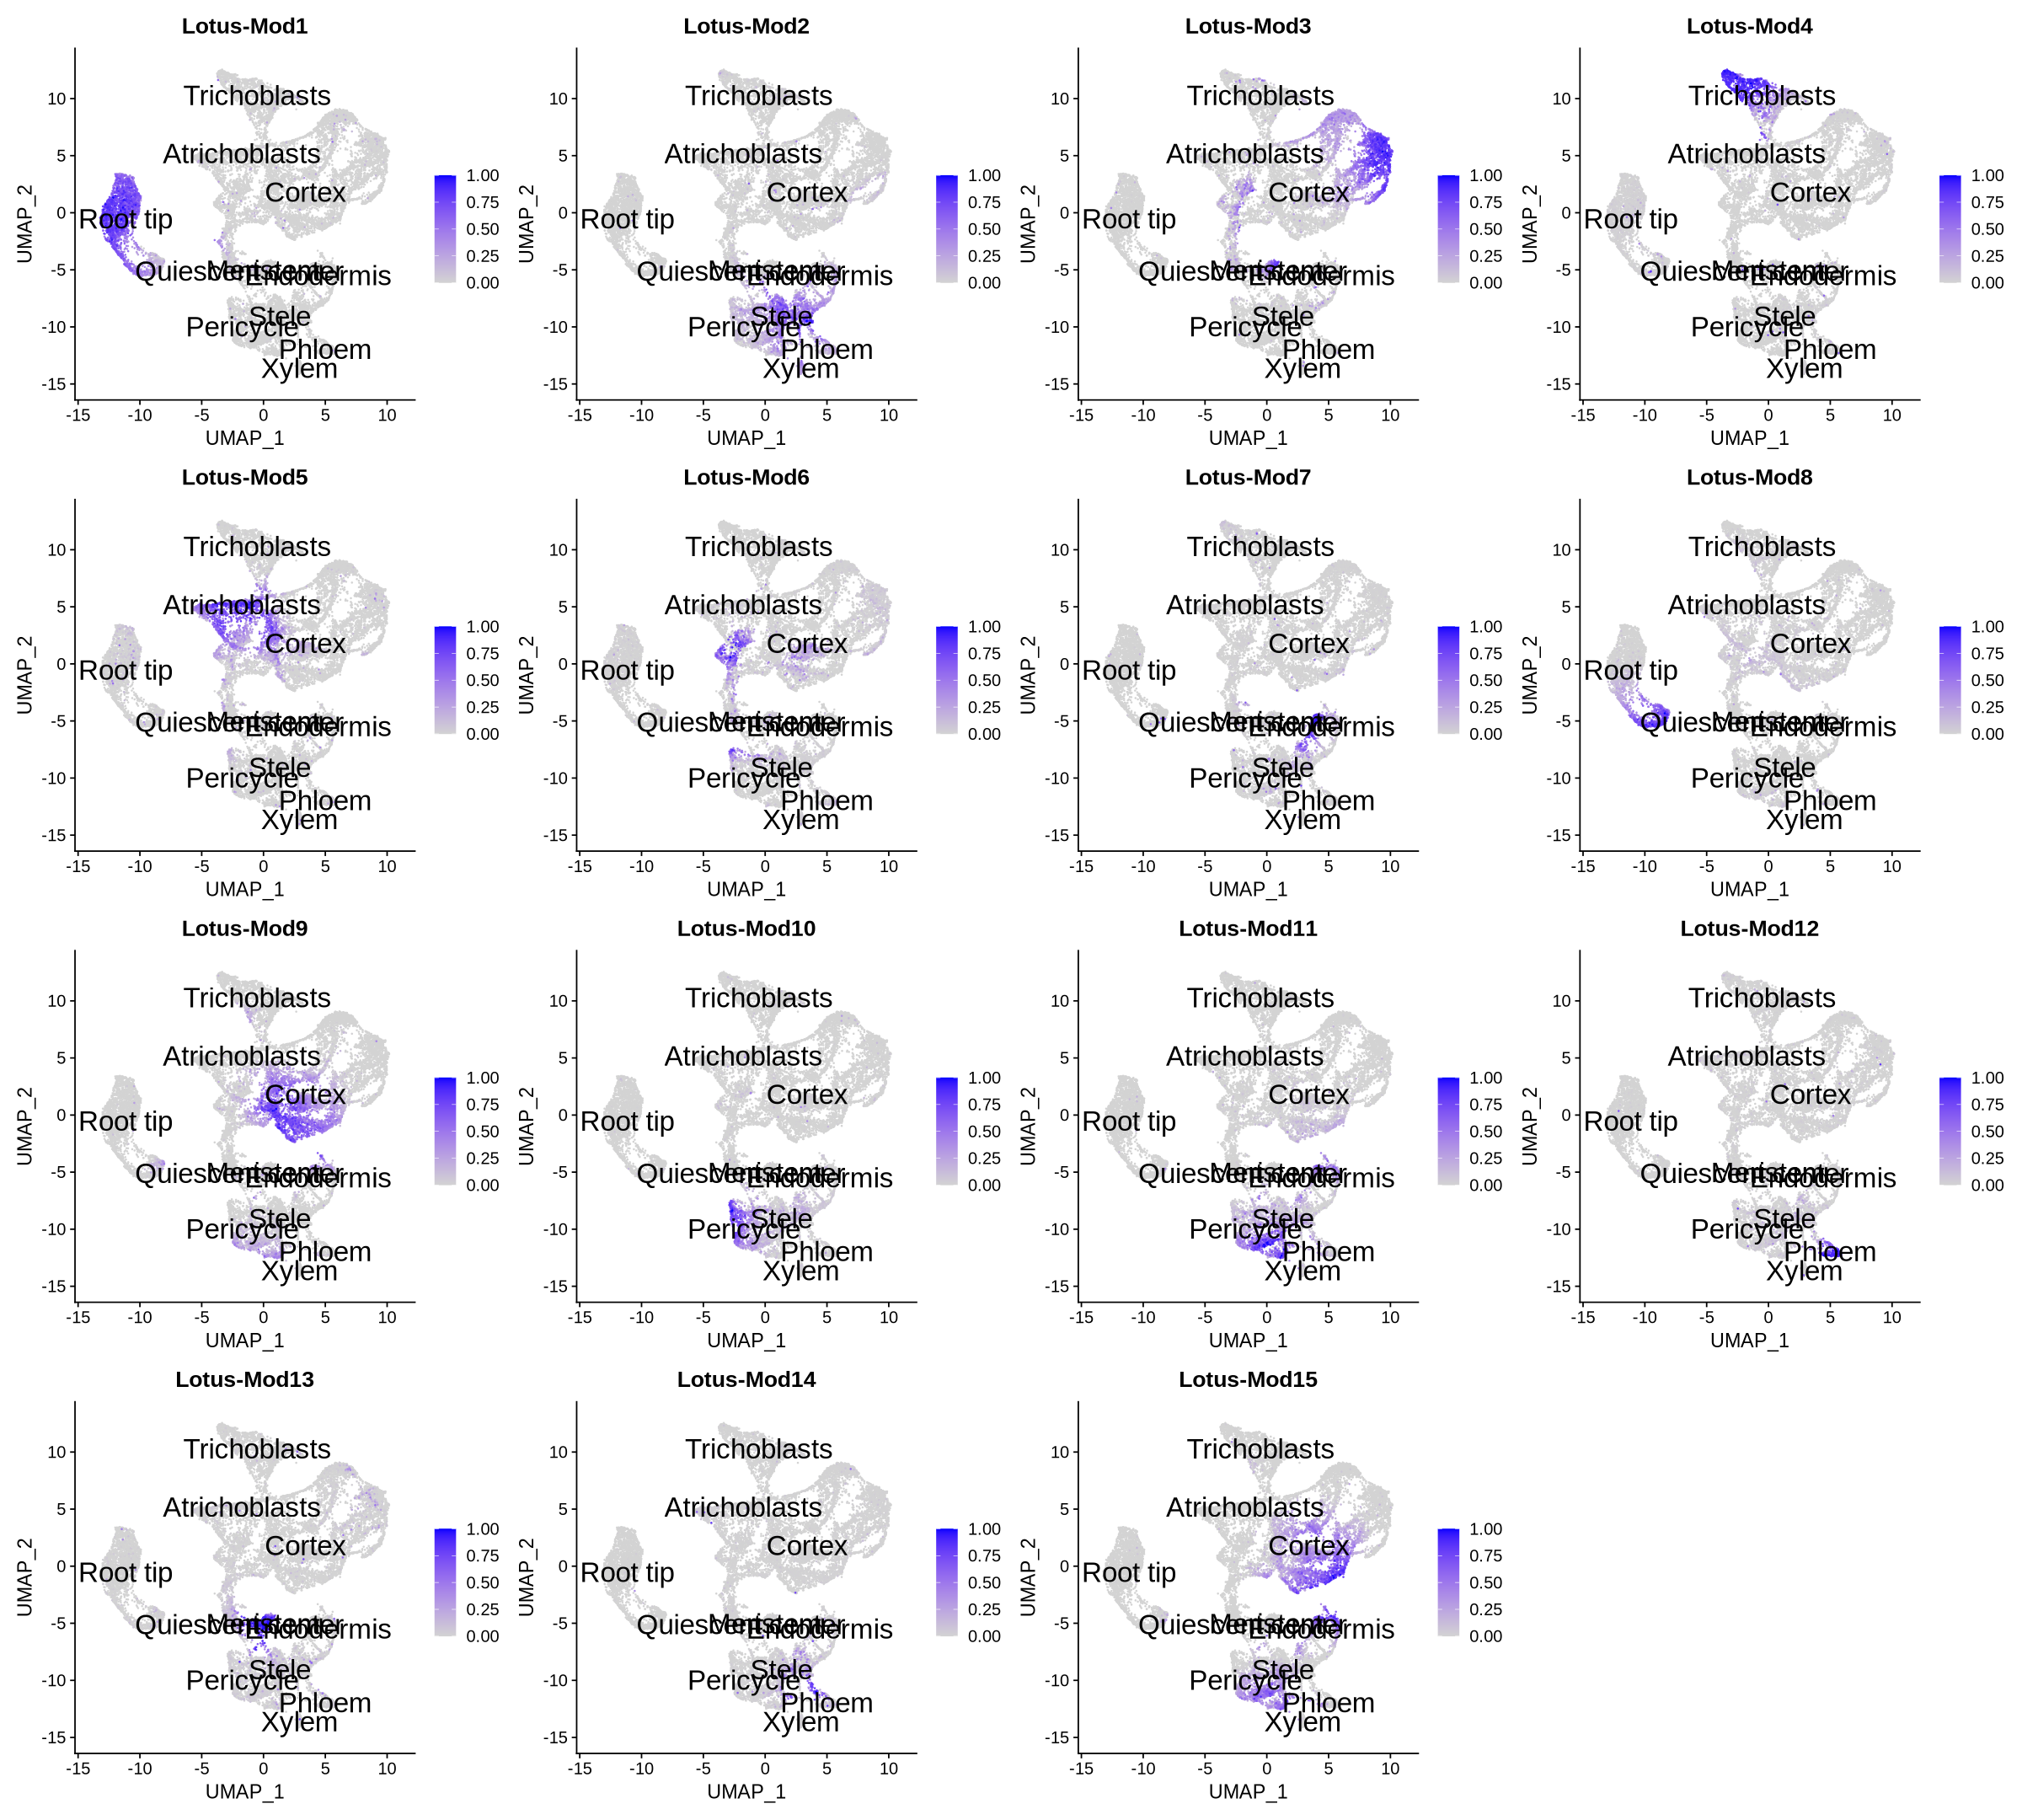
\includegraphics{tutorial-2024_files/figure-pdf/cell-135-output-3.png}

We save the seurat object and the network (because for some inscrutable
error, it cannot load together with the Seurat object when it is needed
again).

\begin{Shaded}
\begin{Highlighting}[]
\FunctionTok{SaveH5Seurat}\NormalTok{(seurat.clustered, }\StringTok{\textquotesingle{}seurat.network.h5Seurat\textquotesingle{}}\NormalTok{, }\AttributeTok{overwrite =} \ConstantTok{TRUE}\NormalTok{, }\AttributeTok{verbose=}\ConstantTok{FALSE}\NormalTok{)}
\end{Highlighting}
\end{Shaded}

\begin{verbatim}
Warning message:
“Overwriting previous file seurat.network.h5Seurat”
Creating h5Seurat file for version 3.1.5.9900
\end{verbatim}

\begin{Shaded}
\begin{Highlighting}[]
\FunctionTok{saveRDS}\NormalTok{(seurat.clustered}\SpecialCharTok{@}\NormalTok{misc, }\StringTok{"network\_lotus.RDS"}\NormalTok{)}
\end{Highlighting}
\end{Shaded}

\subsection{Differential module Expression (DME)
analysis}\label{differential-module-expression-dme-analysis}

Lastly, we can see which modules are most expressed in a specific
cluster against the others, in a similar way to differential gene
expression.

\begin{Shaded}
\begin{Highlighting}[]
\NormalTok{seurat.network }\OtherTok{\textless{}{-}} \FunctionTok{LoadH5Seurat}\NormalTok{(}\StringTok{\textquotesingle{}seurat.network.h5Seurat\textquotesingle{}}\NormalTok{, }\AttributeTok{misc=}\ConstantTok{FALSE}\NormalTok{, }\AttributeTok{verbose=}\ConstantTok{FALSE}\NormalTok{)}
\end{Highlighting}
\end{Shaded}

\begin{verbatim}
Validating h5Seurat file

Warning message:
“Adding a command log without an assay associated with it”
\end{verbatim}

\begin{verbatim}
[1] "Couldn't delete        144115188075856517"
\end{verbatim}

\begin{Shaded}
\begin{Highlighting}[]
\NormalTok{seurat.network}\SpecialCharTok{@}\NormalTok{misc }\OtherTok{\textless{}{-}} \FunctionTok{readRDS}\NormalTok{(}\StringTok{"network\_lotus.RDS"}\NormalTok{)}
\end{Highlighting}
\end{Shaded}

Here we discuss how to perform \textbf{DME testing between two different
groups}. We use the \texttt{hdWGCNA} function \texttt{FindDMEs}, which
is similar to the Seurat function FindMarkers. We use the Mann-Whitney U
test, also known as the Wilcoxon test, to compare two groups, but other
tests can be used at the user's discretion with the \texttt{test.use}
parameter.

We are interested in defining our two groups both by condition and by
choosing a cluster, for example \texttt{Cortex}. We filter DMEs by
p-value and fold-change.

\begin{Shaded}
\begin{Highlighting}[]
\NormalTok{R7Agroup }\OtherTok{\textless{}{-}}\NormalTok{ seurat.network}\SpecialCharTok{@}\NormalTok{meta.data }\SpecialCharTok{\%\textgreater{}\%} \FunctionTok{subset}\NormalTok{(Condition }\SpecialCharTok{==} \StringTok{\textquotesingle{}R7A\textquotesingle{}} \SpecialCharTok{\&}\NormalTok{ predicted.id }\SpecialCharTok{==} \StringTok{\textquotesingle{}Cortex\textquotesingle{}}\NormalTok{) }\SpecialCharTok{\%\textgreater{}\%}\NormalTok{ rownames}
\NormalTok{WTgroup }\OtherTok{\textless{}{-}}\NormalTok{ seurat.network}\SpecialCharTok{@}\NormalTok{meta.data }\SpecialCharTok{\%\textgreater{}\%} \FunctionTok{subset}\NormalTok{(Condition }\SpecialCharTok{==} \StringTok{\textquotesingle{}Control\textquotesingle{}} \SpecialCharTok{\&}\NormalTok{ predicted.id }\SpecialCharTok{==} \StringTok{\textquotesingle{}Cortex\textquotesingle{}}\NormalTok{) }\SpecialCharTok{\%\textgreater{}\%}\NormalTok{ rownames}
\end{Highlighting}
\end{Shaded}

\begin{Shaded}
\begin{Highlighting}[]
\NormalTok{DMEs }\OtherTok{\textless{}{-}} \FunctionTok{FindDMEs}\NormalTok{(}
\NormalTok{  seurat.network,}
  \AttributeTok{barcodes1 =}\NormalTok{ R7Agroup,}
  \AttributeTok{barcodes2 =}\NormalTok{ WTgroup,}
  \AttributeTok{test.use=}\StringTok{\textquotesingle{}wilcox\textquotesingle{}}\NormalTok{,}
  \AttributeTok{wgcna\_name=}\StringTok{\textquotesingle{}tutorial\textquotesingle{}}
\NormalTok{) }\SpecialCharTok{\%\textgreater{}\%} \FunctionTok{filter}\NormalTok{(p\_val\_adj }\SpecialCharTok{\textless{}} \FloatTok{0.001} \SpecialCharTok{\&} \FunctionTok{abs}\NormalTok{(avg\_log2FC)}\SpecialCharTok{\textgreater{}}\DecValTok{1}\NormalTok{) }\SpecialCharTok{\%\textgreater{}\%} \FunctionTok{select}\NormalTok{(}\SpecialCharTok{{-}}\NormalTok{p\_val)}
\end{Highlighting}
\end{Shaded}

\begin{verbatim}
[1] 17721    15
 [1] "Lotus-Mod3"  "Lotus-Mod13" "Lotus-Mod5"  "Lotus-Mod6"  "Lotus-Mod2" 
 [6] "Lotus-Mod12" "Lotus-Mod14" "Lotus-Mod7"  "Lotus-Mod10" "Lotus-Mod11"
[11] "Lotus-Mod9"  "Lotus-Mod15" "Lotus-Mod4"  "Lotus-Mod1"  "Lotus-Mod8" 
\end{verbatim}

The resulting table below is very similar to the one for differential
gene expression. Now the p-values and fold changes are referred to the
differential module expression in the inoculated cortex VS the control
cortex.

\begin{Shaded}
\begin{Highlighting}[]
\NormalTok{DMEs}
\end{Highlighting}
\end{Shaded}

A data.frame: 4 × 5

\begin{longtable}[]{@{}
  >{\raggedright\arraybackslash}p{(\columnwidth - 10\tabcolsep) * \real{0.1667}}
  >{\raggedright\arraybackslash}p{(\columnwidth - 10\tabcolsep) * \real{0.1667}}
  >{\raggedright\arraybackslash}p{(\columnwidth - 10\tabcolsep) * \real{0.1667}}
  >{\raggedright\arraybackslash}p{(\columnwidth - 10\tabcolsep) * \real{0.1667}}
  >{\raggedright\arraybackslash}p{(\columnwidth - 10\tabcolsep) * \real{0.1667}}
  >{\raggedright\arraybackslash}p{(\columnwidth - 10\tabcolsep) * \real{0.1667}}@{}}
\toprule\noalign{}
\begin{minipage}[b]{\linewidth}\raggedright
\end{minipage} & \begin{minipage}[b]{\linewidth}\raggedright
avg\_log2FC \textless dbl\textgreater{}
\end{minipage} & \begin{minipage}[b]{\linewidth}\raggedright
pct.1 \textless dbl\textgreater{}
\end{minipage} & \begin{minipage}[b]{\linewidth}\raggedright
pct.2 \textless dbl\textgreater{}
\end{minipage} & \begin{minipage}[b]{\linewidth}\raggedright
p\_val\_adj \textless dbl\textgreater{}
\end{minipage} & \begin{minipage}[b]{\linewidth}\raggedright
module \textless chr\textgreater{}
\end{minipage} \\
\midrule\noalign{}
\endhead
\bottomrule\noalign{}
\endlastfoot
Lotus-Mod11 & 1.321296 & 0.258 & 0.139 & 3.169398e-37 & Lotus-Mod11 \\
Lotus-Mod6 & 1.058396 & 0.445 & 0.329 & 2.570134e-32 & Lotus-Mod6 \\
Lotus-Mod1 & -1.213882 & 0.022 & 0.042 & 1.141514e-05 & Lotus-Mod1 \\
Lotus-Mod4 & -1.812261 & 0.063 & 0.087 & 8.976603e-04 & Lotus-Mod4 \\
\end{longtable}

We can also do a lollipop plot as in Figure~\ref{fig-lol}, where the
size of each circle is the p-value, and the x-axis is the log-fold
change. A cross on a circle means the p-value is not significant. Module
4 and 11 are very interesting because of their over- and
under-expression, though you should note the difference in percentages
is pretty small. In our case we filtered out p-values that were too
high, so we have only significant modules in the plot.

\begin{Shaded}
\begin{Highlighting}[]
\FunctionTok{options}\NormalTok{(}\AttributeTok{repr.plot.width=}\DecValTok{6}\NormalTok{, }\AttributeTok{repr.plot.height=}\DecValTok{6}\NormalTok{)}

\FunctionTok{PlotDMEsLollipop}\NormalTok{(}
\NormalTok{  seurat.network, }
\NormalTok{  DMEs, }
  \AttributeTok{wgcna\_name=}\StringTok{\textquotesingle{}tutorial\textquotesingle{}}\NormalTok{, }
  \AttributeTok{pvalue =} \StringTok{"p\_val\_adj"}\NormalTok{,}
\NormalTok{)}
\end{Highlighting}
\end{Shaded}

\begin{verbatim}
Loading required package: ggforestplot
\end{verbatim}

\begin{verbatim}
[1] "Please be aware comparison group/groups are not provided, which may casue an ERROR. PlotDMEsLollipop function will automatically assume all values are within the same group."
\end{verbatim}

\begin{figure}[H]

\centering{

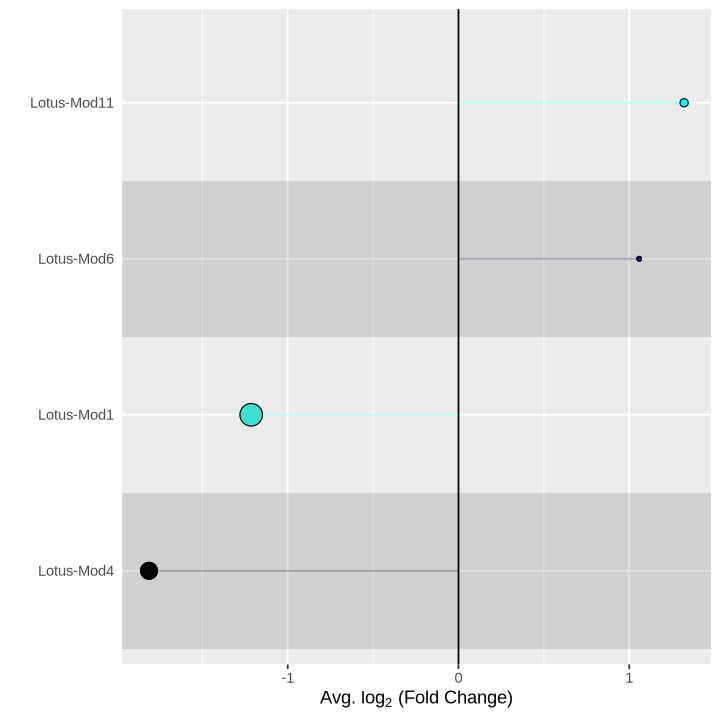
\includegraphics{tutorial-2024_files/figure-pdf/fig-lol-output-3.png}

}

\caption{\label{fig-lol}Lollipop plot that shovs the average log-fold
change of each module and the p-value (size of each circle). Crossed
circles, when present, have a non-significant p-value}

\end{figure}%

\subsubsection{One-versus-all DME
analysis}\label{one-versus-all-dme-analysis}

This is another case of DME analysis, where each cluster is tested
against the rest of the data to see which modules are differentially
expressed. We can test by cell type (\texttt{predicted.id}) or by
condition (\texttt{Condition}).

\begin{Shaded}
\begin{Highlighting}[]
\NormalTok{DMEs\_all }\OtherTok{\textless{}{-}} \FunctionTok{FindAllDMEs}\NormalTok{(}
\NormalTok{  seurat.network,}
  \AttributeTok{group.by =} \StringTok{\textquotesingle{}predicted.id\textquotesingle{}}\NormalTok{,}
  \AttributeTok{wgcna\_name =} \StringTok{\textquotesingle{}tutorial\textquotesingle{}}
\NormalTok{) }
\end{Highlighting}
\end{Shaded}

\begin{verbatim}
[1] "Cortex"
[1] "Trichoblasts"
[1] "Root tip"
[1] "Meristem"
[1] "Phloem"
[1] "Pericycle"
[1] "Stele"
[1] "Atrichoblasts"
[1] "Xylem"
[1] "Endodermis"
[1] "Quiescent center"
\end{verbatim}

The table is usually big, but you can choose to filter by various
parameters as below, and to look only at one cluster of interest

\begin{Shaded}
\begin{Highlighting}[]
\NormalTok{DMEs\_cortex }\OtherTok{\textless{}{-}}\NormalTok{ DMEs\_all }\SpecialCharTok{\%\textgreater{}\%} \FunctionTok{filter}\NormalTok{(p\_val\_adj }\SpecialCharTok{\textless{}}\NormalTok{ .}\DecValTok{001} \SpecialCharTok{\&} \FunctionTok{abs}\NormalTok{(avg\_log2FC)}\SpecialCharTok{\textgreater{}}\DecValTok{1} 
                                       \SpecialCharTok{\&} \FunctionTok{is.finite}\NormalTok{(avg\_log2FC)}
                                       \SpecialCharTok{\&}\NormalTok{ group}\SpecialCharTok{==}\StringTok{\textquotesingle{}Cortex\textquotesingle{}}\NormalTok{)}
\end{Highlighting}
\end{Shaded}

The DME analysis results in a lot of significant results for the cortex.
But we can see that \texttt{pct.1} and \texttt{pct.2} vary a lot. Module
12 has more than 50\% of the cells expressing the module, and 7\% in the
rest of the data, while Module 20 has percentages of 52\% vs 22\%. Here
it is always best to report those percentages and log-fold changes
starting from the highest ones.

\begin{Shaded}
\begin{Highlighting}[]
\NormalTok{DMEs\_cortex}
\end{Highlighting}
\end{Shaded}

A data.frame: 14 × 7

\begin{longtable}[]{@{}
  >{\raggedright\arraybackslash}p{(\columnwidth - 14\tabcolsep) * \real{0.1250}}
  >{\raggedright\arraybackslash}p{(\columnwidth - 14\tabcolsep) * \real{0.1250}}
  >{\raggedright\arraybackslash}p{(\columnwidth - 14\tabcolsep) * \real{0.1250}}
  >{\raggedright\arraybackslash}p{(\columnwidth - 14\tabcolsep) * \real{0.1250}}
  >{\raggedright\arraybackslash}p{(\columnwidth - 14\tabcolsep) * \real{0.1250}}
  >{\raggedright\arraybackslash}p{(\columnwidth - 14\tabcolsep) * \real{0.1250}}
  >{\raggedright\arraybackslash}p{(\columnwidth - 14\tabcolsep) * \real{0.1250}}
  >{\raggedright\arraybackslash}p{(\columnwidth - 14\tabcolsep) * \real{0.1250}}@{}}
\toprule\noalign{}
\begin{minipage}[b]{\linewidth}\raggedright
\end{minipage} & \begin{minipage}[b]{\linewidth}\raggedright
p\_val \textless dbl\textgreater{}
\end{minipage} & \begin{minipage}[b]{\linewidth}\raggedright
avg\_log2FC \textless dbl\textgreater{}
\end{minipage} & \begin{minipage}[b]{\linewidth}\raggedright
pct.1 \textless dbl\textgreater{}
\end{minipage} & \begin{minipage}[b]{\linewidth}\raggedright
pct.2 \textless dbl\textgreater{}
\end{minipage} & \begin{minipage}[b]{\linewidth}\raggedright
p\_val\_adj \textless dbl\textgreater{}
\end{minipage} & \begin{minipage}[b]{\linewidth}\raggedright
module \textless chr\textgreater{}
\end{minipage} & \begin{minipage}[b]{\linewidth}\raggedright
group \textless chr\textgreater{}
\end{minipage} \\
\midrule\noalign{}
\endhead
\bottomrule\noalign{}
\endlastfoot
Cortex.Lotus-Mod3 & 0.000000e+00 & 2.690457 & 0.518 & 0.149 &
0.000000e+00 & Lotus-Mod3 & Cortex \\
Cortex.Lotus-Mod6 & 0.000000e+00 & 2.516551 & 0.397 & 0.137 &
0.000000e+00 & Lotus-Mod6 & Cortex \\
Cortex.Lotus-Mod2 & 0.000000e+00 & -4.225120 & 0.075 & 0.348 &
0.000000e+00 & Lotus-Mod2 & Cortex \\
Cortex.Lotus-Mod12 & 0.000000e+00 & -4.736902 & 0.038 & 0.283 &
0.000000e+00 & Lotus-Mod12 & Cortex \\
Cortex.Lotus-Mod9 & 0.000000e+00 & 2.309667 & 0.522 & 0.249 &
0.000000e+00 & Lotus-Mod9 & Cortex \\
Cortex.Lotus-Mod1 & 0.000000e+00 & -5.372586 & 0.031 & 0.284 &
0.000000e+00 & Lotus-Mod1 & Cortex \\
Cortex.Lotus-Mod14 & 1.424592e-288 & -3.210875 & 0.077 & 0.295 &
2.136888e-287 & Lotus-Mod14 & Cortex \\
Cortex.Lotus-Mod10 & 3.164844e-256 & -4.539404 & 0.075 & 0.266 &
4.747266e-255 & Lotus-Mod10 & Cortex \\
Cortex.Lotus-Mod15 & 2.013474e-254 & 1.032737 & 0.476 & 0.218 &
3.020212e-253 & Lotus-Mod15 & Cortex \\
Cortex.Lotus-Mod4 & 8.327387e-179 & -3.730921 & 0.073 & 0.224 &
1.249108e-177 & Lotus-Mod4 & Cortex \\
Cortex.Lotus-Mod11 & 1.287590e-108 & -2.435203 & 0.209 & 0.325 &
1.931384e-107 & Lotus-Mod11 & Cortex \\
Cortex.Lotus-Mod7 & 1.020206e-39 & -2.764012 & 0.122 & 0.188 &
1.530309e-38 & Lotus-Mod7 & Cortex \\
Cortex.Lotus-Mod8 & 2.830229e-24 & -2.096240 & 0.246 & 0.291 &
4.245343e-23 & Lotus-Mod8 & Cortex \\
Cortex.Lotus-Mod13 & 3.424949e-07 & -1.448706 & 0.172 & 0.202 &
5.137423e-06 & Lotus-Mod13 & Cortex \\
\end{longtable}

You can look at any other cluster. For example trichoblasts. Here you
can see how module 4 pops up as being basically entirely expressed only
in Trichoblasts.

\begin{Shaded}
\begin{Highlighting}[]
\NormalTok{DMEs\_tricho }\OtherTok{\textless{}{-}}\NormalTok{ DMEs\_all }\SpecialCharTok{\%\textgreater{}\%} \FunctionTok{filter}\NormalTok{(p\_val\_adj }\SpecialCharTok{\textless{}}\NormalTok{ .}\DecValTok{001} \SpecialCharTok{\&} \FunctionTok{abs}\NormalTok{(avg\_log2FC)}\SpecialCharTok{\textgreater{}}\DecValTok{1} 
                                       \SpecialCharTok{\&} \FunctionTok{is.finite}\NormalTok{(avg\_log2FC)}
                                       \SpecialCharTok{\&}\NormalTok{ group}\SpecialCharTok{==}\StringTok{\textquotesingle{}Trichoblasts\textquotesingle{}}\NormalTok{)}
\end{Highlighting}
\end{Shaded}

\begin{Shaded}
\begin{Highlighting}[]
\NormalTok{DMEs\_tricho}
\end{Highlighting}
\end{Shaded}

A data.frame: 15 × 7

\begin{longtable}[]{@{}
  >{\raggedright\arraybackslash}p{(\columnwidth - 14\tabcolsep) * \real{0.1250}}
  >{\raggedright\arraybackslash}p{(\columnwidth - 14\tabcolsep) * \real{0.1250}}
  >{\raggedright\arraybackslash}p{(\columnwidth - 14\tabcolsep) * \real{0.1250}}
  >{\raggedright\arraybackslash}p{(\columnwidth - 14\tabcolsep) * \real{0.1250}}
  >{\raggedright\arraybackslash}p{(\columnwidth - 14\tabcolsep) * \real{0.1250}}
  >{\raggedright\arraybackslash}p{(\columnwidth - 14\tabcolsep) * \real{0.1250}}
  >{\raggedright\arraybackslash}p{(\columnwidth - 14\tabcolsep) * \real{0.1250}}
  >{\raggedright\arraybackslash}p{(\columnwidth - 14\tabcolsep) * \real{0.1250}}@{}}
\toprule\noalign{}
\begin{minipage}[b]{\linewidth}\raggedright
\end{minipage} & \begin{minipage}[b]{\linewidth}\raggedright
p\_val \textless dbl\textgreater{}
\end{minipage} & \begin{minipage}[b]{\linewidth}\raggedright
avg\_log2FC \textless dbl\textgreater{}
\end{minipage} & \begin{minipage}[b]{\linewidth}\raggedright
pct.1 \textless dbl\textgreater{}
\end{minipage} & \begin{minipage}[b]{\linewidth}\raggedright
pct.2 \textless dbl\textgreater{}
\end{minipage} & \begin{minipage}[b]{\linewidth}\raggedright
p\_val\_adj \textless dbl\textgreater{}
\end{minipage} & \begin{minipage}[b]{\linewidth}\raggedright
module \textless chr\textgreater{}
\end{minipage} & \begin{minipage}[b]{\linewidth}\raggedright
group \textless chr\textgreater{}
\end{minipage} \\
\midrule\noalign{}
\endhead
\bottomrule\noalign{}
\endlastfoot
Trichoblasts.Lotus-Mod4 & 0.000000e+00 & 6.462799 & 0.998 & 0.078 &
0.000000e+00 & Lotus-Mod4 & Trichoblasts \\
Trichoblasts.Lotus-Mod15 & 4.589076e-165 & -6.220812 & 0.016 & 0.357 &
6.883613e-164 & Lotus-Mod15 & Trichoblasts \\
Trichoblasts.Lotus-Mod11 & 2.472972e-134 & -6.784385 & 0.011 & 0.303 &
3.709458e-133 & Lotus-Mod11 & Trichoblasts \\
Trichoblasts.Lotus-Mod9 & 1.165473e-129 & -3.592430 & 0.095 & 0.390 &
1.748210e-128 & Lotus-Mod9 & Trichoblasts \\
Trichoblasts.Lotus-Mod3 & 6.823088e-111 & -4.113294 & 0.065 & 0.327 &
1.023463e-109 & Lotus-Mod3 & Trichoblasts \\
Trichoblasts.Lotus-Mod6 & 7.331605e-111 & -5.105053 & 0.014 & 0.268 &
1.099741e-109 & Lotus-Mod6 & Trichoblasts \\
Trichoblasts.Lotus-Mod2 & 1.103509e-101 & -4.652608 & 0.016 & 0.255 &
1.655264e-100 & Lotus-Mod2 & Trichoblasts \\
Trichoblasts.Lotus-Mod10 & 1.334983e-80 & -6.542761 & 0.009 & 0.204 &
2.002475e-79 & Lotus-Mod10 & Trichoblasts \\
Trichoblasts.Lotus-Mod12 & 5.703476e-72 & -5.346382 & 0.017 & 0.197 &
8.555215e-71 & Lotus-Mod12 & Trichoblasts \\
Trichoblasts.Lotus-Mod14 & 9.752613e-68 & -3.932097 & 0.037 & 0.221 &
1.462892e-66 & Lotus-Mod14 & Trichoblasts \\
Trichoblasts.Lotus-Mod5 & 1.462617e-64 & -3.455537 & 0.089 & 0.271 &
2.193925e-63 & Lotus-Mod5 & Trichoblasts \\
Trichoblasts.Lotus-Mod13 & 1.126768e-63 & -2.689731 & 0.032 & 0.205 &
1.690151e-62 & Lotus-Mod13 & Trichoblasts \\
Trichoblasts.Lotus-Mod1 & 6.001523e-29 & -5.077260 & 0.090 & 0.187 &
9.002285e-28 & Lotus-Mod1 & Trichoblasts \\
Trichoblasts.Lotus-Mod8 & 9.594551e-24 & -2.423585 & 0.179 & 0.282 &
1.439183e-22 & Lotus-Mod8 & Trichoblasts \\
Trichoblasts.Lotus-Mod7 & 6.536989e-21 & -3.664154 & 0.083 & 0.168 &
9.805484e-20 & Lotus-Mod7 & Trichoblasts \\
\end{longtable}

For better visualization, you can always use the lolliplot plots using
the correct table as an argument, so that you can plot multiple
instances for the various clusters. In Figure~\ref{fig-lol2} we plot
boyh for cortex and trichoblasts from the tables determined in the code
above.

\begin{Shaded}
\begin{Highlighting}[]
\FunctionTok{options}\NormalTok{(}\AttributeTok{repr.plot.width=}\DecValTok{12}\NormalTok{, }\AttributeTok{repr.plot.height=}\DecValTok{6}\NormalTok{)}

\CommentTok{\#lollipop with cortex table}
\NormalTok{p1 }\OtherTok{\textless{}{-}} \FunctionTok{PlotDMEsLollipop}\NormalTok{(}
\NormalTok{  seurat.network, }
\NormalTok{  DMEs\_cortex, }
  \AttributeTok{wgcna\_name=}\StringTok{\textquotesingle{}tutorial\textquotesingle{}}\NormalTok{, }
  \AttributeTok{pvalue =} \StringTok{"p\_val\_adj"}\NormalTok{,}
\NormalTok{)}

\CommentTok{\#lollipop with trichoblasts table}
\NormalTok{p2 }\OtherTok{\textless{}{-}} \FunctionTok{PlotDMEsLollipop}\NormalTok{(}
\NormalTok{  seurat.network, }
\NormalTok{  DMEs\_tricho, }
  \AttributeTok{wgcna\_name=}\StringTok{\textquotesingle{}tutorial\textquotesingle{}}\NormalTok{, }
  \AttributeTok{pvalue =} \StringTok{"p\_val\_adj"}\NormalTok{,}
\NormalTok{)}

\CommentTok{\#plot an add a title}
\NormalTok{p1 }\SpecialCharTok{+} \FunctionTok{ggtitle}\NormalTok{(}\StringTok{"DMEs of Cortex VS data"}\NormalTok{) }\SpecialCharTok{+} 
\NormalTok{p2 }\SpecialCharTok{+} \FunctionTok{ggtitle}\NormalTok{(}\StringTok{"DMEs of Trichoblasts VS data"}\NormalTok{)}
\end{Highlighting}
\end{Shaded}

\begin{verbatim}
[1] "Please be aware comparison group/groups are not provided, which may casue an ERROR. PlotDMEsLollipop function will automatically assume all values are within the same group."
[1] "Please be aware comparison group/groups are not provided, which may casue an ERROR. PlotDMEsLollipop function will automatically assume all values are within the same group."
\end{verbatim}

\begin{figure}[H]

\centering{

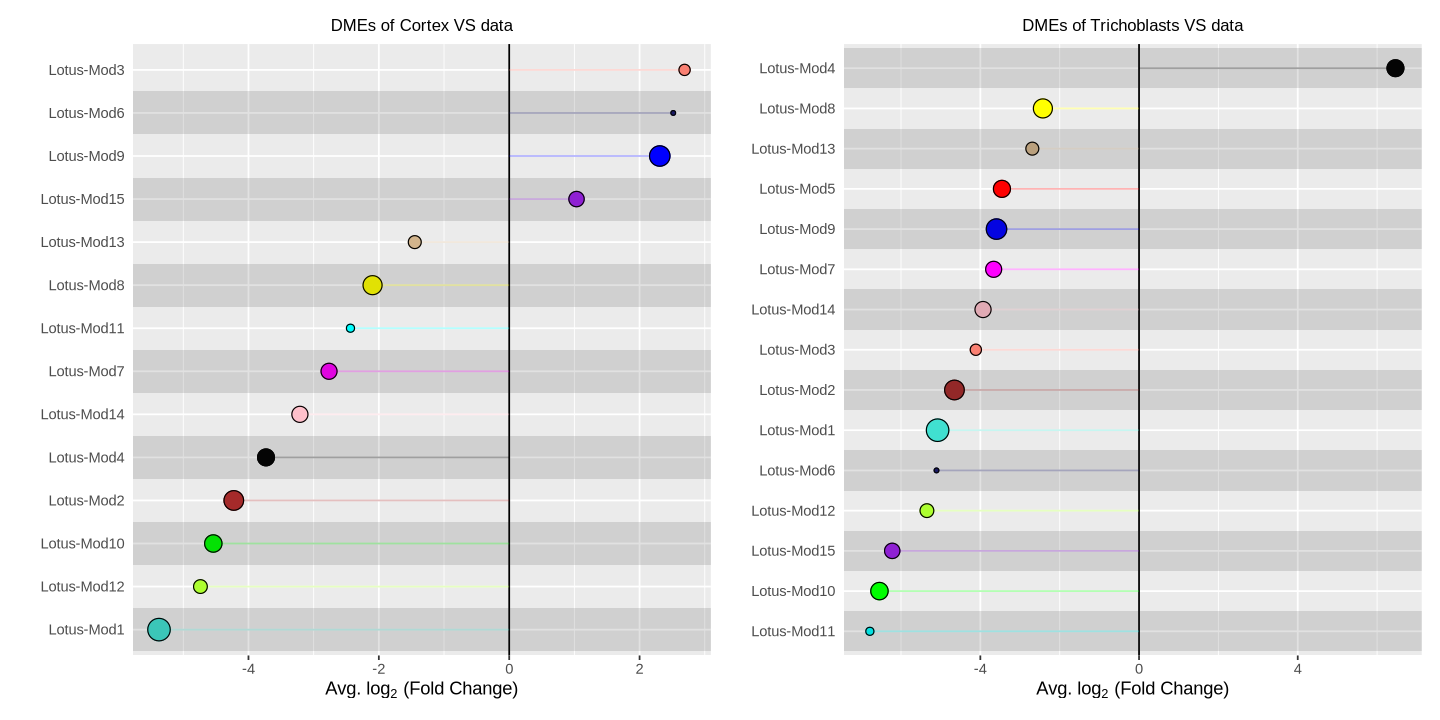
\includegraphics{tutorial-2024_files/figure-pdf/fig-lol2-output-2.png}

}

\caption{\label{fig-lol2}Lollipop plot that shovs the average log-fold
change of each module and the p-value (size of each circle). Crossed
circles, when present, have a non-significant p-value. Plotting
lolliplot plots for various clusters can be useful to detect modules
being simultaneously significant.}

\end{figure}%

\begin{tcolorbox}[enhanced jigsaw, toprule=.15mm, coltitle=black, colframe=quarto-callout-note-color-frame, colback=white, colbacktitle=quarto-callout-note-color!10!white, opacityback=0, arc=.35mm, breakable, rightrule=.15mm, titlerule=0mm, leftrule=.75mm, bottomtitle=1mm, toptitle=1mm, title=\textcolor{quarto-callout-note-color}{\faInfo}\hspace{0.5em}{Wrapping Up}, bottomrule=.15mm, left=2mm, opacitybacktitle=0.6]

This is the end of the tutorial. We have not shown much biological
conclusion from the analysis - this is something that comes out by
studying for example the GO terms of the various genes and modules
identified. The scope of the tutorial was mainly to give all the means
to perform your own analysis, from which you can then gain biological
insight.

If you are interested in more resources to learn single cell analysis,
you can find them at some of our courses. We have other single-cell
analysis tutorials including different tools at

\begin{itemize}
\tightlist
\item
  \textbf{Introduction to NGS data analysis} (found in the
  \texttt{Genomics\ Sandbox}
  \textbf{\href{https://cloud.sdu.dk/app/jobs/create?app=genomics&version=2023.03.01}{at
  this link}} - note that this is in the \texttt{python} language )
\item
  \textbf{Introduction to scRNAseq analysis in R} (found in the
  \texttt{Transcriptomics\ Sandbox}
  \textbf{\href{https://cloud.sdu.dk/app/jobs/create?app=transcriptomics&version=2023.11}{at
  this link}} )
\end{itemize}

You can also find a lot of material in the
\textbf{\href{https://satijalab.org/seurat/articles/get_started.html}{\texttt{Seurat}
webpage}}. If you create a new notebook in this environment, you are
likely to have all the packages needed to try the \texttt{Seurat}
tutorials.

\end{tcolorbox}

\phantomsection\label{refs}
\begin{CSLReferences}{1}{0}
\bibitem[\citeproctext]{ref-adossa_computational_2021}
Adossa, Nigatu, Sofia Khan, Kalle T. Rytkönen, and Laura L. Elo. 2021.
{``Computational Strategies for Single-Cell Multi-Omics Integration.''}
\emph{Computational and Structural Biotechnology Journal} 19: 2588--96.
\url{https://doi.org/10.1016/j.csbj.2021.04.060}.

\bibitem[\citeproctext]{ref-becht_dimensionality_2019}
Becht, Etienne, Leland McInnes, John Healy, Charles-Antoine Dutertre,
Immanuel W H Kwok, Lai Guan Ng, Florent Ginhoux, and Evan W Newell.
2019. {``Dimensionality Reduction for Visualizing Single-Cell Data Using
{UMAP}.''} \emph{Nature Biotechnology} 37 (1): 38--44.
\url{https://doi.org/10.1038/nbt.4314}.

\bibitem[\citeproctext]{ref-cheng_review_2023}
Cheng, Changde, Wenan Chen, Hongjian Jin, and Xiang Chen. 2023. {``A
{Review} of {Single}-{Cell} {RNA}-{Seq} {Annotation}, {Integration}, and
{Cell}--{Cell} {Communication}.''} \emph{Cells} 12 (15): 1970.
\url{https://doi.org/10.3390/cells12151970}.

\bibitem[\citeproctext]{ref-fleming_unsupervised_2023}
Fleming, Stephen J., Mark D. Chaffin, Alessandro Arduini, Amer-Denis
Akkad, Eric Banks, John C. Marioni, Anthony A. Philippakis, Patrick T.
Ellinor, and Mehrtash Babadi. 2023. {``Unsupervised Removal of
Systematic Background Noise from Droplet-Based Single-Cell Experiments
Using {CellBender}.''} \emph{Nature Methods} 20 (9): 1323--35.
\url{https://doi.org/10.1038/s41592-023-01943-7}.

\bibitem[\citeproctext]{ref-frank_single-cell_2023}
Frank, Manuel, Lavinia Ioana Fechete, Francesca Tedeschi, Marcin
Nadzieja, Malita Malou Malekzadeh Nørgaard, Jesus Montiel, Kasper
Røjkjær Andersen, Mikkel H. Schierup, Dugald Reid, and Stig Uggerhøj
Andersen. 2023. {``Single-Cell Analysis Identifies Genes Facilitating
Rhizobium Infection in {Lotus} Japonicus.''} \emph{Nature
Communications} 14 (November): 7171.
\url{https://doi.org/10.1038/s41467-023-42911-1}.

\bibitem[\citeproctext]{ref-hafemeister_normalization_2019}
Hafemeister, Christoph, and Rahul Satija. 2019. {``Normalization and
Variance Stabilization of Single-Cell {RNA}-Seq Data Using Regularized
Negative Binomial Regression.''} \emph{Genome Biology} 20 (1): 296.
\url{https://doi.org/10.1186/s13059-019-1874-1}.

\bibitem[\citeproctext]{ref-heumos_best_2023}
Heumos, Lukas, Anna C. Schaar, Christopher Lance, Anastasia
Litinetskaya, Felix Drost, Luke Zappia, Malte D. Lücken, et al. 2023.
{``Best Practices for Single-Cell Analysis Across Modalities.''}
\emph{Nature Reviews Genetics} 24 (8): 550--72.
\url{https://doi.org/10.1038/s41576-023-00586-w}.

\bibitem[\citeproctext]{ref-korsunsky_fast_2019}
Korsunsky, Ilya, Nghia Millard, Jean Fan, Kamil Slowikowski, Fan Zhang,
Kevin Wei, Yuriy Baglaenko, Michael Brenner, Po-ru Loh, and Soumya
Raychaudhuri. 2019. {``Fast, Sensitive and Accurate Integration of
Single-Cell Data with {Harmony}.''} \emph{Nature Methods} 16 (12):
1289--96. \url{https://doi.org/10.1038/s41592-019-0619-0}.

\bibitem[\citeproctext]{ref-langfelder_eigengene_2007}
Langfelder, Peter, and Steve Horvath. 2007. {``Eigengene Networks for
Studying the Relationships Between Co-Expression Modules.''} \emph{BMC
Systems Biology} 1 (1): 54.
\url{https://doi.org/10.1186/1752-0509-1-54}.

\bibitem[\citeproctext]{ref-luecken_current_2019}
Luecken, Malte D, and Fabian J Theis. 2019. {``Current Best Practices in
Single‐cell {RNA}‐seq Analysis: A Tutorial.''} \emph{Molecular Systems
Biology} 15 (6): e8746. \url{https://doi.org/10.15252/msb.20188746}.

\bibitem[\citeproctext]{ref-mcginnis_doubletfinder_2019}
McGinnis, Christopher S., Lyndsay M. Murrow, and Zev J. Gartner. 2019.
{``{DoubletFinder}: {Doublet} {Detection} in {Single}-{Cell} {RNA}
{Sequencing} {Data} {Using} {Artificial} {Nearest} {Neighbors}.''}
\emph{Cell Systems} 8 (4): 329--337.e4.
\url{https://doi.org/10.1016/j.cels.2019.03.003}.

\bibitem[\citeproctext]{ref-mcinnes_umap_2018}
McInnes, Leland, John Healy, Nathaniel Saul, and Lukas Großberger. 2018.
{``{UMAP}: {Uniform} {Manifold} {Approximation} and {Projection}.''}
\emph{Journal of Open Source Software} 3 (29): 861.
\url{https://doi.org/10.21105/joss.00861}.

\bibitem[\citeproctext]{ref-morabito_hdwgcna_2023}
Morabito, Samuel, Fairlie Reese, Negin Rahimzadeh, Emily Miyoshi, and
Vivek Swarup. 2023. {``{hdWGCNA} Identifies Co-Expression Networks in
High-Dimensional Transcriptomics Data.''} \emph{Cell Reports Methods} 3
(6): 100498. \url{https://doi.org/10.1016/j.crmeth.2023.100498}.

\bibitem[\citeproctext]{ref-stuart_comprehensive_2019}
Stuart, Tim, Andrew Butler, Paul Hoffman, Christoph Hafemeister,
Efthymia Papalexi, William M. Mauck, Yuhan Hao, Marlon Stoeckius, Peter
Smibert, and Rahul Satija. 2019. {``Comprehensive {Integration} of
{Single}-{Cell} {Data}.''} \emph{Cell} 177 (7): 1888--1902.e21.
\url{https://doi.org/10.1016/j.cell.2019.05.031}.

\bibitem[\citeproctext]{ref-traag_louvain_2019}
Traag, V. A., L. Waltman, and N. J. Van Eck. 2019. {``From {Louvain} to
{Leiden}: Guaranteeing Well-Connected Communities.''} \emph{Scientific
Reports} 9 (1): 5233. \url{https://doi.org/10.1038/s41598-019-41695-z}.

\bibitem[\citeproctext]{ref-xiang_comparison_2021}
Xiang, Ruizhi, Wencan Wang, Lei Yang, Shiyuan Wang, Chaohan Xu, and
Xiaowen Chen. 2021. {``A {Comparison} for {Dimensionality} {Reduction}
{Methods} of {Single}-{Cell} {RNA}-Seq {Data}.''} \emph{Frontiers in
Genetics} 12 (March): 646936.
\url{https://doi.org/10.3389/fgene.2021.646936}.

\bibitem[\citeproctext]{ref-xinming_seurat_2022}
Xinming, Tu. 2022. {``Seurat {CCA}? {It}'s Just a Simple Extension of
{PCA}!''} \url{https://xinmingtu.cn/blog/2022/CCA_dual_PCA/}.

\bibitem[\citeproctext]{ref-young_soupx_2020}
Young, Matthew D, and Sam Behjati. 2020. {``{SoupX} Removes Ambient
{RNA} Contamination from Droplet-Based Single-Cell {RNA} Sequencing
Data.''} \emph{GigaScience} 9 (12): giaa151.
\url{https://doi.org/10.1093/gigascience/giaa151}.

\end{CSLReferences}



\end{document}
